\documentclass[twoside]{book}

% Packages required by doxygen
\usepackage{fixltx2e}
\usepackage{calc}
\usepackage{doxygen}
\usepackage[export]{adjustbox} % also loads graphicx
\usepackage{graphicx}
\usepackage[utf8]{inputenc}
\usepackage{makeidx}
\usepackage{multicol}
\usepackage{multirow}
\PassOptionsToPackage{warn}{textcomp}
\usepackage{textcomp}
\usepackage[nointegrals]{wasysym}
\usepackage[table]{xcolor}

% Font selection
\usepackage[T1]{fontenc}
\usepackage[scaled=.90]{helvet}
\usepackage{courier}
\usepackage{amssymb}
\usepackage{sectsty}
\renewcommand{\familydefault}{\sfdefault}
\allsectionsfont{%
  \fontseries{bc}\selectfont%
  \color{darkgray}%
}
\renewcommand{\DoxyLabelFont}{%
  \fontseries{bc}\selectfont%
  \color{darkgray}%
}
\newcommand{\+}{\discretionary{\mbox{\scriptsize$\hookleftarrow$}}{}{}}

% Page & text layout
\usepackage{geometry}
\geometry{%
  a4paper,%
  top=2.5cm,%
  bottom=2.5cm,%
  left=2.5cm,%
  right=2.5cm%
}
\tolerance=750
\hfuzz=15pt
\hbadness=750
\setlength{\emergencystretch}{15pt}
\setlength{\parindent}{0cm}
\setlength{\parskip}{3ex plus 2ex minus 2ex}
\makeatletter
\renewcommand{\paragraph}{%
  \@startsection{paragraph}{4}{0ex}{-1.0ex}{1.0ex}{%
    \normalfont\normalsize\bfseries\SS@parafont%
  }%
}
\renewcommand{\subparagraph}{%
  \@startsection{subparagraph}{5}{0ex}{-1.0ex}{1.0ex}{%
    \normalfont\normalsize\bfseries\SS@subparafont%
  }%
}
\makeatother

% Headers & footers
\usepackage{fancyhdr}
\pagestyle{fancyplain}
\fancyhead[LE]{\fancyplain{}{\bfseries\thepage}}
\fancyhead[CE]{\fancyplain{}{}}
\fancyhead[RE]{\fancyplain{}{\bfseries\leftmark}}
\fancyhead[LO]{\fancyplain{}{\bfseries\rightmark}}
\fancyhead[CO]{\fancyplain{}{}}
\fancyhead[RO]{\fancyplain{}{\bfseries\thepage}}
\fancyfoot[LE]{\fancyplain{}{}}
\fancyfoot[CE]{\fancyplain{}{}}
\fancyfoot[RE]{\fancyplain{}{\bfseries\scriptsize Generated by Doxygen }}
\fancyfoot[LO]{\fancyplain{}{\bfseries\scriptsize Generated by Doxygen }}
\fancyfoot[CO]{\fancyplain{}{}}
\fancyfoot[RO]{\fancyplain{}{}}
\renewcommand{\footrulewidth}{0.4pt}
\renewcommand{\chaptermark}[1]{%
  \markboth{#1}{}%
}
\renewcommand{\sectionmark}[1]{%
  \markright{\thesection\ #1}%
}

% Indices & bibliography
\usepackage{natbib}
\usepackage[titles]{tocloft}
\setcounter{tocdepth}{3}
\setcounter{secnumdepth}{5}
\makeindex

% Hyperlinks (required, but should be loaded last)
\usepackage{ifpdf}
\ifpdf
  \usepackage[pdftex,pagebackref=true]{hyperref}
\else
  \usepackage[ps2pdf,pagebackref=true]{hyperref}
\fi
\hypersetup{%
  colorlinks=true,%
  linkcolor=blue,%
  citecolor=blue,%
  unicode%
}

% Custom commands
\newcommand{\clearemptydoublepage}{%
  \newpage{\pagestyle{empty}\cleardoublepage}%
}

\usepackage{caption}
\captionsetup{labelsep=space,justification=centering,font={bf},singlelinecheck=off,skip=4pt,position=top}

%===== C O N T E N T S =====

\begin{document}

% Titlepage & ToC
\hypersetup{pageanchor=false,
             bookmarksnumbered=true,
             pdfencoding=unicode
            }
\pagenumbering{alph}
\begin{titlepage}
\vspace*{7cm}
\begin{center}%
{\Large Depth Clustering }\\
\vspace*{1cm}
{\large Generated by Doxygen 1.8.13}\\
\end{center}
\end{titlepage}
\clearemptydoublepage
\pagenumbering{roman}
\tableofcontents
\clearemptydoublepage
\pagenumbering{arabic}
\hypersetup{pageanchor=true}

%--- Begin generated contents ---
\chapter{Depth Clustering}
\label{index}\hypertarget{index}{}Ubuntu 14.\+04

\href{https://travis-ci.org/PRBonn/depth_clustering}{\tt } \href{https://www.codacy.com/project/zabugr/depth_clustering/dashboard?utm_source=github.com&amp;utm_medium=referral&amp;utm_content=PRBonn/depth_clustering&amp;utm_campaign=Badge_Grade_Dashboard}{\tt } \href{https://coveralls.io/github/PRBonn/depth_clustering}{\tt }

This is a fast and robust algorithm to segment point clouds taken with Velodyne sensor into objects. It works with all available Velodyne sensors, i.\+e. 16, 32 and 64 beam ones.

Check out a video that shows all objects outlined in orange\+: \href{https://www.youtube.com/watch?v=UXHX9kFGXfg}{\tt html doc/pics/depth\+\_\+clustering\+\_\+new\+\_\+short\+\_\+1.\+gif \char`\"{}\+Segmentation illustration\char`\"{}}

\subsection*{Prerequisites}

I recommend using a virtual environment in your catkin workspace ({\ttfamily $<$catkin\+\_\+ws$>$} in this readme) and will assume that you have it set up throughout this readme. Please update your commands accordingly if needed. I will be using {\ttfamily pipenv} that you can install with {\ttfamily pip}.

\subsubsection*{Set up workspace and catkin}

Regardless of your system you will need to do the following steps\+: 
\begin{DoxyCode}
cd <catkin\_ws>            # navigate to the workspace
pipenv shell --fancy      # start a virtual environment
pip install catkin-tools  # install catkin-tools for building
mkdir src                 # create src dir if you don't have it already
# Now you just need to clone the repo:
git clone https://github.com/PRBonn/depth\_clustering src/depth\_clustering
\end{DoxyCode}


\subsubsection*{System requirements}

You will need Open\+CV, Q\+G\+L\+Viewer, Free\+G\+L\+UT, Q\+T4 or Q\+T5 and optionally P\+CL and/or R\+OS. The following sections contain an installation command for various Ubuntu systems (click folds to expand)\+:

$<$details$>$

\paragraph*{Install these packages\+:}


\begin{DoxyCode}
sudo apt install libopencv-dev libqglviewer-dev freeglut3-dev libqt4-dev
\end{DoxyCode}
 $<$/details$>$

$<$details$>$ 

Ubuntu 16.\+04

\paragraph*{Install these packages\+:}


\begin{DoxyCode}
sudo apt install libopencv-dev libqglviewer-dev freeglut3-dev libqt5-dev
\end{DoxyCode}
 $<$/details$>$

$<$details$>$ 

Ubuntu 18.\+04

\paragraph*{Install these packages\+:}


\begin{DoxyCode}
sudo apt install libopencv-dev libqglviewer-dev-qt5 freeglut3-dev qtbase5-dev 
\end{DoxyCode}
 $<$/details$>$

\subsubsection*{Optional requirements}

If you want to use P\+CL clouds and/or use R\+OS for data acquisition you can install the following\+:
\begin{DoxyItemize}
\item (optional) P\+CL -\/ needed for saving clouds to disk
\item (optional) R\+OS -\/ needed for subscribing to topics
\end{DoxyItemize}

\subsection*{How to build?}

This is a catkin package. So we assume that the code is in a catkin workspace and C\+Make knows about the existence of Catkin. It should be already taken care of if you followed the instructions \href{#set-up-workspace-and-catkin}{\tt here}. Then you can build it from the project folder\+:


\begin{DoxyCode}
mkdir build
cd build
cmake ..
make -j4
ctest -VV  # run unit tests, optional
\end{DoxyCode}


It can also be built with {\ttfamily catkin\+\_\+tools} if the code is inside catkin workspace\+:


\begin{DoxyCode}
catkin build depth\_clustering
\end{DoxyCode}


P.\+S. in case you don\textquotesingle{}t use {\ttfamily catkin build} you \href{https://catkin-tools.readthedocs.io/en/latest/installing.html}{\tt should} reconsider your decision.

\subsection*{How to run?}

See \href{examples/}{\tt examples}. There are R\+OS nodes as well as standalone binaries. Examples include showing axis oriented bounding boxes around found objects (these start with {\ttfamily show\+\_\+objects\+\_\+} prefix) as well as a node to save all segments to disk. The examples should be easy to tweak for your needs.

\subsection*{Run on real world data}

Go to folder with binaries\+: 
\begin{DoxyCode}
cd <path\_to\_project>/build/devel/lib/depth\_clustering
\end{DoxyCode}


\paragraph*{Frank Moosmann\textquotesingle{}s \char`\"{}\+Velodyne S\+L\+A\+M\char`\"{} Dataset}

Get the data\+: 
\begin{DoxyCode}
mkdir data/; wget http://www.mrt.kit.edu/z/publ/download/velodyneslam/data/scenario1.zip -O
       data/moosmann.zip; unzip data/moosmann.zip -d data/; rm data/moosmann.zip
\end{DoxyCode}


Run a binary to show detected objects\+: 
\begin{DoxyCode}
./show\_objects\_moosmann --path data/scenario1/
\end{DoxyCode}


Alternatively, you can run the data from Qt G\+UI (as in video)\+: 
\begin{DoxyCode}
./qt\_gui\_app
\end{DoxyCode}
 Once the G\+UI is shown, click on {\ttfamily Open\+Folder} button and choose the folder where you have unpacked the {\ttfamily png} files, e.\+g. {\ttfamily data/scenario1/}. Navigate the viewer with arrows and controls seen on screen.

\paragraph*{Other data}

There are also examples on how to run the processing on K\+I\+T\+TI data and on R\+OS input. Follow the {\ttfamily -\/-\/help} output of each of the examples for more details.

Also you can load the data from the G\+UI. Make sure you are loading files with correct extension ({\ttfamily $\ast$.txt} and {\ttfamily $\ast$.bin} for K\+I\+T\+TI, {\ttfamily $\ast$.png} for Moosmann\textquotesingle{}s data).

\subsection*{Documentation}

You should be able to get Doxygen documentation by running\+: 
\begin{DoxyCode}
cd doc/
doxygen Doxyfile.conf
\end{DoxyCode}


\subsection*{Related publications}

Please cite related papers if you use this code\+:


\begin{DoxyCode}
@InProceedings\{bogoslavskyi16iros,
title     = \{Fast Range Image-Based Segmentation of Sparse 3D Laser Scans for Online Operation\},
author    = \{I. Bogoslavskyi and C. Stachniss\},
booktitle = \{Proc. of The International Conference on Intelligent Robots and Systems (IROS)\},
year      = \{2016\},
url       = \{http://www.ipb.uni-bonn.de/pdfs/bogoslavskyi16iros.pdf\}
\}
\end{DoxyCode}



\begin{DoxyCode}
@Article\{bogoslavskyi17pfg,
title   = \{Efficient Online Segmentation for Sparse 3D Laser Scans\},
author  = \{I. Bogoslavskyi and C. Stachniss\},
journal = \{PFG -- Journal of Photogrammetry, Remote Sensing and Geoinformation Science\},
year    = \{2017\},
pages   = \{1--12\},
url     = \{https://link.springer.com/article/10.1007%2Fs41064-016-0003-y\},
\}
\end{DoxyCode}
 
\chapter{Hierarchical Index}
\section{Class Hierarchy}
This inheritance list is sorted roughly, but not completely, alphabetically\+:\begin{DoxyCompactList}
\item \contentsline{section}{depth\+\_\+clustering\+:\+:Abstract\+Diff}{\pageref{classdepth__clustering_1_1AbstractDiff}}{}
\begin{DoxyCompactList}
\item \contentsline{section}{depth\+\_\+clustering\+:\+:Angle\+Diff}{\pageref{classdepth__clustering_1_1AngleDiff}}{}
\item \contentsline{section}{depth\+\_\+clustering\+:\+:Angle\+Diff\+Precomputed}{\pageref{classdepth__clustering_1_1AngleDiffPrecomputed}}{}
\item \contentsline{section}{depth\+\_\+clustering\+:\+:Line\+Dist\+Diff}{\pageref{classdepth__clustering_1_1LineDistDiff}}{}
\item \contentsline{section}{depth\+\_\+clustering\+:\+:Line\+Dist\+Diff\+Precomputed}{\pageref{classdepth__clustering_1_1LineDistDiffPrecomputed}}{}
\item \contentsline{section}{depth\+\_\+clustering\+:\+:Simple\+Diff}{\pageref{classdepth__clustering_1_1SimpleDiff}}{}
\end{DoxyCompactList}
\item \contentsline{section}{depth\+\_\+clustering\+:\+:Abstract\+Image\+Labeler}{\pageref{classdepth__clustering_1_1AbstractImageLabeler}}{}
\begin{DoxyCompactList}
\item \contentsline{section}{depth\+\_\+clustering\+:\+:Dijkstra\+Image\+Labeler$<$ S\+T\+E\+P\+\_\+\+R\+OW, S\+T\+E\+P\+\_\+\+C\+OL $>$}{\pageref{classdepth__clustering_1_1DijkstraImageLabeler}}{}
\item \contentsline{section}{depth\+\_\+clustering\+:\+:Linear\+Image\+Labeler$<$ S\+T\+E\+P\+\_\+\+R\+OW, S\+T\+E\+P\+\_\+\+C\+OL $>$}{\pageref{classdepth__clustering_1_1LinearImageLabeler}}{}
\end{DoxyCompactList}
\item \contentsline{section}{Bbox}{\pageref{classBbox}}{}
\item \contentsline{section}{depth\+\_\+clustering\+:\+:Cloud}{\pageref{classdepth__clustering_1_1Cloud}}{}
\item \contentsline{section}{depth\+\_\+clustering\+:\+:Cloud\+Projection}{\pageref{classdepth__clustering_1_1CloudProjection}}{}
\begin{DoxyCompactList}
\item \contentsline{section}{depth\+\_\+clustering\+:\+:Ring\+Projection}{\pageref{classdepth__clustering_1_1RingProjection}}{}
\item \contentsline{section}{depth\+\_\+clustering\+:\+:Spherical\+Projection}{\pageref{classdepth__clustering_1_1SphericalProjection}}{}
\end{DoxyCompactList}
\item \contentsline{section}{depth\+\_\+clustering\+:\+:Folder\+Reader}{\pageref{classdepth__clustering_1_1FolderReader}}{}
\item \contentsline{section}{depth\+\_\+clustering\+:\+:Identifiable}{\pageref{classdepth__clustering_1_1Identifiable}}{}
\begin{DoxyCompactList}
\item \contentsline{section}{depth\+\_\+clustering\+:\+:Abstract\+Client$<$ Cloud $>$}{\pageref{classdepth__clustering_1_1AbstractClient}}{}
\begin{DoxyCompactList}
\item \contentsline{section}{depth\+\_\+clustering\+:\+:Abstract\+Clusterer}{\pageref{classdepth__clustering_1_1AbstractClusterer}}{}
\begin{DoxyCompactList}
\item \contentsline{section}{depth\+\_\+clustering\+:\+:Euclidean\+Clusterer}{\pageref{classdepth__clustering_1_1EuclideanClusterer}}{}
\item \contentsline{section}{depth\+\_\+clustering\+:\+:Image\+Based\+Clusterer$<$ LabelerT $>$}{\pageref{classdepth__clustering_1_1ImageBasedClusterer}}{}
\item \contentsline{section}{depth\+\_\+clustering\+:\+:Image\+Based\+Clusterer$<$ depth\+\_\+clustering\+:\+:Linear\+Image\+Labeler$<$$>$ $>$}{\pageref{classdepth__clustering_1_1ImageBasedClusterer}}{}
\end{DoxyCompactList}
\item \contentsline{section}{depth\+\_\+clustering\+:\+:Depth\+Ground\+Remover}{\pageref{classdepth__clustering_1_1DepthGroundRemover}}{}
\item \contentsline{section}{depth\+\_\+clustering\+:\+:Visualizer}{\pageref{classdepth__clustering_1_1Visualizer}}{}
\end{DoxyCompactList}
\item \contentsline{section}{depth\+\_\+clustering\+:\+:Abstract\+Client$<$ cv\+:\+:Mat $>$}{\pageref{classdepth__clustering_1_1AbstractClient}}{}
\item \contentsline{section}{depth\+\_\+clustering\+:\+:Abstract\+Client$<$ Obj\+Send\+Type $>$}{\pageref{classdepth__clustering_1_1AbstractClient}}{}
\item \contentsline{section}{depth\+\_\+clustering\+:\+:Abstract\+Client$<$ std\+:\+:unordered\+\_\+map$<$ uint16\+\_\+t, Cloud $>$ $>$}{\pageref{classdepth__clustering_1_1AbstractClient}}{}
\item \contentsline{section}{depth\+\_\+clustering\+:\+:Abstract\+Client$<$ std\+:\+:unordered\+\_\+map$<$ uint16\+\_\+t, cv\+:\+:Mat $>$ $>$}{\pageref{classdepth__clustering_1_1AbstractClient}}{}
\item \contentsline{section}{depth\+\_\+clustering\+:\+:Abstract\+Client$<$ std\+:\+:unordered\+\_\+map$<$ uint16\+\_\+t, depth\+\_\+clustering\+:\+:Cloud $>$ $>$}{\pageref{classdepth__clustering_1_1AbstractClient}}{}
\item \contentsline{section}{depth\+\_\+clustering\+:\+:Abstract\+Sender$<$ Cloud $>$}{\pageref{classdepth__clustering_1_1AbstractSender}}{}
\begin{DoxyCompactList}
\item \contentsline{section}{depth\+\_\+clustering\+:\+:Cloud\+Odom\+Ros\+Subscriber}{\pageref{classdepth__clustering_1_1CloudOdomRosSubscriber}}{}
\item \contentsline{section}{depth\+\_\+clustering\+:\+:Depth\+Ground\+Remover}{\pageref{classdepth__clustering_1_1DepthGroundRemover}}{}
\end{DoxyCompactList}
\item \contentsline{section}{depth\+\_\+clustering\+:\+:Abstract\+Sender$<$ std\+:\+:unordered\+\_\+map$<$ uint16\+\_\+t, Cloud $>$ $>$}{\pageref{classdepth__clustering_1_1AbstractSender}}{}
\begin{DoxyCompactList}
\item \contentsline{section}{depth\+\_\+clustering\+:\+:Abstract\+Clusterer}{\pageref{classdepth__clustering_1_1AbstractClusterer}}{}
\end{DoxyCompactList}
\item \contentsline{section}{depth\+\_\+clustering\+:\+:Abstract\+Client$<$ Obj\+Type $>$}{\pageref{classdepth__clustering_1_1AbstractClient}}{}
\item \contentsline{section}{depth\+\_\+clustering\+:\+:Abstract\+Sender$<$ Obj\+Send\+Type $>$}{\pageref{classdepth__clustering_1_1AbstractSender}}{}
\end{DoxyCompactList}
\item \contentsline{section}{depth\+\_\+clustering\+:\+:Pixel\+Coord}{\pageref{structdepth__clustering_1_1PixelCoord}}{}
\item \contentsline{section}{depth\+\_\+clustering\+:\+:Cloud\+Projection\+:\+:Point\+Container}{\pageref{classdepth__clustering_1_1CloudProjection_1_1PointContainer}}{}
\item \contentsline{section}{depth\+\_\+clustering\+:\+:Pose}{\pageref{classdepth__clustering_1_1Pose}}{}
\item \contentsline{section}{depth\+\_\+clustering\+:\+:Projection\+Params}{\pageref{classdepth__clustering_1_1ProjectionParams}}{}
\item \contentsline{section}{depth\+\_\+clustering\+:\+:Rich\+Point}{\pageref{classdepth__clustering_1_1RichPoint}}{}
\item \contentsline{section}{depth\+\_\+clustering\+:\+:time\+\_\+utils\+:\+:Timer}{\pageref{classdepth__clustering_1_1time__utils_1_1Timer}}{}
\end{DoxyCompactList}

\chapter{Class Index}
\section{Class List}
Here are the classes, structs, unions and interfaces with brief descriptions\+:\begin{DoxyCompactList}
\item\contentsline{section}{\hyperlink{classdepth__clustering_1_1AbstractClient}{depth\+\_\+clustering\+::\+Abstract\+Client$<$ Obj\+Type $>$} \\*Class for abstract client }{\pageref{classdepth__clustering_1_1AbstractClient}}{}
\item\contentsline{section}{\hyperlink{classdepth__clustering_1_1AbstractClusterer}{depth\+\_\+clustering\+::\+Abstract\+Clusterer} \\*Class for abstract clusterer }{\pageref{classdepth__clustering_1_1AbstractClusterer}}{}
\item\contentsline{section}{\hyperlink{classdepth__clustering_1_1AbstractDiff}{depth\+\_\+clustering\+::\+Abstract\+Diff} \\*Class for abstract difference }{\pageref{classdepth__clustering_1_1AbstractDiff}}{}
\item\contentsline{section}{\hyperlink{classdepth__clustering_1_1AbstractImageLabeler}{depth\+\_\+clustering\+::\+Abstract\+Image\+Labeler} \\*Class for abstract image labeler }{\pageref{classdepth__clustering_1_1AbstractImageLabeler}}{}
\item\contentsline{section}{\hyperlink{classdepth__clustering_1_1AbstractSender}{depth\+\_\+clustering\+::\+Abstract\+Sender$<$ Obj\+Send\+Type $>$} \\*Class for abstract sender }{\pageref{classdepth__clustering_1_1AbstractSender}}{}
\item\contentsline{section}{\hyperlink{classdepth__clustering_1_1AngleDiff}{depth\+\_\+clustering\+::\+Angle\+Diff} \\*Class for angle difference }{\pageref{classdepth__clustering_1_1AngleDiff}}{}
\item\contentsline{section}{\hyperlink{classdepth__clustering_1_1AngleDiffPrecomputed}{depth\+\_\+clustering\+::\+Angle\+Diff\+Precomputed} \\*Class for angle difference }{\pageref{classdepth__clustering_1_1AngleDiffPrecomputed}}{}
\item\contentsline{section}{\hyperlink{classBbox}{Bbox} \\*Class for bounding box }{\pageref{classBbox}}{}
\item\contentsline{section}{\hyperlink{classdepth__clustering_1_1Cloud}{depth\+\_\+clustering\+::\+Cloud} \\*A class that stores a vector of Rich\+Points }{\pageref{classdepth__clustering_1_1Cloud}}{}
\item\contentsline{section}{\hyperlink{classdepth__clustering_1_1CloudOdomRosSubscriber}{depth\+\_\+clustering\+::\+Cloud\+Odom\+Ros\+Subscriber} \\*Class for cloud odom ros subscriber }{\pageref{classdepth__clustering_1_1CloudOdomRosSubscriber}}{}
\item\contentsline{section}{\hyperlink{classdepth__clustering_1_1CloudProjection}{depth\+\_\+clustering\+::\+Cloud\+Projection} \\*Abstract class for cloud projection }{\pageref{classdepth__clustering_1_1CloudProjection}}{}
\item\contentsline{section}{\hyperlink{classdepth__clustering_1_1DepthGroundRemover}{depth\+\_\+clustering\+::\+Depth\+Ground\+Remover} \\*A class to remove ground based upon depth image }{\pageref{classdepth__clustering_1_1DepthGroundRemover}}{}
\item\contentsline{section}{\hyperlink{classdepth__clustering_1_1DijkstraImageLabeler}{depth\+\_\+clustering\+::\+Dijkstra\+Image\+Labeler$<$ S\+T\+E\+P\+\_\+\+R\+O\+W, S\+T\+E\+P\+\_\+\+C\+O\+L $>$} \\*Label image with Dijkstra. Slower, then linear }{\pageref{classdepth__clustering_1_1DijkstraImageLabeler}}{}
\item\contentsline{section}{\hyperlink{classdepth__clustering_1_1EuclideanClusterer}{depth\+\_\+clustering\+::\+Euclidean\+Clusterer} \\*Class for euclidean clustering }{\pageref{classdepth__clustering_1_1EuclideanClusterer}}{}
\item\contentsline{section}{\hyperlink{classdepth__clustering_1_1FolderReader}{depth\+\_\+clustering\+::\+Folder\+Reader} \\*Reads a folder and can sort the inputs. Not too efficient }{\pageref{classdepth__clustering_1_1FolderReader}}{}
\item\contentsline{section}{\hyperlink{classdepth__clustering_1_1Identifiable}{depth\+\_\+clustering\+::\+Identifiable} \\*Class for identifiable }{\pageref{classdepth__clustering_1_1Identifiable}}{}
\item\contentsline{section}{\hyperlink{classdepth__clustering_1_1ImageBasedClusterer}{depth\+\_\+clustering\+::\+Image\+Based\+Clusterer$<$ Labeler\+T $>$} \\*Class for image based clusterer }{\pageref{classdepth__clustering_1_1ImageBasedClusterer}}{}
\item\contentsline{section}{\hyperlink{classdepth__clustering_1_1LinearImageLabeler}{depth\+\_\+clustering\+::\+Linear\+Image\+Labeler$<$ S\+T\+E\+P\+\_\+\+R\+O\+W, S\+T\+E\+P\+\_\+\+C\+O\+L $>$} \\*Class for linear image labeler }{\pageref{classdepth__clustering_1_1LinearImageLabeler}}{}
\item\contentsline{section}{\hyperlink{classdepth__clustering_1_1LineDistDiff}{depth\+\_\+clustering\+::\+Line\+Dist\+Diff} \\*Class for line-\/based difference. It is very alike to \hyperlink{classdepth__clustering_1_1AngleDiff}{Angle\+Diff} class, just that after we have computed the angle, we compute $d_1 sin(\beta)$ to get the distance to the line spawned with two measurements }{\pageref{classdepth__clustering_1_1LineDistDiff}}{}
\item\contentsline{section}{\hyperlink{classdepth__clustering_1_1LineDistDiffPrecomputed}{depth\+\_\+clustering\+::\+Line\+Dist\+Diff\+Precomputed} \\*Class for angle difference }{\pageref{classdepth__clustering_1_1LineDistDiffPrecomputed}}{}
\item\contentsline{section}{\hyperlink{structdepth__clustering_1_1PixelCoord}{depth\+\_\+clustering\+::\+Pixel\+Coord} \\*Pixel coordinates structure }{\pageref{structdepth__clustering_1_1PixelCoord}}{}
\item\contentsline{section}{\hyperlink{classdepth__clustering_1_1CloudProjection_1_1PointContainer}{depth\+\_\+clustering\+::\+Cloud\+Projection\+::\+Point\+Container} \\*Class for point container }{\pageref{classdepth__clustering_1_1CloudProjection_1_1PointContainer}}{}
\item\contentsline{section}{\hyperlink{classdepth__clustering_1_1Pose}{depth\+\_\+clustering\+::\+Pose} \\*Extends Eigen\+::\+Affine transform adding useful functionality to it }{\pageref{classdepth__clustering_1_1Pose}}{}
\item\contentsline{section}{\hyperlink{classdepth__clustering_1_1ProjectionParams}{depth\+\_\+clustering\+::\+Projection\+Params} \\*Class for projection parameters }{\pageref{classdepth__clustering_1_1ProjectionParams}}{}
\item\contentsline{section}{\hyperlink{classdepth__clustering_1_1RichPoint}{depth\+\_\+clustering\+::\+Rich\+Point} \\*A point class that holds additional ring information }{\pageref{classdepth__clustering_1_1RichPoint}}{}
\item\contentsline{section}{\hyperlink{classdepth__clustering_1_1RingProjection}{depth\+\_\+clustering\+::\+Ring\+Projection} \\*Class for ring projection }{\pageref{classdepth__clustering_1_1RingProjection}}{}
\item\contentsline{section}{\hyperlink{classdepth__clustering_1_1SimpleDiff}{depth\+\_\+clustering\+::\+Simple\+Diff} \\*Class for simple difference. Just substract two values }{\pageref{classdepth__clustering_1_1SimpleDiff}}{}
\item\contentsline{section}{\hyperlink{classdepth__clustering_1_1SphericalProjection}{depth\+\_\+clustering\+::\+Spherical\+Projection} \\*Class for spherical projection }{\pageref{classdepth__clustering_1_1SphericalProjection}}{}
\item\contentsline{section}{\hyperlink{classdepth__clustering_1_1time__utils_1_1Timer}{depth\+\_\+clustering\+::time\+\_\+utils\+::\+Timer} \\*A small utility time measurement class }{\pageref{classdepth__clustering_1_1time__utils_1_1Timer}}{}
\item\contentsline{section}{\hyperlink{classdepth__clustering_1_1Visualizer}{depth\+\_\+clustering\+::\+Visualizer} \\*An Open\+Gl visualizer that shows data that is subscribes to }{\pageref{classdepth__clustering_1_1Visualizer}}{}
\end{DoxyCompactList}

\chapter{Class Documentation}
\hypertarget{classdepth__clustering_1_1AbstractClient}{}\section{depth\+\_\+clustering\+:\+:Abstract\+Client$<$ Obj\+Type $>$ Class Template Reference}
\label{classdepth__clustering_1_1AbstractClient}\index{depth\+\_\+clustering\+::\+Abstract\+Client$<$ Obj\+Type $>$@{depth\+\_\+clustering\+::\+Abstract\+Client$<$ Obj\+Type $>$}}


Class for abstract client.  




{\ttfamily \#include $<$abstract\+\_\+client.\+h$>$}

\subsection*{Public Member Functions}
\begin{DoxyCompactItemize}
\item 
\mbox{\Hypertarget{classdepth__clustering_1_1AbstractClient_ad5eedf7017e6c6de4f5741334d6d53ad}\label{classdepth__clustering_1_1AbstractClient_ad5eedf7017e6c6de4f5741334d6d53ad}} 
virtual void {\bfseries On\+New\+Object\+Received} (const Obj\+Type \&object, const int sender\+\_\+id)=0
\end{DoxyCompactItemize}
\subsection*{Additional Inherited Members}


\subsection{Detailed Description}
\subsubsection*{template$<$class Obj\+Type$>$\newline
class depth\+\_\+clustering\+::\+Abstract\+Client$<$ Obj\+Type $>$}

Class for abstract client. 


\begin{DoxyTemplParams}{Template Parameters}
{\em Obj\+Type} & Object type that the client cares about. \\
\hline
\end{DoxyTemplParams}


Inheritance diagram for depth\+\_\+clustering\+:\+:Abstract\+Client$<$ Obj\+Type $>$\+:\nopagebreak
\begin{figure}[H]
\begin{center}
\leavevmode
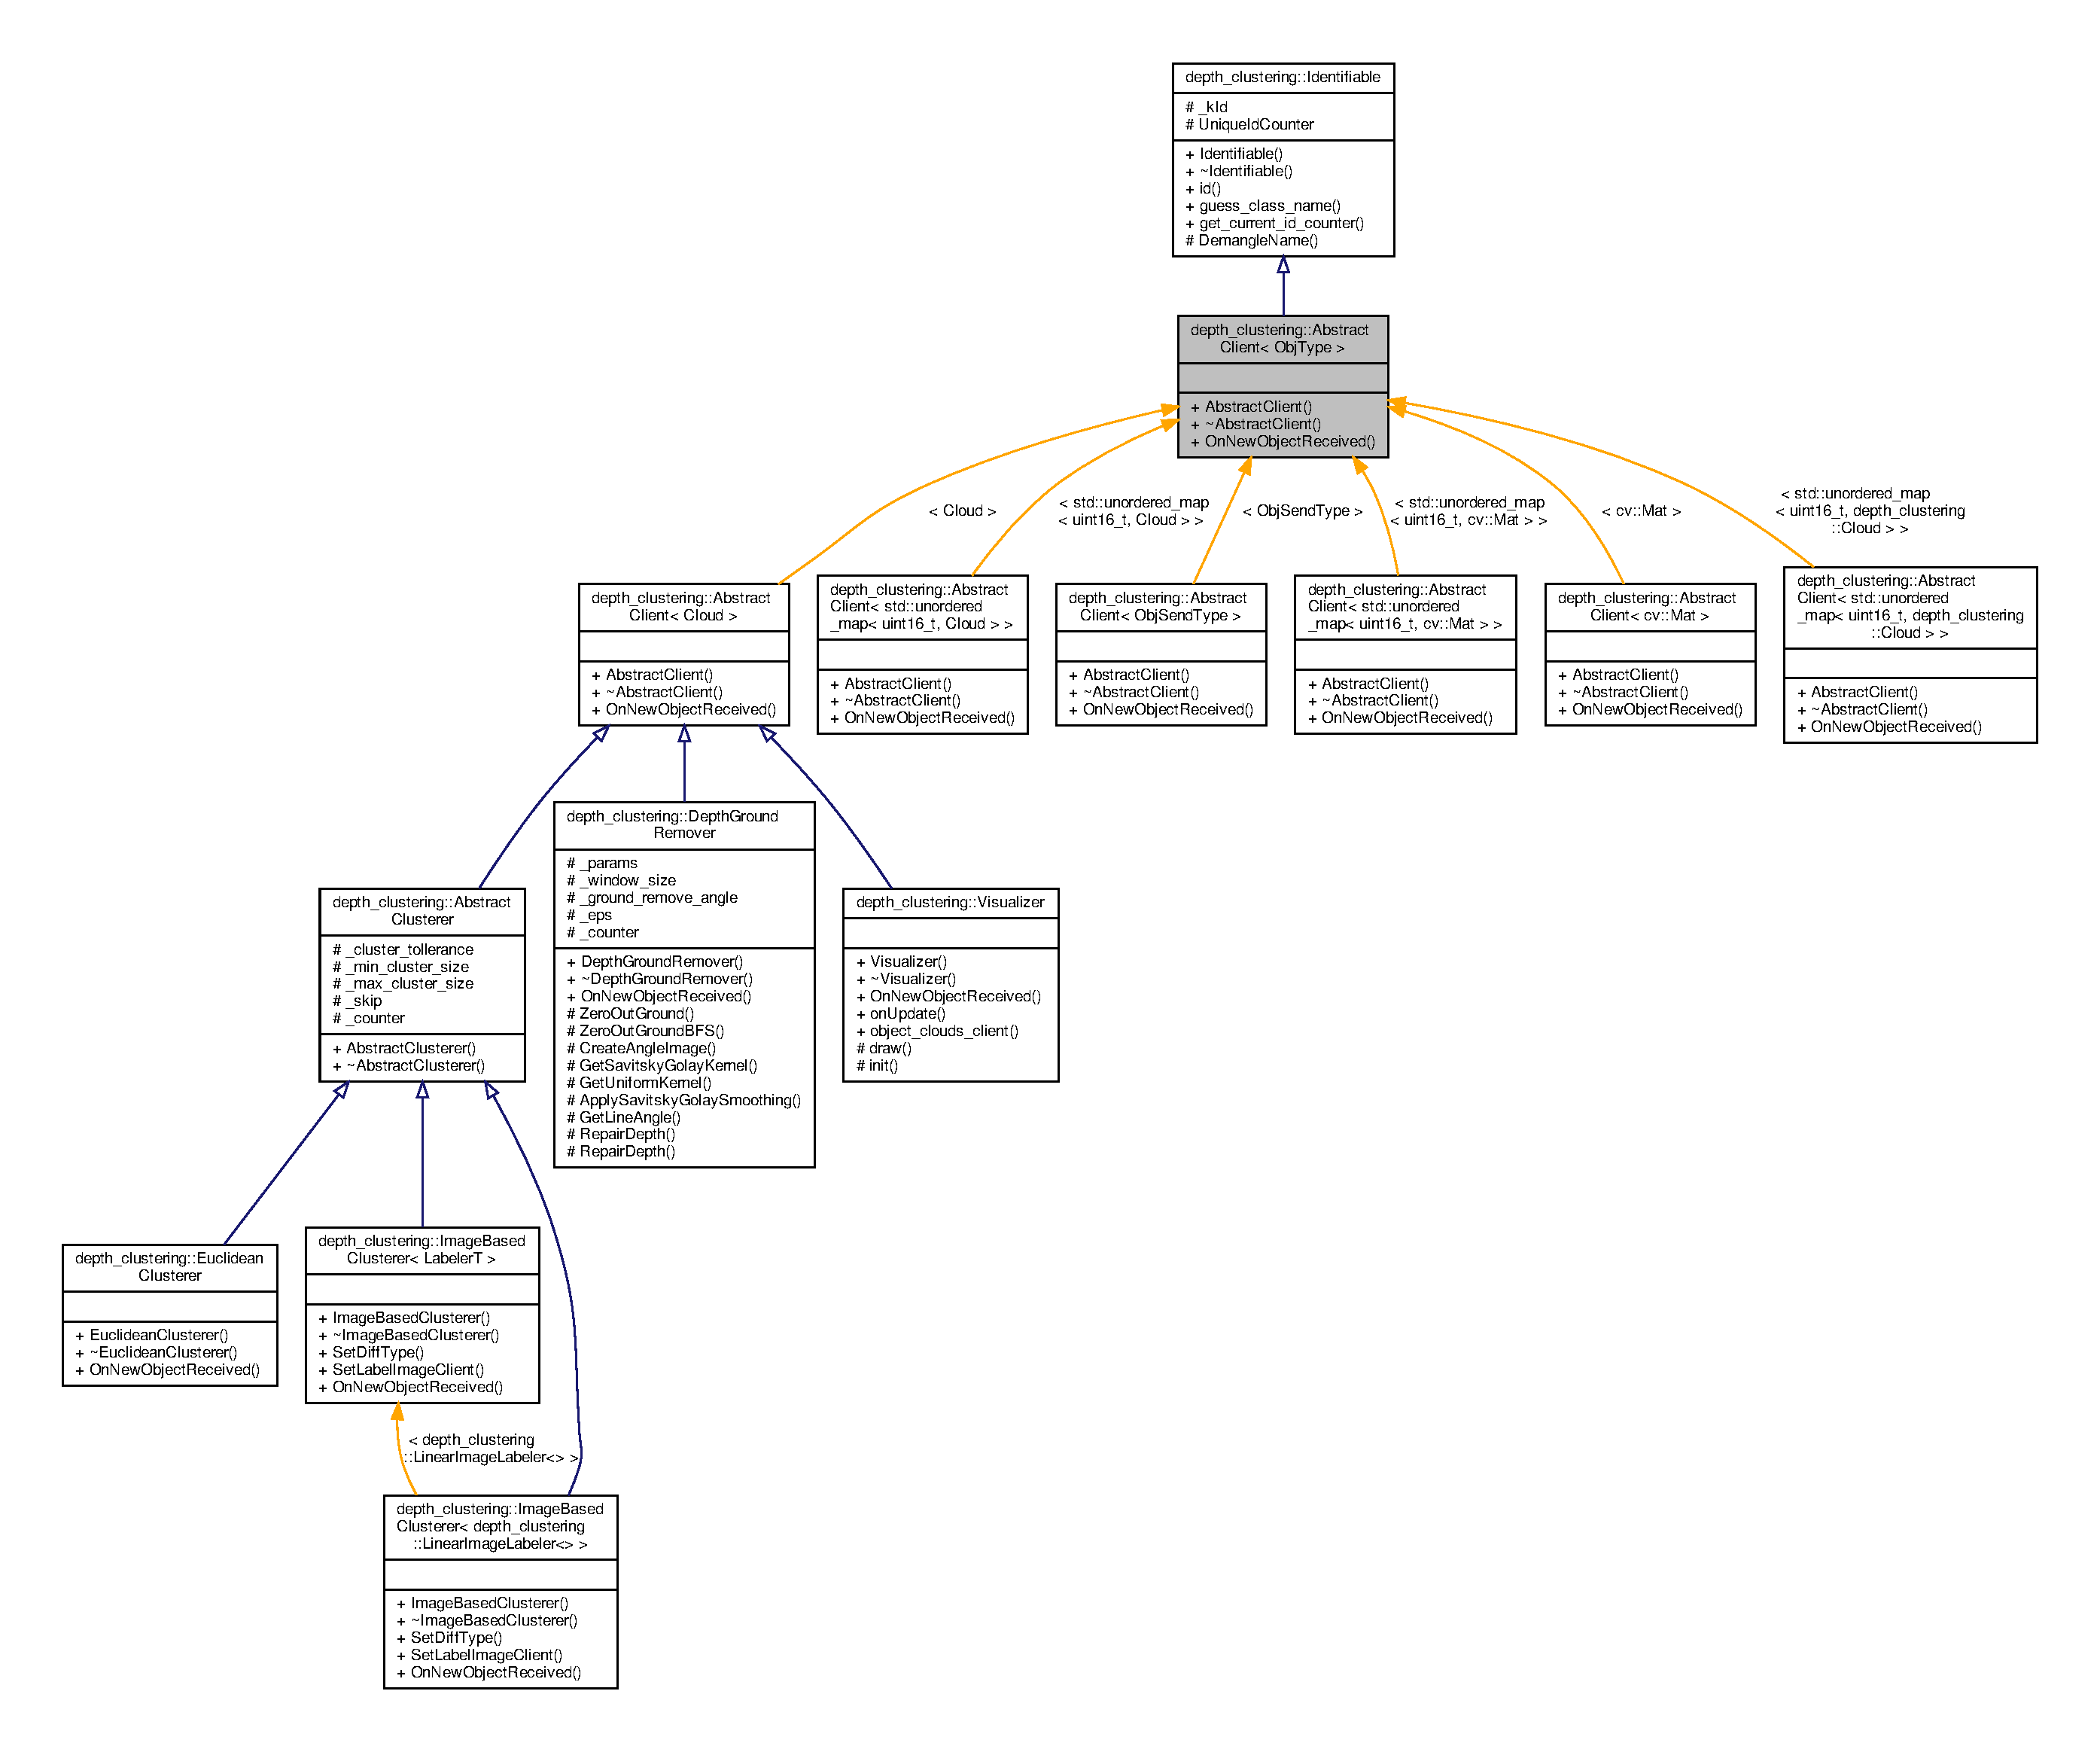
\includegraphics[width=350pt]{classdepth__clustering_1_1AbstractClient__inherit__graph}
\end{center}
\end{figure}


Collaboration diagram for depth\+\_\+clustering\+:\+:Abstract\+Client$<$ Obj\+Type $>$\+:\nopagebreak
\begin{figure}[H]
\begin{center}
\leavevmode
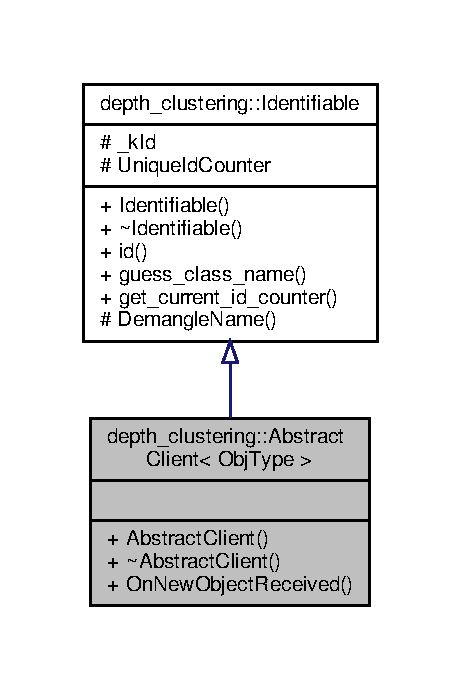
\includegraphics[width=221pt]{classdepth__clustering_1_1AbstractClient__coll__graph}
\end{center}
\end{figure}


The documentation for this class was generated from the following file\+:\begin{DoxyCompactItemize}
\item 
/home/ashwin/catkin\+\_\+ws/src/depth\+\_\+clustering/src/communication/abstract\+\_\+client.\+h\end{DoxyCompactItemize}

\hypertarget{classdepth__clustering_1_1AbstractClusterer}{}\section{depth\+\_\+clustering\+:\+:Abstract\+Clusterer Class Reference}
\label{classdepth__clustering_1_1AbstractClusterer}\index{depth\+\_\+clustering\+::\+Abstract\+Clusterer@{depth\+\_\+clustering\+::\+Abstract\+Clusterer}}


Class for abstract clusterer.  




{\ttfamily \#include $<$abstract\+\_\+clusterer.\+h$>$}

\subsection*{Public Types}
\begin{DoxyCompactItemize}
\item 
\mbox{\Hypertarget{classdepth__clustering_1_1AbstractClusterer_a6417b572cb4d8e851fa5bb88eacfdeb4}\label{classdepth__clustering_1_1AbstractClusterer_a6417b572cb4d8e851fa5bb88eacfdeb4}} 
using {\bfseries Receiver} = \hyperlink{classdepth__clustering_1_1AbstractClient}{Abstract\+Client}$<$ \hyperlink{classdepth__clustering_1_1Cloud}{Cloud} $>$
\item 
\mbox{\Hypertarget{classdepth__clustering_1_1AbstractClusterer_a916148ff0737bb829b47ec704df8e5a4}\label{classdepth__clustering_1_1AbstractClusterer_a916148ff0737bb829b47ec704df8e5a4}} 
using {\bfseries Sender} = \hyperlink{classdepth__clustering_1_1AbstractSender}{Abstract\+Sender}$<$ std\+::unordered\+\_\+map$<$ uint16\+\_\+t, \hyperlink{classdepth__clustering_1_1Cloud}{Cloud} $>$ $>$
\end{DoxyCompactItemize}
\subsection*{Public Member Functions}
\begin{DoxyCompactItemize}
\item 
\hyperlink{classdepth__clustering_1_1AbstractClusterer_a6be8ef3c30066a96e1efa0f082634ed0}{Abstract\+Clusterer} (double cluster\+\_\+tollerance=0.\+2, uint16\+\_\+t min\+\_\+cluster\+\_\+size=100, uint16\+\_\+t max\+\_\+cluster\+\_\+size=25000, uint16\+\_\+t skip=10)
\begin{DoxyCompactList}\small\item\em Construct a clusterer. \end{DoxyCompactList}\end{DoxyCompactItemize}
\subsection*{Protected Attributes}
\begin{DoxyCompactItemize}
\item 
\mbox{\Hypertarget{classdepth__clustering_1_1AbstractClusterer_ae219f21aefc118debe4fc89dfb0af96a}\label{classdepth__clustering_1_1AbstractClusterer_ae219f21aefc118debe4fc89dfb0af96a}} 
double {\bfseries \+\_\+cluster\+\_\+tollerance}
\item 
\mbox{\Hypertarget{classdepth__clustering_1_1AbstractClusterer_a7057f78c03aa9396850a61a92574f502}\label{classdepth__clustering_1_1AbstractClusterer_a7057f78c03aa9396850a61a92574f502}} 
uint16\+\_\+t {\bfseries \+\_\+min\+\_\+cluster\+\_\+size}
\item 
\mbox{\Hypertarget{classdepth__clustering_1_1AbstractClusterer_ad11f0fd4ec9f7b83e9242d6fbbda0661}\label{classdepth__clustering_1_1AbstractClusterer_ad11f0fd4ec9f7b83e9242d6fbbda0661}} 
uint16\+\_\+t {\bfseries \+\_\+max\+\_\+cluster\+\_\+size}
\item 
\mbox{\Hypertarget{classdepth__clustering_1_1AbstractClusterer_a4cc536460eb6ffb1d13cf2eba8039602}\label{classdepth__clustering_1_1AbstractClusterer_a4cc536460eb6ffb1d13cf2eba8039602}} 
uint16\+\_\+t {\bfseries \+\_\+skip}
\item 
\mbox{\Hypertarget{classdepth__clustering_1_1AbstractClusterer_a951128009a13fde1a391289b359cdad2}\label{classdepth__clustering_1_1AbstractClusterer_a951128009a13fde1a391289b359cdad2}} 
uint32\+\_\+t {\bfseries \+\_\+counter}
\end{DoxyCompactItemize}
\subsection*{Additional Inherited Members}


\subsection{Detailed Description}
Class for abstract clusterer. 

Inheritance diagram for depth\+\_\+clustering\+:\+:Abstract\+Clusterer\+:\nopagebreak
\begin{figure}[H]
\begin{center}
\leavevmode
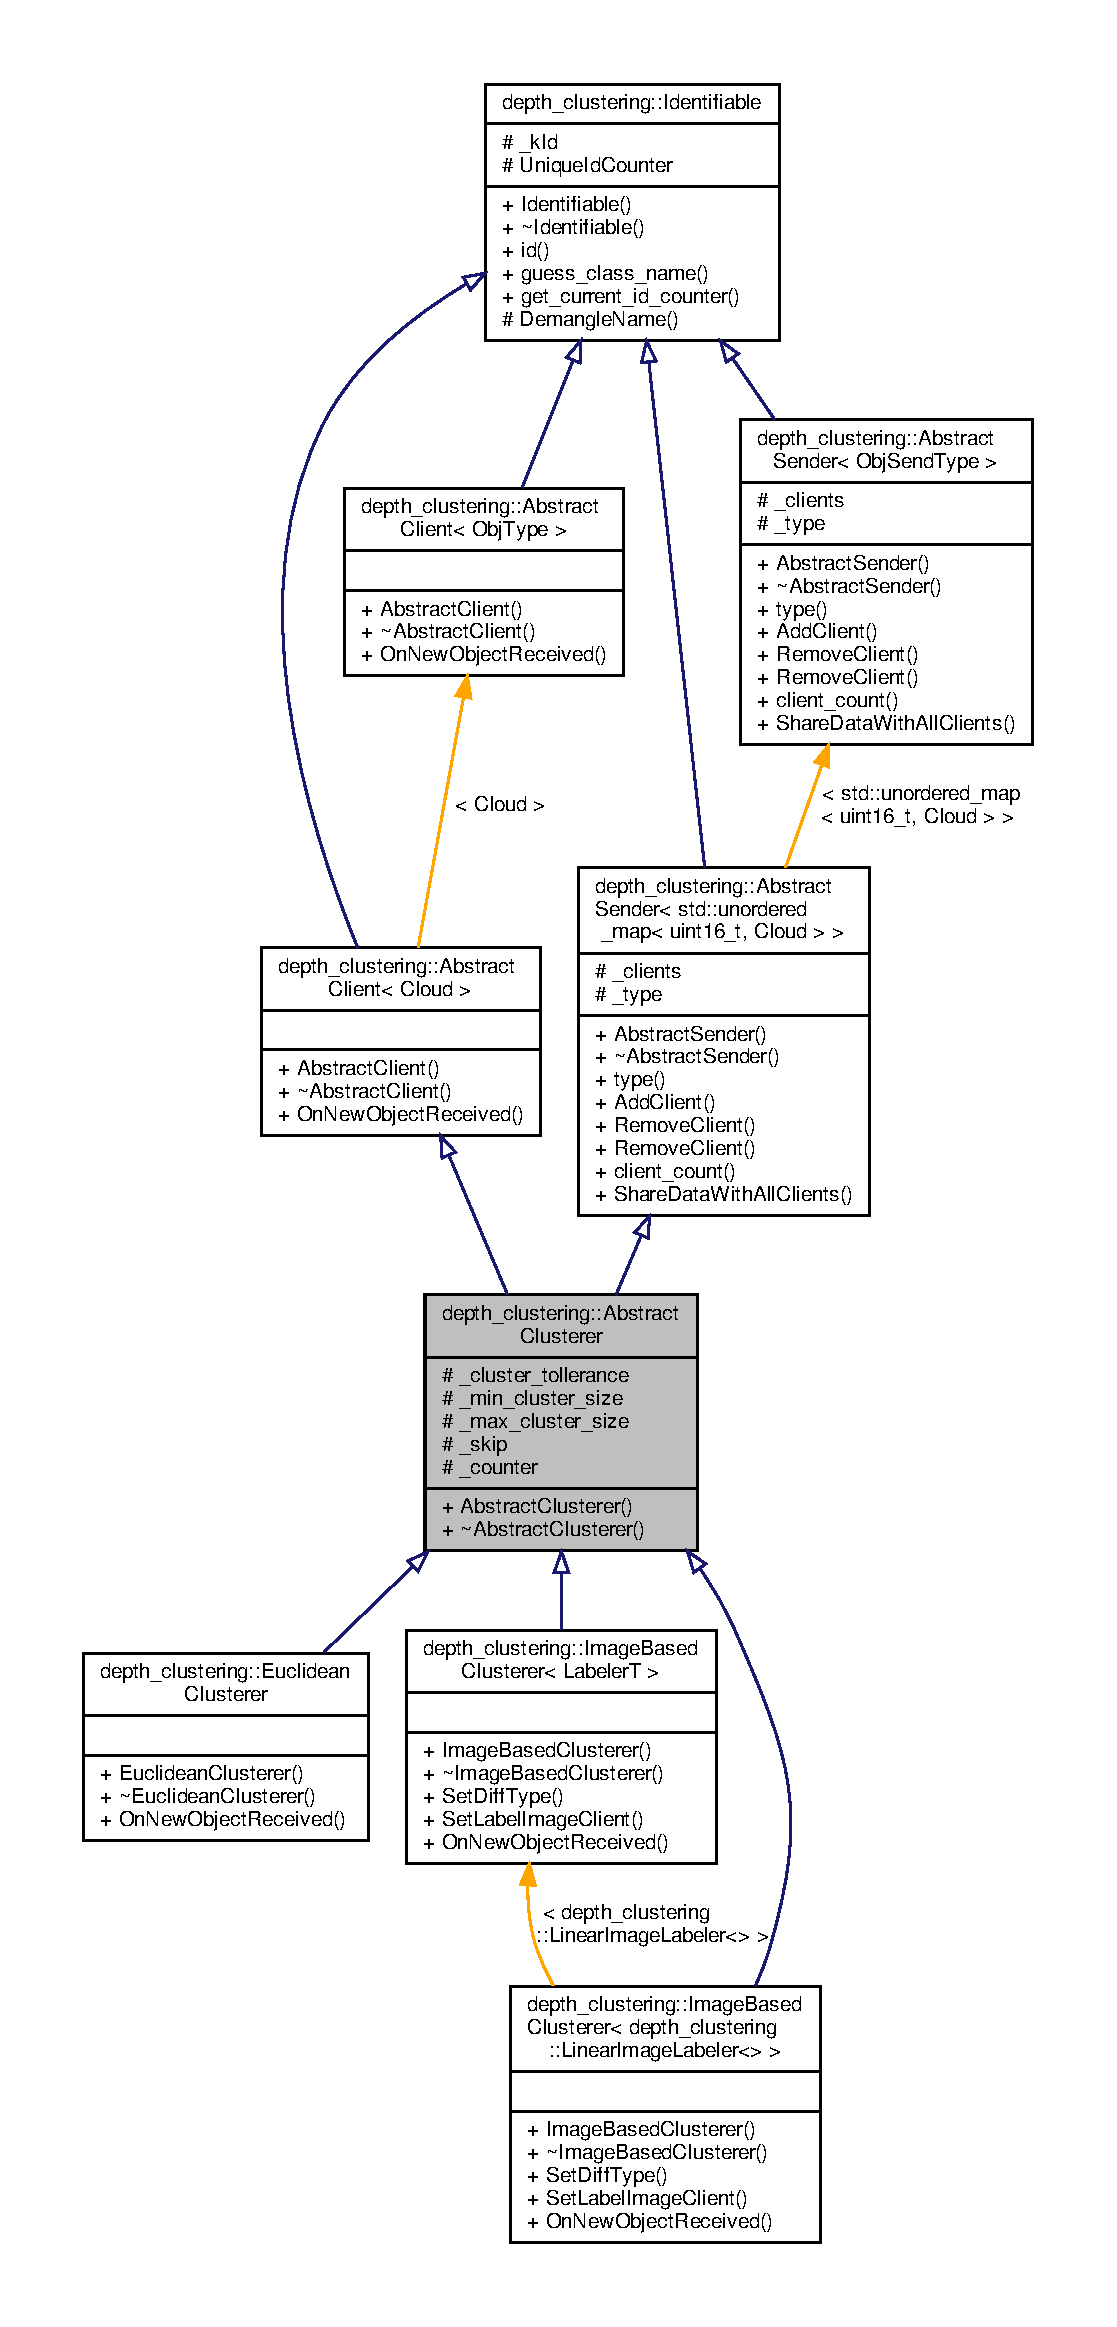
\includegraphics[height=550pt]{classdepth__clustering_1_1AbstractClusterer__inherit__graph}
\end{center}
\end{figure}


Collaboration diagram for depth\+\_\+clustering\+:\+:Abstract\+Clusterer\+:\nopagebreak
\begin{figure}[H]
\begin{center}
\leavevmode
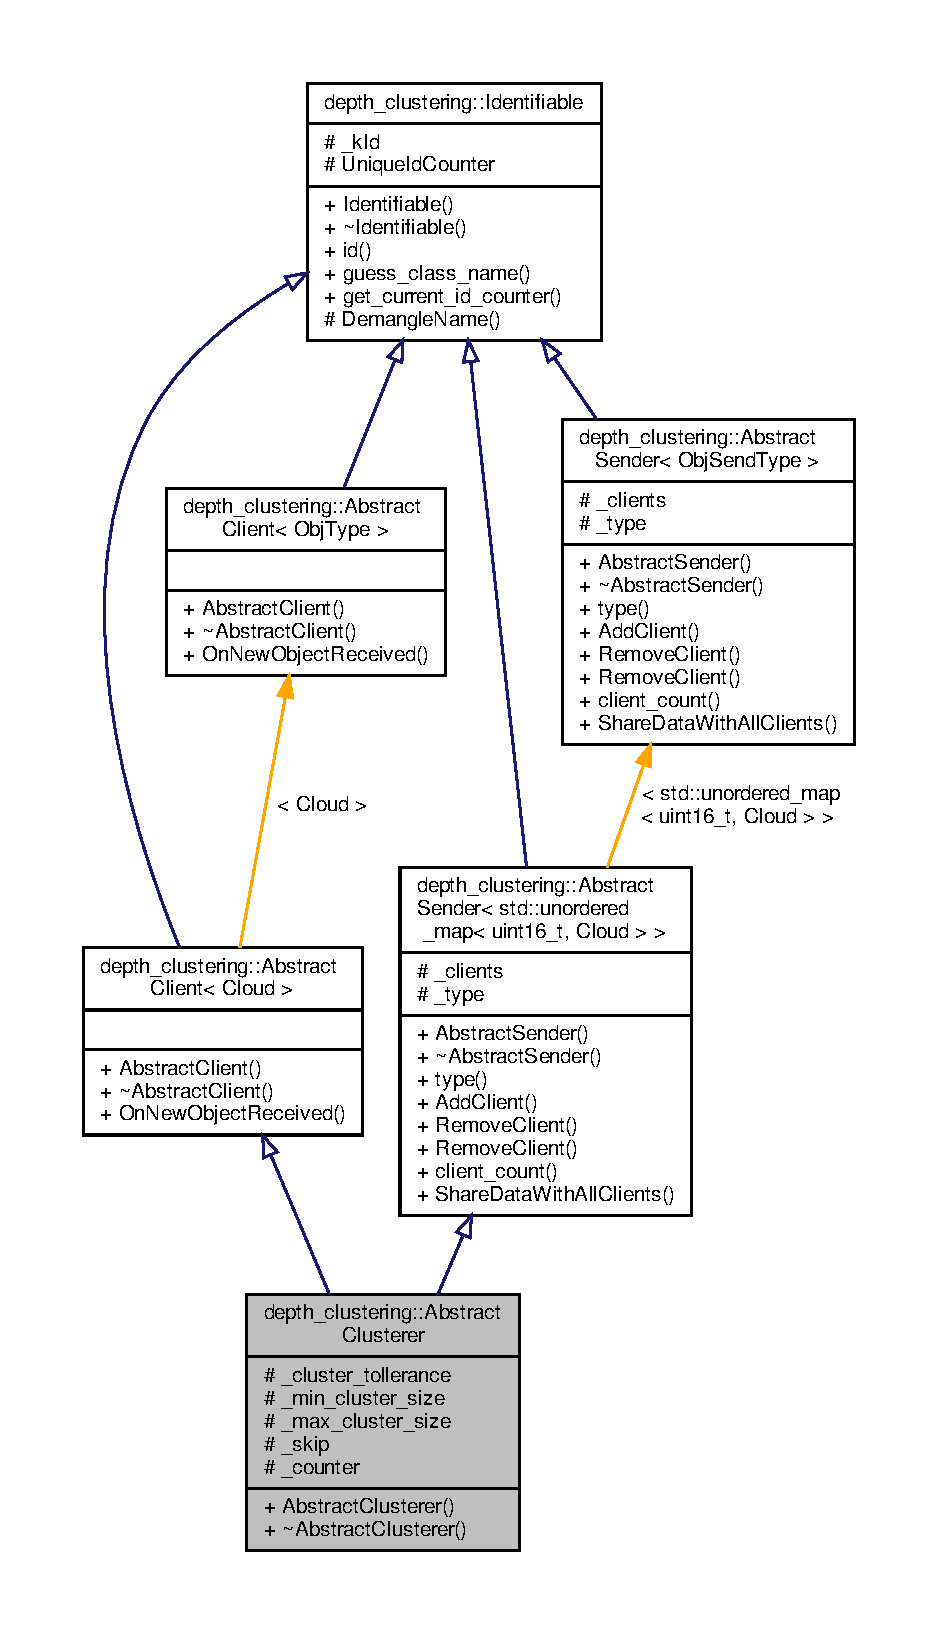
\includegraphics[height=550pt]{classdepth__clustering_1_1AbstractClusterer__coll__graph}
\end{center}
\end{figure}


\subsection{Constructor \& Destructor Documentation}
\mbox{\Hypertarget{classdepth__clustering_1_1AbstractClusterer_a6be8ef3c30066a96e1efa0f082634ed0}\label{classdepth__clustering_1_1AbstractClusterer_a6be8ef3c30066a96e1efa0f082634ed0}} 
\index{depth\+\_\+clustering\+::\+Abstract\+Clusterer@{depth\+\_\+clustering\+::\+Abstract\+Clusterer}!Abstract\+Clusterer@{Abstract\+Clusterer}}
\index{Abstract\+Clusterer@{Abstract\+Clusterer}!depth\+\_\+clustering\+::\+Abstract\+Clusterer@{depth\+\_\+clustering\+::\+Abstract\+Clusterer}}
\subsubsection{\texorpdfstring{Abstract\+Clusterer()}{AbstractClusterer()}}
{\footnotesize\ttfamily depth\+\_\+clustering\+::\+Abstract\+Clusterer\+::\+Abstract\+Clusterer (\begin{DoxyParamCaption}\item[{double}]{cluster\+\_\+tollerance = {\ttfamily 0.2},  }\item[{uint16\+\_\+t}]{min\+\_\+cluster\+\_\+size = {\ttfamily 100},  }\item[{uint16\+\_\+t}]{max\+\_\+cluster\+\_\+size = {\ttfamily 25000},  }\item[{uint16\+\_\+t}]{skip = {\ttfamily 10} }\end{DoxyParamCaption})\hspace{0.3cm}{\ttfamily [inline]}, {\ttfamily [explicit]}}



Construct a clusterer. 


\begin{DoxyParams}[1]{Parameters}
\mbox{\tt in}  & {\em cluster\+\_\+tollerance} & The cluster tollerance \\
\hline
\mbox{\tt in}  & {\em min\+\_\+cluster\+\_\+size} & The minimum cluster size \\
\hline
\mbox{\tt in}  & {\em max\+\_\+cluster\+\_\+size} & The maximum cluster size \\
\hline
\mbox{\tt in}  & {\em skip} & Only cluster every skip cloud \\
\hline
\end{DoxyParams}


The documentation for this class was generated from the following file\+:\begin{DoxyCompactItemize}
\item 
/home/ashwin/catkin\+\_\+ws/src/depth\+\_\+clustering/src/clusterers/abstract\+\_\+clusterer.\+h\end{DoxyCompactItemize}

\hypertarget{classdepth__clustering_1_1AbstractDiff}{}\section{depth\+\_\+clustering\+:\+:Abstract\+Diff Class Reference}
\label{classdepth__clustering_1_1AbstractDiff}\index{depth\+\_\+clustering\+::\+Abstract\+Diff@{depth\+\_\+clustering\+::\+Abstract\+Diff}}


Class for abstract difference.  




{\ttfamily \#include $<$abstract\+\_\+diff.\+h$>$}

\subsection*{Public Member Functions}
\begin{DoxyCompactItemize}
\item 
\hyperlink{classdepth__clustering_1_1AbstractDiff_a14160500db5c2c1c1948a9e563318cc8}{Abstract\+Diff} (const cv\+::\+Mat $\ast$source\+\_\+image)
\begin{DoxyCompactList}\small\item\em construct a class with a source image pointer \end{DoxyCompactList}\item 
virtual float \hyperlink{classdepth__clustering_1_1AbstractDiff_a06ba188d8d83d0e4bad66c833656c26d}{Diff\+At} (const \hyperlink{structdepth__clustering_1_1PixelCoord}{Pixel\+Coord} \&from, const \hyperlink{structdepth__clustering_1_1PixelCoord}{Pixel\+Coord} \&to) const =0
\begin{DoxyCompactList}\small\item\em Gets diff between pixels from and to. \end{DoxyCompactList}\item 
virtual bool \hyperlink{classdepth__clustering_1_1AbstractDiff_a940280569ed86d8f7e95626b1a2312d7}{Satisfies\+Threshold} (float value, float threshold) const =0
\begin{DoxyCompactList}\small\item\em Does the difference satisfy a threshold? \end{DoxyCompactList}\item 
virtual cv\+::\+Mat \hyperlink{classdepth__clustering_1_1AbstractDiff_a45314bf711f35e53590af28bdfc45313}{Visualize} () const
\begin{DoxyCompactList}\small\item\em Visualize the differences as a color image. \end{DoxyCompactList}\end{DoxyCompactItemize}
\subsection*{Protected Attributes}
\begin{DoxyCompactItemize}
\item 
\mbox{\Hypertarget{classdepth__clustering_1_1AbstractDiff_ac554e78b6f29341d1361a8ec6932698a}\label{classdepth__clustering_1_1AbstractDiff_ac554e78b6f29341d1361a8ec6932698a}} 
const cv\+::\+Mat $\ast$ {\bfseries \+\_\+source\+\_\+image} = nullptr
\end{DoxyCompactItemize}


\subsection{Detailed Description}
Class for abstract difference. 

Inheritance diagram for depth\+\_\+clustering\+:\+:Abstract\+Diff\+:\nopagebreak
\begin{figure}[H]
\begin{center}
\leavevmode
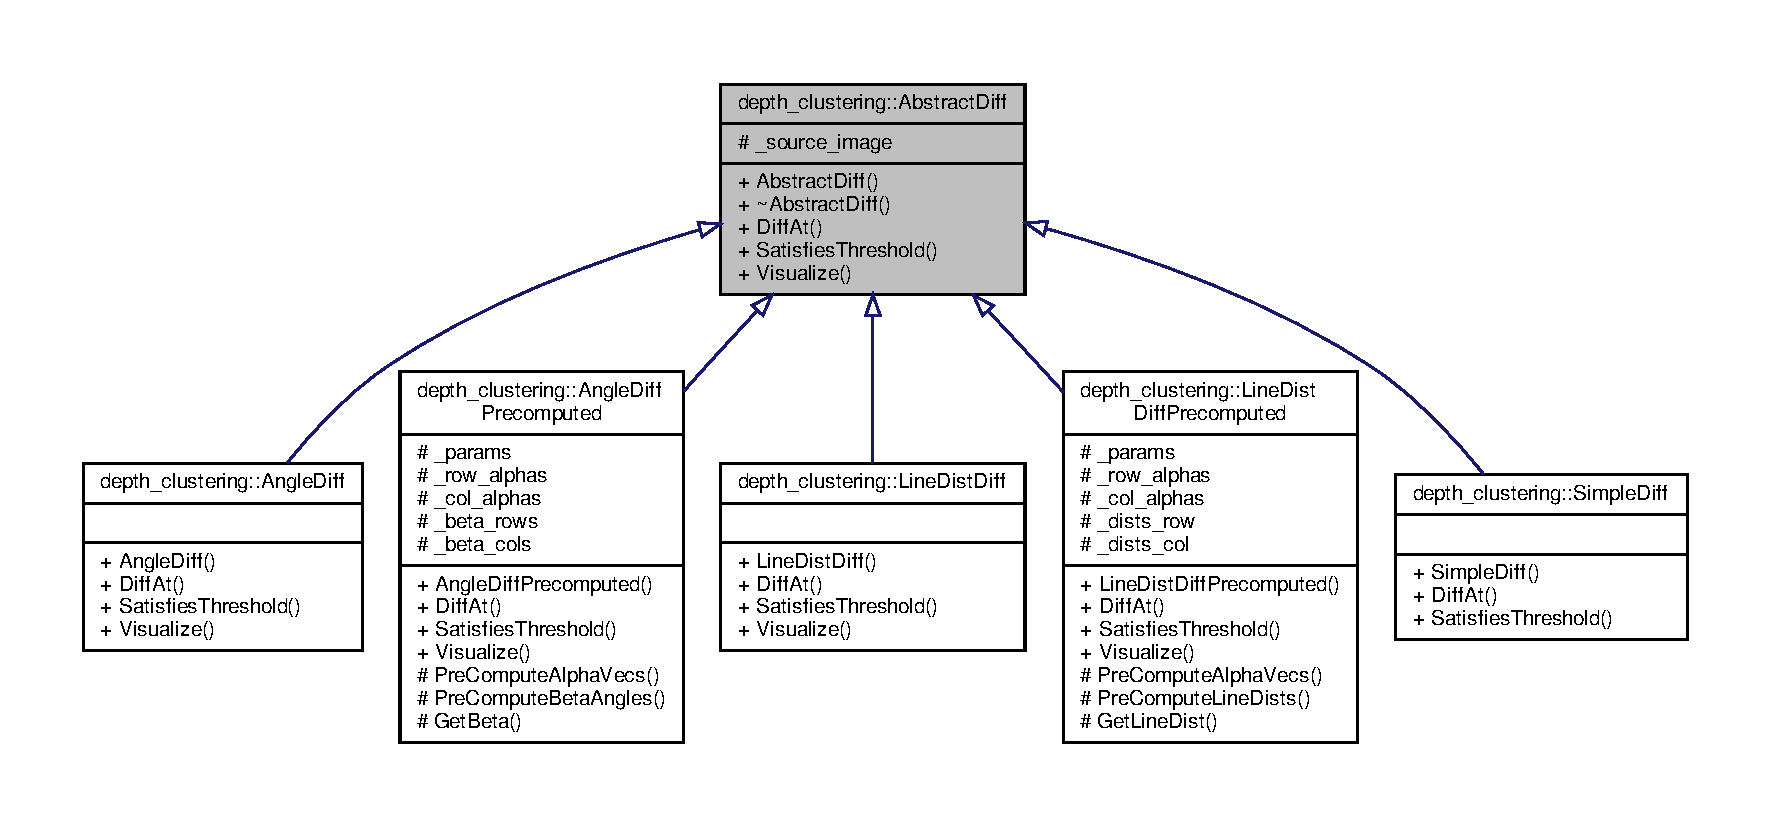
\includegraphics[width=350pt]{classdepth__clustering_1_1AbstractDiff__inherit__graph}
\end{center}
\end{figure}


Collaboration diagram for depth\+\_\+clustering\+:\+:Abstract\+Diff\+:\nopagebreak
\begin{figure}[H]
\begin{center}
\leavevmode
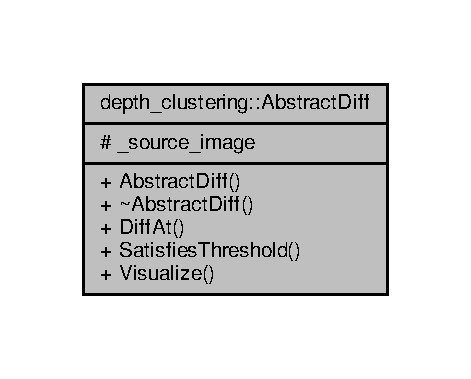
\includegraphics[width=226pt]{classdepth__clustering_1_1AbstractDiff__coll__graph}
\end{center}
\end{figure}


\subsection{Constructor \& Destructor Documentation}
\mbox{\Hypertarget{classdepth__clustering_1_1AbstractDiff_a14160500db5c2c1c1948a9e563318cc8}\label{classdepth__clustering_1_1AbstractDiff_a14160500db5c2c1c1948a9e563318cc8}} 
\index{depth\+\_\+clustering\+::\+Abstract\+Diff@{depth\+\_\+clustering\+::\+Abstract\+Diff}!Abstract\+Diff@{Abstract\+Diff}}
\index{Abstract\+Diff@{Abstract\+Diff}!depth\+\_\+clustering\+::\+Abstract\+Diff@{depth\+\_\+clustering\+::\+Abstract\+Diff}}
\subsubsection{\texorpdfstring{Abstract\+Diff()}{AbstractDiff()}}
{\footnotesize\ttfamily depth\+\_\+clustering\+::\+Abstract\+Diff\+::\+Abstract\+Diff (\begin{DoxyParamCaption}\item[{const cv\+::\+Mat $\ast$}]{source\+\_\+image }\end{DoxyParamCaption})\hspace{0.3cm}{\ttfamily [inline]}, {\ttfamily [explicit]}}



construct a class with a source image pointer 


\begin{DoxyParams}[1]{Parameters}
\mbox{\tt in}  & {\em source\+\_\+image} & The source image pointer (C\+V\+\_\+32F type Mat) \\
\hline
\end{DoxyParams}
Here is the call graph for this function\+:\nopagebreak
\begin{figure}[H]
\begin{center}
\leavevmode
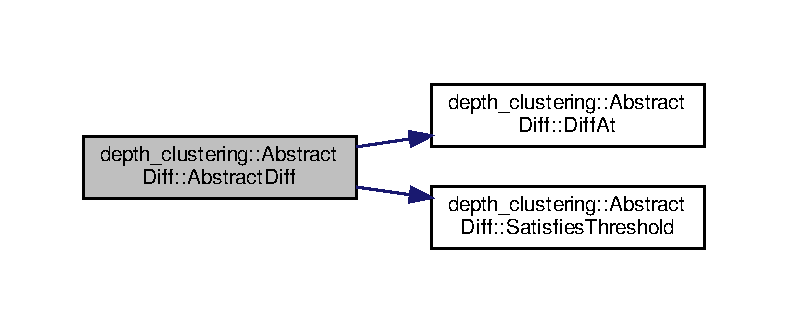
\includegraphics[width=350pt]{classdepth__clustering_1_1AbstractDiff_a14160500db5c2c1c1948a9e563318cc8_cgraph}
\end{center}
\end{figure}


\subsection{Member Function Documentation}
\mbox{\Hypertarget{classdepth__clustering_1_1AbstractDiff_a06ba188d8d83d0e4bad66c833656c26d}\label{classdepth__clustering_1_1AbstractDiff_a06ba188d8d83d0e4bad66c833656c26d}} 
\index{depth\+\_\+clustering\+::\+Abstract\+Diff@{depth\+\_\+clustering\+::\+Abstract\+Diff}!Diff\+At@{Diff\+At}}
\index{Diff\+At@{Diff\+At}!depth\+\_\+clustering\+::\+Abstract\+Diff@{depth\+\_\+clustering\+::\+Abstract\+Diff}}
\subsubsection{\texorpdfstring{Diff\+At()}{DiffAt()}}
{\footnotesize\ttfamily virtual float depth\+\_\+clustering\+::\+Abstract\+Diff\+::\+Diff\+At (\begin{DoxyParamCaption}\item[{const \hyperlink{structdepth__clustering_1_1PixelCoord}{Pixel\+Coord} \&}]{from,  }\item[{const \hyperlink{structdepth__clustering_1_1PixelCoord}{Pixel\+Coord} \&}]{to }\end{DoxyParamCaption}) const\hspace{0.3cm}{\ttfamily [pure virtual]}}



Gets diff between pixels from and to. 


\begin{DoxyParams}[1]{Parameters}
\mbox{\tt in}  & {\em from} & pixel from which we want difference \\
\hline
\mbox{\tt in}  & {\em to} & pixel to which we want difference\\
\hline
\end{DoxyParams}
\begin{DoxyReturn}{Returns}
difference between the pixels 
\end{DoxyReturn}


Implemented in \hyperlink{classdepth__clustering_1_1LineDistDiffPrecomputed_ac505afaa537656af1bcc342ab1e910c4}{depth\+\_\+clustering\+::\+Line\+Dist\+Diff\+Precomputed}, \hyperlink{classdepth__clustering_1_1AngleDiffPrecomputed_ae15bb5fc9488ae2b26c77665931b8626}{depth\+\_\+clustering\+::\+Angle\+Diff\+Precomputed}, \hyperlink{classdepth__clustering_1_1LineDistDiff_a839eee44b14de26d85e6dbad5e37b356}{depth\+\_\+clustering\+::\+Line\+Dist\+Diff}, \hyperlink{classdepth__clustering_1_1AngleDiff_ac9bd0ec61ff0b213fd19235dc171c1c2}{depth\+\_\+clustering\+::\+Angle\+Diff}, and \hyperlink{classdepth__clustering_1_1SimpleDiff_a3afe28bd6a9cfbaff18e856a04d24824}{depth\+\_\+clustering\+::\+Simple\+Diff}.

Here is the caller graph for this function\+:\nopagebreak
\begin{figure}[H]
\begin{center}
\leavevmode
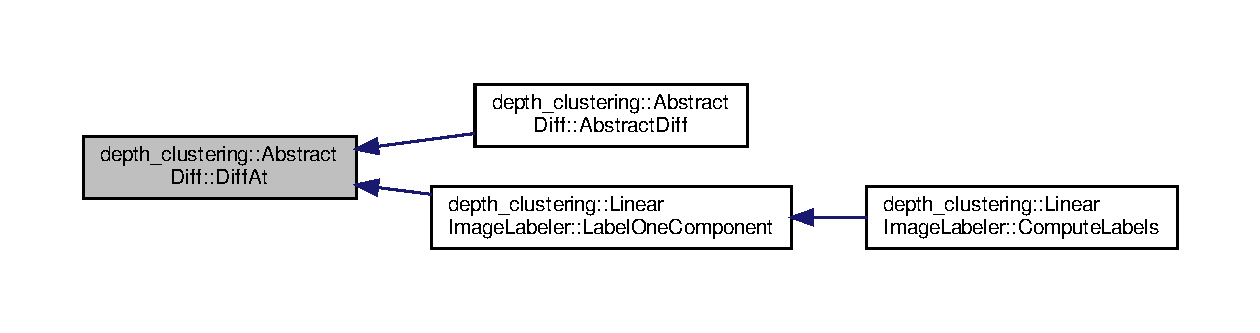
\includegraphics[width=350pt]{classdepth__clustering_1_1AbstractDiff_a06ba188d8d83d0e4bad66c833656c26d_icgraph}
\end{center}
\end{figure}
\mbox{\Hypertarget{classdepth__clustering_1_1AbstractDiff_a940280569ed86d8f7e95626b1a2312d7}\label{classdepth__clustering_1_1AbstractDiff_a940280569ed86d8f7e95626b1a2312d7}} 
\index{depth\+\_\+clustering\+::\+Abstract\+Diff@{depth\+\_\+clustering\+::\+Abstract\+Diff}!Satisfies\+Threshold@{Satisfies\+Threshold}}
\index{Satisfies\+Threshold@{Satisfies\+Threshold}!depth\+\_\+clustering\+::\+Abstract\+Diff@{depth\+\_\+clustering\+::\+Abstract\+Diff}}
\subsubsection{\texorpdfstring{Satisfies\+Threshold()}{SatisfiesThreshold()}}
{\footnotesize\ttfamily virtual bool depth\+\_\+clustering\+::\+Abstract\+Diff\+::\+Satisfies\+Threshold (\begin{DoxyParamCaption}\item[{float}]{value,  }\item[{float}]{threshold }\end{DoxyParamCaption}) const\hspace{0.3cm}{\ttfamily [pure virtual]}}



Does the difference satisfy a threshold? 


\begin{DoxyParams}[1]{Parameters}
\mbox{\tt in}  & {\em value} & Query value \\
\hline
\mbox{\tt in}  & {\em threshold} & The threshold\\
\hline
\end{DoxyParams}
\begin{DoxyReturn}{Returns}
true if satisfies, false, otherwise 
\end{DoxyReturn}


Implemented in \hyperlink{classdepth__clustering_1_1LineDistDiffPrecomputed_ac3ce8196d5e6f49f3e3bdc3e3b32b033}{depth\+\_\+clustering\+::\+Line\+Dist\+Diff\+Precomputed}, \hyperlink{classdepth__clustering_1_1AngleDiffPrecomputed_a28a32c0cb0405163fe237909fe5f6c0c}{depth\+\_\+clustering\+::\+Angle\+Diff\+Precomputed}, \hyperlink{classdepth__clustering_1_1LineDistDiff_ae9debede2cffd6bb40ca4c4a82c52f61}{depth\+\_\+clustering\+::\+Line\+Dist\+Diff}, \hyperlink{classdepth__clustering_1_1AngleDiff_ac65e8f42b1f2ac82db14ebe188c004a2}{depth\+\_\+clustering\+::\+Angle\+Diff}, and \hyperlink{classdepth__clustering_1_1SimpleDiff_a277c862d4ffdf1bfc24bd1bd70cb98a7}{depth\+\_\+clustering\+::\+Simple\+Diff}.

Here is the caller graph for this function\+:\nopagebreak
\begin{figure}[H]
\begin{center}
\leavevmode
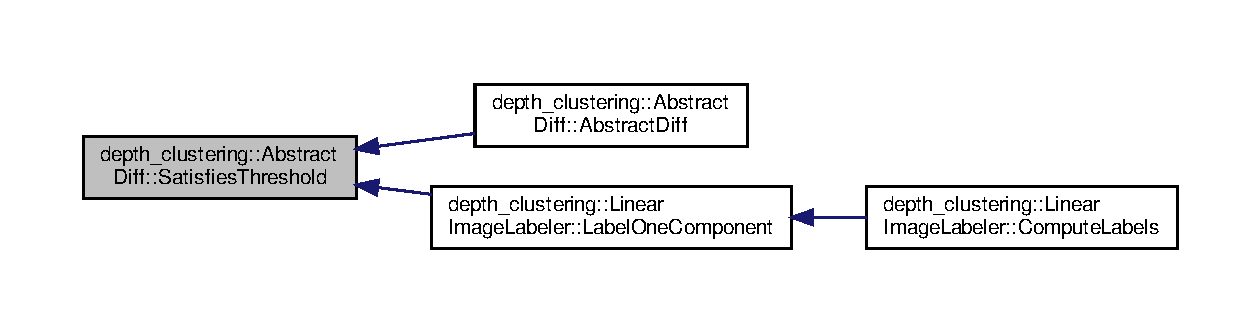
\includegraphics[width=350pt]{classdepth__clustering_1_1AbstractDiff_a940280569ed86d8f7e95626b1a2312d7_icgraph}
\end{center}
\end{figure}
\mbox{\Hypertarget{classdepth__clustering_1_1AbstractDiff_a45314bf711f35e53590af28bdfc45313}\label{classdepth__clustering_1_1AbstractDiff_a45314bf711f35e53590af28bdfc45313}} 
\index{depth\+\_\+clustering\+::\+Abstract\+Diff@{depth\+\_\+clustering\+::\+Abstract\+Diff}!Visualize@{Visualize}}
\index{Visualize@{Visualize}!depth\+\_\+clustering\+::\+Abstract\+Diff@{depth\+\_\+clustering\+::\+Abstract\+Diff}}
\subsubsection{\texorpdfstring{Visualize()}{Visualize()}}
{\footnotesize\ttfamily virtual cv\+::\+Mat depth\+\_\+clustering\+::\+Abstract\+Diff\+::\+Visualize (\begin{DoxyParamCaption}{ }\end{DoxyParamCaption}) const\hspace{0.3cm}{\ttfamily [inline]}, {\ttfamily [virtual]}}



Visualize the differences as a color image. 

\begin{DoxyReturn}{Returns}
Open\+CV Mat of type C\+V\+\_\+8\+U\+C3 to visualize differences in color. 
\end{DoxyReturn}


Reimplemented in \hyperlink{classdepth__clustering_1_1LineDistDiffPrecomputed_a77c9cf3bea954f13cd2fef4f8a182425}{depth\+\_\+clustering\+::\+Line\+Dist\+Diff\+Precomputed}, \hyperlink{classdepth__clustering_1_1AngleDiffPrecomputed_a2fd85404d06843af0ee5c713017f6641}{depth\+\_\+clustering\+::\+Angle\+Diff\+Precomputed}, \hyperlink{classdepth__clustering_1_1LineDistDiff_a7feaf820589ccfb47786d5124a74d725}{depth\+\_\+clustering\+::\+Line\+Dist\+Diff}, and \hyperlink{classdepth__clustering_1_1AngleDiff_a462e4aadd35ca06e9b061d08c9787074}{depth\+\_\+clustering\+::\+Angle\+Diff}.



The documentation for this class was generated from the following file\+:\begin{DoxyCompactItemize}
\item 
/home/ashwin/catkin\+\_\+ws/src/depth\+\_\+clustering/src/image\+\_\+labelers/diff\+\_\+helpers/abstract\+\_\+diff.\+h\end{DoxyCompactItemize}

\hypertarget{classdepth__clustering_1_1AbstractImageLabeler}{}\section{depth\+\_\+clustering\+:\+:Abstract\+Image\+Labeler Class Reference}
\label{classdepth__clustering_1_1AbstractImageLabeler}\index{depth\+\_\+clustering\+::\+Abstract\+Image\+Labeler@{depth\+\_\+clustering\+::\+Abstract\+Image\+Labeler}}


Class for abstract image labeler.  




{\ttfamily \#include $<$abstract\+\_\+image\+\_\+labeler.\+h$>$}

\subsection*{Public Member Functions}
\begin{DoxyCompactItemize}
\item 
\mbox{\Hypertarget{classdepth__clustering_1_1AbstractImageLabeler_ac01889e0a3d088cf7627809f4d8aab19}\label{classdepth__clustering_1_1AbstractImageLabeler_ac01889e0a3d088cf7627809f4d8aab19}} 
{\bfseries Abstract\+Image\+Labeler} (const cv\+::\+Mat \&depth\+\_\+image, const \hyperlink{classdepth__clustering_1_1ProjectionParams}{Projection\+Params} \&params, const Radians \&angle\+\_\+threshold)
\item 
\mbox{\Hypertarget{classdepth__clustering_1_1AbstractImageLabeler_a28e8e094c9a47a02a2ce9eabef9526e6}\label{classdepth__clustering_1_1AbstractImageLabeler_a28e8e094c9a47a02a2ce9eabef9526e6}} 
void {\bfseries Set\+Depth\+Image} (const cv\+::\+Mat \&depth\+\_\+image)
\item 
\mbox{\Hypertarget{classdepth__clustering_1_1AbstractImageLabeler_ac66f0554e1c988ab0bf413a2f17d3905}\label{classdepth__clustering_1_1AbstractImageLabeler_ac66f0554e1c988ab0bf413a2f17d3905}} 
virtual void \hyperlink{classdepth__clustering_1_1AbstractImageLabeler_ac66f0554e1c988ab0bf413a2f17d3905}{Compute\+Labels} (Diff\+Factory\+::\+Diff\+Type diff\+\_\+type)=0
\begin{DoxyCompactList}\small\item\em An interface for children to compute labels. \end{DoxyCompactList}\item 
const cv\+::\+Mat $\ast$ \hyperlink{classdepth__clustering_1_1AbstractImageLabeler_a7b2f8edf44f3ccb01fb71c296241615e}{Get\+Label\+Image} () const
\begin{DoxyCompactList}\small\item\em Gets the label image. \end{DoxyCompactList}\end{DoxyCompactItemize}
\subsection*{Static Public Member Functions}
\begin{DoxyCompactItemize}
\item 
static cv\+::\+Mat \hyperlink{classdepth__clustering_1_1AbstractImageLabeler_abab18e0c1ca40b54922a2f21948b996b}{Labels\+To\+Color} (const cv\+::\+Mat \&label\+\_\+image)
\begin{DoxyCompactList}\small\item\em Generates random-\/colored image from image of labels. \end{DoxyCompactList}\end{DoxyCompactItemize}
\subsection*{Protected Attributes}
\begin{DoxyCompactItemize}
\item 
\mbox{\Hypertarget{classdepth__clustering_1_1AbstractImageLabeler_adb50d2beeba4e4eac26b5ace9304728b}\label{classdepth__clustering_1_1AbstractImageLabeler_adb50d2beeba4e4eac26b5ace9304728b}} 
const cv\+::\+Mat $\ast$ {\bfseries \+\_\+depth\+\_\+image\+\_\+ptr}
\item 
\mbox{\Hypertarget{classdepth__clustering_1_1AbstractImageLabeler_a25fcaead9f8806fa75ad44c669e2a518}\label{classdepth__clustering_1_1AbstractImageLabeler_a25fcaead9f8806fa75ad44c669e2a518}} 
\hyperlink{classdepth__clustering_1_1ProjectionParams}{Projection\+Params} {\bfseries \+\_\+params}
\item 
\mbox{\Hypertarget{classdepth__clustering_1_1AbstractImageLabeler_aeabb8ac8238c684066f8c0edcca9b807}\label{classdepth__clustering_1_1AbstractImageLabeler_aeabb8ac8238c684066f8c0edcca9b807}} 
cv\+::\+Mat {\bfseries \+\_\+label\+\_\+image}
\item 
\mbox{\Hypertarget{classdepth__clustering_1_1AbstractImageLabeler_a1a338d254a41ba94bd4122aa006fbe57}\label{classdepth__clustering_1_1AbstractImageLabeler_a1a338d254a41ba94bd4122aa006fbe57}} 
float {\bfseries \+\_\+radians\+\_\+threshold}
\end{DoxyCompactItemize}
\subsection*{Static Protected Attributes}
\begin{DoxyCompactItemize}
\item 
\mbox{\Hypertarget{classdepth__clustering_1_1AbstractImageLabeler_a24ea9d1c40b872189a9e93f369ae34b2}\label{classdepth__clustering_1_1AbstractImageLabeler_a24ea9d1c40b872189a9e93f369ae34b2}} 
static constexpr std\+::array$<$ std\+::array$<$ int, 3 $>$, 200 $>$ {\bfseries R\+A\+N\+D\+O\+M\+\_\+\+C\+O\+L\+O\+RS}
\end{DoxyCompactItemize}


\subsection{Detailed Description}
Class for abstract image labeler. 

This class is responsible for labeling an given depth image based on the provided angle\+\_\+threshold. 

Inheritance diagram for depth\+\_\+clustering\+:\+:Abstract\+Image\+Labeler\+:\nopagebreak
\begin{figure}[H]
\begin{center}
\leavevmode
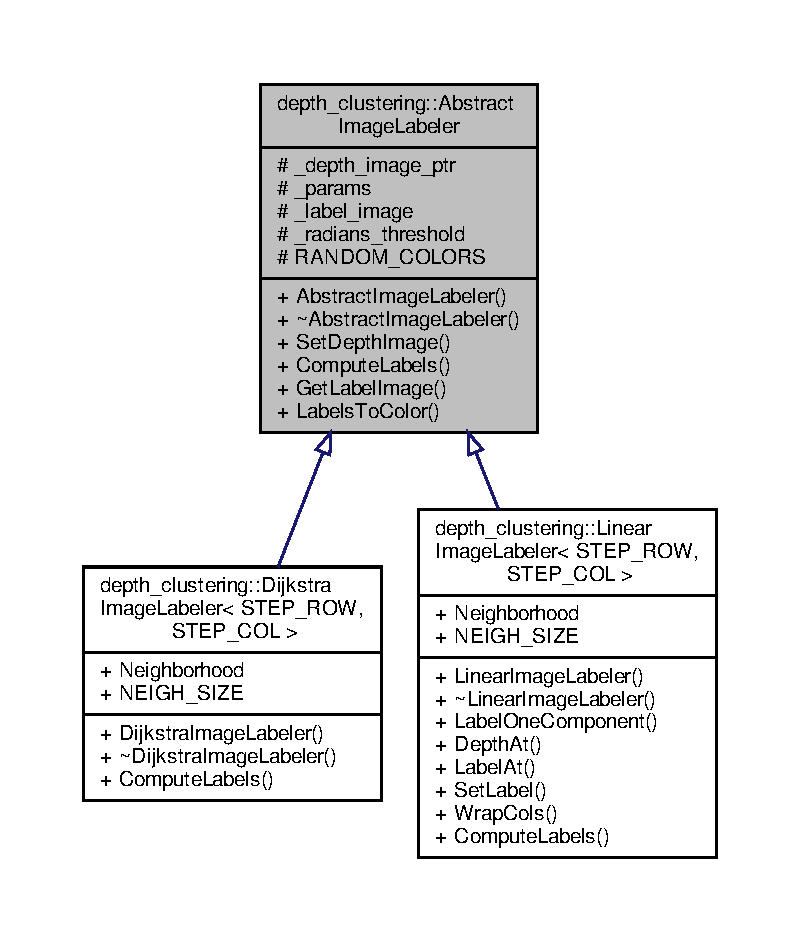
\includegraphics[width=350pt]{classdepth__clustering_1_1AbstractImageLabeler__inherit__graph}
\end{center}
\end{figure}


Collaboration diagram for depth\+\_\+clustering\+:\+:Abstract\+Image\+Labeler\+:\nopagebreak
\begin{figure}[H]
\begin{center}
\leavevmode
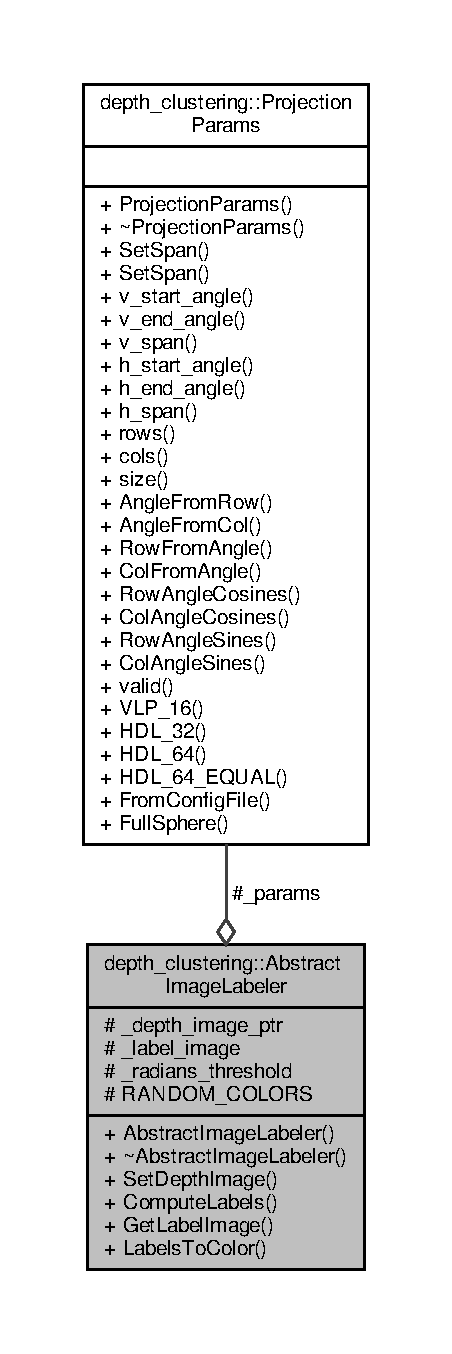
\includegraphics[height=550pt]{classdepth__clustering_1_1AbstractImageLabeler__coll__graph}
\end{center}
\end{figure}


\subsection{Member Function Documentation}
\mbox{\Hypertarget{classdepth__clustering_1_1AbstractImageLabeler_a7b2f8edf44f3ccb01fb71c296241615e}\label{classdepth__clustering_1_1AbstractImageLabeler_a7b2f8edf44f3ccb01fb71c296241615e}} 
\index{depth\+\_\+clustering\+::\+Abstract\+Image\+Labeler@{depth\+\_\+clustering\+::\+Abstract\+Image\+Labeler}!Get\+Label\+Image@{Get\+Label\+Image}}
\index{Get\+Label\+Image@{Get\+Label\+Image}!depth\+\_\+clustering\+::\+Abstract\+Image\+Labeler@{depth\+\_\+clustering\+::\+Abstract\+Image\+Labeler}}
\subsubsection{\texorpdfstring{Get\+Label\+Image()}{GetLabelImage()}}
{\footnotesize\ttfamily const cv\+::\+Mat$\ast$ depth\+\_\+clustering\+::\+Abstract\+Image\+Labeler\+::\+Get\+Label\+Image (\begin{DoxyParamCaption}{ }\end{DoxyParamCaption}) const\hspace{0.3cm}{\ttfamily [inline]}}



Gets the label image. 

\begin{DoxyReturn}{Returns}
The label image. 
\end{DoxyReturn}
Here is the call graph for this function\+:\nopagebreak
\begin{figure}[H]
\begin{center}
\leavevmode
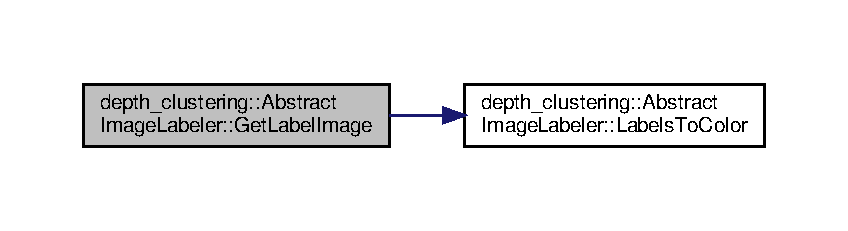
\includegraphics[width=350pt]{classdepth__clustering_1_1AbstractImageLabeler_a7b2f8edf44f3ccb01fb71c296241615e_cgraph}
\end{center}
\end{figure}
\mbox{\Hypertarget{classdepth__clustering_1_1AbstractImageLabeler_abab18e0c1ca40b54922a2f21948b996b}\label{classdepth__clustering_1_1AbstractImageLabeler_abab18e0c1ca40b54922a2f21948b996b}} 
\index{depth\+\_\+clustering\+::\+Abstract\+Image\+Labeler@{depth\+\_\+clustering\+::\+Abstract\+Image\+Labeler}!Labels\+To\+Color@{Labels\+To\+Color}}
\index{Labels\+To\+Color@{Labels\+To\+Color}!depth\+\_\+clustering\+::\+Abstract\+Image\+Labeler@{depth\+\_\+clustering\+::\+Abstract\+Image\+Labeler}}
\subsubsection{\texorpdfstring{Labels\+To\+Color()}{LabelsToColor()}}
{\footnotesize\ttfamily Mat depth\+\_\+clustering\+::\+Abstract\+Image\+Labeler\+::\+Labels\+To\+Color (\begin{DoxyParamCaption}\item[{const cv\+::\+Mat \&}]{label\+\_\+image }\end{DoxyParamCaption})\hspace{0.3cm}{\ttfamily [static]}}



Generates random-\/colored image from image of labels. 


\begin{DoxyParams}[1]{Parameters}
\mbox{\tt in}  & {\em label\+\_\+image} & The label image\\
\hline
\end{DoxyParams}
\begin{DoxyReturn}{Returns}
Random-\/colored image from label image 
\end{DoxyReturn}
Here is the caller graph for this function\+:\nopagebreak
\begin{figure}[H]
\begin{center}
\leavevmode
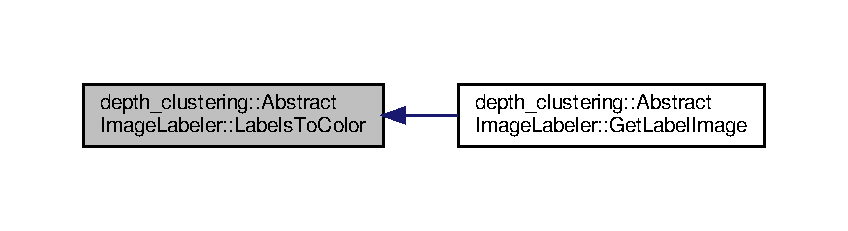
\includegraphics[width=350pt]{classdepth__clustering_1_1AbstractImageLabeler_abab18e0c1ca40b54922a2f21948b996b_icgraph}
\end{center}
\end{figure}


The documentation for this class was generated from the following files\+:\begin{DoxyCompactItemize}
\item 
/home/ashwin/catkin\+\_\+ws/src/depth\+\_\+clustering/src/image\+\_\+labelers/abstract\+\_\+image\+\_\+labeler.\+h\item 
/home/ashwin/catkin\+\_\+ws/src/depth\+\_\+clustering/src/image\+\_\+labelers/abstract\+\_\+image\+\_\+labeler.\+cpp\end{DoxyCompactItemize}

\hypertarget{classdepth__clustering_1_1AbstractSender}{}\section{depth\+\_\+clustering\+:\+:Abstract\+Sender$<$ Obj\+Send\+Type $>$ Class Template Reference}
\label{classdepth__clustering_1_1AbstractSender}\index{depth\+\_\+clustering\+::\+Abstract\+Sender$<$ Obj\+Send\+Type $>$@{depth\+\_\+clustering\+::\+Abstract\+Sender$<$ Obj\+Send\+Type $>$}}


Class for abstract sender.  




{\ttfamily \#include $<$abstract\+\_\+sender.\+h$>$}

\subsection*{Public Member Functions}
\begin{DoxyCompactItemize}
\item 
\mbox{\Hypertarget{classdepth__clustering_1_1AbstractSender_ab04a328c2cc29a97bc3bba2b696c8786}\label{classdepth__clustering_1_1AbstractSender_ab04a328c2cc29a97bc3bba2b696c8786}} 
{\bfseries Abstract\+Sender} (Sender\+Type \hyperlink{classdepth__clustering_1_1AbstractSender_a6120bda97c12587db40f34ed73b45475}{type}=Sender\+Type\+::\+U\+N\+D\+E\+F\+I\+N\+ED)
\item 
const char $\ast$ \hyperlink{classdepth__clustering_1_1AbstractSender_a6120bda97c12587db40f34ed73b45475}{type} () const
\begin{DoxyCompactList}\small\item\em Gets type of sender as string. \end{DoxyCompactList}\item 
void \hyperlink{classdepth__clustering_1_1AbstractSender_aca33c29cca1916fb0a3edd9024a49b51}{Add\+Client} (\hyperlink{classdepth__clustering_1_1AbstractClient}{Abstract\+Client}$<$ Obj\+Send\+Type $>$ $\ast$client)
\begin{DoxyCompactList}\small\item\em Adds a client. \end{DoxyCompactList}\item 
void \hyperlink{classdepth__clustering_1_1AbstractSender_a0c33c98abe8fa71a86f02af95b1c71c1}{Remove\+Client} (int \hyperlink{classdepth__clustering_1_1Identifiable_a50f8b49ce7f7f0d9d02f31f74e0fc9e0}{id})
\begin{DoxyCompactList}\small\item\em Removes a client. \end{DoxyCompactList}\item 
\mbox{\Hypertarget{classdepth__clustering_1_1AbstractSender_ab331127e3e36b15413e1eecf55b5b284}\label{classdepth__clustering_1_1AbstractSender_ab331127e3e36b15413e1eecf55b5b284}} 
void {\bfseries Remove\+Client} (\hyperlink{classdepth__clustering_1_1AbstractClient}{Abstract\+Client}$<$ Obj\+Send\+Type $>$ $\ast$client)
\item 
size\+\_\+t \hyperlink{classdepth__clustering_1_1AbstractSender_a957331eb41f11208bbe6174895c11bf2}{client\+\_\+count} ()
\begin{DoxyCompactList}\small\item\em Get number of clients currently subscribed. \end{DoxyCompactList}\item 
void \hyperlink{classdepth__clustering_1_1AbstractSender_a147752e5ab7ca15da9c8d8e60575390b}{Share\+Data\+With\+All\+Clients} (const Obj\+Send\+Type \&obj, int \hyperlink{classdepth__clustering_1_1Identifiable_a50f8b49ce7f7f0d9d02f31f74e0fc9e0}{id}=-\/1)
\begin{DoxyCompactList}\small\item\em Shares data with everyone who listens to it. \end{DoxyCompactList}\end{DoxyCompactItemize}
\subsection*{Protected Types}
\begin{DoxyCompactItemize}
\item 
\mbox{\Hypertarget{classdepth__clustering_1_1AbstractSender_adc736ec9622d4baf520c8379a23e65ab}\label{classdepth__clustering_1_1AbstractSender_adc736ec9622d4baf520c8379a23e65ab}} 
using {\bfseries Id\+Client\+Mapping} = std\+::map$<$ int, \hyperlink{classdepth__clustering_1_1AbstractClient}{Abstract\+Client}$<$ Obj\+Send\+Type $>$ $\ast$ $>$
\end{DoxyCompactItemize}
\subsection*{Protected Attributes}
\begin{DoxyCompactItemize}
\item 
\mbox{\Hypertarget{classdepth__clustering_1_1AbstractSender_a5ef5e33f2a4a2821b2eb4285fe85f80e}\label{classdepth__clustering_1_1AbstractSender_a5ef5e33f2a4a2821b2eb4285fe85f80e}} 
Id\+Client\+Mapping {\bfseries \+\_\+clients}
\item 
\mbox{\Hypertarget{classdepth__clustering_1_1AbstractSender_a9c837623381f9ec0e26130457286af1a}\label{classdepth__clustering_1_1AbstractSender_a9c837623381f9ec0e26130457286af1a}} 
Sender\+Type {\bfseries \+\_\+type}
\end{DoxyCompactItemize}
\subsection*{Additional Inherited Members}


\subsection{Detailed Description}
\subsubsection*{template$<$class Obj\+Send\+Type$>$\newline
class depth\+\_\+clustering\+::\+Abstract\+Sender$<$ Obj\+Send\+Type $>$}

Class for abstract sender. 


\begin{DoxyTemplParams}{Template Parameters}
{\em Obj\+Send\+Type} & Type of the object to be sent. \\
\hline
\end{DoxyTemplParams}


Inheritance diagram for depth\+\_\+clustering\+:\+:Abstract\+Sender$<$ Obj\+Send\+Type $>$\+:\nopagebreak
\begin{figure}[H]
\begin{center}
\leavevmode
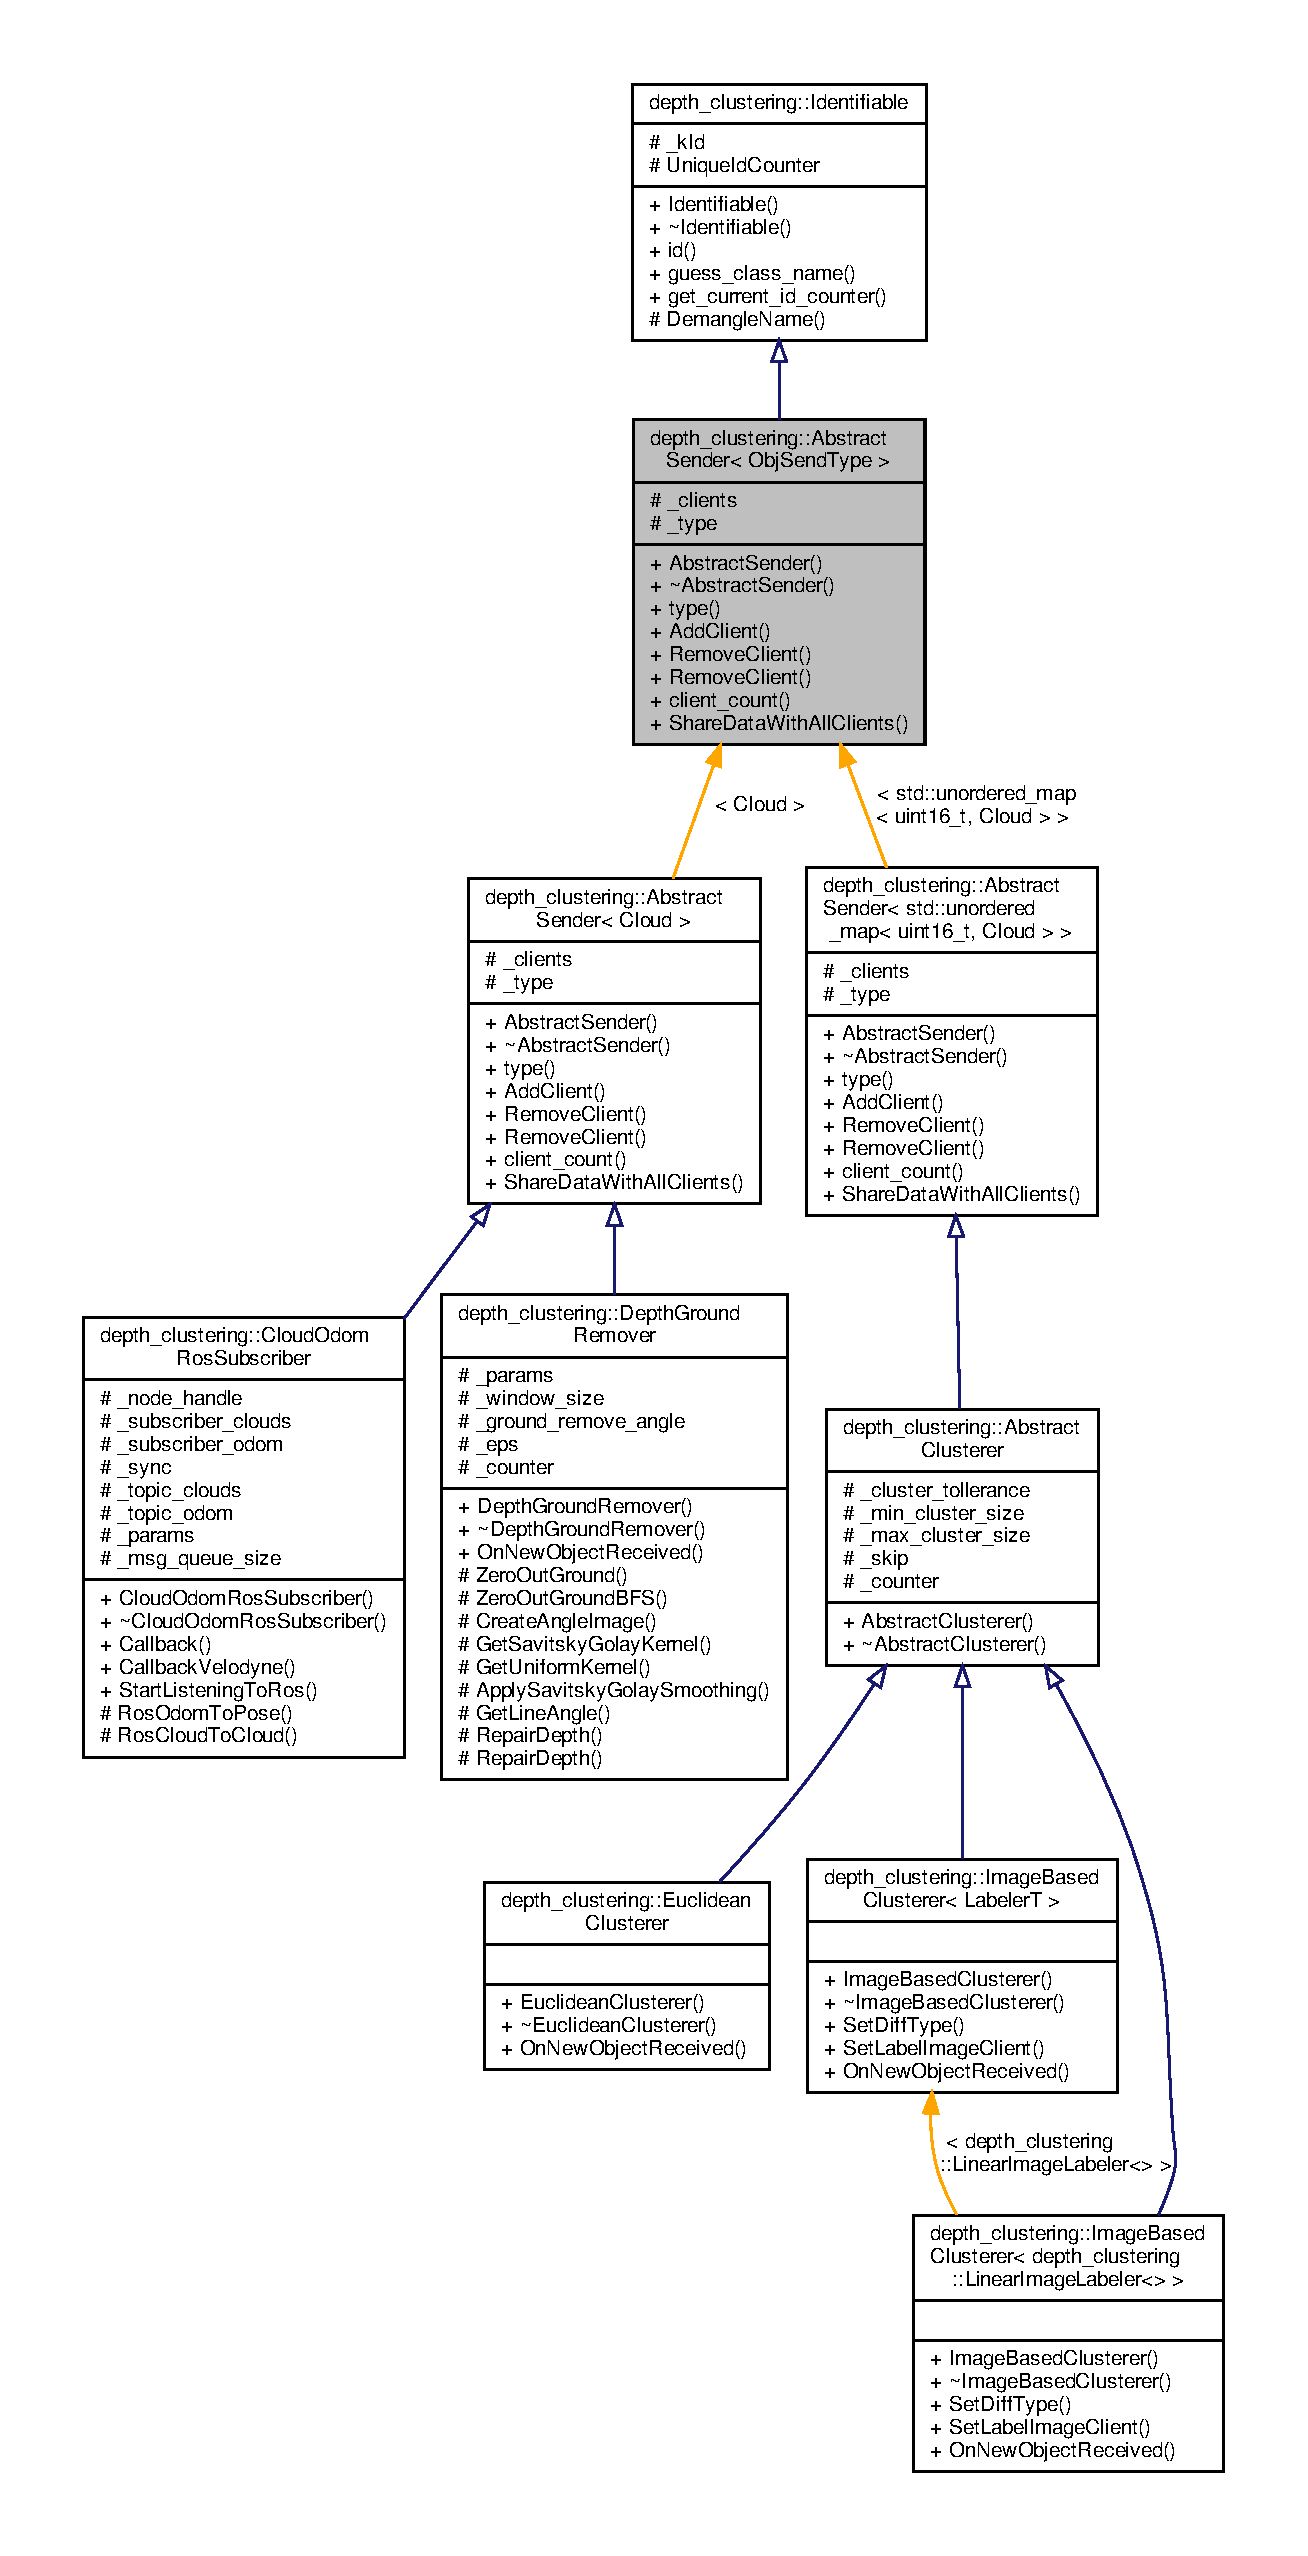
\includegraphics[height=550pt]{classdepth__clustering_1_1AbstractSender__inherit__graph}
\end{center}
\end{figure}


Collaboration diagram for depth\+\_\+clustering\+:\+:Abstract\+Sender$<$ Obj\+Send\+Type $>$\+:\nopagebreak
\begin{figure}[H]
\begin{center}
\leavevmode
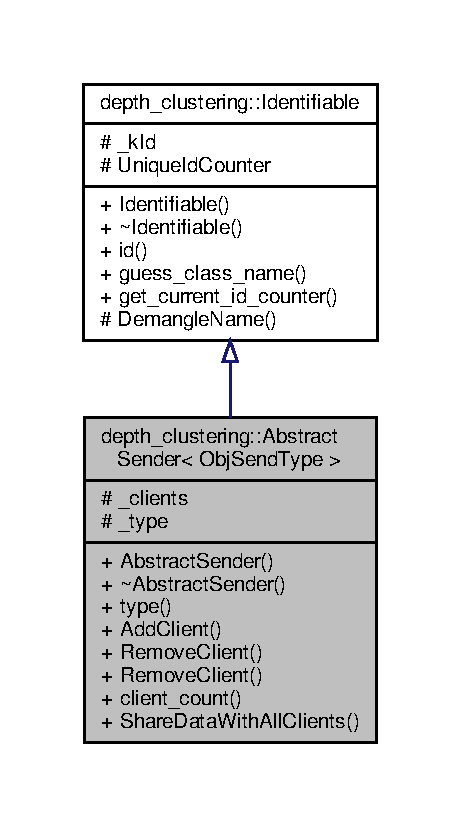
\includegraphics[width=221pt]{classdepth__clustering_1_1AbstractSender__coll__graph}
\end{center}
\end{figure}


\subsection{Member Function Documentation}
\mbox{\Hypertarget{classdepth__clustering_1_1AbstractSender_aca33c29cca1916fb0a3edd9024a49b51}\label{classdepth__clustering_1_1AbstractSender_aca33c29cca1916fb0a3edd9024a49b51}} 
\index{depth\+\_\+clustering\+::\+Abstract\+Sender@{depth\+\_\+clustering\+::\+Abstract\+Sender}!Add\+Client@{Add\+Client}}
\index{Add\+Client@{Add\+Client}!depth\+\_\+clustering\+::\+Abstract\+Sender@{depth\+\_\+clustering\+::\+Abstract\+Sender}}
\subsubsection{\texorpdfstring{Add\+Client()}{AddClient()}}
{\footnotesize\ttfamily template$<$class Obj\+Send\+Type$>$ \\
void \hyperlink{classdepth__clustering_1_1AbstractSender}{depth\+\_\+clustering\+::\+Abstract\+Sender}$<$ Obj\+Send\+Type $>$\+::Add\+Client (\begin{DoxyParamCaption}\item[{\hyperlink{classdepth__clustering_1_1AbstractClient}{Abstract\+Client}$<$ Obj\+Send\+Type $>$ $\ast$}]{client }\end{DoxyParamCaption})\hspace{0.3cm}{\ttfamily [inline]}}



Adds a client. 


\begin{DoxyParams}{Parameters}
{\em client} & The client to receive the processed data \\
\hline
\end{DoxyParams}
\mbox{\Hypertarget{classdepth__clustering_1_1AbstractSender_a957331eb41f11208bbe6174895c11bf2}\label{classdepth__clustering_1_1AbstractSender_a957331eb41f11208bbe6174895c11bf2}} 
\index{depth\+\_\+clustering\+::\+Abstract\+Sender@{depth\+\_\+clustering\+::\+Abstract\+Sender}!client\+\_\+count@{client\+\_\+count}}
\index{client\+\_\+count@{client\+\_\+count}!depth\+\_\+clustering\+::\+Abstract\+Sender@{depth\+\_\+clustering\+::\+Abstract\+Sender}}
\subsubsection{\texorpdfstring{client\+\_\+count()}{client\_count()}}
{\footnotesize\ttfamily template$<$class Obj\+Send\+Type$>$ \\
size\+\_\+t \hyperlink{classdepth__clustering_1_1AbstractSender}{depth\+\_\+clustering\+::\+Abstract\+Sender}$<$ Obj\+Send\+Type $>$\+::client\+\_\+count (\begin{DoxyParamCaption}{ }\end{DoxyParamCaption})\hspace{0.3cm}{\ttfamily [inline]}}



Get number of clients currently subscribed. 

\begin{DoxyReturn}{Returns}
Current number of Clients 
\end{DoxyReturn}
\mbox{\Hypertarget{classdepth__clustering_1_1AbstractSender_a0c33c98abe8fa71a86f02af95b1c71c1}\label{classdepth__clustering_1_1AbstractSender_a0c33c98abe8fa71a86f02af95b1c71c1}} 
\index{depth\+\_\+clustering\+::\+Abstract\+Sender@{depth\+\_\+clustering\+::\+Abstract\+Sender}!Remove\+Client@{Remove\+Client}}
\index{Remove\+Client@{Remove\+Client}!depth\+\_\+clustering\+::\+Abstract\+Sender@{depth\+\_\+clustering\+::\+Abstract\+Sender}}
\subsubsection{\texorpdfstring{Remove\+Client()}{RemoveClient()}}
{\footnotesize\ttfamily template$<$class Obj\+Send\+Type$>$ \\
void \hyperlink{classdepth__clustering_1_1AbstractSender}{depth\+\_\+clustering\+::\+Abstract\+Sender}$<$ Obj\+Send\+Type $>$\+::Remove\+Client (\begin{DoxyParamCaption}\item[{int}]{id }\end{DoxyParamCaption})\hspace{0.3cm}{\ttfamily [inline]}}



Removes a client. 


\begin{DoxyParams}[1]{Parameters}
\mbox{\tt in}  & {\em id} & The identifier of the client to remove \\
\hline
\end{DoxyParams}
\mbox{\Hypertarget{classdepth__clustering_1_1AbstractSender_a147752e5ab7ca15da9c8d8e60575390b}\label{classdepth__clustering_1_1AbstractSender_a147752e5ab7ca15da9c8d8e60575390b}} 
\index{depth\+\_\+clustering\+::\+Abstract\+Sender@{depth\+\_\+clustering\+::\+Abstract\+Sender}!Share\+Data\+With\+All\+Clients@{Share\+Data\+With\+All\+Clients}}
\index{Share\+Data\+With\+All\+Clients@{Share\+Data\+With\+All\+Clients}!depth\+\_\+clustering\+::\+Abstract\+Sender@{depth\+\_\+clustering\+::\+Abstract\+Sender}}
\subsubsection{\texorpdfstring{Share\+Data\+With\+All\+Clients()}{ShareDataWithAllClients()}}
{\footnotesize\ttfamily template$<$class Obj\+Send\+Type$>$ \\
void \hyperlink{classdepth__clustering_1_1AbstractSender}{depth\+\_\+clustering\+::\+Abstract\+Sender}$<$ Obj\+Send\+Type $>$\+::Share\+Data\+With\+All\+Clients (\begin{DoxyParamCaption}\item[{const Obj\+Send\+Type \&}]{obj,  }\item[{int}]{id = {\ttfamily -\/1} }\end{DoxyParamCaption})\hspace{0.3cm}{\ttfamily [inline]}}



Shares data with everyone who listens to it. 


\begin{DoxyParams}[1]{Parameters}
\mbox{\tt in}  & {\em obj} & Object to share \\
\hline
\mbox{\tt in}  & {\em id} & Id, by default this-\/$>$\hyperlink{classdepth__clustering_1_1Identifiable_a50f8b49ce7f7f0d9d02f31f74e0fc9e0}{id()} \\
\hline
\end{DoxyParams}
\mbox{\Hypertarget{classdepth__clustering_1_1AbstractSender_a6120bda97c12587db40f34ed73b45475}\label{classdepth__clustering_1_1AbstractSender_a6120bda97c12587db40f34ed73b45475}} 
\index{depth\+\_\+clustering\+::\+Abstract\+Sender@{depth\+\_\+clustering\+::\+Abstract\+Sender}!type@{type}}
\index{type@{type}!depth\+\_\+clustering\+::\+Abstract\+Sender@{depth\+\_\+clustering\+::\+Abstract\+Sender}}
\subsubsection{\texorpdfstring{type()}{type()}}
{\footnotesize\ttfamily template$<$class Obj\+Send\+Type$>$ \\
const char$\ast$ \hyperlink{classdepth__clustering_1_1AbstractSender}{depth\+\_\+clustering\+::\+Abstract\+Sender}$<$ Obj\+Send\+Type $>$\+::type (\begin{DoxyParamCaption}{ }\end{DoxyParamCaption}) const\hspace{0.3cm}{\ttfamily [inline]}}



Gets type of sender as string. 

\begin{DoxyReturn}{Returns}
Type as string 
\end{DoxyReturn}


The documentation for this class was generated from the following file\+:\begin{DoxyCompactItemize}
\item 
/home/ashwin/catkin\+\_\+ws/src/depth\+\_\+clustering/src/communication/abstract\+\_\+sender.\+h\end{DoxyCompactItemize}

\hypertarget{classdepth__clustering_1_1AngleDiff}{}\section{depth\+\_\+clustering\+:\+:Angle\+Diff Class Reference}
\label{classdepth__clustering_1_1AngleDiff}\index{depth\+\_\+clustering\+::\+Angle\+Diff@{depth\+\_\+clustering\+::\+Angle\+Diff}}


Class for angle difference.  




{\ttfamily \#include $<$angle\+\_\+diff.\+h$>$}

\subsection*{Public Member Functions}
\begin{DoxyCompactItemize}
\item 
\hyperlink{classdepth__clustering_1_1AngleDiff_a40371150bff3a10dd8ce40788b9bd160}{Angle\+Diff} (const cv\+::\+Mat $\ast$source\+\_\+image, const \hyperlink{classdepth__clustering_1_1ProjectionParams}{Projection\+Params} $\ast$params)
\begin{DoxyCompactList}\small\item\em Precompute the angles to avoid losing time on that. \end{DoxyCompactList}\item 
float \hyperlink{classdepth__clustering_1_1AngleDiff_ac9bd0ec61ff0b213fd19235dc171c1c2}{Diff\+At} (const \hyperlink{structdepth__clustering_1_1PixelCoord}{Pixel\+Coord} \&from, const \hyperlink{structdepth__clustering_1_1PixelCoord}{Pixel\+Coord} \&to) const override
\begin{DoxyCompactList}\small\item\em Compute angle-\/based difference. See paper for details. \end{DoxyCompactList}\item 
\mbox{\Hypertarget{classdepth__clustering_1_1AngleDiff_ac65e8f42b1f2ac82db14ebe188c004a2}\label{classdepth__clustering_1_1AngleDiff_ac65e8f42b1f2ac82db14ebe188c004a2}} 
bool \hyperlink{classdepth__clustering_1_1AngleDiff_ac65e8f42b1f2ac82db14ebe188c004a2}{Satisfies\+Threshold} (float angle, float threshold) const override
\begin{DoxyCompactList}\small\item\em Threshold is satisfied if angle is B\+I\+G\+G\+ER than threshold. \end{DoxyCompactList}\item 
cv\+::\+Mat \hyperlink{classdepth__clustering_1_1AngleDiff_a462e4aadd35ca06e9b061d08c9787074}{Visualize} () const override
\begin{DoxyCompactList}\small\item\em Visualize $\beta$ angles as a {\ttfamily cv\+::\+Mat} color image. \end{DoxyCompactList}\end{DoxyCompactItemize}
\subsection*{Additional Inherited Members}


\subsection{Detailed Description}
Class for angle difference. 

Inheritance diagram for depth\+\_\+clustering\+:\+:Angle\+Diff\+:\nopagebreak
\begin{figure}[H]
\begin{center}
\leavevmode
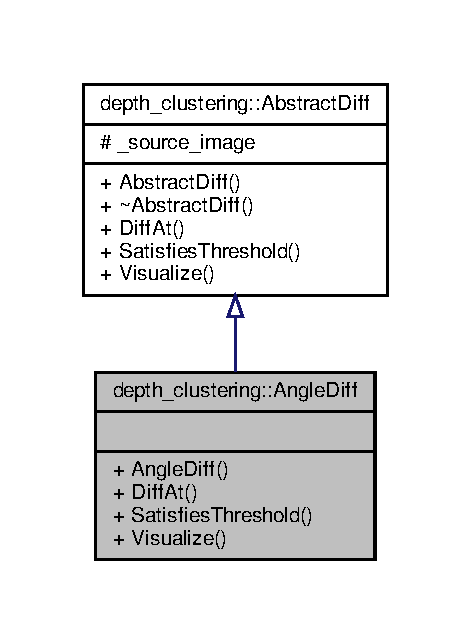
\includegraphics[width=226pt]{classdepth__clustering_1_1AngleDiff__inherit__graph}
\end{center}
\end{figure}


Collaboration diagram for depth\+\_\+clustering\+:\+:Angle\+Diff\+:\nopagebreak
\begin{figure}[H]
\begin{center}
\leavevmode
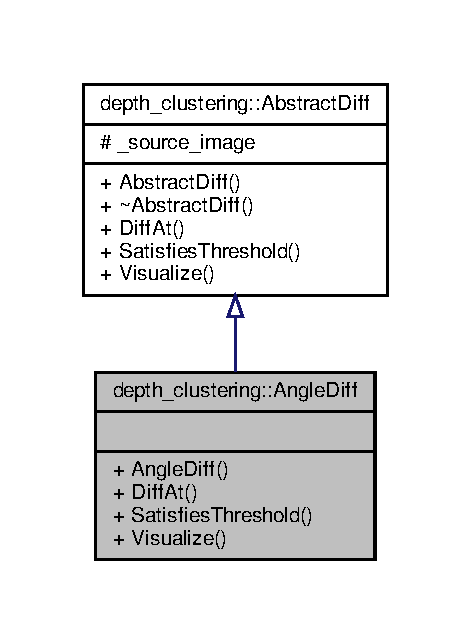
\includegraphics[width=226pt]{classdepth__clustering_1_1AngleDiff__coll__graph}
\end{center}
\end{figure}


\subsection{Constructor \& Destructor Documentation}
\mbox{\Hypertarget{classdepth__clustering_1_1AngleDiff_a40371150bff3a10dd8ce40788b9bd160}\label{classdepth__clustering_1_1AngleDiff_a40371150bff3a10dd8ce40788b9bd160}} 
\index{depth\+\_\+clustering\+::\+Angle\+Diff@{depth\+\_\+clustering\+::\+Angle\+Diff}!Angle\+Diff@{Angle\+Diff}}
\index{Angle\+Diff@{Angle\+Diff}!depth\+\_\+clustering\+::\+Angle\+Diff@{depth\+\_\+clustering\+::\+Angle\+Diff}}
\subsubsection{\texorpdfstring{Angle\+Diff()}{AngleDiff()}}
{\footnotesize\ttfamily depth\+\_\+clustering\+::\+Angle\+Diff\+::\+Angle\+Diff (\begin{DoxyParamCaption}\item[{const cv\+::\+Mat $\ast$}]{source\+\_\+image,  }\item[{const \hyperlink{classdepth__clustering_1_1ProjectionParams}{Projection\+Params} $\ast$}]{params }\end{DoxyParamCaption})}



Precompute the angles to avoid losing time on that. 


\begin{DoxyParams}[1]{Parameters}
\mbox{\tt in}  & {\em source\+\_\+image} & The source image \\
\hline
\mbox{\tt in}  & {\em params} & The projection parameters \\
\hline
\end{DoxyParams}


\subsection{Member Function Documentation}
\mbox{\Hypertarget{classdepth__clustering_1_1AngleDiff_ac9bd0ec61ff0b213fd19235dc171c1c2}\label{classdepth__clustering_1_1AngleDiff_ac9bd0ec61ff0b213fd19235dc171c1c2}} 
\index{depth\+\_\+clustering\+::\+Angle\+Diff@{depth\+\_\+clustering\+::\+Angle\+Diff}!Diff\+At@{Diff\+At}}
\index{Diff\+At@{Diff\+At}!depth\+\_\+clustering\+::\+Angle\+Diff@{depth\+\_\+clustering\+::\+Angle\+Diff}}
\subsubsection{\texorpdfstring{Diff\+At()}{DiffAt()}}
{\footnotesize\ttfamily float depth\+\_\+clustering\+::\+Angle\+Diff\+::\+Diff\+At (\begin{DoxyParamCaption}\item[{const \hyperlink{structdepth__clustering_1_1PixelCoord}{Pixel\+Coord} \&}]{from,  }\item[{const \hyperlink{structdepth__clustering_1_1PixelCoord}{Pixel\+Coord} \&}]{to }\end{DoxyParamCaption}) const\hspace{0.3cm}{\ttfamily [override]}, {\ttfamily [virtual]}}



Compute angle-\/based difference. See paper for details. 


\begin{DoxyParams}[1]{Parameters}
\mbox{\tt in}  & {\em from} & Pixel from which to compute difference \\
\hline
\mbox{\tt in}  & {\em to} & Pixel to which to compute difference\\
\hline
\end{DoxyParams}
\begin{DoxyReturn}{Returns}
Angle difference between the values 
\end{DoxyReturn}


Implements \hyperlink{classdepth__clustering_1_1AbstractDiff_a06ba188d8d83d0e4bad66c833656c26d}{depth\+\_\+clustering\+::\+Abstract\+Diff}.

Here is the call graph for this function\+:\nopagebreak
\begin{figure}[H]
\begin{center}
\leavevmode
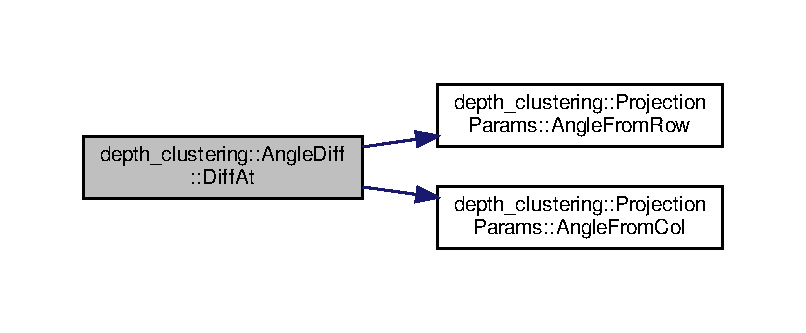
\includegraphics[width=350pt]{classdepth__clustering_1_1AngleDiff_ac9bd0ec61ff0b213fd19235dc171c1c2_cgraph}
\end{center}
\end{figure}
\mbox{\Hypertarget{classdepth__clustering_1_1AngleDiff_a462e4aadd35ca06e9b061d08c9787074}\label{classdepth__clustering_1_1AngleDiff_a462e4aadd35ca06e9b061d08c9787074}} 
\index{depth\+\_\+clustering\+::\+Angle\+Diff@{depth\+\_\+clustering\+::\+Angle\+Diff}!Visualize@{Visualize}}
\index{Visualize@{Visualize}!depth\+\_\+clustering\+::\+Angle\+Diff@{depth\+\_\+clustering\+::\+Angle\+Diff}}
\subsubsection{\texorpdfstring{Visualize()}{Visualize()}}
{\footnotesize\ttfamily cv\+::\+Mat depth\+\_\+clustering\+::\+Angle\+Diff\+::\+Visualize (\begin{DoxyParamCaption}{ }\end{DoxyParamCaption}) const\hspace{0.3cm}{\ttfamily [inline]}, {\ttfamily [override]}, {\ttfamily [virtual]}}



Visualize $\beta$ angles as a {\ttfamily cv\+::\+Mat} color image. 

\begin{DoxyReturn}{Returns}
{\ttfamily cv\+::\+Mat} color image with red channel showing $\beta$ angles in row direction and green channel in col direction. 
\end{DoxyReturn}


Reimplemented from \hyperlink{classdepth__clustering_1_1AbstractDiff_a45314bf711f35e53590af28bdfc45313}{depth\+\_\+clustering\+::\+Abstract\+Diff}.

Here is the caller graph for this function\+:\nopagebreak
\begin{figure}[H]
\begin{center}
\leavevmode
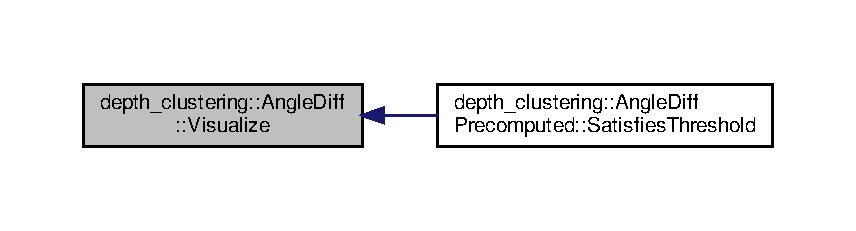
\includegraphics[width=350pt]{classdepth__clustering_1_1AngleDiff_a462e4aadd35ca06e9b061d08c9787074_icgraph}
\end{center}
\end{figure}


The documentation for this class was generated from the following files\+:\begin{DoxyCompactItemize}
\item 
/home/ashwin/catkin\+\_\+ws/src/depth\+\_\+clustering/src/image\+\_\+labelers/diff\+\_\+helpers/angle\+\_\+diff.\+h\item 
/home/ashwin/catkin\+\_\+ws/src/depth\+\_\+clustering/src/image\+\_\+labelers/diff\+\_\+helpers/angle\+\_\+diff.\+cpp\end{DoxyCompactItemize}

\hypertarget{classdepth__clustering_1_1AngleDiffPrecomputed}{}\section{depth\+\_\+clustering\+:\+:Angle\+Diff\+Precomputed Class Reference}
\label{classdepth__clustering_1_1AngleDiffPrecomputed}\index{depth\+\_\+clustering\+::\+Angle\+Diff\+Precomputed@{depth\+\_\+clustering\+::\+Angle\+Diff\+Precomputed}}


Class for angle difference.  




{\ttfamily \#include $<$angle\+\_\+diff.\+h$>$}

\subsection*{Public Member Functions}
\begin{DoxyCompactItemize}
\item 
\hyperlink{classdepth__clustering_1_1AngleDiffPrecomputed_a0cd5a0071d191d6a4f3594a789777ff3}{Angle\+Diff\+Precomputed} (const cv\+::\+Mat $\ast$source\+\_\+image, const \hyperlink{classdepth__clustering_1_1ProjectionParams}{Projection\+Params} $\ast$params)
\begin{DoxyCompactList}\small\item\em Precompute the angles to avoid losing time on that. \end{DoxyCompactList}\item 
float \hyperlink{classdepth__clustering_1_1AngleDiffPrecomputed_ae15bb5fc9488ae2b26c77665931b8626}{Diff\+At} (const \hyperlink{structdepth__clustering_1_1PixelCoord}{Pixel\+Coord} \&from, const \hyperlink{structdepth__clustering_1_1PixelCoord}{Pixel\+Coord} \&to) const override
\begin{DoxyCompactList}\small\item\em Compute angle-\/based difference. See paper for details. Only one of the following situations is possible\+: \end{DoxyCompactList}\item 
\mbox{\Hypertarget{classdepth__clustering_1_1AngleDiffPrecomputed_a28a32c0cb0405163fe237909fe5f6c0c}\label{classdepth__clustering_1_1AngleDiffPrecomputed_a28a32c0cb0405163fe237909fe5f6c0c}} 
bool \hyperlink{classdepth__clustering_1_1AngleDiffPrecomputed_a28a32c0cb0405163fe237909fe5f6c0c}{Satisfies\+Threshold} (float angle, float threshold) const override
\begin{DoxyCompactList}\small\item\em Threshold is satisfied if angle is B\+I\+G\+G\+ER than threshold. \end{DoxyCompactList}\item 
cv\+::\+Mat \hyperlink{classdepth__clustering_1_1AngleDiffPrecomputed_a2fd85404d06843af0ee5c713017f6641}{Visualize} () const
\begin{DoxyCompactList}\small\item\em Visualize $\beta$ angles as a {\ttfamily cv\+::\+Mat} color image. \end{DoxyCompactList}\end{DoxyCompactItemize}
\subsection*{Protected Member Functions}
\begin{DoxyCompactItemize}
\item 
\mbox{\Hypertarget{classdepth__clustering_1_1AngleDiffPrecomputed_a8f333b5196e9dcaa7923f82d362c7281}\label{classdepth__clustering_1_1AngleDiffPrecomputed_a8f333b5196e9dcaa7923f82d362c7281}} 
void \hyperlink{classdepth__clustering_1_1AngleDiffPrecomputed_a8f333b5196e9dcaa7923f82d362c7281}{Pre\+Compute\+Alpha\+Vecs} ()
\begin{DoxyCompactList}\small\item\em Pre-\/compute values for angles for all cols and rows. \end{DoxyCompactList}\item 
void \hyperlink{classdepth__clustering_1_1AngleDiffPrecomputed_aeb86ee61c6e8fc1b5b554368b1f5fa27}{Pre\+Compute\+Beta\+Angles} ()
\begin{DoxyCompactList}\small\item\em Precompute all $\beta$ angles for the image. It generates two matrices for row-\/wise and col-\/wise angles. See picture for illustration. The squares store values of angles between pixels with computation direction shown by arrows. Note that the columns matrix wraps around, i.\+e. the last element stores the difference in angles between the last pixel of the original image and the first one. \end{DoxyCompactList}\item 
float \hyperlink{classdepth__clustering_1_1AngleDiffPrecomputed_aa67b440539cd571a990af5131a5b1ec0}{Get\+Beta} (float alpha, float current\+\_\+depth, float neighbor\+\_\+depth) const
\begin{DoxyCompactList}\small\item\em Compute the angle $\beta$ of incline of the line spawned by two given beams. \end{DoxyCompactList}\end{DoxyCompactItemize}
\subsection*{Protected Attributes}
\begin{DoxyCompactItemize}
\item 
\mbox{\Hypertarget{classdepth__clustering_1_1AngleDiffPrecomputed_ac37e01df194d9063b7e7bd1f7b7aa6a4}\label{classdepth__clustering_1_1AngleDiffPrecomputed_ac37e01df194d9063b7e7bd1f7b7aa6a4}} 
const \hyperlink{classdepth__clustering_1_1ProjectionParams}{Projection\+Params} $\ast$ {\bfseries \+\_\+params} = nullptr
\item 
\mbox{\Hypertarget{classdepth__clustering_1_1AngleDiffPrecomputed_a2ba86b3ed5f12c2a7e2e8beef81bd88d}\label{classdepth__clustering_1_1AngleDiffPrecomputed_a2ba86b3ed5f12c2a7e2e8beef81bd88d}} 
std\+::vector$<$ float $>$ {\bfseries \+\_\+row\+\_\+alphas}
\item 
\mbox{\Hypertarget{classdepth__clustering_1_1AngleDiffPrecomputed_a90f6e3fd2f4b585c2cd03809f3818ee9}\label{classdepth__clustering_1_1AngleDiffPrecomputed_a90f6e3fd2f4b585c2cd03809f3818ee9}} 
std\+::vector$<$ float $>$ {\bfseries \+\_\+col\+\_\+alphas}
\item 
\mbox{\Hypertarget{classdepth__clustering_1_1AngleDiffPrecomputed_a2df8751352e4621cb69743801e151b75}\label{classdepth__clustering_1_1AngleDiffPrecomputed_a2df8751352e4621cb69743801e151b75}} 
cv\+::\+Mat {\bfseries \+\_\+beta\+\_\+rows}
\item 
\mbox{\Hypertarget{classdepth__clustering_1_1AngleDiffPrecomputed_ae7faa81ea82d0ff9f75f8a1e63659ced}\label{classdepth__clustering_1_1AngleDiffPrecomputed_ae7faa81ea82d0ff9f75f8a1e63659ced}} 
cv\+::\+Mat {\bfseries \+\_\+beta\+\_\+cols}
\end{DoxyCompactItemize}


\subsection{Detailed Description}
Class for angle difference. 

Inheritance diagram for depth\+\_\+clustering\+:\+:Angle\+Diff\+Precomputed\+:\nopagebreak
\begin{figure}[H]
\begin{center}
\leavevmode
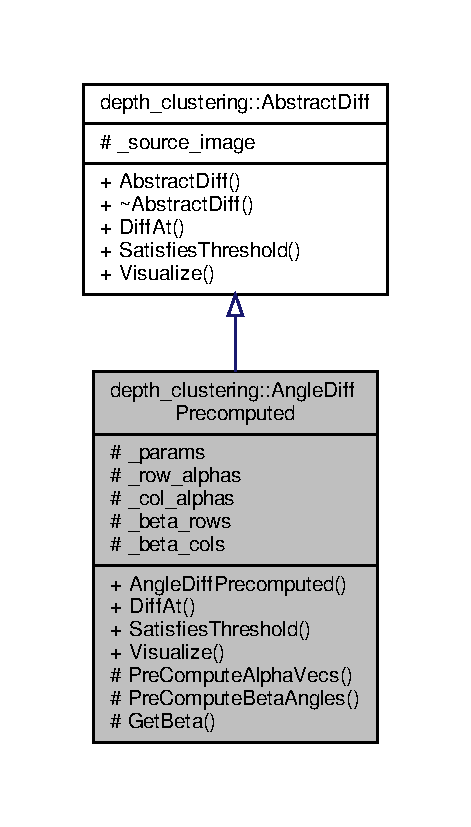
\includegraphics[width=226pt]{classdepth__clustering_1_1AngleDiffPrecomputed__inherit__graph}
\end{center}
\end{figure}


Collaboration diagram for depth\+\_\+clustering\+:\+:Angle\+Diff\+Precomputed\+:\nopagebreak
\begin{figure}[H]
\begin{center}
\leavevmode
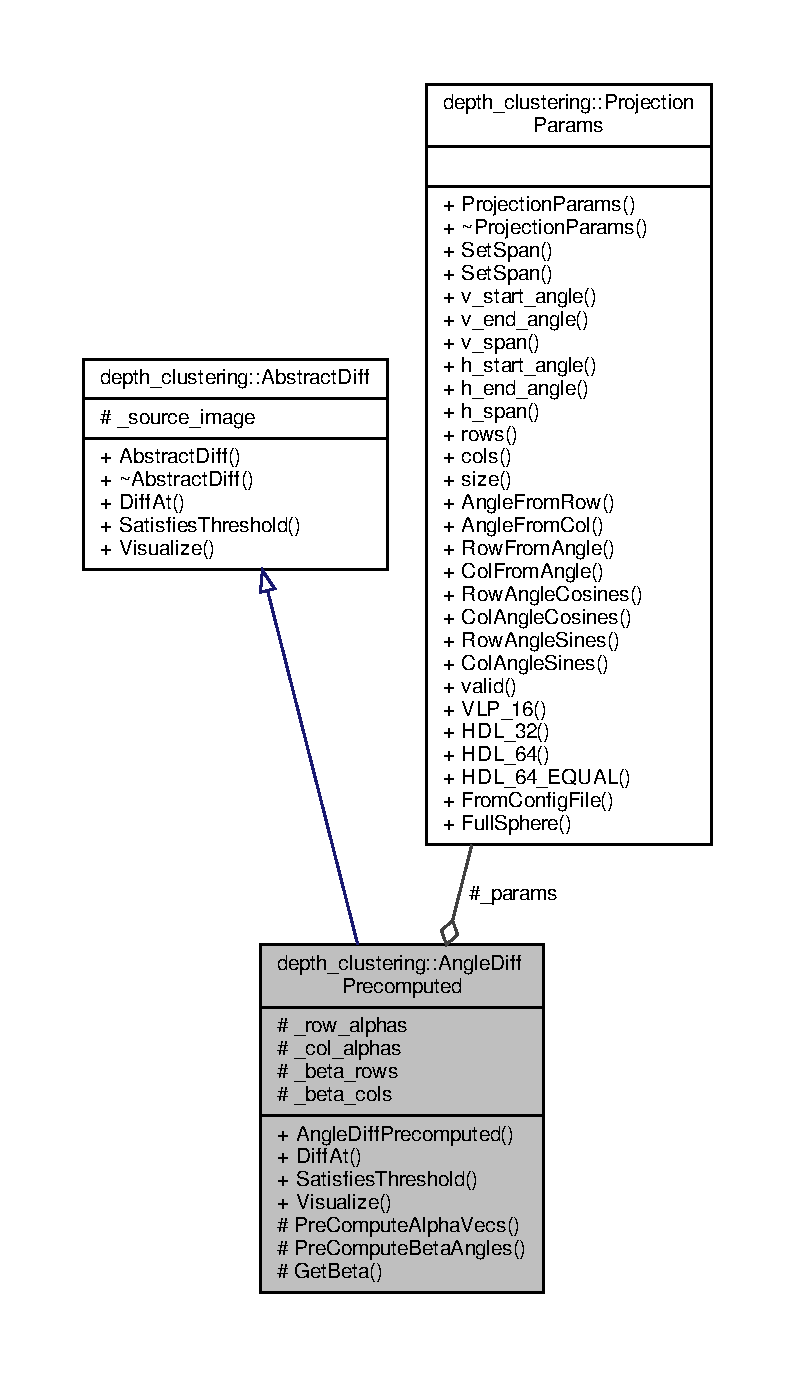
\includegraphics[height=550pt]{classdepth__clustering_1_1AngleDiffPrecomputed__coll__graph}
\end{center}
\end{figure}


\subsection{Constructor \& Destructor Documentation}
\mbox{\Hypertarget{classdepth__clustering_1_1AngleDiffPrecomputed_a0cd5a0071d191d6a4f3594a789777ff3}\label{classdepth__clustering_1_1AngleDiffPrecomputed_a0cd5a0071d191d6a4f3594a789777ff3}} 
\index{depth\+\_\+clustering\+::\+Angle\+Diff\+Precomputed@{depth\+\_\+clustering\+::\+Angle\+Diff\+Precomputed}!Angle\+Diff\+Precomputed@{Angle\+Diff\+Precomputed}}
\index{Angle\+Diff\+Precomputed@{Angle\+Diff\+Precomputed}!depth\+\_\+clustering\+::\+Angle\+Diff\+Precomputed@{depth\+\_\+clustering\+::\+Angle\+Diff\+Precomputed}}
\subsubsection{\texorpdfstring{Angle\+Diff\+Precomputed()}{AngleDiffPrecomputed()}}
{\footnotesize\ttfamily depth\+\_\+clustering\+::\+Angle\+Diff\+Precomputed\+::\+Angle\+Diff\+Precomputed (\begin{DoxyParamCaption}\item[{const cv\+::\+Mat $\ast$}]{source\+\_\+image,  }\item[{const \hyperlink{classdepth__clustering_1_1ProjectionParams}{Projection\+Params} $\ast$}]{params }\end{DoxyParamCaption})}



Precompute the angles to avoid losing time on that. 


\begin{DoxyParams}[1]{Parameters}
\mbox{\tt in}  & {\em source\+\_\+image} & The source image \\
\hline
\mbox{\tt in}  & {\em params} & The projection parameters \\
\hline
\end{DoxyParams}
Here is the call graph for this function\+:\nopagebreak
\begin{figure}[H]
\begin{center}
\leavevmode
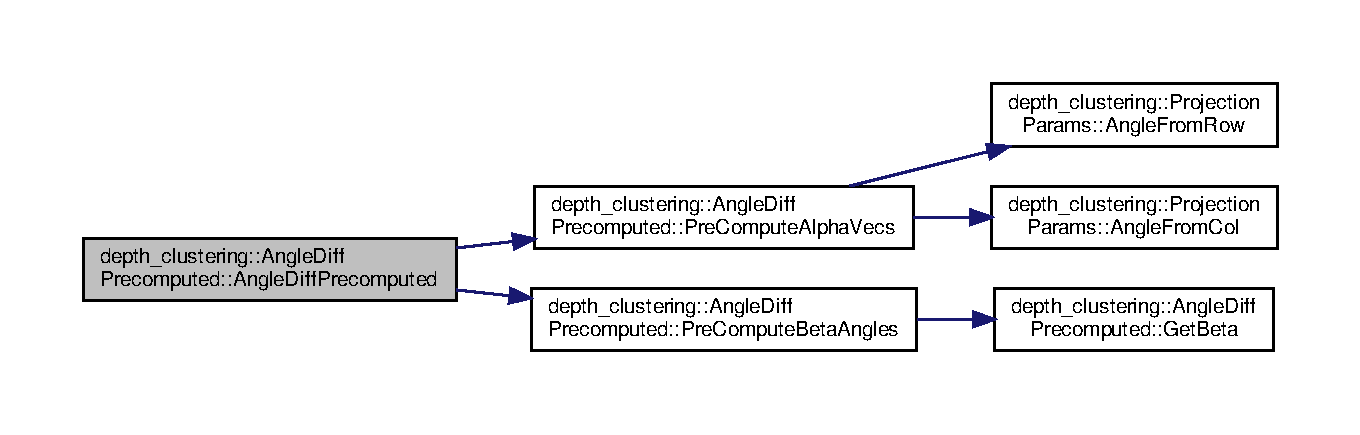
\includegraphics[width=350pt]{classdepth__clustering_1_1AngleDiffPrecomputed_a0cd5a0071d191d6a4f3594a789777ff3_cgraph}
\end{center}
\end{figure}


\subsection{Member Function Documentation}
\mbox{\Hypertarget{classdepth__clustering_1_1AngleDiffPrecomputed_ae15bb5fc9488ae2b26c77665931b8626}\label{classdepth__clustering_1_1AngleDiffPrecomputed_ae15bb5fc9488ae2b26c77665931b8626}} 
\index{depth\+\_\+clustering\+::\+Angle\+Diff\+Precomputed@{depth\+\_\+clustering\+::\+Angle\+Diff\+Precomputed}!Diff\+At@{Diff\+At}}
\index{Diff\+At@{Diff\+At}!depth\+\_\+clustering\+::\+Angle\+Diff\+Precomputed@{depth\+\_\+clustering\+::\+Angle\+Diff\+Precomputed}}
\subsubsection{\texorpdfstring{Diff\+At()}{DiffAt()}}
{\footnotesize\ttfamily float depth\+\_\+clustering\+::\+Angle\+Diff\+Precomputed\+::\+Diff\+At (\begin{DoxyParamCaption}\item[{const \hyperlink{structdepth__clustering_1_1PixelCoord}{Pixel\+Coord} \&}]{from,  }\item[{const \hyperlink{structdepth__clustering_1_1PixelCoord}{Pixel\+Coord} \&}]{to }\end{DoxyParamCaption}) const\hspace{0.3cm}{\ttfamily [override]}, {\ttfamily [virtual]}}



Compute angle-\/based difference. See paper for details. Only one of the following situations is possible\+: 


\begin{DoxyItemize}
\item from.\+row $>$ to.\+row
\item from.\+row $<$ to.\+row
\item from.\+col $>$ to.\+col
\item from.\+col $<$ to.\+col
\end{DoxyItemize}


\begin{DoxyParams}[1]{Parameters}
\mbox{\tt in}  & {\em from} & Pixel from which to compute difference \\
\hline
\mbox{\tt in}  & {\em to} & Pixel to which to compute difference\\
\hline
\end{DoxyParams}
\begin{DoxyReturn}{Returns}
Angle difference between the values 
\end{DoxyReturn}
If one of rows is biggest possible -\/ use it. Otherwise use {\ttfamily std\+::min(from.\+row, to.\+row)}.

If one of cols is biggest possible -\/ use it. Otherwise use {\ttfamily std\+::min(from.\+col, to.\+col)}. 

Implements \hyperlink{classdepth__clustering_1_1AbstractDiff_a06ba188d8d83d0e4bad66c833656c26d}{depth\+\_\+clustering\+::\+Abstract\+Diff}.

\mbox{\Hypertarget{classdepth__clustering_1_1AngleDiffPrecomputed_aa67b440539cd571a990af5131a5b1ec0}\label{classdepth__clustering_1_1AngleDiffPrecomputed_aa67b440539cd571a990af5131a5b1ec0}} 
\index{depth\+\_\+clustering\+::\+Angle\+Diff\+Precomputed@{depth\+\_\+clustering\+::\+Angle\+Diff\+Precomputed}!Get\+Beta@{Get\+Beta}}
\index{Get\+Beta@{Get\+Beta}!depth\+\_\+clustering\+::\+Angle\+Diff\+Precomputed@{depth\+\_\+clustering\+::\+Angle\+Diff\+Precomputed}}
\subsubsection{\texorpdfstring{Get\+Beta()}{GetBeta()}}
{\footnotesize\ttfamily float depth\+\_\+clustering\+::\+Angle\+Diff\+Precomputed\+::\+Get\+Beta (\begin{DoxyParamCaption}\item[{float}]{alpha,  }\item[{float}]{current\+\_\+depth,  }\item[{float}]{neighbor\+\_\+depth }\end{DoxyParamCaption}) const\hspace{0.3cm}{\ttfamily [protected]}}



Compute the angle $\beta$ of incline of the line spawned by two given beams. 


\begin{DoxyParams}[1]{Parameters}
\mbox{\tt in}  & {\em alpha} & The angle $\alpha$ between the beams. \\
\hline
\mbox{\tt in}  & {\em current\+\_\+depth} & The reading of the first beam in meters. \\
\hline
\mbox{\tt in}  & {\em neighbor\+\_\+depth} & The reading of the second beam in meters.\\
\hline
\end{DoxyParams}
\begin{DoxyReturn}{Returns}
The angle of incidence of the line spawned by endpoints of two given beams. 
\end{DoxyReturn}
Here is the caller graph for this function\+:\nopagebreak
\begin{figure}[H]
\begin{center}
\leavevmode
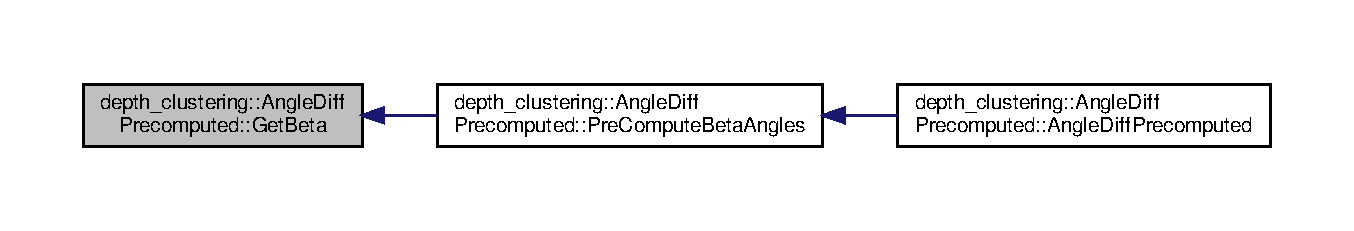
\includegraphics[width=350pt]{classdepth__clustering_1_1AngleDiffPrecomputed_aa67b440539cd571a990af5131a5b1ec0_icgraph}
\end{center}
\end{figure}
\mbox{\Hypertarget{classdepth__clustering_1_1AngleDiffPrecomputed_aeb86ee61c6e8fc1b5b554368b1f5fa27}\label{classdepth__clustering_1_1AngleDiffPrecomputed_aeb86ee61c6e8fc1b5b554368b1f5fa27}} 
\index{depth\+\_\+clustering\+::\+Angle\+Diff\+Precomputed@{depth\+\_\+clustering\+::\+Angle\+Diff\+Precomputed}!Pre\+Compute\+Beta\+Angles@{Pre\+Compute\+Beta\+Angles}}
\index{Pre\+Compute\+Beta\+Angles@{Pre\+Compute\+Beta\+Angles}!depth\+\_\+clustering\+::\+Angle\+Diff\+Precomputed@{depth\+\_\+clustering\+::\+Angle\+Diff\+Precomputed}}
\subsubsection{\texorpdfstring{Pre\+Compute\+Beta\+Angles()}{PreComputeBetaAngles()}}
{\footnotesize\ttfamily void depth\+\_\+clustering\+::\+Angle\+Diff\+Precomputed\+::\+Pre\+Compute\+Beta\+Angles (\begin{DoxyParamCaption}{ }\end{DoxyParamCaption})\hspace{0.3cm}{\ttfamily [protected]}}



Precompute all $\beta$ angles for the image. It generates two matrices for row-\/wise and col-\/wise angles. See picture for illustration. The squares store values of angles between pixels with computation direction shown by arrows. Note that the columns matrix wraps around, i.\+e. the last element stores the difference in angles between the last pixel of the original image and the first one. 

 Here is the call graph for this function\+:\nopagebreak
\begin{figure}[H]
\begin{center}
\leavevmode
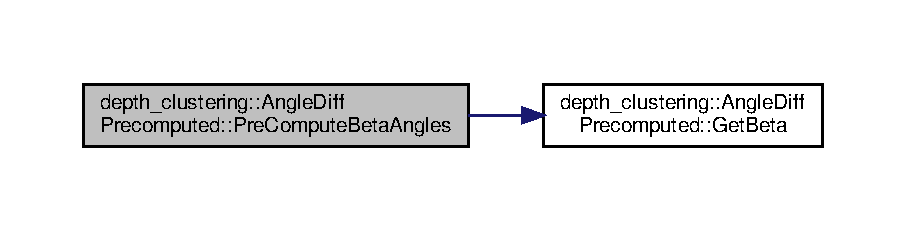
\includegraphics[width=350pt]{classdepth__clustering_1_1AngleDiffPrecomputed_aeb86ee61c6e8fc1b5b554368b1f5fa27_cgraph}
\end{center}
\end{figure}
Here is the caller graph for this function\+:\nopagebreak
\begin{figure}[H]
\begin{center}
\leavevmode
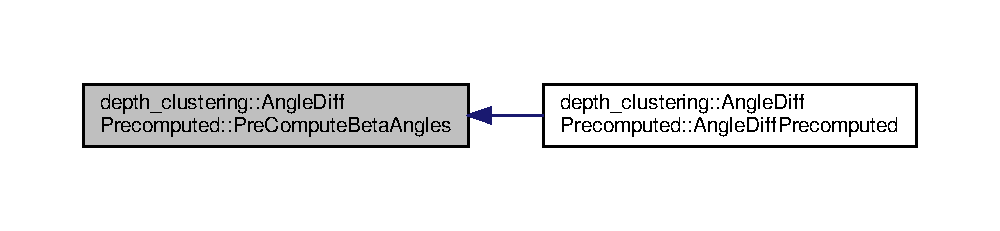
\includegraphics[width=350pt]{classdepth__clustering_1_1AngleDiffPrecomputed_aeb86ee61c6e8fc1b5b554368b1f5fa27_icgraph}
\end{center}
\end{figure}
\mbox{\Hypertarget{classdepth__clustering_1_1AngleDiffPrecomputed_a2fd85404d06843af0ee5c713017f6641}\label{classdepth__clustering_1_1AngleDiffPrecomputed_a2fd85404d06843af0ee5c713017f6641}} 
\index{depth\+\_\+clustering\+::\+Angle\+Diff\+Precomputed@{depth\+\_\+clustering\+::\+Angle\+Diff\+Precomputed}!Visualize@{Visualize}}
\index{Visualize@{Visualize}!depth\+\_\+clustering\+::\+Angle\+Diff\+Precomputed@{depth\+\_\+clustering\+::\+Angle\+Diff\+Precomputed}}
\subsubsection{\texorpdfstring{Visualize()}{Visualize()}}
{\footnotesize\ttfamily cv\+::\+Mat depth\+\_\+clustering\+::\+Angle\+Diff\+Precomputed\+::\+Visualize (\begin{DoxyParamCaption}{ }\end{DoxyParamCaption}) const\hspace{0.3cm}{\ttfamily [virtual]}}



Visualize $\beta$ angles as a {\ttfamily cv\+::\+Mat} color image. 

\begin{DoxyReturn}{Returns}
{\ttfamily cv\+::\+Mat} color image with red channel showing $\beta$ angles in row direction and green channel in col direction. 
\end{DoxyReturn}


Reimplemented from \hyperlink{classdepth__clustering_1_1AbstractDiff_a45314bf711f35e53590af28bdfc45313}{depth\+\_\+clustering\+::\+Abstract\+Diff}.



The documentation for this class was generated from the following files\+:\begin{DoxyCompactItemize}
\item 
/home/ashwin/catkin\+\_\+ws/src/depth\+\_\+clustering/src/image\+\_\+labelers/diff\+\_\+helpers/angle\+\_\+diff.\+h\item 
/home/ashwin/catkin\+\_\+ws/src/depth\+\_\+clustering/src/image\+\_\+labelers/diff\+\_\+helpers/angle\+\_\+diff.\+cpp\end{DoxyCompactItemize}

\hypertarget{classBbox}{}\section{Bbox Class Reference}
\label{classBbox}\index{Bbox@{Bbox}}


Class for bounding box.  




{\ttfamily \#include $<$bbox.\+h$>$}

\subsection*{Public Member Functions}
\begin{DoxyCompactItemize}
\item 
\mbox{\Hypertarget{classBbox_a5d3657403fc62105d71327d50b753ea0}\label{classBbox_a5d3657403fc62105d71327d50b753ea0}} 
{\bfseries Bbox} (const \hyperlink{classdepth__clustering_1_1Cloud}{depth\+\_\+clustering\+::\+Cloud} \&cloud)
\item 
\mbox{\Hypertarget{classBbox_a4aabeabfb52b97da8ce23393d682ca97}\label{classBbox_a4aabeabfb52b97da8ce23393d682ca97}} 
{\bfseries Bbox} (const Eigen\+::\+Vector3f \&min\+\_\+point, const Eigen\+::\+Vector3f \&max\+\_\+point)
\item 
bool \hyperlink{classBbox_a6ac93cd8475f5ef8eb4007d8c206b39d}{Intersects} (const \hyperlink{classBbox}{Bbox} \&other) const
\begin{DoxyCompactList}\small\item\em Check if this bounding box intersects another one. \end{DoxyCompactList}\item 
\hyperlink{classBbox}{Bbox} \hyperlink{classBbox_a0b8e77b794311da86b4c09ed2919af0f}{Intersect} (const \hyperlink{classBbox}{Bbox} \&other) const
\begin{DoxyCompactList}\small\item\em Find the bounding box of the intersection of two boxes. \end{DoxyCompactList}\item 
void \hyperlink{classBbox_ac590fb2bfb031f1ac4238455caf357d7}{Move\+By} (const \hyperlink{classdepth__clustering_1_1Pose}{dc\+::\+Pose} \&pose)
\begin{DoxyCompactList}\small\item\em Return volume of the bounding box. \end{DoxyCompactList}\item 
\mbox{\Hypertarget{classBbox_afdb30a48b141d8905d05ef5d27983a71}\label{classBbox_afdb30a48b141d8905d05ef5d27983a71}} 
float {\bfseries volume} () const
\item 
\mbox{\Hypertarget{classBbox_aeea52d94952b3b0d6eb95eb7e9bdfa60}\label{classBbox_aeea52d94952b3b0d6eb95eb7e9bdfa60}} 
Eigen\+::\+Vector3f {\bfseries center} () const
\item 
\mbox{\Hypertarget{classBbox_adbd4cd66414ec9dd99a64dcc7fefa0eb}\label{classBbox_adbd4cd66414ec9dd99a64dcc7fefa0eb}} 
Eigen\+::\+Vector3f {\bfseries scale} () const
\item 
\mbox{\Hypertarget{classBbox_acabe3355373b58b56070fd1ead9fdef7}\label{classBbox_acabe3355373b58b56070fd1ead9fdef7}} 
const Eigen\+::\+Vector3f \& {\bfseries min\+\_\+point} () const
\item 
\mbox{\Hypertarget{classBbox_a9c1593c5debe2ab4d9308d56b4a4fa99}\label{classBbox_a9c1593c5debe2ab4d9308d56b4a4fa99}} 
const Eigen\+::\+Vector3f \& {\bfseries max\+\_\+point} () const
\item 
\mbox{\Hypertarget{classBbox_af31d201dfcf52443564e4a2e028008bd}\label{classBbox_af31d201dfcf52443564e4a2e028008bd}} 
float {\bfseries Get\+ScaleX} () const
\item 
\mbox{\Hypertarget{classBbox_a819de405229a7113aa1f55fc9a5e10a1}\label{classBbox_a819de405229a7113aa1f55fc9a5e10a1}} 
float {\bfseries Get\+ScaleY} () const
\item 
\mbox{\Hypertarget{classBbox_a80b58db650bee5a4ea7cfb6205aeab49}\label{classBbox_a80b58db650bee5a4ea7cfb6205aeab49}} 
float {\bfseries Get\+ScaleZ} () const
\item 
\mbox{\Hypertarget{classBbox_aee6dac16a8833cb9a608a0fdafaf9772}\label{classBbox_aee6dac16a8833cb9a608a0fdafaf9772}} 
void {\bfseries Update\+Scale\+And\+Center} ()
\end{DoxyCompactItemize}
\subsection*{Static Public Attributes}
\begin{DoxyCompactItemize}
\item 
\mbox{\Hypertarget{classBbox_a42eb77afd3b8b1c32869c01ecf073bc3}\label{classBbox_a42eb77afd3b8b1c32869c01ecf073bc3}} 
static constexpr float {\bfseries W\+R\+O\+N\+G\+\_\+\+V\+O\+L\+U\+ME} = -\/1.\+0f
\end{DoxyCompactItemize}


\subsection{Detailed Description}
Class for bounding box. 

Collaboration diagram for Bbox\+:\nopagebreak
\begin{figure}[H]
\begin{center}
\leavevmode
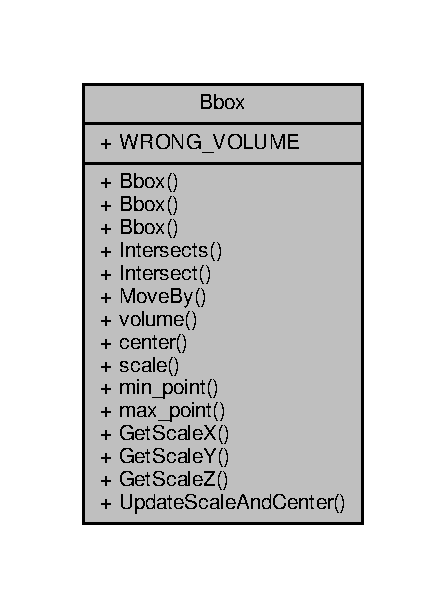
\includegraphics[width=214pt]{classBbox__coll__graph}
\end{center}
\end{figure}


\subsection{Member Function Documentation}
\mbox{\Hypertarget{classBbox_a0b8e77b794311da86b4c09ed2919af0f}\label{classBbox_a0b8e77b794311da86b4c09ed2919af0f}} 
\index{Bbox@{Bbox}!Intersect@{Intersect}}
\index{Intersect@{Intersect}!Bbox@{Bbox}}
\subsubsection{\texorpdfstring{Intersect()}{Intersect()}}
{\footnotesize\ttfamily \hyperlink{classBbox}{Bbox} Bbox\+::\+Intersect (\begin{DoxyParamCaption}\item[{const \hyperlink{classBbox}{Bbox} \&}]{other }\end{DoxyParamCaption}) const}



Find the bounding box of the intersection of two boxes. 


\begin{DoxyParams}[1]{Parameters}
\mbox{\tt in}  & {\em other} & The other bounding box.\\
\hline
\end{DoxyParams}
\begin{DoxyReturn}{Returns}
A bounding box of the intersection. 
\end{DoxyReturn}
Here is the caller graph for this function\+:\nopagebreak
\begin{figure}[H]
\begin{center}
\leavevmode
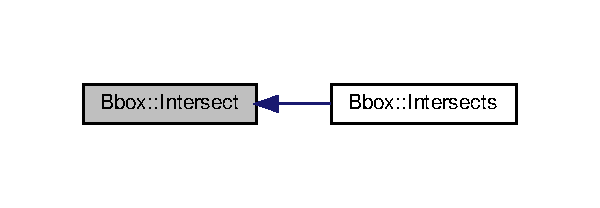
\includegraphics[width=288pt]{classBbox_a0b8e77b794311da86b4c09ed2919af0f_icgraph}
\end{center}
\end{figure}
\mbox{\Hypertarget{classBbox_a6ac93cd8475f5ef8eb4007d8c206b39d}\label{classBbox_a6ac93cd8475f5ef8eb4007d8c206b39d}} 
\index{Bbox@{Bbox}!Intersects@{Intersects}}
\index{Intersects@{Intersects}!Bbox@{Bbox}}
\subsubsection{\texorpdfstring{Intersects()}{Intersects()}}
{\footnotesize\ttfamily bool Bbox\+::\+Intersects (\begin{DoxyParamCaption}\item[{const \hyperlink{classBbox}{Bbox} \&}]{other }\end{DoxyParamCaption}) const}



Check if this bounding box intersects another one. 


\begin{DoxyParams}[1]{Parameters}
\mbox{\tt in}  & {\em other} & The other bounding box.\\
\hline
\end{DoxyParams}
\begin{DoxyReturn}{Returns}
true if intersects, false otherwise 
\end{DoxyReturn}
Here is the call graph for this function\+:\nopagebreak
\begin{figure}[H]
\begin{center}
\leavevmode
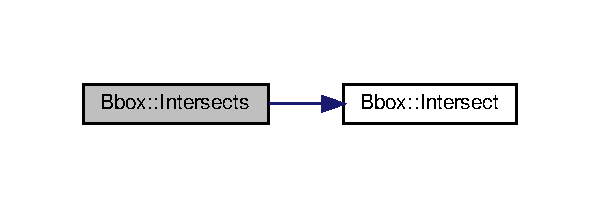
\includegraphics[width=288pt]{classBbox_a6ac93cd8475f5ef8eb4007d8c206b39d_cgraph}
\end{center}
\end{figure}
\mbox{\Hypertarget{classBbox_ac590fb2bfb031f1ac4238455caf357d7}\label{classBbox_ac590fb2bfb031f1ac4238455caf357d7}} 
\index{Bbox@{Bbox}!Move\+By@{Move\+By}}
\index{Move\+By@{Move\+By}!Bbox@{Bbox}}
\subsubsection{\texorpdfstring{Move\+By()}{MoveBy()}}
{\footnotesize\ttfamily void Bbox\+::\+Move\+By (\begin{DoxyParamCaption}\item[{const \hyperlink{classdepth__clustering_1_1Pose}{dc\+::\+Pose} \&}]{pose }\end{DoxyParamCaption})\hspace{0.3cm}{\ttfamily [inline]}}



Return volume of the bounding box. 

\begin{DoxyReturn}{Returns}
Volume of the bounding box. 
\end{DoxyReturn}


The documentation for this class was generated from the following files\+:\begin{DoxyCompactItemize}
\item 
/home/ashwin/catkin\+\_\+ws/src/depth\+\_\+clustering/src/utils/bbox.\+h\item 
/home/ashwin/catkin\+\_\+ws/src/depth\+\_\+clustering/src/utils/bbox.\+cpp\end{DoxyCompactItemize}

\hypertarget{classdepth__clustering_1_1Cloud}{}\section{depth\+\_\+clustering\+:\+:Cloud Class Reference}
\label{classdepth__clustering_1_1Cloud}\index{depth\+\_\+clustering\+::\+Cloud@{depth\+\_\+clustering\+::\+Cloud}}


A class that stores a vector of Rich\+Points.  




{\ttfamily \#include $<$cloud.\+h$>$}

\subsection*{Public Types}
\begin{DoxyCompactItemize}
\item 
\mbox{\Hypertarget{classdepth__clustering_1_1Cloud_a6357719aeeb7c05cbd4a375f63526ba1}\label{classdepth__clustering_1_1Cloud_a6357719aeeb7c05cbd4a375f63526ba1}} 
using {\bfseries Ptr} = shared\+\_\+ptr$<$ \hyperlink{classdepth__clustering_1_1Cloud}{Cloud} $>$
\item 
\mbox{\Hypertarget{classdepth__clustering_1_1Cloud_ae8ba86a4493a06d04e25cba4e97b9787}\label{classdepth__clustering_1_1Cloud_ae8ba86a4493a06d04e25cba4e97b9787}} 
using {\bfseries Const\+Ptr} = shared\+\_\+ptr$<$ const \hyperlink{classdepth__clustering_1_1Cloud}{Cloud} $>$
\end{DoxyCompactItemize}
\subsection*{Public Member Functions}
\begin{DoxyCompactItemize}
\item 
\mbox{\Hypertarget{classdepth__clustering_1_1Cloud_a00490840c02e90434727d71718323d11}\label{classdepth__clustering_1_1Cloud_a00490840c02e90434727d71718323d11}} 
{\bfseries Cloud} (const \hyperlink{classdepth__clustering_1_1Cloud}{Cloud} \&cloud)
\item 
\mbox{\Hypertarget{classdepth__clustering_1_1Cloud_abbb28f15b4cb992ef8c685d8ac74497c}\label{classdepth__clustering_1_1Cloud_abbb28f15b4cb992ef8c685d8ac74497c}} 
{\bfseries Cloud} (const \hyperlink{classdepth__clustering_1_1Pose}{Pose} \&pose)
\item 
\mbox{\Hypertarget{classdepth__clustering_1_1Cloud_a16d2ddc6cf2af152c8e5ef2b71f059e4}\label{classdepth__clustering_1_1Cloud_a16d2ddc6cf2af152c8e5ef2b71f059e4}} 
const Rich\+Point\+::\+Aligned\+Vector \& {\bfseries points} () const
\item 
\mbox{\Hypertarget{classdepth__clustering_1_1Cloud_a549f7235008ad6e404989ebb621d3d16}\label{classdepth__clustering_1_1Cloud_a549f7235008ad6e404989ebb621d3d16}} 
\hyperlink{classdepth__clustering_1_1Pose}{Pose} \& {\bfseries pose} ()
\item 
\mbox{\Hypertarget{classdepth__clustering_1_1Cloud_a235dc6b26381d20d7cd57d80837e3f93}\label{classdepth__clustering_1_1Cloud_a235dc6b26381d20d7cd57d80837e3f93}} 
const \hyperlink{classdepth__clustering_1_1Pose}{Pose} \& {\bfseries pose} () const
\item 
\mbox{\Hypertarget{classdepth__clustering_1_1Cloud_a8aeb9afd4c1b7da85f79f7eb2e4bd432}\label{classdepth__clustering_1_1Cloud_a8aeb9afd4c1b7da85f79f7eb2e4bd432}} 
\hyperlink{classdepth__clustering_1_1Pose}{Pose} \& {\bfseries sensor\+\_\+pose} ()
\item 
\mbox{\Hypertarget{classdepth__clustering_1_1Cloud_af671b5d52f019d532874e5189ba3d135}\label{classdepth__clustering_1_1Cloud_af671b5d52f019d532874e5189ba3d135}} 
const \hyperlink{classdepth__clustering_1_1Pose}{Pose} \& {\bfseries sensor\+\_\+pose} () const
\item 
\mbox{\Hypertarget{classdepth__clustering_1_1Cloud_a3cb61254a6c969d22810b2097f59b4cf}\label{classdepth__clustering_1_1Cloud_a3cb61254a6c969d22810b2097f59b4cf}} 
void {\bfseries push\+\_\+back} (const \hyperlink{classdepth__clustering_1_1RichPoint}{Rich\+Point} \&point)
\item 
\mbox{\Hypertarget{classdepth__clustering_1_1Cloud_ad716661e0b53d51df13576480714beef}\label{classdepth__clustering_1_1Cloud_ad716661e0b53d51df13576480714beef}} 
size\+\_\+t {\bfseries size} () const
\item 
\mbox{\Hypertarget{classdepth__clustering_1_1Cloud_a6713820e4633e1f460c99e47e9aeaf96}\label{classdepth__clustering_1_1Cloud_a6713820e4633e1f460c99e47e9aeaf96}} 
bool {\bfseries empty} () const
\item 
\mbox{\Hypertarget{classdepth__clustering_1_1Cloud_ac92794f086743a2fbc025c168d1ac846}\label{classdepth__clustering_1_1Cloud_ac92794f086743a2fbc025c168d1ac846}} 
void {\bfseries reserve} (size\+\_\+t size)
\item 
\mbox{\Hypertarget{classdepth__clustering_1_1Cloud_aeb0d22cf0ace96f36d9f74f6bf9bfa47}\label{classdepth__clustering_1_1Cloud_aeb0d22cf0ace96f36d9f74f6bf9bfa47}} 
\hyperlink{classdepth__clustering_1_1RichPoint}{Rich\+Point} \& {\bfseries operator\mbox{[}$\,$\mbox{]}} (int idx)
\item 
\mbox{\Hypertarget{classdepth__clustering_1_1Cloud_ae755d1933404025686e0f6d12c55ecf2}\label{classdepth__clustering_1_1Cloud_ae755d1933404025686e0f6d12c55ecf2}} 
const \hyperlink{classdepth__clustering_1_1RichPoint}{Rich\+Point} \& {\bfseries operator\mbox{[}$\,$\mbox{]}} (int idx) const
\item 
\mbox{\Hypertarget{classdepth__clustering_1_1Cloud_a91cca0639df32d3b4ceed11e7baf8988}\label{classdepth__clustering_1_1Cloud_a91cca0639df32d3b4ceed11e7baf8988}} 
\hyperlink{classdepth__clustering_1_1RichPoint}{Rich\+Point} \& {\bfseries at} (int idx)
\item 
\mbox{\Hypertarget{classdepth__clustering_1_1Cloud_aae9b5275a575fa233750553a5ce0e55a}\label{classdepth__clustering_1_1Cloud_aae9b5275a575fa233750553a5ce0e55a}} 
const \hyperlink{classdepth__clustering_1_1RichPoint}{Rich\+Point} \& {\bfseries at} (int idx) const
\item 
\mbox{\Hypertarget{classdepth__clustering_1_1Cloud_a2d25f4ec2e3d45016ecd7fa715273624}\label{classdepth__clustering_1_1Cloud_a2d25f4ec2e3d45016ecd7fa715273624}} 
void {\bfseries Resize} (size\+\_\+t new\+\_\+size)
\item 
\mbox{\Hypertarget{classdepth__clustering_1_1Cloud_a2a5b5ba64b5e2cdfaf3f1418962fa93f}\label{classdepth__clustering_1_1Cloud_a2a5b5ba64b5e2cdfaf3f1418962fa93f}} 
void {\bfseries Set\+Pose} (const \hyperlink{classdepth__clustering_1_1Pose}{Pose} \&pose)
\item 
\mbox{\Hypertarget{classdepth__clustering_1_1Cloud_a6ac41fa70ba489c0784b197350668ec4}\label{classdepth__clustering_1_1Cloud_a6ac41fa70ba489c0784b197350668ec4}} 
const Cloud\+Projection\+::\+Const\+Ptr {\bfseries projection\+\_\+ptr} () const
\item 
\mbox{\Hypertarget{classdepth__clustering_1_1Cloud_ac973b1445bd435f0f2df0dc06b654f07}\label{classdepth__clustering_1_1Cloud_ac973b1445bd435f0f2df0dc06b654f07}} 
Cloud\+Projection\+::\+Ptr {\bfseries projection\+\_\+ptr} ()
\item 
\mbox{\Hypertarget{classdepth__clustering_1_1Cloud_a8821b4a97d1f8b4e6415731f3e2b2f89}\label{classdepth__clustering_1_1Cloud_a8821b4a97d1f8b4e6415731f3e2b2f89}} 
std\+::list$<$ const \hyperlink{classdepth__clustering_1_1RichPoint}{Rich\+Point} $\ast$ $>$ {\bfseries Points\+Projected\+To\+Pixel} (int row, int col) const
\item 
\mbox{\Hypertarget{classdepth__clustering_1_1Cloud_a448638dcb9f8e5a17370ba81e9e80d68}\label{classdepth__clustering_1_1Cloud_a448638dcb9f8e5a17370ba81e9e80d68}} 
void {\bfseries Transform\+In\+Place} (const \hyperlink{classdepth__clustering_1_1Pose}{Pose} \&pose)
\item 
\mbox{\Hypertarget{classdepth__clustering_1_1Cloud_a93a9d173055f3a624db2fe4b1345eb13}\label{classdepth__clustering_1_1Cloud_a93a9d173055f3a624db2fe4b1345eb13}} 
Cloud\+::\+Ptr {\bfseries Transform} (const \hyperlink{classdepth__clustering_1_1Pose}{Pose} \&pose) const
\item 
\mbox{\Hypertarget{classdepth__clustering_1_1Cloud_abc1dcb82d072a45e8c00170cc927f537}\label{classdepth__clustering_1_1Cloud_abc1dcb82d072a45e8c00170cc927f537}} 
void {\bfseries Set\+Projection\+Ptr} (typename Cloud\+Projection\+::\+Ptr proj\+\_\+ptr)
\item 
\mbox{\Hypertarget{classdepth__clustering_1_1Cloud_a052108fe3780dec4209b80e8b7886457}\label{classdepth__clustering_1_1Cloud_a052108fe3780dec4209b80e8b7886457}} 
void {\bfseries Init\+Projection} (const \hyperlink{classdepth__clustering_1_1ProjectionParams}{Projection\+Params} \&params)
\end{DoxyCompactItemize}
\subsection*{Static Public Member Functions}
\begin{DoxyCompactItemize}
\item 
\mbox{\Hypertarget{classdepth__clustering_1_1Cloud_a30f8b04595f44fc56d42f556efbebe7f}\label{classdepth__clustering_1_1Cloud_a30f8b04595f44fc56d42f556efbebe7f}} 
static Cloud\+::\+Ptr {\bfseries From\+Image} (const cv\+::\+Mat \&image, const \hyperlink{classdepth__clustering_1_1ProjectionParams}{Projection\+Params} \&params)
\end{DoxyCompactItemize}
\subsection*{Protected Attributes}
\begin{DoxyCompactItemize}
\item 
\mbox{\Hypertarget{classdepth__clustering_1_1Cloud_a6827950219a447bb1d3c390168d3397d}\label{classdepth__clustering_1_1Cloud_a6827950219a447bb1d3c390168d3397d}} 
Rich\+Point\+::\+Aligned\+Vector {\bfseries \+\_\+points}
\item 
\mbox{\Hypertarget{classdepth__clustering_1_1Cloud_a3b6a1ada445763ab4b9ac9519bb225f1}\label{classdepth__clustering_1_1Cloud_a3b6a1ada445763ab4b9ac9519bb225f1}} 
\hyperlink{classdepth__clustering_1_1Pose}{Pose} {\bfseries \+\_\+pose}
\item 
\mbox{\Hypertarget{classdepth__clustering_1_1Cloud_a6399645406eaa1312ca4a469d7c4db1f}\label{classdepth__clustering_1_1Cloud_a6399645406eaa1312ca4a469d7c4db1f}} 
\hyperlink{classdepth__clustering_1_1Pose}{Pose} {\bfseries \+\_\+sensor\+\_\+pose}
\item 
\mbox{\Hypertarget{classdepth__clustering_1_1Cloud_a5f60147c48b39a951d4fa72ba60ef370}\label{classdepth__clustering_1_1Cloud_a5f60147c48b39a951d4fa72ba60ef370}} 
Cloud\+Projection\+::\+Ptr {\bfseries \+\_\+projection} = nullptr
\end{DoxyCompactItemize}


\subsection{Detailed Description}
A class that stores a vector of Rich\+Points. 

A utility class for storing points. If P\+CL is available has ways of converting to and from pcl. Also knows how to generate a projection from its points and can be generated from an image. 

Collaboration diagram for depth\+\_\+clustering\+:\+:Cloud\+:\nopagebreak
\begin{figure}[H]
\begin{center}
\leavevmode
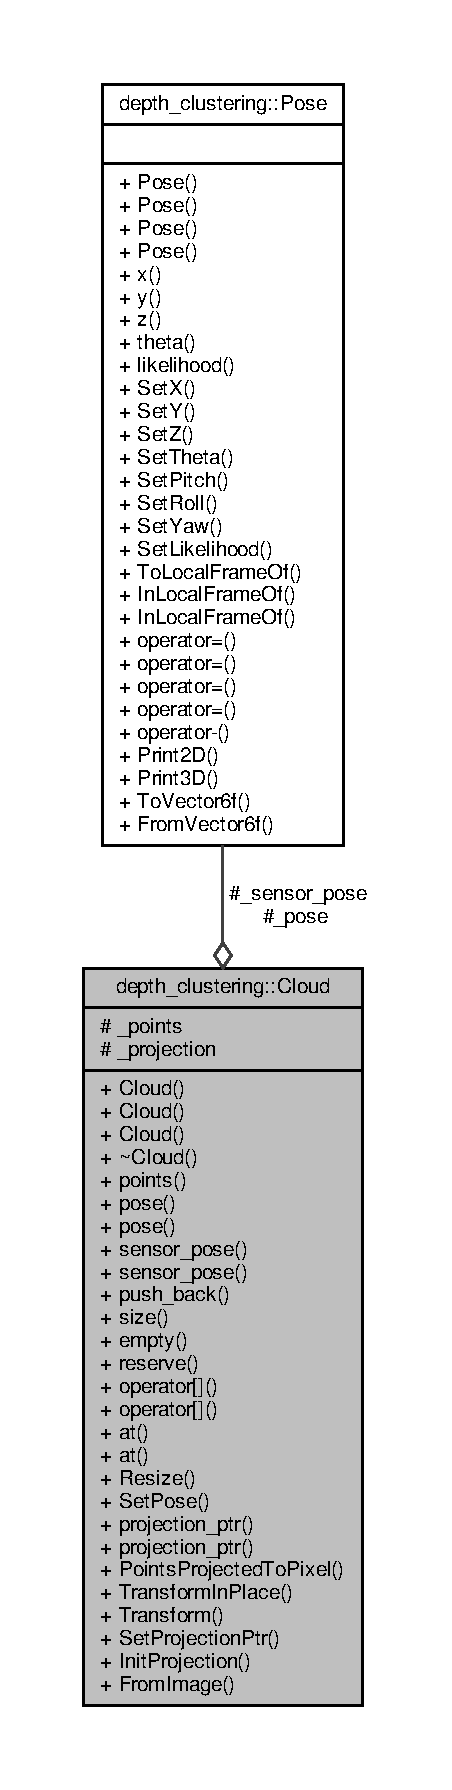
\includegraphics[height=550pt]{classdepth__clustering_1_1Cloud__coll__graph}
\end{center}
\end{figure}


The documentation for this class was generated from the following files\+:\begin{DoxyCompactItemize}
\item 
/home/ashwin/catkin\+\_\+ws/src/depth\+\_\+clustering/src/utils/cloud.\+h\item 
/home/ashwin/catkin\+\_\+ws/src/depth\+\_\+clustering/src/utils/cloud.\+cpp\end{DoxyCompactItemize}

\hypertarget{classdepth__clustering_1_1CloudOdomRosSubscriber}{}\section{depth\+\_\+clustering\+:\+:Cloud\+Odom\+Ros\+Subscriber Class Reference}
\label{classdepth__clustering_1_1CloudOdomRosSubscriber}\index{depth\+\_\+clustering\+::\+Cloud\+Odom\+Ros\+Subscriber@{depth\+\_\+clustering\+::\+Cloud\+Odom\+Ros\+Subscriber}}


Class for cloud odom ros subscriber.  




{\ttfamily \#include $<$cloud\+\_\+odom\+\_\+ros\+\_\+subscriber.\+h$>$}

\subsection*{Public Member Functions}
\begin{DoxyCompactItemize}
\item 
\mbox{\Hypertarget{classdepth__clustering_1_1CloudOdomRosSubscriber_a01d66910b5dfe1d1145a8d68645bd7b4}\label{classdepth__clustering_1_1CloudOdomRosSubscriber_a01d66910b5dfe1d1145a8d68645bd7b4}} 
{\bfseries Cloud\+Odom\+Ros\+Subscriber} (ros\+::\+Node\+Handle $\ast$node\+\_\+handle, const \hyperlink{classdepth__clustering_1_1ProjectionParams}{Projection\+Params} \&params, const std\+::string \&topic\+\_\+clouds, const std\+::string \&topic\+\_\+odom=\char`\"{}\char`\"{})
\item 
void \hyperlink{classdepth__clustering_1_1CloudOdomRosSubscriber_a76a7474f1deed190ac2fb57084c4cdb9}{Callback} (const Point\+Cloud\+T\+::\+Const\+Ptr \&msg\+\_\+cloud, const Odometry\+T\+::\+Const\+Ptr \&msg\+\_\+odom)
\begin{DoxyCompactList}\small\item\em Get synchronized odometry and cloud. \end{DoxyCompactList}\item 
void \hyperlink{classdepth__clustering_1_1CloudOdomRosSubscriber_a8de806bc0b847229dcc92c504908f019}{Callback\+Velodyne} (const sensor\+\_\+msgs\+::\+Point\+Cloud2\+::\+Const\+Ptr \&msg\+\_\+cloud)
\begin{DoxyCompactList}\small\item\em Get point cloud from R\+OS. \end{DoxyCompactList}\item 
\mbox{\Hypertarget{classdepth__clustering_1_1CloudOdomRosSubscriber_a16020c63b14308591cae6f4a9ba9b29a}\label{classdepth__clustering_1_1CloudOdomRosSubscriber_a16020c63b14308591cae6f4a9ba9b29a}} 
void \hyperlink{classdepth__clustering_1_1CloudOdomRosSubscriber_a16020c63b14308591cae6f4a9ba9b29a}{Start\+Listening\+To\+Ros} ()
\begin{DoxyCompactList}\small\item\em Starts listening to ros. \end{DoxyCompactList}\end{DoxyCompactItemize}
\subsection*{Protected Member Functions}
\begin{DoxyCompactItemize}
\item 
\mbox{\Hypertarget{classdepth__clustering_1_1CloudOdomRosSubscriber_a2a5fac22f067b9cbfd395814c6939d8a}\label{classdepth__clustering_1_1CloudOdomRosSubscriber_a2a5fac22f067b9cbfd395814c6939d8a}} 
\hyperlink{classdepth__clustering_1_1Pose}{Pose} {\bfseries Ros\+Odom\+To\+Pose} (const Odometry\+T\+::\+Const\+Ptr \&msg)
\item 
\mbox{\Hypertarget{classdepth__clustering_1_1CloudOdomRosSubscriber_ad80bb8e5ba1f5f21221233145337c5eb}\label{classdepth__clustering_1_1CloudOdomRosSubscriber_ad80bb8e5ba1f5f21221233145337c5eb}} 
Cloud\+::\+Ptr {\bfseries Ros\+Cloud\+To\+Cloud} (const Point\+Cloud\+T\+::\+Const\+Ptr \&msg)
\end{DoxyCompactItemize}
\subsection*{Protected Attributes}
\begin{DoxyCompactItemize}
\item 
\mbox{\Hypertarget{classdepth__clustering_1_1CloudOdomRosSubscriber_af44b4e9d0bfe1c030324ea4600a8d49e}\label{classdepth__clustering_1_1CloudOdomRosSubscriber_af44b4e9d0bfe1c030324ea4600a8d49e}} 
ros\+::\+Node\+Handle $\ast$ {\bfseries \+\_\+node\+\_\+handle}
\item 
\mbox{\Hypertarget{classdepth__clustering_1_1CloudOdomRosSubscriber_a47a509c60650a113d7aba3a36c7a6a17}\label{classdepth__clustering_1_1CloudOdomRosSubscriber_a47a509c60650a113d7aba3a36c7a6a17}} 
message\+\_\+filters\+::\+Subscriber$<$ Point\+CloudT $>$ $\ast$ {\bfseries \+\_\+subscriber\+\_\+clouds}
\item 
\mbox{\Hypertarget{classdepth__clustering_1_1CloudOdomRosSubscriber_a869ac4843118077f95777dc483d13873}\label{classdepth__clustering_1_1CloudOdomRosSubscriber_a869ac4843118077f95777dc483d13873}} 
message\+\_\+filters\+::\+Subscriber$<$ OdometryT $>$ $\ast$ {\bfseries \+\_\+subscriber\+\_\+odom}
\item 
\mbox{\Hypertarget{classdepth__clustering_1_1CloudOdomRosSubscriber_a4829e587d2ae9c5fee5e3cf753cdeee9}\label{classdepth__clustering_1_1CloudOdomRosSubscriber_a4829e587d2ae9c5fee5e3cf753cdeee9}} 
message\+\_\+filters\+::\+Synchronizer$<$ Approximate\+Time\+Policy $>$ $\ast$ {\bfseries \+\_\+sync}
\item 
\mbox{\Hypertarget{classdepth__clustering_1_1CloudOdomRosSubscriber_ac172f353e2f6fec4d8f07b3a431048a1}\label{classdepth__clustering_1_1CloudOdomRosSubscriber_ac172f353e2f6fec4d8f07b3a431048a1}} 
std\+::string {\bfseries \+\_\+topic\+\_\+clouds}
\item 
\mbox{\Hypertarget{classdepth__clustering_1_1CloudOdomRosSubscriber_ad1c0dcb17a16f5611d13afb8e76656e5}\label{classdepth__clustering_1_1CloudOdomRosSubscriber_ad1c0dcb17a16f5611d13afb8e76656e5}} 
std\+::string {\bfseries \+\_\+topic\+\_\+odom}
\item 
\mbox{\Hypertarget{classdepth__clustering_1_1CloudOdomRosSubscriber_a0661d98cffa781b355209e71075983b1}\label{classdepth__clustering_1_1CloudOdomRosSubscriber_a0661d98cffa781b355209e71075983b1}} 
\hyperlink{classdepth__clustering_1_1ProjectionParams}{Projection\+Params} {\bfseries \+\_\+params}
\item 
\mbox{\Hypertarget{classdepth__clustering_1_1CloudOdomRosSubscriber_a4d9749a4c49ef4c91807ab2a573e33fe}\label{classdepth__clustering_1_1CloudOdomRosSubscriber_a4d9749a4c49ef4c91807ab2a573e33fe}} 
int {\bfseries \+\_\+msg\+\_\+queue\+\_\+size}
\end{DoxyCompactItemize}
\subsection*{Additional Inherited Members}


\subsection{Detailed Description}
Class for cloud odom ros subscriber. 

Inheritance diagram for depth\+\_\+clustering\+:\+:Cloud\+Odom\+Ros\+Subscriber\+:\nopagebreak
\begin{figure}[H]
\begin{center}
\leavevmode
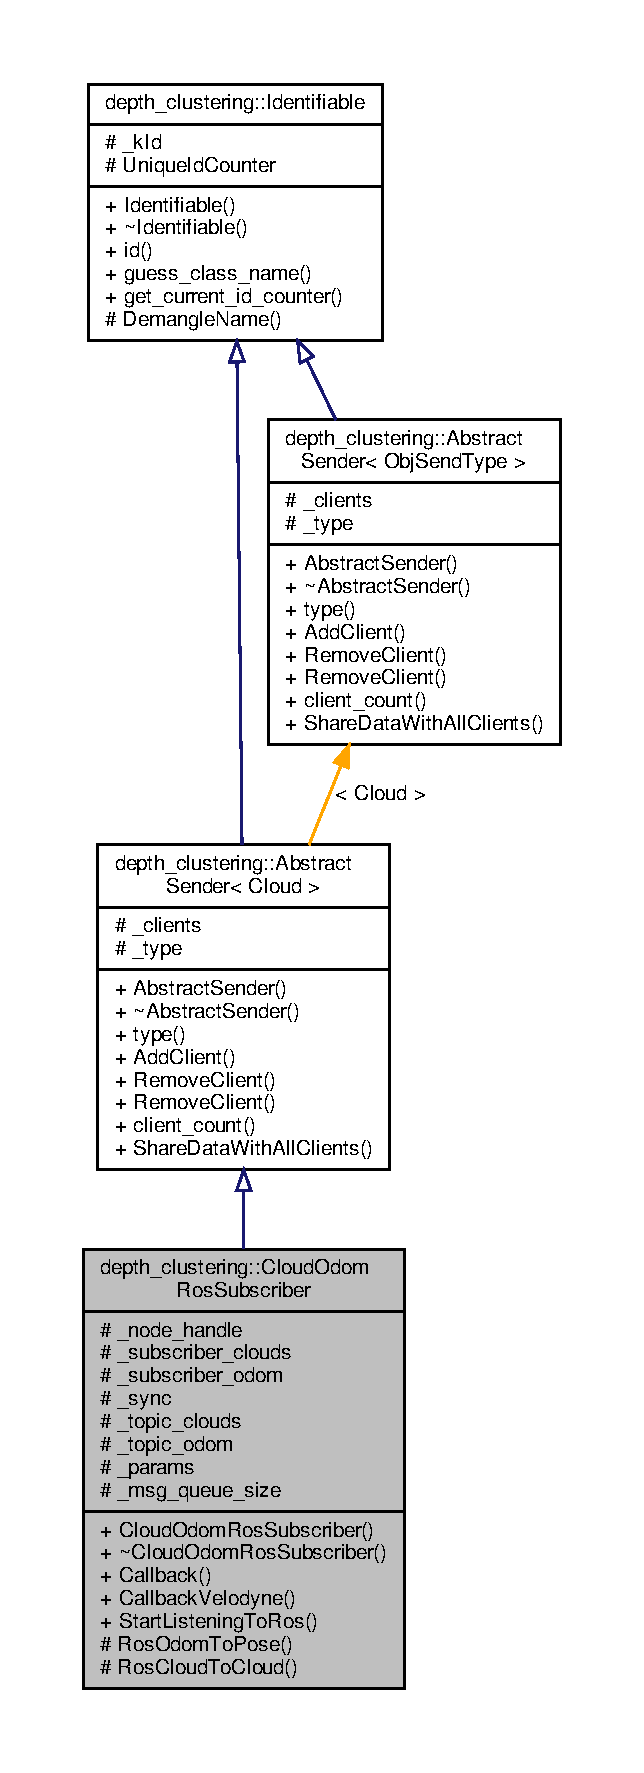
\includegraphics[height=550pt]{classdepth__clustering_1_1CloudOdomRosSubscriber__inherit__graph}
\end{center}
\end{figure}


Collaboration diagram for depth\+\_\+clustering\+:\+:Cloud\+Odom\+Ros\+Subscriber\+:\nopagebreak
\begin{figure}[H]
\begin{center}
\leavevmode
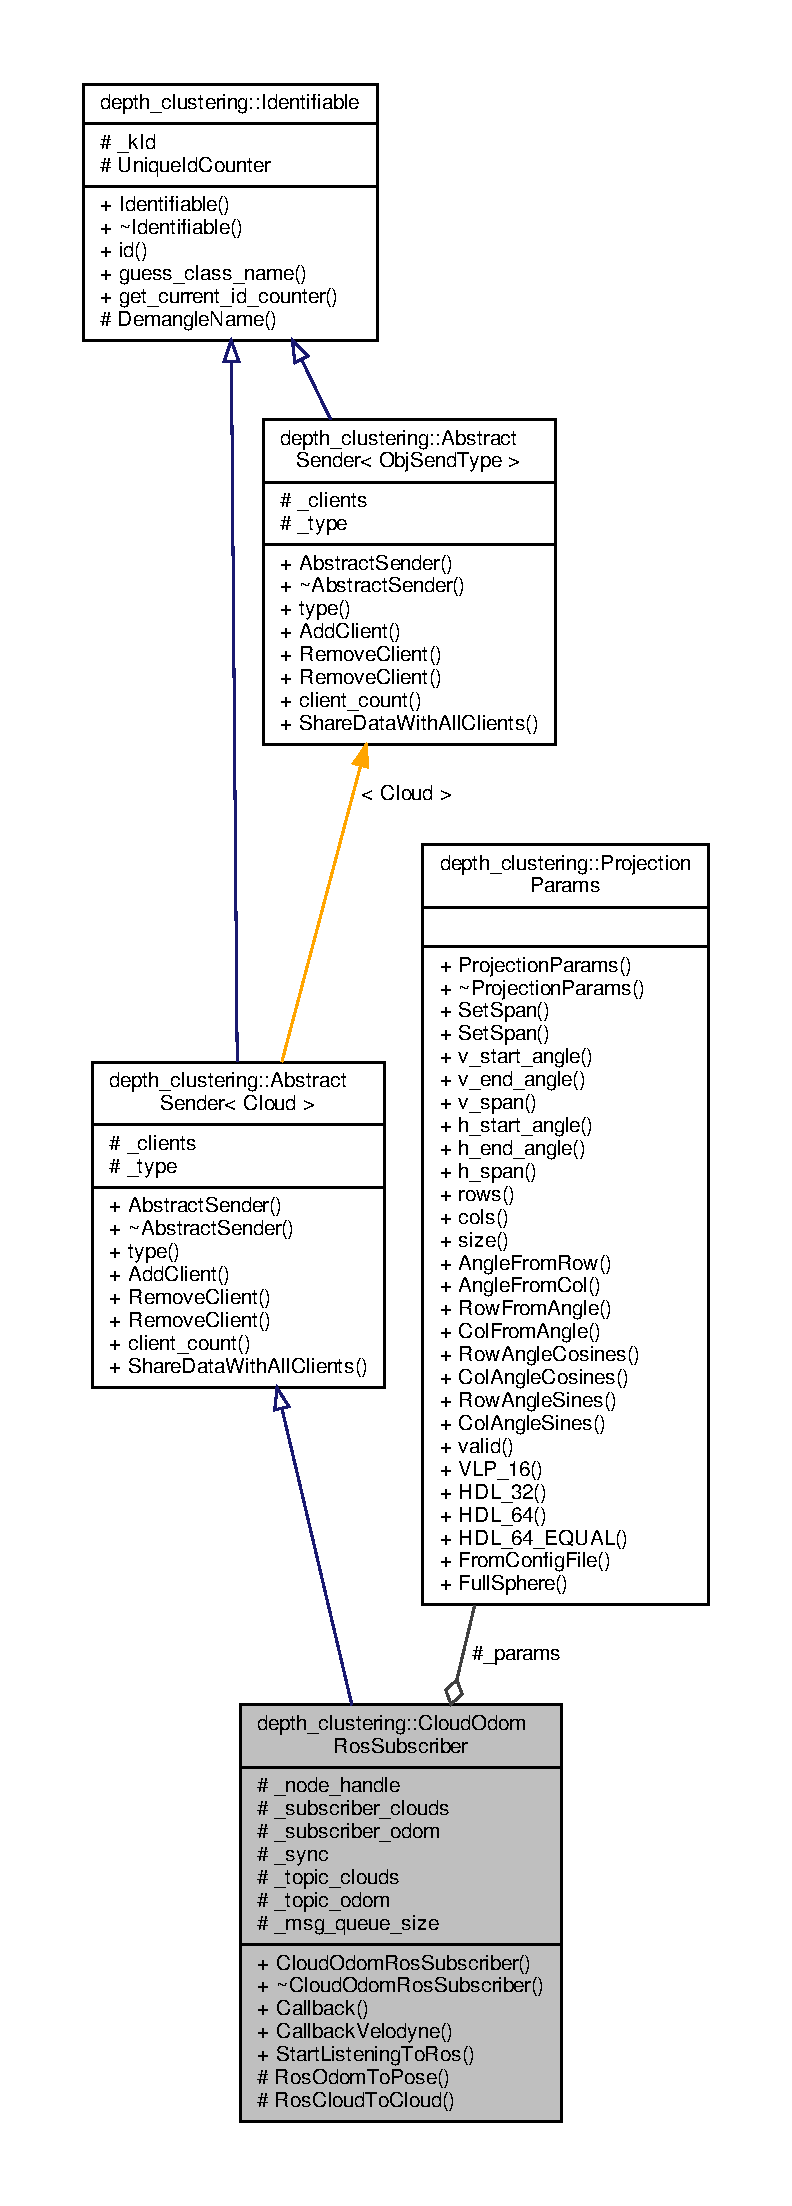
\includegraphics[height=550pt]{classdepth__clustering_1_1CloudOdomRosSubscriber__coll__graph}
\end{center}
\end{figure}


\subsection{Member Function Documentation}
\mbox{\Hypertarget{classdepth__clustering_1_1CloudOdomRosSubscriber_a76a7474f1deed190ac2fb57084c4cdb9}\label{classdepth__clustering_1_1CloudOdomRosSubscriber_a76a7474f1deed190ac2fb57084c4cdb9}} 
\index{depth\+\_\+clustering\+::\+Cloud\+Odom\+Ros\+Subscriber@{depth\+\_\+clustering\+::\+Cloud\+Odom\+Ros\+Subscriber}!Callback@{Callback}}
\index{Callback@{Callback}!depth\+\_\+clustering\+::\+Cloud\+Odom\+Ros\+Subscriber@{depth\+\_\+clustering\+::\+Cloud\+Odom\+Ros\+Subscriber}}
\subsubsection{\texorpdfstring{Callback()}{Callback()}}
{\footnotesize\ttfamily void depth\+\_\+clustering\+::\+Cloud\+Odom\+Ros\+Subscriber\+::\+Callback (\begin{DoxyParamCaption}\item[{const Point\+Cloud\+T\+::\+Const\+Ptr \&}]{msg\+\_\+cloud,  }\item[{const Odometry\+T\+::\+Const\+Ptr \&}]{msg\+\_\+odom }\end{DoxyParamCaption})}



Get synchronized odometry and cloud. 


\begin{DoxyParams}[1]{Parameters}
\mbox{\tt in}  & {\em msg\+\_\+cloud} & The message cloud \\
\hline
\mbox{\tt in}  & {\em msg\+\_\+odom} & The message odom \\
\hline
\end{DoxyParams}
Here is the caller graph for this function\+:\nopagebreak
\begin{figure}[H]
\begin{center}
\leavevmode
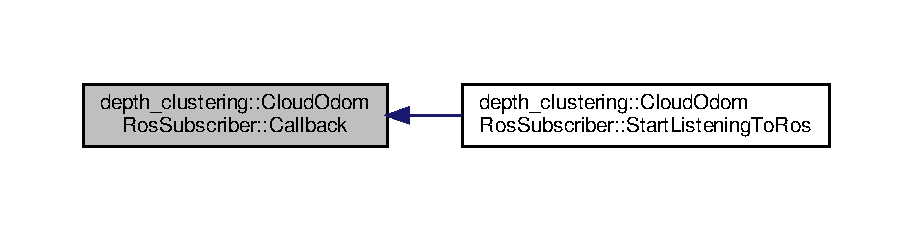
\includegraphics[width=350pt]{classdepth__clustering_1_1CloudOdomRosSubscriber_a76a7474f1deed190ac2fb57084c4cdb9_icgraph}
\end{center}
\end{figure}
\mbox{\Hypertarget{classdepth__clustering_1_1CloudOdomRosSubscriber_a8de806bc0b847229dcc92c504908f019}\label{classdepth__clustering_1_1CloudOdomRosSubscriber_a8de806bc0b847229dcc92c504908f019}} 
\index{depth\+\_\+clustering\+::\+Cloud\+Odom\+Ros\+Subscriber@{depth\+\_\+clustering\+::\+Cloud\+Odom\+Ros\+Subscriber}!Callback\+Velodyne@{Callback\+Velodyne}}
\index{Callback\+Velodyne@{Callback\+Velodyne}!depth\+\_\+clustering\+::\+Cloud\+Odom\+Ros\+Subscriber@{depth\+\_\+clustering\+::\+Cloud\+Odom\+Ros\+Subscriber}}
\subsubsection{\texorpdfstring{Callback\+Velodyne()}{CallbackVelodyne()}}
{\footnotesize\ttfamily void depth\+\_\+clustering\+::\+Cloud\+Odom\+Ros\+Subscriber\+::\+Callback\+Velodyne (\begin{DoxyParamCaption}\item[{const sensor\+\_\+msgs\+::\+Point\+Cloud2\+::\+Const\+Ptr \&}]{msg\+\_\+cloud }\end{DoxyParamCaption})}



Get point cloud from R\+OS. 


\begin{DoxyParams}[1]{Parameters}
\mbox{\tt in}  & {\em msg\+\_\+cloud} & The message cloud \\
\hline
\end{DoxyParams}
Here is the caller graph for this function\+:\nopagebreak
\begin{figure}[H]
\begin{center}
\leavevmode
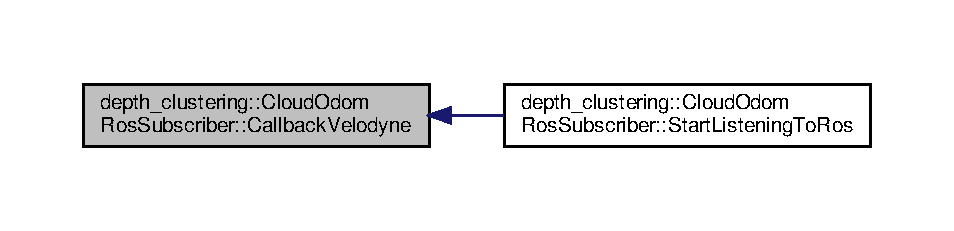
\includegraphics[width=350pt]{classdepth__clustering_1_1CloudOdomRosSubscriber_a8de806bc0b847229dcc92c504908f019_icgraph}
\end{center}
\end{figure}


The documentation for this class was generated from the following files\+:\begin{DoxyCompactItemize}
\item 
/home/ashwin/catkin\+\_\+ws/src/depth\+\_\+clustering/src/ros\+\_\+bridge/cloud\+\_\+odom\+\_\+ros\+\_\+subscriber.\+h\item 
/home/ashwin/catkin\+\_\+ws/src/depth\+\_\+clustering/src/ros\+\_\+bridge/cloud\+\_\+odom\+\_\+ros\+\_\+subscriber.\+cpp\end{DoxyCompactItemize}

\hypertarget{classdepth__clustering_1_1CloudProjection}{}\section{depth\+\_\+clustering\+:\+:Cloud\+Projection Class Reference}
\label{classdepth__clustering_1_1CloudProjection}\index{depth\+\_\+clustering\+::\+Cloud\+Projection@{depth\+\_\+clustering\+::\+Cloud\+Projection}}


Abstract class for cloud projection.  




{\ttfamily \#include $<$cloud\+\_\+projection.\+h$>$}

\subsection*{Classes}
\begin{DoxyCompactItemize}
\item 
class \hyperlink{classdepth__clustering_1_1CloudProjection_1_1PointContainer}{Point\+Container}
\begin{DoxyCompactList}\small\item\em Class for point container. \end{DoxyCompactList}\end{DoxyCompactItemize}
\subsection*{Public Types}
\begin{DoxyCompactItemize}
\item 
\mbox{\Hypertarget{classdepth__clustering_1_1CloudProjection_a691e153edbc93d274edfb35683cb17a0}\label{classdepth__clustering_1_1CloudProjection_a691e153edbc93d274edfb35683cb17a0}} 
enum {\bfseries Type} \{ {\bfseries S\+P\+H\+E\+R\+I\+C\+AL}, 
{\bfseries C\+Y\+L\+L\+I\+N\+D\+R\+I\+C\+AL}
 \}
\item 
\mbox{\Hypertarget{classdepth__clustering_1_1CloudProjection_a7ac49f27b97e149be239a777587b4162}\label{classdepth__clustering_1_1CloudProjection_a7ac49f27b97e149be239a777587b4162}} 
using {\bfseries Ptr} = shared\+\_\+ptr$<$ \hyperlink{classdepth__clustering_1_1CloudProjection}{Cloud\+Projection} $>$
\item 
\mbox{\Hypertarget{classdepth__clustering_1_1CloudProjection_aa7a2a7f37a6ebd5533e336e1f484567a}\label{classdepth__clustering_1_1CloudProjection_aa7a2a7f37a6ebd5533e336e1f484567a}} 
using {\bfseries Const\+Ptr} = shared\+\_\+ptr$<$ const \hyperlink{classdepth__clustering_1_1CloudProjection}{Cloud\+Projection} $>$
\end{DoxyCompactItemize}
\subsection*{Public Member Functions}
\begin{DoxyCompactItemize}
\item 
\mbox{\Hypertarget{classdepth__clustering_1_1CloudProjection_a7abfd6e56bacd684379916af2ab60cef}\label{classdepth__clustering_1_1CloudProjection_a7abfd6e56bacd684379916af2ab60cef}} 
{\bfseries Cloud\+Projection} (const \hyperlink{classdepth__clustering_1_1ProjectionParams}{Projection\+Params} \&params)
\item 
virtual void \hyperlink{classdepth__clustering_1_1CloudProjection_aab5fa3b7362b2c4297bf9b445ccc7ff8}{Init\+From\+Points} (const Rich\+Point\+::\+Aligned\+Vector \&points)=0
\begin{DoxyCompactList}\small\item\em Initialize from 3d points. \end{DoxyCompactList}\item 
virtual Cloud\+Projection\+::\+Ptr \hyperlink{classdepth__clustering_1_1CloudProjection_ae06ff9699c1a37c535b39fa6f722fa2e}{Clone} () const =0
\begin{DoxyCompactList}\small\item\em Polymorphic clone of a projection. \end{DoxyCompactList}\item 
\mbox{\Hypertarget{classdepth__clustering_1_1CloudProjection_ad1d88848db02e2d7e81e8c0e20407db5}\label{classdepth__clustering_1_1CloudProjection_ad1d88848db02e2d7e81e8c0e20407db5}} 
const cv\+::\+Mat \& {\bfseries depth\+\_\+image} () const
\item 
\mbox{\Hypertarget{classdepth__clustering_1_1CloudProjection_aa04e09c527c7e1bc1b5ab161c5931b30}\label{classdepth__clustering_1_1CloudProjection_aa04e09c527c7e1bc1b5ab161c5931b30}} 
cv\+::\+Mat \& {\bfseries depth\+\_\+image} ()
\item 
\mbox{\Hypertarget{classdepth__clustering_1_1CloudProjection_a3e28dfda41fa497bfd54fe3c7f2a9b37}\label{classdepth__clustering_1_1CloudProjection_a3e28dfda41fa497bfd54fe3c7f2a9b37}} 
void {\bfseries Clone\+Depth\+Image} (const cv\+::\+Mat \&image)
\item 
\mbox{\Hypertarget{classdepth__clustering_1_1CloudProjection_a7fb447ce48a63904a758ce6eef2fc8a1}\label{classdepth__clustering_1_1CloudProjection_a7fb447ce48a63904a758ce6eef2fc8a1}} 
size\+\_\+t {\bfseries rows} () const
\item 
\mbox{\Hypertarget{classdepth__clustering_1_1CloudProjection_a6f5be6a4cd14c458a0eb020d9573d17c}\label{classdepth__clustering_1_1CloudProjection_a6f5be6a4cd14c458a0eb020d9573d17c}} 
size\+\_\+t {\bfseries cols} () const
\item 
\mbox{\Hypertarget{classdepth__clustering_1_1CloudProjection_a2973d1a5e364ecbd2ae8838dbccfc59b}\label{classdepth__clustering_1_1CloudProjection_a2973d1a5e364ecbd2ae8838dbccfc59b}} 
size\+\_\+t {\bfseries size} () const
\item 
\mbox{\Hypertarget{classdepth__clustering_1_1CloudProjection_a6afd8a8c752e19705c62d96b35ae61d0}\label{classdepth__clustering_1_1CloudProjection_a6afd8a8c752e19705c62d96b35ae61d0}} 
const \hyperlink{classdepth__clustering_1_1ProjectionParams}{Projection\+Params} \& {\bfseries params} () const
\item 
\mbox{\Hypertarget{classdepth__clustering_1_1CloudProjection_ad452c4ae44f413d19a6bbb0210483152}\label{classdepth__clustering_1_1CloudProjection_ad452c4ae44f413d19a6bbb0210483152}} 
const \hyperlink{classdepth__clustering_1_1CloudProjection_1_1PointContainer}{Point\+Container} \& {\bfseries at} (const size\+\_\+t row, const size\+\_\+t col) const
\item 
\mbox{\Hypertarget{classdepth__clustering_1_1CloudProjection_a72001e572391d9fba69f2572ac6369f5}\label{classdepth__clustering_1_1CloudProjection_a72001e572391d9fba69f2572ac6369f5}} 
\hyperlink{classdepth__clustering_1_1CloudProjection_1_1PointContainer}{Point\+Container} \& {\bfseries at} (const size\+\_\+t row, const size\+\_\+t col)
\item 
\mbox{\Hypertarget{classdepth__clustering_1_1CloudProjection_a3806044cabf6286a5b66f1a3b295009f}\label{classdepth__clustering_1_1CloudProjection_a3806044cabf6286a5b66f1a3b295009f}} 
const Point\+Matrix \& {\bfseries matrix} () const
\item 
void \hyperlink{classdepth__clustering_1_1CloudProjection_ad92d5819092ef3e4aabd4da3a5775f38}{Check\+Image\+And\+Storage} (const cv\+::\+Mat \&image)
\begin{DoxyCompactList}\small\item\em Check if where we store data is valid. \end{DoxyCompactList}\item 
void \hyperlink{classdepth__clustering_1_1CloudProjection_a3bd71fd09ce42208b793d763637a527b}{Check\+Cloud\+And\+Storage} (const Rich\+Point\+::\+Aligned\+Vector \&points)
\begin{DoxyCompactList}\small\item\em Check if where we store data is valid. \end{DoxyCompactList}\item 
virtual \hyperlink{classdepth__clustering_1_1RichPoint}{Rich\+Point} \hyperlink{classdepth__clustering_1_1CloudProjection_ab552ac1dbb56e077679d9f0268c79a44}{Unproject\+Point} (const cv\+::\+Mat \&image, const int row, const int col) const
\begin{DoxyCompactList}\small\item\em Unproject a point from depth image coordinate. \end{DoxyCompactList}\item 
void \hyperlink{classdepth__clustering_1_1CloudProjection_afcc642064042bba2a1112ed2a37190f9}{Set\+Corrections} (const std\+::vector$<$ float $>$ \&corrections)
\begin{DoxyCompactList}\small\item\em Set corrections for systematic error in a dataset (see notebooks in the repo) \end{DoxyCompactList}\item 
\mbox{\Hypertarget{classdepth__clustering_1_1CloudProjection_a84476c5e25ccf70876f67622a280ac63}\label{classdepth__clustering_1_1CloudProjection_a84476c5e25ccf70876f67622a280ac63}} 
void \hyperlink{classdepth__clustering_1_1CloudProjection_a84476c5e25ccf70876f67622a280ac63}{Fix\+Depth\+Systematic\+Error\+If\+Needed} ()
\begin{DoxyCompactList}\small\item\em Fix systematic error. See notebooks in the repo for details. \end{DoxyCompactList}\end{DoxyCompactItemize}
\subsection*{Protected Attributes}
\begin{DoxyCompactItemize}
\item 
\mbox{\Hypertarget{classdepth__clustering_1_1CloudProjection_a3f70579b10bd93a7d5ac4b1f0d387701}\label{classdepth__clustering_1_1CloudProjection_a3f70579b10bd93a7d5ac4b1f0d387701}} 
Point\+Matrix {\bfseries \+\_\+data}
\item 
\mbox{\Hypertarget{classdepth__clustering_1_1CloudProjection_a8978a85d52212a2a88cbb3c6791eddd6}\label{classdepth__clustering_1_1CloudProjection_a8978a85d52212a2a88cbb3c6791eddd6}} 
\hyperlink{classdepth__clustering_1_1ProjectionParams}{Projection\+Params} {\bfseries \+\_\+params}
\item 
\mbox{\Hypertarget{classdepth__clustering_1_1CloudProjection_a2d239a9a0fcaada00de36aad436e2af2}\label{classdepth__clustering_1_1CloudProjection_a2d239a9a0fcaada00de36aad436e2af2}} 
cv\+::\+Mat {\bfseries \+\_\+depth\+\_\+image}
\item 
\mbox{\Hypertarget{classdepth__clustering_1_1CloudProjection_a034b1066d16e2215016ab11f6c323aef}\label{classdepth__clustering_1_1CloudProjection_a034b1066d16e2215016ab11f6c323aef}} 
std\+::vector$<$ float $>$ {\bfseries \+\_\+corrections}
\end{DoxyCompactItemize}


\subsection{Detailed Description}
Abstract class for cloud projection. 

Inheritance diagram for depth\+\_\+clustering\+:\+:Cloud\+Projection\+:\nopagebreak
\begin{figure}[H]
\begin{center}
\leavevmode
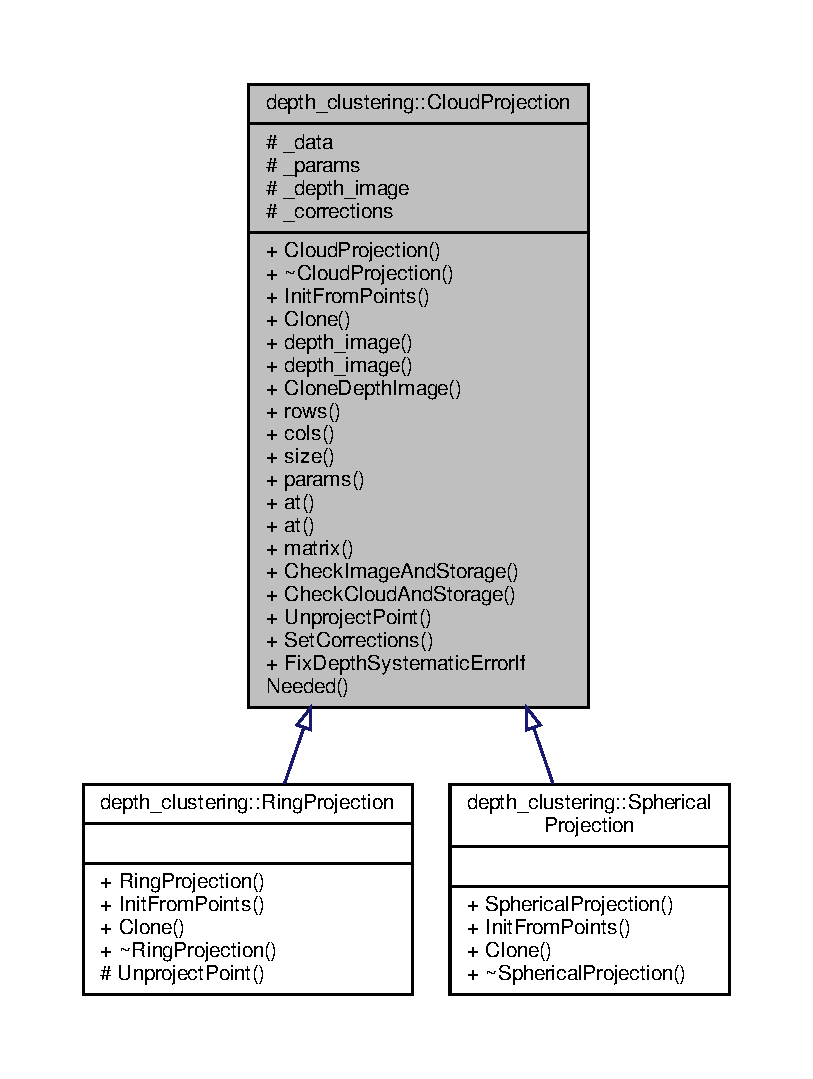
\includegraphics[width=350pt]{classdepth__clustering_1_1CloudProjection__inherit__graph}
\end{center}
\end{figure}


Collaboration diagram for depth\+\_\+clustering\+:\+:Cloud\+Projection\+:\nopagebreak
\begin{figure}[H]
\begin{center}
\leavevmode
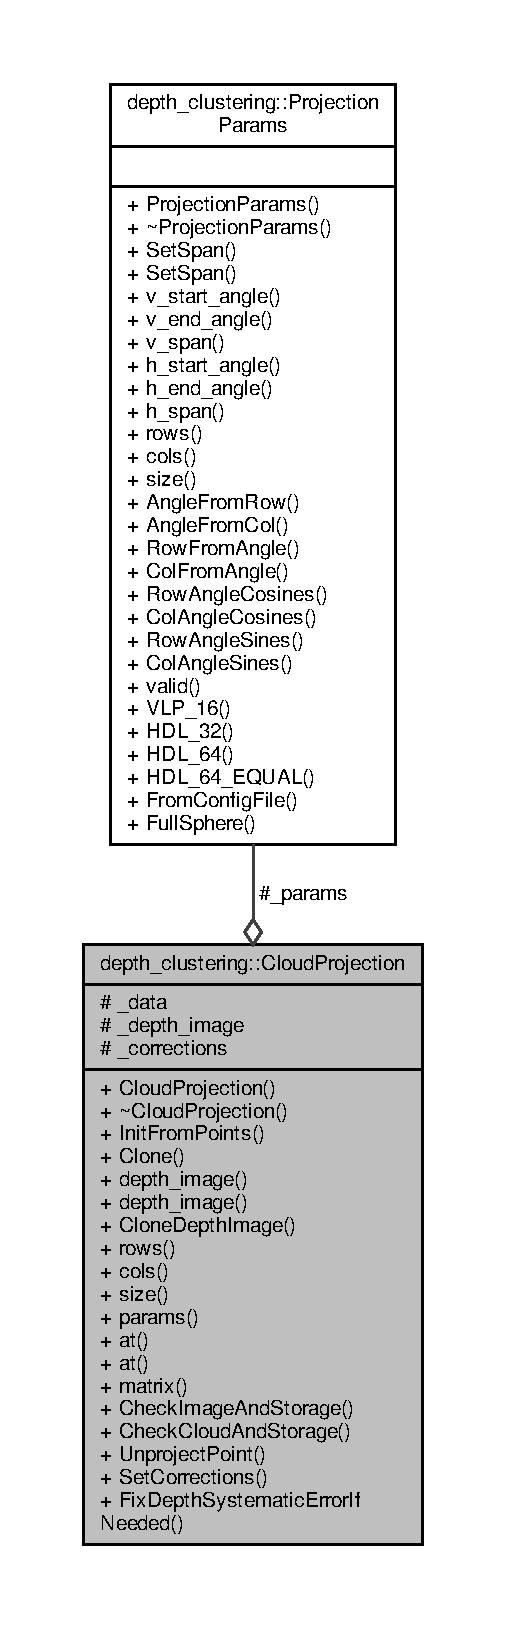
\includegraphics[height=550pt]{classdepth__clustering_1_1CloudProjection__coll__graph}
\end{center}
\end{figure}


\subsection{Member Function Documentation}
\mbox{\Hypertarget{classdepth__clustering_1_1CloudProjection_a3bd71fd09ce42208b793d763637a527b}\label{classdepth__clustering_1_1CloudProjection_a3bd71fd09ce42208b793d763637a527b}} 
\index{depth\+\_\+clustering\+::\+Cloud\+Projection@{depth\+\_\+clustering\+::\+Cloud\+Projection}!Check\+Cloud\+And\+Storage@{Check\+Cloud\+And\+Storage}}
\index{Check\+Cloud\+And\+Storage@{Check\+Cloud\+And\+Storage}!depth\+\_\+clustering\+::\+Cloud\+Projection@{depth\+\_\+clustering\+::\+Cloud\+Projection}}
\subsubsection{\texorpdfstring{Check\+Cloud\+And\+Storage()}{CheckCloudAndStorage()}}
{\footnotesize\ttfamily void depth\+\_\+clustering\+::\+Cloud\+Projection\+::\+Check\+Cloud\+And\+Storage (\begin{DoxyParamCaption}\item[{const Rich\+Point\+::\+Aligned\+Vector \&}]{points }\end{DoxyParamCaption})}



Check if where we store data is valid. 


\begin{DoxyParams}[1]{Parameters}
\mbox{\tt in}  & {\em points} & The points to check \\
\hline
\end{DoxyParams}
Here is the caller graph for this function\+:\nopagebreak
\begin{figure}[H]
\begin{center}
\leavevmode
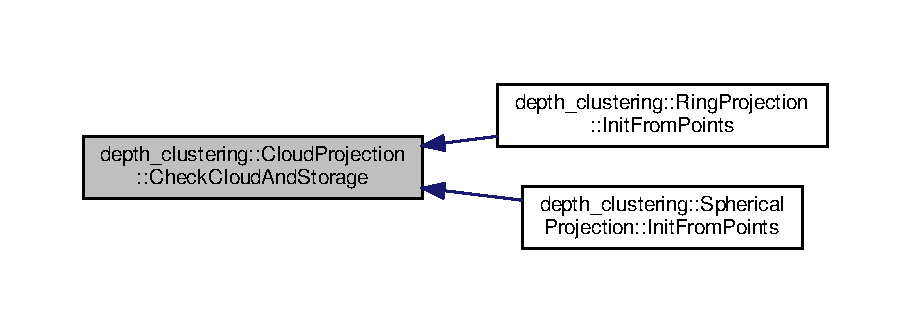
\includegraphics[width=350pt]{classdepth__clustering_1_1CloudProjection_a3bd71fd09ce42208b793d763637a527b_icgraph}
\end{center}
\end{figure}
\mbox{\Hypertarget{classdepth__clustering_1_1CloudProjection_ad92d5819092ef3e4aabd4da3a5775f38}\label{classdepth__clustering_1_1CloudProjection_ad92d5819092ef3e4aabd4da3a5775f38}} 
\index{depth\+\_\+clustering\+::\+Cloud\+Projection@{depth\+\_\+clustering\+::\+Cloud\+Projection}!Check\+Image\+And\+Storage@{Check\+Image\+And\+Storage}}
\index{Check\+Image\+And\+Storage@{Check\+Image\+And\+Storage}!depth\+\_\+clustering\+::\+Cloud\+Projection@{depth\+\_\+clustering\+::\+Cloud\+Projection}}
\subsubsection{\texorpdfstring{Check\+Image\+And\+Storage()}{CheckImageAndStorage()}}
{\footnotesize\ttfamily void depth\+\_\+clustering\+::\+Cloud\+Projection\+::\+Check\+Image\+And\+Storage (\begin{DoxyParamCaption}\item[{const cv\+::\+Mat \&}]{image }\end{DoxyParamCaption})}



Check if where we store data is valid. 


\begin{DoxyParams}[1]{Parameters}
\mbox{\tt in}  & {\em image} & The image to check \\
\hline
\end{DoxyParams}
\mbox{\Hypertarget{classdepth__clustering_1_1CloudProjection_ae06ff9699c1a37c535b39fa6f722fa2e}\label{classdepth__clustering_1_1CloudProjection_ae06ff9699c1a37c535b39fa6f722fa2e}} 
\index{depth\+\_\+clustering\+::\+Cloud\+Projection@{depth\+\_\+clustering\+::\+Cloud\+Projection}!Clone@{Clone}}
\index{Clone@{Clone}!depth\+\_\+clustering\+::\+Cloud\+Projection@{depth\+\_\+clustering\+::\+Cloud\+Projection}}
\subsubsection{\texorpdfstring{Clone()}{Clone()}}
{\footnotesize\ttfamily virtual Cloud\+Projection\+::\+Ptr depth\+\_\+clustering\+::\+Cloud\+Projection\+::\+Clone (\begin{DoxyParamCaption}{ }\end{DoxyParamCaption}) const\hspace{0.3cm}{\ttfamily [pure virtual]}}



Polymorphic clone of a projection. 

\begin{DoxyReturn}{Returns}
Shared pointer of a copy of this object. 
\end{DoxyReturn}


Implemented in \hyperlink{classdepth__clustering_1_1RingProjection_a433c0ee114b89b6c78ad4c471d120153}{depth\+\_\+clustering\+::\+Ring\+Projection}, and \hyperlink{classdepth__clustering_1_1SphericalProjection_a1b7870502497310666b2909701906470}{depth\+\_\+clustering\+::\+Spherical\+Projection}.

\mbox{\Hypertarget{classdepth__clustering_1_1CloudProjection_aab5fa3b7362b2c4297bf9b445ccc7ff8}\label{classdepth__clustering_1_1CloudProjection_aab5fa3b7362b2c4297bf9b445ccc7ff8}} 
\index{depth\+\_\+clustering\+::\+Cloud\+Projection@{depth\+\_\+clustering\+::\+Cloud\+Projection}!Init\+From\+Points@{Init\+From\+Points}}
\index{Init\+From\+Points@{Init\+From\+Points}!depth\+\_\+clustering\+::\+Cloud\+Projection@{depth\+\_\+clustering\+::\+Cloud\+Projection}}
\subsubsection{\texorpdfstring{Init\+From\+Points()}{InitFromPoints()}}
{\footnotesize\ttfamily virtual void depth\+\_\+clustering\+::\+Cloud\+Projection\+::\+Init\+From\+Points (\begin{DoxyParamCaption}\item[{const Rich\+Point\+::\+Aligned\+Vector \&}]{points }\end{DoxyParamCaption})\hspace{0.3cm}{\ttfamily [pure virtual]}}



Initialize from 3d points. 


\begin{DoxyParams}[1]{Parameters}
\mbox{\tt in}  & {\em points} & The points \\
\hline
\end{DoxyParams}


Implemented in \hyperlink{classdepth__clustering_1_1RingProjection_acfda4cfe9a0b80936987691fe44fc79c}{depth\+\_\+clustering\+::\+Ring\+Projection}, and \hyperlink{classdepth__clustering_1_1SphericalProjection_ab80cb1d72f60e7a887affa0ab10ebc03}{depth\+\_\+clustering\+::\+Spherical\+Projection}.

\mbox{\Hypertarget{classdepth__clustering_1_1CloudProjection_afcc642064042bba2a1112ed2a37190f9}\label{classdepth__clustering_1_1CloudProjection_afcc642064042bba2a1112ed2a37190f9}} 
\index{depth\+\_\+clustering\+::\+Cloud\+Projection@{depth\+\_\+clustering\+::\+Cloud\+Projection}!Set\+Corrections@{Set\+Corrections}}
\index{Set\+Corrections@{Set\+Corrections}!depth\+\_\+clustering\+::\+Cloud\+Projection@{depth\+\_\+clustering\+::\+Cloud\+Projection}}
\subsubsection{\texorpdfstring{Set\+Corrections()}{SetCorrections()}}
{\footnotesize\ttfamily void depth\+\_\+clustering\+::\+Cloud\+Projection\+::\+Set\+Corrections (\begin{DoxyParamCaption}\item[{const std\+::vector$<$ float $>$ \&}]{corrections }\end{DoxyParamCaption})\hspace{0.3cm}{\ttfamily [inline]}}



Set corrections for systematic error in a dataset (see notebooks in the repo) 


\begin{DoxyParams}[1]{Parameters}
\mbox{\tt in}  & {\em corrections} & A vector of correction in depth for every beam. \\
\hline
\end{DoxyParams}
Here is the call graph for this function\+:\nopagebreak
\begin{figure}[H]
\begin{center}
\leavevmode
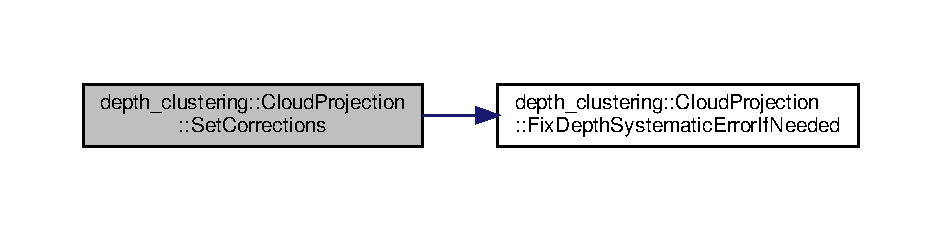
\includegraphics[width=350pt]{classdepth__clustering_1_1CloudProjection_afcc642064042bba2a1112ed2a37190f9_cgraph}
\end{center}
\end{figure}
\mbox{\Hypertarget{classdepth__clustering_1_1CloudProjection_ab552ac1dbb56e077679d9f0268c79a44}\label{classdepth__clustering_1_1CloudProjection_ab552ac1dbb56e077679d9f0268c79a44}} 
\index{depth\+\_\+clustering\+::\+Cloud\+Projection@{depth\+\_\+clustering\+::\+Cloud\+Projection}!Unproject\+Point@{Unproject\+Point}}
\index{Unproject\+Point@{Unproject\+Point}!depth\+\_\+clustering\+::\+Cloud\+Projection@{depth\+\_\+clustering\+::\+Cloud\+Projection}}
\subsubsection{\texorpdfstring{Unproject\+Point()}{UnprojectPoint()}}
{\footnotesize\ttfamily \hyperlink{classdepth__clustering_1_1RichPoint}{Rich\+Point} depth\+\_\+clustering\+::\+Cloud\+Projection\+::\+Unproject\+Point (\begin{DoxyParamCaption}\item[{const cv\+::\+Mat \&}]{image,  }\item[{const int}]{row,  }\item[{const int}]{col }\end{DoxyParamCaption}) const\hspace{0.3cm}{\ttfamily [virtual]}}



Unproject a point from depth image coordinate. 


\begin{DoxyParams}[1]{Parameters}
\mbox{\tt in}  & {\em image} & A depth image \\
\hline
\mbox{\tt in}  & {\em row} & A row in the image \\
\hline
\mbox{\tt in}  & {\em col} & A col in the image\\
\hline
\end{DoxyParams}
\begin{DoxyReturn}{Returns}
\{ description\+\_\+of\+\_\+the\+\_\+return\+\_\+value \} 
\end{DoxyReturn}


Reimplemented in \hyperlink{classdepth__clustering_1_1RingProjection_a16cbf43e541e65560cb282c560b4efa7}{depth\+\_\+clustering\+::\+Ring\+Projection}.

Here is the caller graph for this function\+:\nopagebreak
\begin{figure}[H]
\begin{center}
\leavevmode
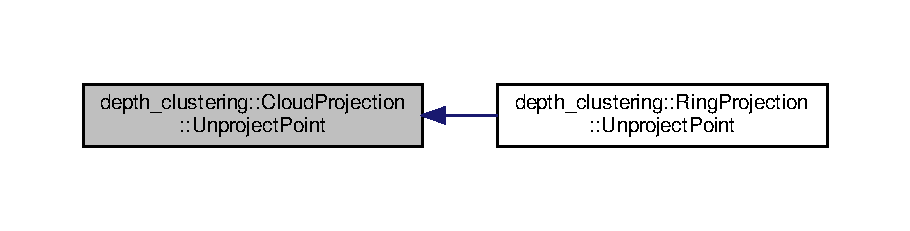
\includegraphics[width=350pt]{classdepth__clustering_1_1CloudProjection_ab552ac1dbb56e077679d9f0268c79a44_icgraph}
\end{center}
\end{figure}


The documentation for this class was generated from the following files\+:\begin{DoxyCompactItemize}
\item 
/home/ashwin/catkin\+\_\+ws/src/depth\+\_\+clustering/src/projections/cloud\+\_\+projection.\+h\item 
/home/ashwin/catkin\+\_\+ws/src/depth\+\_\+clustering/src/projections/cloud\+\_\+projection.\+cpp\end{DoxyCompactItemize}

\hypertarget{classdepth__clustering_1_1DepthGroundRemover}{}\section{depth\+\_\+clustering\+:\+:Depth\+Ground\+Remover Class Reference}
\label{classdepth__clustering_1_1DepthGroundRemover}\index{depth\+\_\+clustering\+::\+Depth\+Ground\+Remover@{depth\+\_\+clustering\+::\+Depth\+Ground\+Remover}}


A class to remove ground based upon depth image.  




{\ttfamily \#include $<$depth\+\_\+ground\+\_\+remover.\+h$>$}

\subsection*{Public Member Functions}
\begin{DoxyCompactItemize}
\item 
\mbox{\Hypertarget{classdepth__clustering_1_1DepthGroundRemover_aae9816017a747246c495de41bcece02c}\label{classdepth__clustering_1_1DepthGroundRemover_aae9816017a747246c495de41bcece02c}} 
{\bfseries Depth\+Ground\+Remover} (const \hyperlink{classdepth__clustering_1_1ProjectionParams}{Projection\+Params} \&params, const Radians \&ground\+\_\+remove\+\_\+angle, int window\+\_\+size=5)
\item 
void \hyperlink{classdepth__clustering_1_1DepthGroundRemover_ab2c3bcc8df6cc70ad5057f5ec3bd074f}{On\+New\+Object\+Received} (const \hyperlink{classdepth__clustering_1_1Cloud}{Cloud} \&cloud, const int sender\+\_\+id) override
\begin{DoxyCompactList}\small\item\em when someone sends us an object we process it \end{DoxyCompactList}\end{DoxyCompactItemize}
\subsection*{Protected Member Functions}
\begin{DoxyCompactItemize}
\item 
cv\+::\+Mat \hyperlink{classdepth__clustering_1_1DepthGroundRemover_a81aa3a52c70223555b4f4e1800e05022}{Zero\+Out\+Ground} (const cv\+::\+Mat \&image, const cv\+::\+Mat \&angle\+\_\+image, const Radians \&threshold) const
\begin{DoxyCompactList}\small\item\em Zero out all pixels that belong to ground. \end{DoxyCompactList}\item 
\mbox{\Hypertarget{classdepth__clustering_1_1DepthGroundRemover_a00ce5997c0dd1692c35ff0a28b94b1b1}\label{classdepth__clustering_1_1DepthGroundRemover_a00ce5997c0dd1692c35ff0a28b94b1b1}} 
cv\+::\+Mat {\bfseries Zero\+Out\+Ground\+B\+FS} (const cv\+::\+Mat \&image, const cv\+::\+Mat \&angle\+\_\+image, const Radians \&threshold, int kernel\+\_\+size) const
\item 
cv\+::\+Mat \hyperlink{classdepth__clustering_1_1DepthGroundRemover_af533c51a44aad9a56c12445b61b801b9}{Create\+Angle\+Image} (const cv\+::\+Mat \&depth\+\_\+image)
\begin{DoxyCompactList}\small\item\em create a help image with angle in radians written for each pixel \end{DoxyCompactList}\item 
cv\+::\+Mat \hyperlink{classdepth__clustering_1_1DepthGroundRemover_a2aeaac524f19861b26c171d845f67e2e}{Get\+Savitsky\+Golay\+Kernel} (int window\+\_\+size) const
\begin{DoxyCompactList}\small\item\em Get kernel for Savitsky-\/\+Golay filter. \end{DoxyCompactList}\item 
\mbox{\Hypertarget{classdepth__clustering_1_1DepthGroundRemover_a7d67b35fdeaa5fc093cbd857b1405481}\label{classdepth__clustering_1_1DepthGroundRemover_a7d67b35fdeaa5fc093cbd857b1405481}} 
cv\+::\+Mat {\bfseries Get\+Uniform\+Kernel} (int window\+\_\+size, int \hyperlink{classdepth__clustering_1_1AbstractSender_a6120bda97c12587db40f34ed73b45475}{type}=C\+V\+\_\+32F) const
\item 
cv\+::\+Mat \hyperlink{classdepth__clustering_1_1DepthGroundRemover_a63b32fa801a13021bf22699525579f8b}{Apply\+Savitsky\+Golay\+Smoothing} (const cv\+::\+Mat \&column, int window\+\_\+size)
\begin{DoxyCompactList}\small\item\em Apply Savitsky-\/\+Golay smoothing to a column. \end{DoxyCompactList}\item 
Radians \hyperlink{classdepth__clustering_1_1DepthGroundRemover_a29ba07a101794aab322ae3c0671806e0}{Get\+Line\+Angle} (const cv\+::\+Mat \&depth\+\_\+image, int col, int row\+\_\+curr, int row\+\_\+neigh)
\begin{DoxyCompactList}\small\item\em Get line angle. \end{DoxyCompactList}\item 
cv\+::\+Mat \hyperlink{classdepth__clustering_1_1DepthGroundRemover_a51dd313ed1bdda2188fb3a3fa1c5738e}{Repair\+Depth} (const cv\+::\+Mat \&no\+\_\+ground\+\_\+image, int step, float depth\+\_\+threshold)
\begin{DoxyCompactList}\small\item\em Repair zeros in the depth image. \end{DoxyCompactList}\item 
\mbox{\Hypertarget{classdepth__clustering_1_1DepthGroundRemover_ab44815e8ea8b10abce24faebf8322624}\label{classdepth__clustering_1_1DepthGroundRemover_ab44815e8ea8b10abce24faebf8322624}} 
cv\+::\+Mat {\bfseries Repair\+Depth} (const cv\+::\+Mat \&depth\+\_\+image)
\end{DoxyCompactItemize}
\subsection*{Protected Attributes}
\begin{DoxyCompactItemize}
\item 
\mbox{\Hypertarget{classdepth__clustering_1_1DepthGroundRemover_ad4ff83331f7ad6a3bbb22ce5356471ed}\label{classdepth__clustering_1_1DepthGroundRemover_ad4ff83331f7ad6a3bbb22ce5356471ed}} 
\hyperlink{classdepth__clustering_1_1ProjectionParams}{Projection\+Params} {\bfseries \+\_\+params}
\item 
\mbox{\Hypertarget{classdepth__clustering_1_1DepthGroundRemover_a44a1a7778c4913540c9fd3545671ee96}\label{classdepth__clustering_1_1DepthGroundRemover_a44a1a7778c4913540c9fd3545671ee96}} 
int {\bfseries \+\_\+window\+\_\+size} = 5
\item 
\mbox{\Hypertarget{classdepth__clustering_1_1DepthGroundRemover_a6acd966842064c50552cfd3857652cd8}\label{classdepth__clustering_1_1DepthGroundRemover_a6acd966842064c50552cfd3857652cd8}} 
Radians {\bfseries \+\_\+ground\+\_\+remove\+\_\+angle} = 5\+\_\+deg
\item 
\mbox{\Hypertarget{classdepth__clustering_1_1DepthGroundRemover_a1d27a305647b5315b1c2a46c4b0a3039}\label{classdepth__clustering_1_1DepthGroundRemover_a1d27a305647b5315b1c2a46c4b0a3039}} 
float {\bfseries \+\_\+eps} = 0.\+001f
\item 
\mbox{\Hypertarget{classdepth__clustering_1_1DepthGroundRemover_a5230ebdee643d0e76c86486adf70db5d}\label{classdepth__clustering_1_1DepthGroundRemover_a5230ebdee643d0e76c86486adf70db5d}} 
int {\bfseries \+\_\+counter} = 0
\end{DoxyCompactItemize}
\subsection*{Additional Inherited Members}


\subsection{Detailed Description}
A class to remove ground based upon depth image. 

Given a depth image and image config this class should remove the ground and send the new depth image with no ground further through the pipeline to its clients.


\begin{DoxyParams}{Parameters}
{\em params} & projection params \\
\hline
\end{DoxyParams}


Inheritance diagram for depth\+\_\+clustering\+:\+:Depth\+Ground\+Remover\+:\nopagebreak
\begin{figure}[H]
\begin{center}
\leavevmode
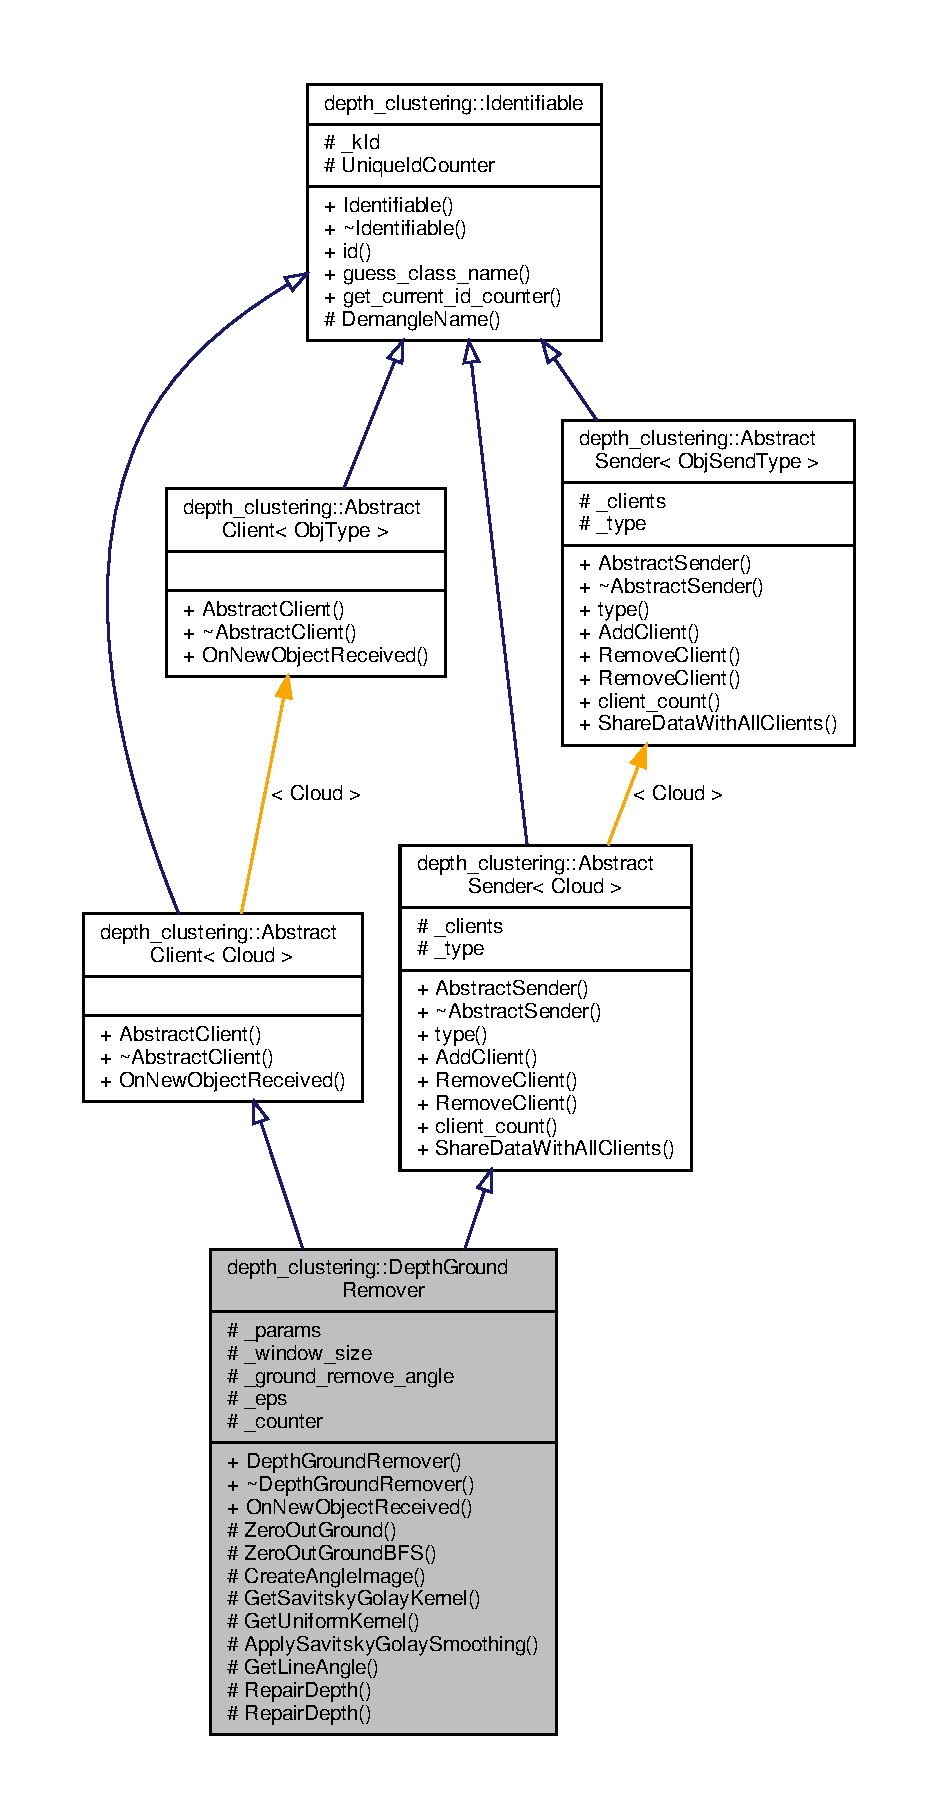
\includegraphics[height=550pt]{classdepth__clustering_1_1DepthGroundRemover__inherit__graph}
\end{center}
\end{figure}


Collaboration diagram for depth\+\_\+clustering\+:\+:Depth\+Ground\+Remover\+:\nopagebreak
\begin{figure}[H]
\begin{center}
\leavevmode
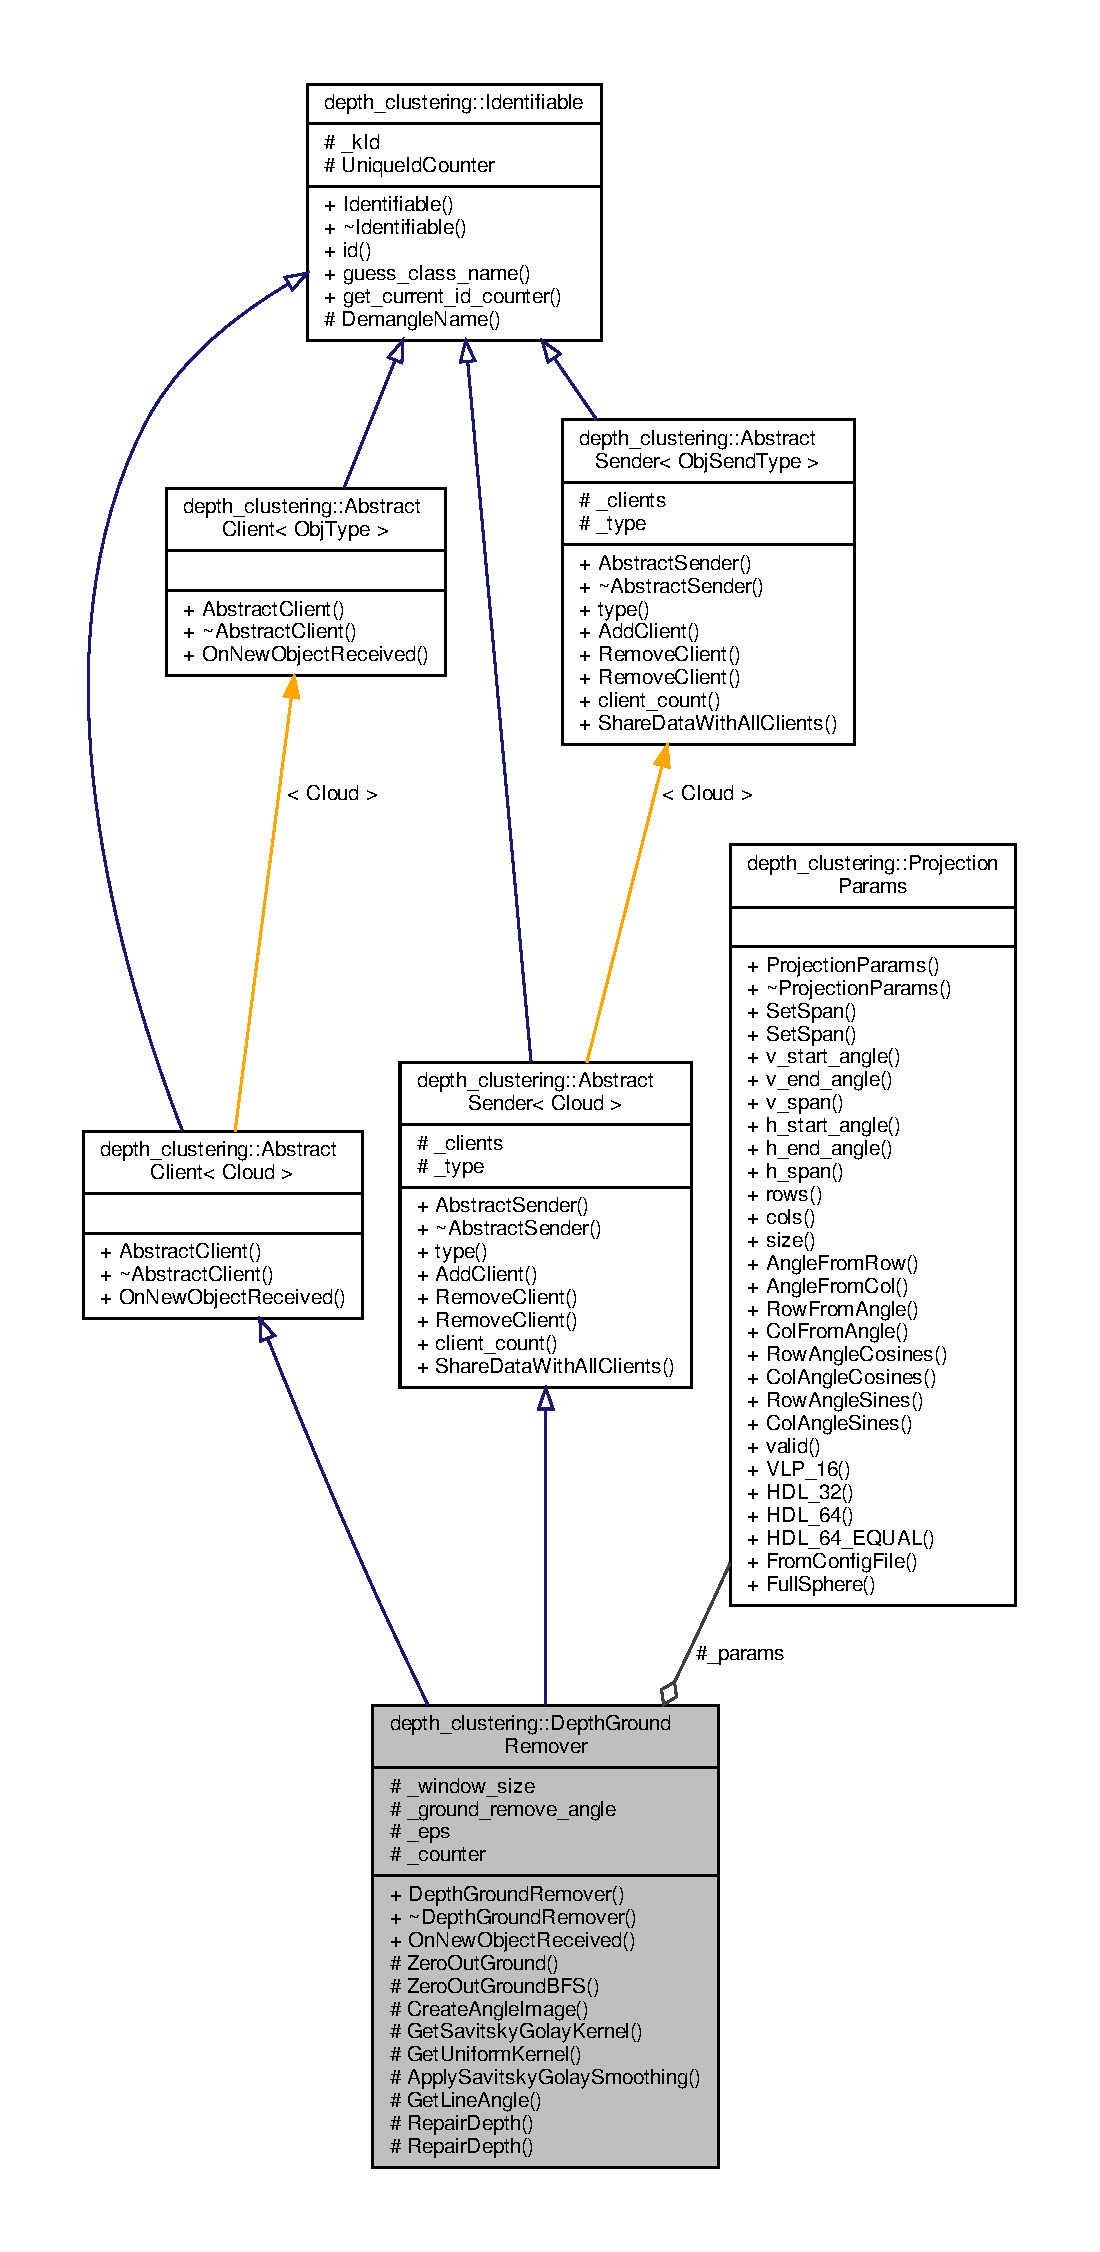
\includegraphics[height=550pt]{classdepth__clustering_1_1DepthGroundRemover__coll__graph}
\end{center}
\end{figure}


\subsection{Member Function Documentation}
\mbox{\Hypertarget{classdepth__clustering_1_1DepthGroundRemover_a63b32fa801a13021bf22699525579f8b}\label{classdepth__clustering_1_1DepthGroundRemover_a63b32fa801a13021bf22699525579f8b}} 
\index{depth\+\_\+clustering\+::\+Depth\+Ground\+Remover@{depth\+\_\+clustering\+::\+Depth\+Ground\+Remover}!Apply\+Savitsky\+Golay\+Smoothing@{Apply\+Savitsky\+Golay\+Smoothing}}
\index{Apply\+Savitsky\+Golay\+Smoothing@{Apply\+Savitsky\+Golay\+Smoothing}!depth\+\_\+clustering\+::\+Depth\+Ground\+Remover@{depth\+\_\+clustering\+::\+Depth\+Ground\+Remover}}
\subsubsection{\texorpdfstring{Apply\+Savitsky\+Golay\+Smoothing()}{ApplySavitskyGolaySmoothing()}}
{\footnotesize\ttfamily Mat depth\+\_\+clustering\+::\+Depth\+Ground\+Remover\+::\+Apply\+Savitsky\+Golay\+Smoothing (\begin{DoxyParamCaption}\item[{const cv\+::\+Mat \&}]{column,  }\item[{int}]{window\+\_\+size }\end{DoxyParamCaption})\hspace{0.3cm}{\ttfamily [protected]}}



Apply Savitsky-\/\+Golay smoothing to a column. 


\begin{DoxyParams}{Parameters}
{\em column} & \mbox{[}A column of an angle image\mbox{]} \\
\hline
\end{DoxyParams}
\begin{DoxyReturn}{Returns}
\mbox{[}a smoothed column\mbox{]} 
\end{DoxyReturn}
Here is the call graph for this function\+:\nopagebreak
\begin{figure}[H]
\begin{center}
\leavevmode
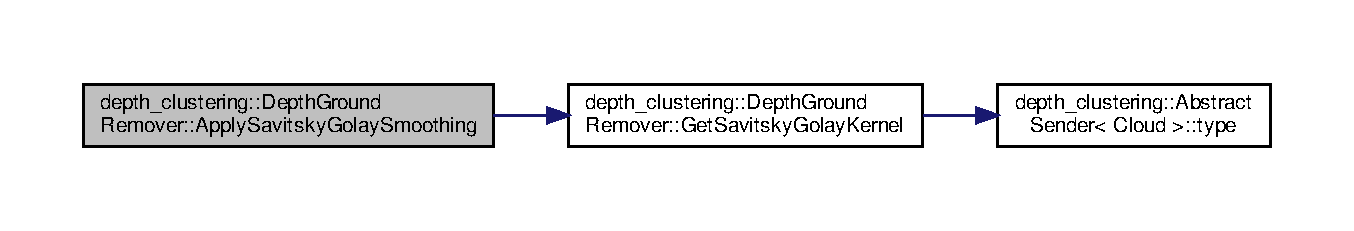
\includegraphics[width=350pt]{classdepth__clustering_1_1DepthGroundRemover_a63b32fa801a13021bf22699525579f8b_cgraph}
\end{center}
\end{figure}
Here is the caller graph for this function\+:\nopagebreak
\begin{figure}[H]
\begin{center}
\leavevmode
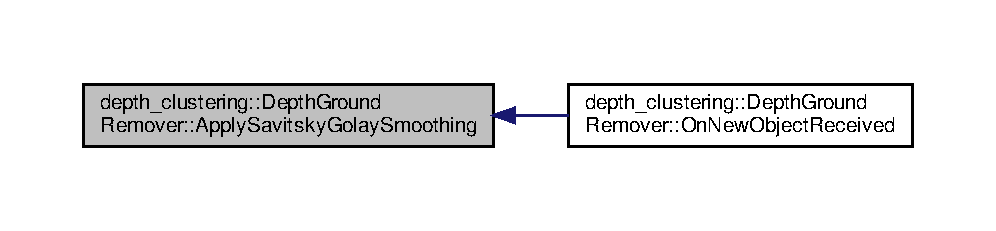
\includegraphics[width=350pt]{classdepth__clustering_1_1DepthGroundRemover_a63b32fa801a13021bf22699525579f8b_icgraph}
\end{center}
\end{figure}
\mbox{\Hypertarget{classdepth__clustering_1_1DepthGroundRemover_af533c51a44aad9a56c12445b61b801b9}\label{classdepth__clustering_1_1DepthGroundRemover_af533c51a44aad9a56c12445b61b801b9}} 
\index{depth\+\_\+clustering\+::\+Depth\+Ground\+Remover@{depth\+\_\+clustering\+::\+Depth\+Ground\+Remover}!Create\+Angle\+Image@{Create\+Angle\+Image}}
\index{Create\+Angle\+Image@{Create\+Angle\+Image}!depth\+\_\+clustering\+::\+Depth\+Ground\+Remover@{depth\+\_\+clustering\+::\+Depth\+Ground\+Remover}}
\subsubsection{\texorpdfstring{Create\+Angle\+Image()}{CreateAngleImage()}}
{\footnotesize\ttfamily Mat depth\+\_\+clustering\+::\+Depth\+Ground\+Remover\+::\+Create\+Angle\+Image (\begin{DoxyParamCaption}\item[{const cv\+::\+Mat \&}]{depth\+\_\+image }\end{DoxyParamCaption})\hspace{0.3cm}{\ttfamily [protected]}}



create a help image with angle in radians written for each pixel 


\begin{DoxyParams}{Parameters}
{\em depth\+\_\+image} & \mbox{[}input depth image\mbox{]} \\
\hline
\end{DoxyParams}
\begin{DoxyReturn}{Returns}
\mbox{[}32 bit float image with angle in radians written in every pixel\mbox{]} 
\end{DoxyReturn}
Here is the caller graph for this function\+:\nopagebreak
\begin{figure}[H]
\begin{center}
\leavevmode
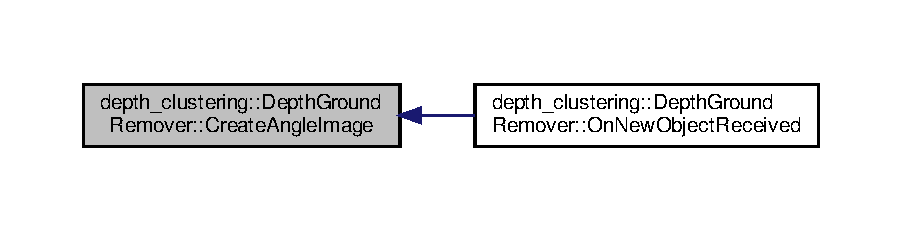
\includegraphics[width=350pt]{classdepth__clustering_1_1DepthGroundRemover_af533c51a44aad9a56c12445b61b801b9_icgraph}
\end{center}
\end{figure}
\mbox{\Hypertarget{classdepth__clustering_1_1DepthGroundRemover_a29ba07a101794aab322ae3c0671806e0}\label{classdepth__clustering_1_1DepthGroundRemover_a29ba07a101794aab322ae3c0671806e0}} 
\index{depth\+\_\+clustering\+::\+Depth\+Ground\+Remover@{depth\+\_\+clustering\+::\+Depth\+Ground\+Remover}!Get\+Line\+Angle@{Get\+Line\+Angle}}
\index{Get\+Line\+Angle@{Get\+Line\+Angle}!depth\+\_\+clustering\+::\+Depth\+Ground\+Remover@{depth\+\_\+clustering\+::\+Depth\+Ground\+Remover}}
\subsubsection{\texorpdfstring{Get\+Line\+Angle()}{GetLineAngle()}}
{\footnotesize\ttfamily Radians depth\+\_\+clustering\+::\+Depth\+Ground\+Remover\+::\+Get\+Line\+Angle (\begin{DoxyParamCaption}\item[{const cv\+::\+Mat \&}]{depth\+\_\+image,  }\item[{int}]{col,  }\item[{int}]{row\+\_\+curr,  }\item[{int}]{row\+\_\+neigh }\end{DoxyParamCaption})\hspace{0.3cm}{\ttfamily [protected]}}



Get line angle. 

Given two depth values and their angles compute the angle of the line that they spawn in the sensor frame.


\begin{DoxyParams}{Parameters}
{\em depth\+\_\+image} & \mbox{[}32 bit float image\mbox{]} \\
\hline
{\em col} & \mbox{[}current column\mbox{]} \\
\hline
{\em row\+\_\+curr} & \mbox{[}current row\mbox{]} \\
\hline
{\em row\+\_\+neigh} & \mbox{[}neighbor row\mbox{]} \\
\hline
\end{DoxyParams}
\begin{DoxyReturn}{Returns}
\mbox{[}angle of the line\mbox{]} 
\end{DoxyReturn}
Here is the call graph for this function\+:\nopagebreak
\begin{figure}[H]
\begin{center}
\leavevmode
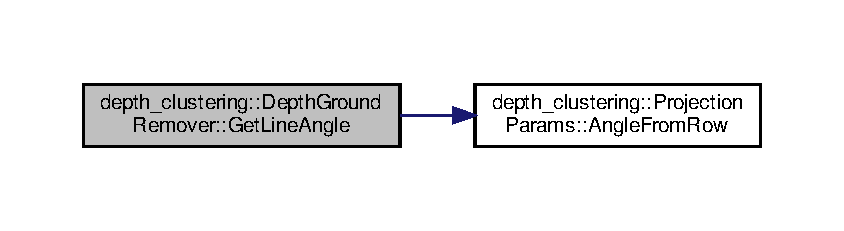
\includegraphics[width=350pt]{classdepth__clustering_1_1DepthGroundRemover_a29ba07a101794aab322ae3c0671806e0_cgraph}
\end{center}
\end{figure}
\mbox{\Hypertarget{classdepth__clustering_1_1DepthGroundRemover_a2aeaac524f19861b26c171d845f67e2e}\label{classdepth__clustering_1_1DepthGroundRemover_a2aeaac524f19861b26c171d845f67e2e}} 
\index{depth\+\_\+clustering\+::\+Depth\+Ground\+Remover@{depth\+\_\+clustering\+::\+Depth\+Ground\+Remover}!Get\+Savitsky\+Golay\+Kernel@{Get\+Savitsky\+Golay\+Kernel}}
\index{Get\+Savitsky\+Golay\+Kernel@{Get\+Savitsky\+Golay\+Kernel}!depth\+\_\+clustering\+::\+Depth\+Ground\+Remover@{depth\+\_\+clustering\+::\+Depth\+Ground\+Remover}}
\subsubsection{\texorpdfstring{Get\+Savitsky\+Golay\+Kernel()}{GetSavitskyGolayKernel()}}
{\footnotesize\ttfamily Mat depth\+\_\+clustering\+::\+Depth\+Ground\+Remover\+::\+Get\+Savitsky\+Golay\+Kernel (\begin{DoxyParamCaption}\item[{int}]{window\+\_\+size }\end{DoxyParamCaption}) const\hspace{0.3cm}{\ttfamily [protected]}}



Get kernel for Savitsky-\/\+Golay filter. 

Get a column filter to process an image filled with data with Savitsky-\/\+Golay filter


\begin{DoxyParams}{Parameters}
{\em window\+\_\+size} & size of the kernel \\
\hline
\end{DoxyParams}
\begin{DoxyReturn}{Returns}
column Mat kernel 
\end{DoxyReturn}
Here is the call graph for this function\+:\nopagebreak
\begin{figure}[H]
\begin{center}
\leavevmode
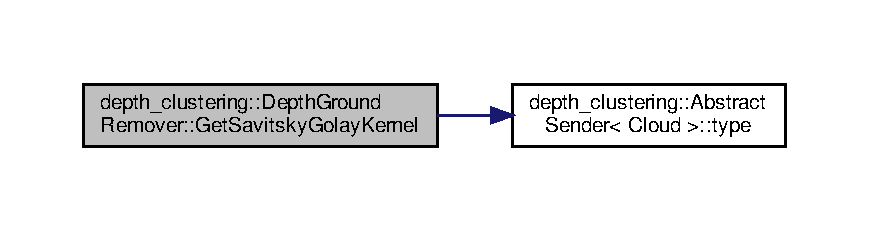
\includegraphics[width=350pt]{classdepth__clustering_1_1DepthGroundRemover_a2aeaac524f19861b26c171d845f67e2e_cgraph}
\end{center}
\end{figure}
Here is the caller graph for this function\+:\nopagebreak
\begin{figure}[H]
\begin{center}
\leavevmode
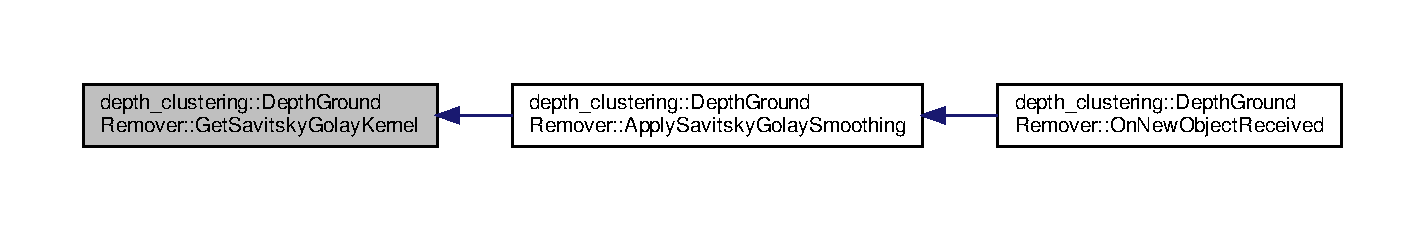
\includegraphics[width=350pt]{classdepth__clustering_1_1DepthGroundRemover_a2aeaac524f19861b26c171d845f67e2e_icgraph}
\end{center}
\end{figure}
\mbox{\Hypertarget{classdepth__clustering_1_1DepthGroundRemover_ab2c3bcc8df6cc70ad5057f5ec3bd074f}\label{classdepth__clustering_1_1DepthGroundRemover_ab2c3bcc8df6cc70ad5057f5ec3bd074f}} 
\index{depth\+\_\+clustering\+::\+Depth\+Ground\+Remover@{depth\+\_\+clustering\+::\+Depth\+Ground\+Remover}!On\+New\+Object\+Received@{On\+New\+Object\+Received}}
\index{On\+New\+Object\+Received@{On\+New\+Object\+Received}!depth\+\_\+clustering\+::\+Depth\+Ground\+Remover@{depth\+\_\+clustering\+::\+Depth\+Ground\+Remover}}
\subsubsection{\texorpdfstring{On\+New\+Object\+Received()}{OnNewObjectReceived()}}
{\footnotesize\ttfamily void depth\+\_\+clustering\+::\+Depth\+Ground\+Remover\+::\+On\+New\+Object\+Received (\begin{DoxyParamCaption}\item[{const \hyperlink{classdepth__clustering_1_1Cloud}{Cloud} \&}]{cloud,  }\item[{const int}]{sender\+\_\+id }\end{DoxyParamCaption})\hspace{0.3cm}{\ttfamily [override]}, {\ttfamily [virtual]}}



when someone sends us an object we process it 

receiving a depth image we remove ground from it and send to next recepient


\begin{DoxyParams}{Parameters}
{\em depth\+\_\+image} & 32 bit depth image \\
\hline
{\em sender\+\_\+id} & id of the sender \\
\hline
\end{DoxyParams}


Implements \hyperlink{classdepth__clustering_1_1AbstractClient}{depth\+\_\+clustering\+::\+Abstract\+Client$<$ Cloud $>$}.

Here is the call graph for this function\+:\nopagebreak
\begin{figure}[H]
\begin{center}
\leavevmode
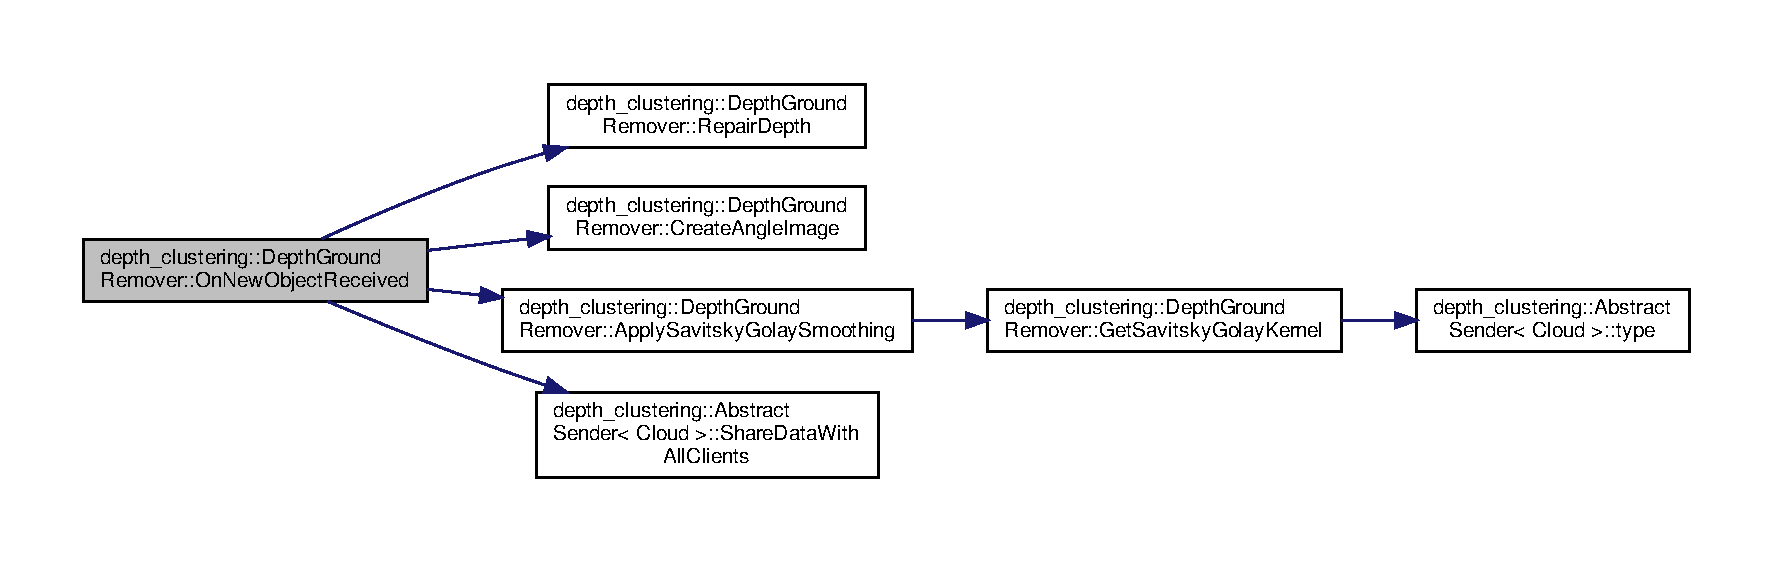
\includegraphics[width=350pt]{classdepth__clustering_1_1DepthGroundRemover_ab2c3bcc8df6cc70ad5057f5ec3bd074f_cgraph}
\end{center}
\end{figure}
\mbox{\Hypertarget{classdepth__clustering_1_1DepthGroundRemover_a51dd313ed1bdda2188fb3a3fa1c5738e}\label{classdepth__clustering_1_1DepthGroundRemover_a51dd313ed1bdda2188fb3a3fa1c5738e}} 
\index{depth\+\_\+clustering\+::\+Depth\+Ground\+Remover@{depth\+\_\+clustering\+::\+Depth\+Ground\+Remover}!Repair\+Depth@{Repair\+Depth}}
\index{Repair\+Depth@{Repair\+Depth}!depth\+\_\+clustering\+::\+Depth\+Ground\+Remover@{depth\+\_\+clustering\+::\+Depth\+Ground\+Remover}}
\subsubsection{\texorpdfstring{Repair\+Depth()}{RepairDepth()}}
{\footnotesize\ttfamily cv\+::\+Mat depth\+\_\+clustering\+::\+Depth\+Ground\+Remover\+::\+Repair\+Depth (\begin{DoxyParamCaption}\item[{const cv\+::\+Mat \&}]{no\+\_\+ground\+\_\+image,  }\item[{int}]{step,  }\item[{float}]{depth\+\_\+threshold }\end{DoxyParamCaption})\hspace{0.3cm}{\ttfamily [protected]}}



Repair zeros in the depth image. 


\begin{DoxyParams}[1]{Parameters}
\mbox{\tt in}  & {\em depth\+\_\+image} & The depth image\\
\hline
\end{DoxyParams}
\begin{DoxyReturn}{Returns}
depth image with repaired values 
\end{DoxyReturn}
Here is the caller graph for this function\+:\nopagebreak
\begin{figure}[H]
\begin{center}
\leavevmode
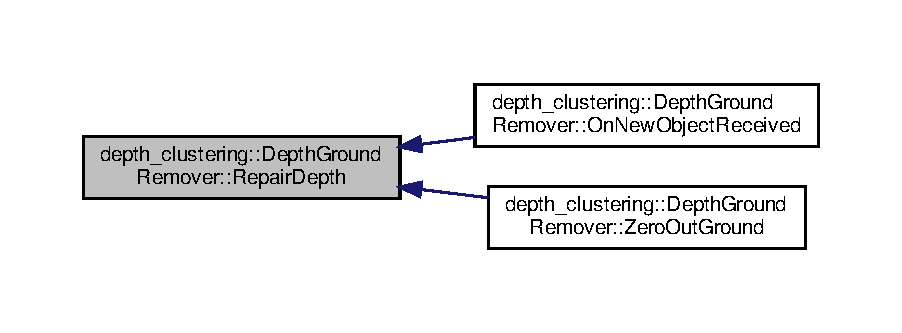
\includegraphics[width=350pt]{classdepth__clustering_1_1DepthGroundRemover_a51dd313ed1bdda2188fb3a3fa1c5738e_icgraph}
\end{center}
\end{figure}
\mbox{\Hypertarget{classdepth__clustering_1_1DepthGroundRemover_a81aa3a52c70223555b4f4e1800e05022}\label{classdepth__clustering_1_1DepthGroundRemover_a81aa3a52c70223555b4f4e1800e05022}} 
\index{depth\+\_\+clustering\+::\+Depth\+Ground\+Remover@{depth\+\_\+clustering\+::\+Depth\+Ground\+Remover}!Zero\+Out\+Ground@{Zero\+Out\+Ground}}
\index{Zero\+Out\+Ground@{Zero\+Out\+Ground}!depth\+\_\+clustering\+::\+Depth\+Ground\+Remover@{depth\+\_\+clustering\+::\+Depth\+Ground\+Remover}}
\subsubsection{\texorpdfstring{Zero\+Out\+Ground()}{ZeroOutGround()}}
{\footnotesize\ttfamily Mat depth\+\_\+clustering\+::\+Depth\+Ground\+Remover\+::\+Zero\+Out\+Ground (\begin{DoxyParamCaption}\item[{const cv\+::\+Mat \&}]{image,  }\item[{const cv\+::\+Mat \&}]{angle\+\_\+image,  }\item[{const Radians \&}]{threshold }\end{DoxyParamCaption}) const\hspace{0.3cm}{\ttfamily [protected]}}



Zero out all pixels that belong to ground. 


\begin{DoxyParams}[1]{Parameters}
\mbox{\tt in}  & {\em image} & Input depth image \\
\hline
\mbox{\tt in}  & {\em angle\+\_\+image} & The angle image \\
\hline
\mbox{\tt in}  & {\em threshold} & angle threshold\\
\hline
\end{DoxyParams}
\begin{DoxyReturn}{Returns}
depth image with 0 instead of ground pixels 
\end{DoxyReturn}
Here is the call graph for this function\+:\nopagebreak
\begin{figure}[H]
\begin{center}
\leavevmode
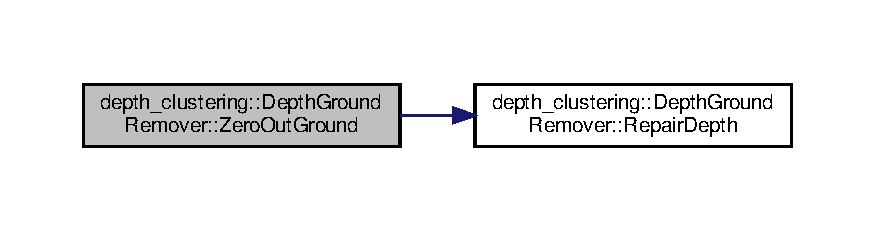
\includegraphics[width=350pt]{classdepth__clustering_1_1DepthGroundRemover_a81aa3a52c70223555b4f4e1800e05022_cgraph}
\end{center}
\end{figure}


The documentation for this class was generated from the following files\+:\begin{DoxyCompactItemize}
\item 
/home/ashwin/catkin\+\_\+ws/src/depth\+\_\+clustering/src/ground\+\_\+removal/depth\+\_\+ground\+\_\+remover.\+h\item 
/home/ashwin/catkin\+\_\+ws/src/depth\+\_\+clustering/src/ground\+\_\+removal/depth\+\_\+ground\+\_\+remover.\+cpp\end{DoxyCompactItemize}

\hypertarget{classdepth__clustering_1_1DijkstraImageLabeler}{}\section{depth\+\_\+clustering\+:\+:Dijkstra\+Image\+Labeler$<$ S\+T\+E\+P\+\_\+\+R\+OW, S\+T\+E\+P\+\_\+\+C\+OL $>$ Class Template Reference}
\label{classdepth__clustering_1_1DijkstraImageLabeler}\index{depth\+\_\+clustering\+::\+Dijkstra\+Image\+Labeler$<$ S\+T\+E\+P\+\_\+\+R\+O\+W, S\+T\+E\+P\+\_\+\+C\+O\+L $>$@{depth\+\_\+clustering\+::\+Dijkstra\+Image\+Labeler$<$ S\+T\+E\+P\+\_\+\+R\+O\+W, S\+T\+E\+P\+\_\+\+C\+O\+L $>$}}


Label image with Dijkstra. Slower, then linear.  




{\ttfamily \#include $<$dijkstra\+\_\+image\+\_\+labeler.\+h$>$}

\subsection*{Public Member Functions}
\begin{DoxyCompactItemize}
\item 
\mbox{\Hypertarget{classdepth__clustering_1_1DijkstraImageLabeler_ac852e1ee20615b3ba62b31a090157cdd}\label{classdepth__clustering_1_1DijkstraImageLabeler_ac852e1ee20615b3ba62b31a090157cdd}} 
{\bfseries Dijkstra\+Image\+Labeler} (const cv\+::\+Mat \&depth\+\_\+image, const \hyperlink{classdepth__clustering_1_1ProjectionParams}{Projection\+Params} \&params, const Radians \&angle\+\_\+threshold)
\item 
\mbox{\Hypertarget{classdepth__clustering_1_1DijkstraImageLabeler_a949206a2cfbf234bb523c0a1bc0fc3ba}\label{classdepth__clustering_1_1DijkstraImageLabeler_a949206a2cfbf234bb523c0a1bc0fc3ba}} 
void \hyperlink{classdepth__clustering_1_1DijkstraImageLabeler_a949206a2cfbf234bb523c0a1bc0fc3ba}{Compute\+Labels} (Diff\+Factory\+::\+Diff\+Type diff\+\_\+type) override
\begin{DoxyCompactList}\small\item\em An interface for children to compute labels. \end{DoxyCompactList}\end{DoxyCompactItemize}
\subsection*{Public Attributes}
\begin{DoxyCompactItemize}
\item 
\mbox{\Hypertarget{classdepth__clustering_1_1DijkstraImageLabeler_ae7c58a8b42e1f17b76e3b48e610a1195}\label{classdepth__clustering_1_1DijkstraImageLabeler_ae7c58a8b42e1f17b76e3b48e610a1195}} 
std\+::array$<$ Pixel\+Coord, N\+E\+I\+G\+H\+\_\+\+S\+I\+ZE $>$ {\bfseries Neighborhood}
\end{DoxyCompactItemize}
\subsection*{Static Public Attributes}
\begin{DoxyCompactItemize}
\item 
\mbox{\Hypertarget{classdepth__clustering_1_1DijkstraImageLabeler_a3a1f1c3b1eac8cb71ff04b9d6cc58ea3}\label{classdepth__clustering_1_1DijkstraImageLabeler_a3a1f1c3b1eac8cb71ff04b9d6cc58ea3}} 
static constexpr int16\+\_\+t {\bfseries N\+E\+I\+G\+H\+\_\+\+S\+I\+ZE} = 2 $\ast$ S\+T\+E\+P\+\_\+\+R\+OW + 2 $\ast$ S\+T\+E\+P\+\_\+\+C\+OL
\end{DoxyCompactItemize}
\subsection*{Additional Inherited Members}


\subsection{Detailed Description}
\subsubsection*{template$<$int16\+\_\+t S\+T\+E\+P\+\_\+\+R\+OW = 1, int16\+\_\+t S\+T\+E\+P\+\_\+\+C\+OL = 1$>$\newline
class depth\+\_\+clustering\+::\+Dijkstra\+Image\+Labeler$<$ S\+T\+E\+P\+\_\+\+R\+O\+W, S\+T\+E\+P\+\_\+\+C\+O\+L $>$}

Label image with Dijkstra. Slower, then linear. 

Inheritance diagram for depth\+\_\+clustering\+:\+:Dijkstra\+Image\+Labeler$<$ S\+T\+E\+P\+\_\+\+R\+OW, S\+T\+E\+P\+\_\+\+C\+OL $>$\+:\nopagebreak
\begin{figure}[H]
\begin{center}
\leavevmode
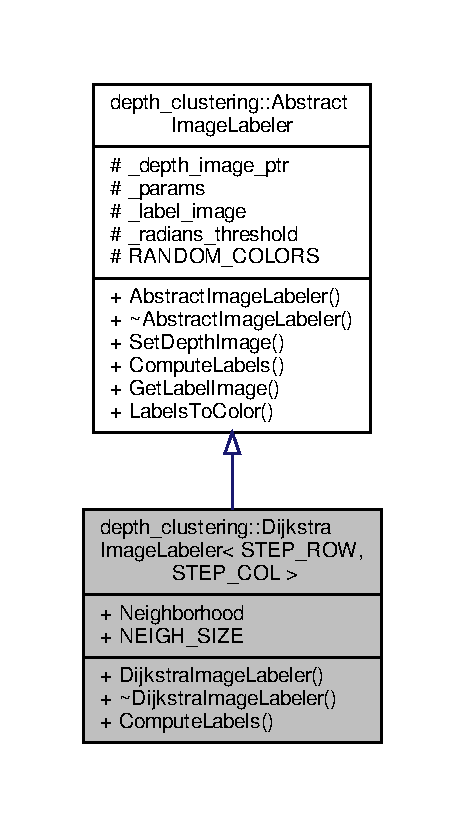
\includegraphics[width=223pt]{classdepth__clustering_1_1DijkstraImageLabeler__inherit__graph}
\end{center}
\end{figure}


Collaboration diagram for depth\+\_\+clustering\+:\+:Dijkstra\+Image\+Labeler$<$ S\+T\+E\+P\+\_\+\+R\+OW, S\+T\+E\+P\+\_\+\+C\+OL $>$\+:\nopagebreak
\begin{figure}[H]
\begin{center}
\leavevmode
\includegraphics[height=550pt]{classdepth__clustering_1_1DijkstraImageLabeler__coll__graph}
\end{center}
\end{figure}


The documentation for this class was generated from the following file\+:\begin{DoxyCompactItemize}
\item 
/home/ashwin/catkin\+\_\+ws/src/depth\+\_\+clustering/src/image\+\_\+labelers/dijkstra\+\_\+image\+\_\+labeler.\+h\end{DoxyCompactItemize}

\hypertarget{classdepth__clustering_1_1EuclideanClusterer}{}\section{depth\+\_\+clustering\+:\+:Euclidean\+Clusterer Class Reference}
\label{classdepth__clustering_1_1EuclideanClusterer}\index{depth\+\_\+clustering\+::\+Euclidean\+Clusterer@{depth\+\_\+clustering\+::\+Euclidean\+Clusterer}}


Class for euclidean clustering.  




{\ttfamily \#include $<$euclidean\+\_\+clusterer.\+h$>$}

\subsection*{Public Types}
\begin{DoxyCompactItemize}
\item 
\mbox{\Hypertarget{classdepth__clustering_1_1EuclideanClusterer_a7c8df2531faab16c7156087cd62d31ca}\label{classdepth__clustering_1_1EuclideanClusterer_a7c8df2531faab16c7156087cd62d31ca}} 
using {\bfseries PointT} = pcl\+::\+Point\+X\+Y\+ZL
\end{DoxyCompactItemize}
\subsection*{Public Member Functions}
\begin{DoxyCompactItemize}
\item 
\mbox{\Hypertarget{classdepth__clustering_1_1EuclideanClusterer_a1c8b10d1977bf4c1f463d2f1942526df}\label{classdepth__clustering_1_1EuclideanClusterer_a1c8b10d1977bf4c1f463d2f1942526df}} 
{\bfseries Euclidean\+Clusterer} (double cluster\+\_\+tollerance=0.\+2, uint16\+\_\+t min\+\_\+cluster\+\_\+size=100, uint16\+\_\+t max\+\_\+cluster\+\_\+size=25000, uint16\+\_\+t skip=10)
\item 
void \hyperlink{classdepth__clustering_1_1EuclideanClusterer_a8ebdd098c514a05f17f16070255b27a6}{On\+New\+Object\+Received} (const \hyperlink{classdepth__clustering_1_1Cloud}{Cloud} \&cloud, const int sender\+\_\+id) override
\begin{DoxyCompactList}\small\item\em Gets called when somebody sends this client an object. \end{DoxyCompactList}\end{DoxyCompactItemize}
\subsection*{Additional Inherited Members}


\subsection{Detailed Description}
Class for euclidean clustering. 

Inheritance diagram for depth\+\_\+clustering\+:\+:Euclidean\+Clusterer\+:\nopagebreak
\begin{figure}[H]
\begin{center}
\leavevmode
\includegraphics[height=550pt]{classdepth__clustering_1_1EuclideanClusterer__inherit__graph}
\end{center}
\end{figure}


Collaboration diagram for depth\+\_\+clustering\+:\+:Euclidean\+Clusterer\+:\nopagebreak
\begin{figure}[H]
\begin{center}
\leavevmode
\includegraphics[height=550pt]{classdepth__clustering_1_1EuclideanClusterer__coll__graph}
\end{center}
\end{figure}


\subsection{Member Function Documentation}
\mbox{\Hypertarget{classdepth__clustering_1_1EuclideanClusterer_a8ebdd098c514a05f17f16070255b27a6}\label{classdepth__clustering_1_1EuclideanClusterer_a8ebdd098c514a05f17f16070255b27a6}} 
\index{depth\+\_\+clustering\+::\+Euclidean\+Clusterer@{depth\+\_\+clustering\+::\+Euclidean\+Clusterer}!On\+New\+Object\+Received@{On\+New\+Object\+Received}}
\index{On\+New\+Object\+Received@{On\+New\+Object\+Received}!depth\+\_\+clustering\+::\+Euclidean\+Clusterer@{depth\+\_\+clustering\+::\+Euclidean\+Clusterer}}
\subsubsection{\texorpdfstring{On\+New\+Object\+Received()}{OnNewObjectReceived()}}
{\footnotesize\ttfamily void depth\+\_\+clustering\+::\+Euclidean\+Clusterer\+::\+On\+New\+Object\+Received (\begin{DoxyParamCaption}\item[{const \hyperlink{classdepth__clustering_1_1Cloud}{Cloud} \&}]{cloud,  }\item[{const int}]{sender\+\_\+id }\end{DoxyParamCaption})\hspace{0.3cm}{\ttfamily [inline]}, {\ttfamily [override]}, {\ttfamily [virtual]}}



Gets called when somebody sends this client an object. 


\begin{DoxyParams}[1]{Parameters}
\mbox{\tt in}  & {\em cloud} & The cloud to cluster \\
\hline
\mbox{\tt in}  & {\em sender\+\_\+id} & The sender identifier \\
\hline
\end{DoxyParams}


Implements \hyperlink{classdepth__clustering_1_1AbstractClient}{depth\+\_\+clustering\+::\+Abstract\+Client$<$ Cloud $>$}.

Here is the call graph for this function\+:\nopagebreak
\begin{figure}[H]
\begin{center}
\leavevmode
\includegraphics[width=350pt]{classdepth__clustering_1_1EuclideanClusterer_a8ebdd098c514a05f17f16070255b27a6_cgraph}
\end{center}
\end{figure}


The documentation for this class was generated from the following file\+:\begin{DoxyCompactItemize}
\item 
/home/ashwin/catkin\+\_\+ws/src/depth\+\_\+clustering/src/clusterers/euclidean\+\_\+clusterer.\+h\end{DoxyCompactItemize}

\hypertarget{classdepth__clustering_1_1FolderReader}{}\section{depth\+\_\+clustering\+:\+:Folder\+Reader Class Reference}
\label{classdepth__clustering_1_1FolderReader}\index{depth\+\_\+clustering\+::\+Folder\+Reader@{depth\+\_\+clustering\+::\+Folder\+Reader}}


Reads a folder and can sort the inputs. Not too efficient.  




{\ttfamily \#include $<$folder\+\_\+reader.\+h$>$}

\subsection*{Public Types}
\begin{DoxyCompactItemize}
\item 
\mbox{\Hypertarget{classdepth__clustering_1_1FolderReader_ab4a3a1cf87192b779ada139a1a00c12a}\label{classdepth__clustering_1_1FolderReader_ab4a3a1cf87192b779ada139a1a00c12a}} 
enum {\bfseries Order} \{ {\bfseries S\+O\+R\+T\+ED}, 
{\bfseries U\+N\+D\+E\+F\+I\+N\+ED}
 \}
\end{DoxyCompactItemize}
\subsection*{Public Member Functions}
\begin{DoxyCompactItemize}
\item 
\mbox{\Hypertarget{classdepth__clustering_1_1FolderReader_a80ae7f477c0ba4ca20e58e0eff0874b2}\label{classdepth__clustering_1_1FolderReader_a80ae7f477c0ba4ca20e58e0eff0874b2}} 
{\bfseries Folder\+Reader} (const std\+::string \&folder\+\_\+path, const std\+::string \&ending\+\_\+with, const Order order=Order\+::\+U\+N\+D\+E\+F\+I\+N\+ED)
\item 
\mbox{\Hypertarget{classdepth__clustering_1_1FolderReader_a298f7b246759d1d926746e057c9d96a0}\label{classdepth__clustering_1_1FolderReader_a298f7b246759d1d926746e057c9d96a0}} 
{\bfseries Folder\+Reader} (const std\+::string \&folder\+\_\+path, const std\+::string \&starting\+\_\+with, const std\+::string \&ending\+\_\+with, const Order order=Order\+::\+U\+N\+D\+E\+F\+I\+N\+ED)
\item 
\mbox{\Hypertarget{classdepth__clustering_1_1FolderReader_aeb4575a662afa48264fec96f4802db90}\label{classdepth__clustering_1_1FolderReader_aeb4575a662afa48264fec96f4802db90}} 
std\+::string {\bfseries Get\+Next\+File\+Path} ()
\item 
\mbox{\Hypertarget{classdepth__clustering_1_1FolderReader_a463cb6564efbad7d6b3000775ba93292}\label{classdepth__clustering_1_1FolderReader_a463cb6564efbad7d6b3000775ba93292}} 
const std\+::vector$<$ std\+::string $>$ \& {\bfseries Get\+All\+File\+Paths} () const
\end{DoxyCompactItemize}
\subsection*{Protected Attributes}
\begin{DoxyCompactItemize}
\item 
\mbox{\Hypertarget{classdepth__clustering_1_1FolderReader_af9ed4e41e57050d7859cd066eb841792}\label{classdepth__clustering_1_1FolderReader_af9ed4e41e57050d7859cd066eb841792}} 
std\+::vector$<$ std\+::string $>$ {\bfseries \+\_\+all\+\_\+paths}
\item 
\mbox{\Hypertarget{classdepth__clustering_1_1FolderReader_aa9fae723281ea00040a803fc15a86d5d}\label{classdepth__clustering_1_1FolderReader_aa9fae723281ea00040a803fc15a86d5d}} 
size\+\_\+t {\bfseries \+\_\+path\+\_\+counter}
\end{DoxyCompactItemize}


\subsection{Detailed Description}
Reads a folder and can sort the inputs. Not too efficient. 

Collaboration diagram for depth\+\_\+clustering\+:\+:Folder\+Reader\+:\nopagebreak
\begin{figure}[H]
\begin{center}
\leavevmode
\includegraphics[width=201pt]{classdepth__clustering_1_1FolderReader__coll__graph}
\end{center}
\end{figure}


The documentation for this class was generated from the following files\+:\begin{DoxyCompactItemize}
\item 
/home/ashwin/catkin\+\_\+ws/src/depth\+\_\+clustering/src/utils/folder\+\_\+reader.\+h\item 
/home/ashwin/catkin\+\_\+ws/src/depth\+\_\+clustering/src/utils/folder\+\_\+reader.\+cpp\end{DoxyCompactItemize}

\hypertarget{classdepth__clustering_1_1Identifiable}{}\section{depth\+\_\+clustering\+:\+:Identifiable Class Reference}
\label{classdepth__clustering_1_1Identifiable}\index{depth\+\_\+clustering\+::\+Identifiable@{depth\+\_\+clustering\+::\+Identifiable}}


Class for identifiable.  




{\ttfamily \#include $<$identifiable.\+h$>$}

\subsection*{Public Member Functions}
\begin{DoxyCompactItemize}
\item 
int \hyperlink{classdepth__clustering_1_1Identifiable_a50f8b49ce7f7f0d9d02f31f74e0fc9e0}{id} () const
\begin{DoxyCompactList}\small\item\em Gets current object id. \end{DoxyCompactList}\item 
virtual std\+::string \hyperlink{classdepth__clustering_1_1Identifiable_a3de92b22eb8d77cf80a50998a84ecd8a}{guess\+\_\+class\+\_\+name} () const
\begin{DoxyCompactList}\small\item\em Guesses class name from typeid. \end{DoxyCompactList}\end{DoxyCompactItemize}
\subsection*{Static Public Member Functions}
\begin{DoxyCompactItemize}
\item 
static int \hyperlink{classdepth__clustering_1_1Identifiable_a7b3be5250a82404765617ba7239041f1}{get\+\_\+current\+\_\+id\+\_\+counter} ()
\begin{DoxyCompactList}\small\item\em Gets the current identifier counter. \end{DoxyCompactList}\end{DoxyCompactItemize}
\subsection*{Static Protected Member Functions}
\begin{DoxyCompactItemize}
\item 
\mbox{\Hypertarget{classdepth__clustering_1_1Identifiable_a61d070e7b5adbef771d5b4df7b9e2f75}\label{classdepth__clustering_1_1Identifiable_a61d070e7b5adbef771d5b4df7b9e2f75}} 
static std\+::string {\bfseries Demangle\+Name} (const char $\ast$tname)
\end{DoxyCompactItemize}
\subsection*{Protected Attributes}
\begin{DoxyCompactItemize}
\item 
\mbox{\Hypertarget{classdepth__clustering_1_1Identifiable_a82e9edccdd02896f9bcd2fa829645158}\label{classdepth__clustering_1_1Identifiable_a82e9edccdd02896f9bcd2fa829645158}} 
const int {\bfseries \+\_\+k\+Id}
\end{DoxyCompactItemize}
\subsection*{Static Protected Attributes}
\begin{DoxyCompactItemize}
\item 
\mbox{\Hypertarget{classdepth__clustering_1_1Identifiable_ac467cc001b2e67e09a10c7dc0da96c4c}\label{classdepth__clustering_1_1Identifiable_ac467cc001b2e67e09a10c7dc0da96c4c}} 
static int {\bfseries Unique\+Id\+Counter} = 0
\end{DoxyCompactItemize}


\subsection{Detailed Description}
Class for identifiable. 

Inheritance diagram for depth\+\_\+clustering\+:\+:Identifiable\+:\nopagebreak
\begin{figure}[H]
\begin{center}
\leavevmode
\includegraphics[width=350pt]{classdepth__clustering_1_1Identifiable__inherit__graph}
\end{center}
\end{figure}


Collaboration diagram for depth\+\_\+clustering\+:\+:Identifiable\+:\nopagebreak
\begin{figure}[H]
\begin{center}
\leavevmode
\includegraphics[width=221pt]{classdepth__clustering_1_1Identifiable__coll__graph}
\end{center}
\end{figure}


\subsection{Member Function Documentation}
\mbox{\Hypertarget{classdepth__clustering_1_1Identifiable_a7b3be5250a82404765617ba7239041f1}\label{classdepth__clustering_1_1Identifiable_a7b3be5250a82404765617ba7239041f1}} 
\index{depth\+\_\+clustering\+::\+Identifiable@{depth\+\_\+clustering\+::\+Identifiable}!get\+\_\+current\+\_\+id\+\_\+counter@{get\+\_\+current\+\_\+id\+\_\+counter}}
\index{get\+\_\+current\+\_\+id\+\_\+counter@{get\+\_\+current\+\_\+id\+\_\+counter}!depth\+\_\+clustering\+::\+Identifiable@{depth\+\_\+clustering\+::\+Identifiable}}
\subsubsection{\texorpdfstring{get\+\_\+current\+\_\+id\+\_\+counter()}{get\_current\_id\_counter()}}
{\footnotesize\ttfamily static int depth\+\_\+clustering\+::\+Identifiable\+::get\+\_\+current\+\_\+id\+\_\+counter (\begin{DoxyParamCaption}{ }\end{DoxyParamCaption})\hspace{0.3cm}{\ttfamily [inline]}, {\ttfamily [static]}}



Gets the current identifier counter. 

\begin{DoxyReturn}{Returns}
The current identifier counter. 
\end{DoxyReturn}
\mbox{\Hypertarget{classdepth__clustering_1_1Identifiable_a3de92b22eb8d77cf80a50998a84ecd8a}\label{classdepth__clustering_1_1Identifiable_a3de92b22eb8d77cf80a50998a84ecd8a}} 
\index{depth\+\_\+clustering\+::\+Identifiable@{depth\+\_\+clustering\+::\+Identifiable}!guess\+\_\+class\+\_\+name@{guess\+\_\+class\+\_\+name}}
\index{guess\+\_\+class\+\_\+name@{guess\+\_\+class\+\_\+name}!depth\+\_\+clustering\+::\+Identifiable@{depth\+\_\+clustering\+::\+Identifiable}}
\subsubsection{\texorpdfstring{guess\+\_\+class\+\_\+name()}{guess\_class\_name()}}
{\footnotesize\ttfamily virtual std\+::string depth\+\_\+clustering\+::\+Identifiable\+::guess\+\_\+class\+\_\+name (\begin{DoxyParamCaption}{ }\end{DoxyParamCaption}) const\hspace{0.3cm}{\ttfamily [inline]}, {\ttfamily [virtual]}}



Guesses class name from typeid. 

\begin{DoxyReturn}{Returns}
Class name as string. 
\end{DoxyReturn}
Here is the caller graph for this function\+:\nopagebreak
\begin{figure}[H]
\begin{center}
\leavevmode
\includegraphics[width=350pt]{classdepth__clustering_1_1Identifiable_a3de92b22eb8d77cf80a50998a84ecd8a_icgraph}
\end{center}
\end{figure}
\mbox{\Hypertarget{classdepth__clustering_1_1Identifiable_a50f8b49ce7f7f0d9d02f31f74e0fc9e0}\label{classdepth__clustering_1_1Identifiable_a50f8b49ce7f7f0d9d02f31f74e0fc9e0}} 
\index{depth\+\_\+clustering\+::\+Identifiable@{depth\+\_\+clustering\+::\+Identifiable}!id@{id}}
\index{id@{id}!depth\+\_\+clustering\+::\+Identifiable@{depth\+\_\+clustering\+::\+Identifiable}}
\subsubsection{\texorpdfstring{id()}{id()}}
{\footnotesize\ttfamily int depth\+\_\+clustering\+::\+Identifiable\+::id (\begin{DoxyParamCaption}{ }\end{DoxyParamCaption}) const\hspace{0.3cm}{\ttfamily [inline]}}



Gets current object id. 

\begin{DoxyReturn}{Returns}
id of the object. 
\end{DoxyReturn}
Here is the caller graph for this function\+:\nopagebreak
\begin{figure}[H]
\begin{center}
\leavevmode
\includegraphics[width=350pt]{classdepth__clustering_1_1Identifiable_a50f8b49ce7f7f0d9d02f31f74e0fc9e0_icgraph}
\end{center}
\end{figure}


The documentation for this class was generated from the following files\+:\begin{DoxyCompactItemize}
\item 
/home/ashwin/catkin\+\_\+ws/src/depth\+\_\+clustering/src/communication/identifiable.\+h\item 
/home/ashwin/catkin\+\_\+ws/src/depth\+\_\+clustering/src/communication/identifiable.\+cpp\end{DoxyCompactItemize}

\hypertarget{classdepth__clustering_1_1ImageBasedClusterer}{}\section{depth\+\_\+clustering\+:\+:Image\+Based\+Clusterer$<$ LabelerT $>$ Class Template Reference}
\label{classdepth__clustering_1_1ImageBasedClusterer}\index{depth\+\_\+clustering\+::\+Image\+Based\+Clusterer$<$ Labeler\+T $>$@{depth\+\_\+clustering\+::\+Image\+Based\+Clusterer$<$ Labeler\+T $>$}}


Class for image based clusterer.  




{\ttfamily \#include $<$image\+\_\+based\+\_\+clusterer.\+h$>$}

\subsection*{Public Types}
\begin{DoxyCompactItemize}
\item 
\mbox{\Hypertarget{classdepth__clustering_1_1ImageBasedClusterer_a62774a9ad3f50dd9811c2194c99eff7f}\label{classdepth__clustering_1_1ImageBasedClusterer_a62774a9ad3f50dd9811c2194c99eff7f}} 
using {\bfseries Receiver} = \hyperlink{classdepth__clustering_1_1AbstractClient}{Abstract\+Client}$<$ \hyperlink{classdepth__clustering_1_1Cloud}{Cloud} $>$
\item 
\mbox{\Hypertarget{classdepth__clustering_1_1ImageBasedClusterer_abafea1c097279afe4f48134d77bac6c6}\label{classdepth__clustering_1_1ImageBasedClusterer_abafea1c097279afe4f48134d77bac6c6}} 
using {\bfseries Sender} = \hyperlink{classdepth__clustering_1_1AbstractSender}{Abstract\+Sender}$<$ std\+::unordered\+\_\+map$<$ uint16\+\_\+t, \hyperlink{classdepth__clustering_1_1Cloud}{Cloud} $>$ $>$
\end{DoxyCompactItemize}
\subsection*{Public Member Functions}
\begin{DoxyCompactItemize}
\item 
\hyperlink{classdepth__clustering_1_1ImageBasedClusterer_a6a8bdd77542e14ee420988ad80579f35}{Image\+Based\+Clusterer} (Radians angle\+\_\+tollerance=8\+\_\+deg, uint16\+\_\+t min\+\_\+cluster\+\_\+size=100, uint16\+\_\+t max\+\_\+cluster\+\_\+size=25000)
\begin{DoxyCompactList}\small\item\em Construct an image-\/based clusterer. \end{DoxyCompactList}\item 
void \hyperlink{classdepth__clustering_1_1ImageBasedClusterer_a0dd114829041816d309d6c8f9ff41cad}{Set\+Diff\+Type} (Diff\+Factory\+::\+Diff\+Type diff\+\_\+type)
\begin{DoxyCompactList}\small\item\em Sets the difference type. \end{DoxyCompactList}\item 
void \hyperlink{classdepth__clustering_1_1ImageBasedClusterer_a6af0de0dad7450c34c655fb447886716}{Set\+Label\+Image\+Client} (\hyperlink{classdepth__clustering_1_1AbstractClient}{Abstract\+Client}$<$ cv\+::\+Mat $>$ $\ast$client)
\begin{DoxyCompactList}\small\item\em Sets the label image client. \end{DoxyCompactList}\item 
void \hyperlink{classdepth__clustering_1_1ImageBasedClusterer_a98e7be00573047a2380ded00bb0542e6}{On\+New\+Object\+Received} (const \hyperlink{classdepth__clustering_1_1Cloud}{Cloud} \&cloud, int) override
\begin{DoxyCompactList}\small\item\em Gets called when clusterer receives a cloud to cluster. \end{DoxyCompactList}\end{DoxyCompactItemize}
\subsection*{Additional Inherited Members}


\subsection{Detailed Description}
\subsubsection*{template$<$typename LabelerT$>$\newline
class depth\+\_\+clustering\+::\+Image\+Based\+Clusterer$<$ Labeler\+T $>$}

Class for image based clusterer. 


\begin{DoxyTemplParams}{Template Parameters}
{\em LabelerT} & A Labeler class to be used for labeling. \\
\hline
\end{DoxyTemplParams}


Inheritance diagram for depth\+\_\+clustering\+:\+:Image\+Based\+Clusterer$<$ LabelerT $>$\+:\nopagebreak
\begin{figure}[H]
\begin{center}
\leavevmode
\includegraphics[height=550pt]{classdepth__clustering_1_1ImageBasedClusterer__inherit__graph}
\end{center}
\end{figure}


Collaboration diagram for depth\+\_\+clustering\+:\+:Image\+Based\+Clusterer$<$ LabelerT $>$\+:\nopagebreak
\begin{figure}[H]
\begin{center}
\leavevmode
\includegraphics[height=550pt]{classdepth__clustering_1_1ImageBasedClusterer__coll__graph}
\end{center}
\end{figure}


\subsection{Constructor \& Destructor Documentation}
\mbox{\Hypertarget{classdepth__clustering_1_1ImageBasedClusterer_a6a8bdd77542e14ee420988ad80579f35}\label{classdepth__clustering_1_1ImageBasedClusterer_a6a8bdd77542e14ee420988ad80579f35}} 
\index{depth\+\_\+clustering\+::\+Image\+Based\+Clusterer@{depth\+\_\+clustering\+::\+Image\+Based\+Clusterer}!Image\+Based\+Clusterer@{Image\+Based\+Clusterer}}
\index{Image\+Based\+Clusterer@{Image\+Based\+Clusterer}!depth\+\_\+clustering\+::\+Image\+Based\+Clusterer@{depth\+\_\+clustering\+::\+Image\+Based\+Clusterer}}
\subsubsection{\texorpdfstring{Image\+Based\+Clusterer()}{ImageBasedClusterer()}}
{\footnotesize\ttfamily template$<$typename LabelerT$>$ \\
\hyperlink{classdepth__clustering_1_1ImageBasedClusterer}{depth\+\_\+clustering\+::\+Image\+Based\+Clusterer}$<$ LabelerT $>$\+::\hyperlink{classdepth__clustering_1_1ImageBasedClusterer}{Image\+Based\+Clusterer} (\begin{DoxyParamCaption}\item[{Radians}]{angle\+\_\+tollerance = {\ttfamily 8\+\_\+deg},  }\item[{uint16\+\_\+t}]{min\+\_\+cluster\+\_\+size = {\ttfamily 100},  }\item[{uint16\+\_\+t}]{max\+\_\+cluster\+\_\+size = {\ttfamily 25000} }\end{DoxyParamCaption})\hspace{0.3cm}{\ttfamily [inline]}, {\ttfamily [explicit]}}



Construct an image-\/based clusterer. 


\begin{DoxyParams}[1]{Parameters}
\mbox{\tt in}  & {\em angle\+\_\+tollerance} & The angle tollerance to separate objects \\
\hline
\mbox{\tt in}  & {\em min\+\_\+cluster\+\_\+size} & The minimum cluster size to send \\
\hline
\mbox{\tt in}  & {\em max\+\_\+cluster\+\_\+size} & The maximum cluster size to send \\
\hline
\end{DoxyParams}


\subsection{Member Function Documentation}
\mbox{\Hypertarget{classdepth__clustering_1_1ImageBasedClusterer_a98e7be00573047a2380ded00bb0542e6}\label{classdepth__clustering_1_1ImageBasedClusterer_a98e7be00573047a2380ded00bb0542e6}} 
\index{depth\+\_\+clustering\+::\+Image\+Based\+Clusterer@{depth\+\_\+clustering\+::\+Image\+Based\+Clusterer}!On\+New\+Object\+Received@{On\+New\+Object\+Received}}
\index{On\+New\+Object\+Received@{On\+New\+Object\+Received}!depth\+\_\+clustering\+::\+Image\+Based\+Clusterer@{depth\+\_\+clustering\+::\+Image\+Based\+Clusterer}}
\subsubsection{\texorpdfstring{On\+New\+Object\+Received()}{OnNewObjectReceived()}}
{\footnotesize\ttfamily template$<$typename LabelerT$>$ \\
void \hyperlink{classdepth__clustering_1_1ImageBasedClusterer}{depth\+\_\+clustering\+::\+Image\+Based\+Clusterer}$<$ LabelerT $>$\+::On\+New\+Object\+Received (\begin{DoxyParamCaption}\item[{const \hyperlink{classdepth__clustering_1_1Cloud}{Cloud} \&}]{cloud,  }\item[{int}]{ }\end{DoxyParamCaption})\hspace{0.3cm}{\ttfamily [inline]}, {\ttfamily [override]}, {\ttfamily [virtual]}}



Gets called when clusterer receives a cloud to cluster. 


\begin{DoxyParams}[1]{Parameters}
\mbox{\tt in}  & {\em cloud} & The cloud to cluster \\
\hline
\mbox{\tt in}  & {\em sender\+\_\+id} & The sender identifier \\
\hline
\end{DoxyParams}


Implements \hyperlink{classdepth__clustering_1_1AbstractClient}{depth\+\_\+clustering\+::\+Abstract\+Client$<$ Cloud $>$}.

\mbox{\Hypertarget{classdepth__clustering_1_1ImageBasedClusterer_a0dd114829041816d309d6c8f9ff41cad}\label{classdepth__clustering_1_1ImageBasedClusterer_a0dd114829041816d309d6c8f9ff41cad}} 
\index{depth\+\_\+clustering\+::\+Image\+Based\+Clusterer@{depth\+\_\+clustering\+::\+Image\+Based\+Clusterer}!Set\+Diff\+Type@{Set\+Diff\+Type}}
\index{Set\+Diff\+Type@{Set\+Diff\+Type}!depth\+\_\+clustering\+::\+Image\+Based\+Clusterer@{depth\+\_\+clustering\+::\+Image\+Based\+Clusterer}}
\subsubsection{\texorpdfstring{Set\+Diff\+Type()}{SetDiffType()}}
{\footnotesize\ttfamily template$<$typename LabelerT$>$ \\
void \hyperlink{classdepth__clustering_1_1ImageBasedClusterer}{depth\+\_\+clustering\+::\+Image\+Based\+Clusterer}$<$ LabelerT $>$\+::Set\+Diff\+Type (\begin{DoxyParamCaption}\item[{Diff\+Factory\+::\+Diff\+Type}]{diff\+\_\+type }\end{DoxyParamCaption})\hspace{0.3cm}{\ttfamily [inline]}}



Sets the difference type. 


\begin{DoxyParams}[1]{Parameters}
\mbox{\tt in}  & {\em diff\+\_\+type} & The difference type \\
\hline
\end{DoxyParams}
\mbox{\Hypertarget{classdepth__clustering_1_1ImageBasedClusterer_a6af0de0dad7450c34c655fb447886716}\label{classdepth__clustering_1_1ImageBasedClusterer_a6af0de0dad7450c34c655fb447886716}} 
\index{depth\+\_\+clustering\+::\+Image\+Based\+Clusterer@{depth\+\_\+clustering\+::\+Image\+Based\+Clusterer}!Set\+Label\+Image\+Client@{Set\+Label\+Image\+Client}}
\index{Set\+Label\+Image\+Client@{Set\+Label\+Image\+Client}!depth\+\_\+clustering\+::\+Image\+Based\+Clusterer@{depth\+\_\+clustering\+::\+Image\+Based\+Clusterer}}
\subsubsection{\texorpdfstring{Set\+Label\+Image\+Client()}{SetLabelImageClient()}}
{\footnotesize\ttfamily template$<$typename LabelerT$>$ \\
void \hyperlink{classdepth__clustering_1_1ImageBasedClusterer}{depth\+\_\+clustering\+::\+Image\+Based\+Clusterer}$<$ LabelerT $>$\+::Set\+Label\+Image\+Client (\begin{DoxyParamCaption}\item[{\hyperlink{classdepth__clustering_1_1AbstractClient}{Abstract\+Client}$<$ cv\+::\+Mat $>$ $\ast$}]{client }\end{DoxyParamCaption})\hspace{0.3cm}{\ttfamily [inline]}}



Sets the label image client. 


\begin{DoxyParams}{Parameters}
{\em client} & The client to receive color images with labels \\
\hline
\end{DoxyParams}


The documentation for this class was generated from the following file\+:\begin{DoxyCompactItemize}
\item 
/home/ashwin/catkin\+\_\+ws/src/depth\+\_\+clustering/src/clusterers/image\+\_\+based\+\_\+clusterer.\+h\end{DoxyCompactItemize}

\hypertarget{classdepth__clustering_1_1LinearImageLabeler}{}\section{depth\+\_\+clustering\+:\+:Linear\+Image\+Labeler$<$ S\+T\+E\+P\+\_\+\+R\+OW, S\+T\+E\+P\+\_\+\+C\+OL $>$ Class Template Reference}
\label{classdepth__clustering_1_1LinearImageLabeler}\index{depth\+\_\+clustering\+::\+Linear\+Image\+Labeler$<$ S\+T\+E\+P\+\_\+\+R\+O\+W, S\+T\+E\+P\+\_\+\+C\+O\+L $>$@{depth\+\_\+clustering\+::\+Linear\+Image\+Labeler$<$ S\+T\+E\+P\+\_\+\+R\+O\+W, S\+T\+E\+P\+\_\+\+C\+O\+L $>$}}


Class for linear image labeler.  




{\ttfamily \#include $<$linear\+\_\+image\+\_\+labeler.\+h$>$}

\subsection*{Public Member Functions}
\begin{DoxyCompactItemize}
\item 
\hyperlink{classdepth__clustering_1_1LinearImageLabeler_ad1026a0b49c300c6415691716b5acb99}{Linear\+Image\+Labeler} (const cv\+::\+Mat \&depth\+\_\+image, const \hyperlink{classdepth__clustering_1_1ProjectionParams}{Projection\+Params} \&params, const Radians \&angle\+\_\+threshold)
\begin{DoxyCompactList}\small\item\em Initialize Linear image labeler. \end{DoxyCompactList}\item 
void \hyperlink{classdepth__clustering_1_1LinearImageLabeler_ac5544f26628a05978a6a989ade6a1cd6}{Label\+One\+Component} (uint16\+\_\+t label, const \hyperlink{structdepth__clustering_1_1PixelCoord}{Pixel\+Coord} \&start, const \hyperlink{classdepth__clustering_1_1AbstractDiff}{Abstract\+Diff} $\ast$diff\+\_\+helper)
\begin{DoxyCompactList}\small\item\em Label a single connected component with B\+FS. Can be done faster if we augment the queue with a hash or smth. \end{DoxyCompactList}\item 
float \hyperlink{classdepth__clustering_1_1LinearImageLabeler_abef293e252cf1afcac619f643f376921}{Depth\+At} (const \hyperlink{structdepth__clustering_1_1PixelCoord}{Pixel\+Coord} \&coord) const
\begin{DoxyCompactList}\small\item\em Gets depth value at pixel. \end{DoxyCompactList}\item 
uint16\+\_\+t \hyperlink{classdepth__clustering_1_1LinearImageLabeler_a4389f0085999f71cc283d6c378a2536a}{Label\+At} (const \hyperlink{structdepth__clustering_1_1PixelCoord}{Pixel\+Coord} \&coord) const
\begin{DoxyCompactList}\small\item\em Gets label of a given pixel. \end{DoxyCompactList}\item 
void \hyperlink{classdepth__clustering_1_1LinearImageLabeler_a4693e920b2245f70206a11e141ddcb8f}{Set\+Label} (const \hyperlink{structdepth__clustering_1_1PixelCoord}{Pixel\+Coord} \&coord, uint16\+\_\+t label)
\begin{DoxyCompactList}\small\item\em Sets label of a given pixel. \end{DoxyCompactList}\item 
\mbox{\Hypertarget{classdepth__clustering_1_1LinearImageLabeler_a0dcf6253650499df0c723caaefc459c5}\label{classdepth__clustering_1_1LinearImageLabeler_a0dcf6253650499df0c723caaefc459c5}} 
int16\+\_\+t \hyperlink{classdepth__clustering_1_1LinearImageLabeler_a0dcf6253650499df0c723caaefc459c5}{Wrap\+Cols} (int16\+\_\+t col) const
\begin{DoxyCompactList}\small\item\em Wrap columns around image. \end{DoxyCompactList}\item 
\mbox{\Hypertarget{classdepth__clustering_1_1LinearImageLabeler_a987cca7d9daab304af4bcc448bf6de0f}\label{classdepth__clustering_1_1LinearImageLabeler_a987cca7d9daab304af4bcc448bf6de0f}} 
void \hyperlink{classdepth__clustering_1_1LinearImageLabeler_a987cca7d9daab304af4bcc448bf6de0f}{Compute\+Labels} (Diff\+Factory\+::\+Diff\+Type diff\+\_\+type) override
\begin{DoxyCompactList}\small\item\em Calculates the labels running over the whole image. \end{DoxyCompactList}\end{DoxyCompactItemize}
\subsection*{Public Attributes}
\begin{DoxyCompactItemize}
\item 
\mbox{\Hypertarget{classdepth__clustering_1_1LinearImageLabeler_a7237797a8c13b16aa3cdefe913d8c938}\label{classdepth__clustering_1_1LinearImageLabeler_a7237797a8c13b16aa3cdefe913d8c938}} 
std\+::array$<$ \hyperlink{structdepth__clustering_1_1PixelCoord}{Pixel\+Coord}, N\+E\+I\+G\+H\+\_\+\+S\+I\+ZE $>$ {\bfseries Neighborhood}
\end{DoxyCompactItemize}
\subsection*{Static Public Attributes}
\begin{DoxyCompactItemize}
\item 
\mbox{\Hypertarget{classdepth__clustering_1_1LinearImageLabeler_ad6a78dde18091847582a7cea428ed5fb}\label{classdepth__clustering_1_1LinearImageLabeler_ad6a78dde18091847582a7cea428ed5fb}} 
static constexpr int16\+\_\+t {\bfseries N\+E\+I\+G\+H\+\_\+\+S\+I\+ZE} = 2 $\ast$ S\+T\+E\+P\+\_\+\+R\+OW + 2 $\ast$ S\+T\+E\+P\+\_\+\+C\+OL
\end{DoxyCompactItemize}
\subsection*{Additional Inherited Members}


\subsection{Detailed Description}
\subsubsection*{template$<$int16\+\_\+t S\+T\+E\+P\+\_\+\+R\+OW = 1, int16\+\_\+t S\+T\+E\+P\+\_\+\+C\+OL = 1$>$\newline
class depth\+\_\+clustering\+::\+Linear\+Image\+Labeler$<$ S\+T\+E\+P\+\_\+\+R\+O\+W, S\+T\+E\+P\+\_\+\+C\+O\+L $>$}

Class for linear image labeler. 


\begin{DoxyTemplParams}{Template Parameters}
{\em S\+T\+E\+P\+\_\+\+R\+OW} & step we do over image over rows \\
\hline
{\em S\+T\+E\+P\+\_\+\+C\+OL} & step we do over image over cols \\
\hline
\end{DoxyTemplParams}


Inheritance diagram for depth\+\_\+clustering\+:\+:Linear\+Image\+Labeler$<$ S\+T\+E\+P\+\_\+\+R\+OW, S\+T\+E\+P\+\_\+\+C\+OL $>$\+:\nopagebreak
\begin{figure}[H]
\begin{center}
\leavevmode
\includegraphics[width=223pt]{classdepth__clustering_1_1LinearImageLabeler__inherit__graph}
\end{center}
\end{figure}


Collaboration diagram for depth\+\_\+clustering\+:\+:Linear\+Image\+Labeler$<$ S\+T\+E\+P\+\_\+\+R\+OW, S\+T\+E\+P\+\_\+\+C\+OL $>$\+:\nopagebreak
\begin{figure}[H]
\begin{center}
\leavevmode
\includegraphics[height=550pt]{classdepth__clustering_1_1LinearImageLabeler__coll__graph}
\end{center}
\end{figure}


\subsection{Constructor \& Destructor Documentation}
\mbox{\Hypertarget{classdepth__clustering_1_1LinearImageLabeler_ad1026a0b49c300c6415691716b5acb99}\label{classdepth__clustering_1_1LinearImageLabeler_ad1026a0b49c300c6415691716b5acb99}} 
\index{depth\+\_\+clustering\+::\+Linear\+Image\+Labeler@{depth\+\_\+clustering\+::\+Linear\+Image\+Labeler}!Linear\+Image\+Labeler@{Linear\+Image\+Labeler}}
\index{Linear\+Image\+Labeler@{Linear\+Image\+Labeler}!depth\+\_\+clustering\+::\+Linear\+Image\+Labeler@{depth\+\_\+clustering\+::\+Linear\+Image\+Labeler}}
\subsubsection{\texorpdfstring{Linear\+Image\+Labeler()}{LinearImageLabeler()}}
{\footnotesize\ttfamily template$<$int16\+\_\+t S\+T\+E\+P\+\_\+\+R\+OW = 1, int16\+\_\+t S\+T\+E\+P\+\_\+\+C\+OL = 1$>$ \\
\hyperlink{classdepth__clustering_1_1LinearImageLabeler}{depth\+\_\+clustering\+::\+Linear\+Image\+Labeler}$<$ S\+T\+E\+P\+\_\+\+R\+OW, S\+T\+E\+P\+\_\+\+C\+OL $>$\+::\hyperlink{classdepth__clustering_1_1LinearImageLabeler}{Linear\+Image\+Labeler} (\begin{DoxyParamCaption}\item[{const cv\+::\+Mat \&}]{depth\+\_\+image,  }\item[{const \hyperlink{classdepth__clustering_1_1ProjectionParams}{Projection\+Params} \&}]{params,  }\item[{const Radians \&}]{angle\+\_\+threshold }\end{DoxyParamCaption})\hspace{0.3cm}{\ttfamily [inline]}, {\ttfamily [explicit]}}



Initialize Linear image labeler. 


\begin{DoxyParams}[1]{Parameters}
\mbox{\tt in}  & {\em depth\+\_\+image} & The depth image \\
\hline
\mbox{\tt in}  & {\em params} & The projection parameters \\
\hline
\mbox{\tt in}  & {\em angle\+\_\+threshold} & The angle threshold to seaparate clusters \\
\hline
\end{DoxyParams}


\subsection{Member Function Documentation}
\mbox{\Hypertarget{classdepth__clustering_1_1LinearImageLabeler_abef293e252cf1afcac619f643f376921}\label{classdepth__clustering_1_1LinearImageLabeler_abef293e252cf1afcac619f643f376921}} 
\index{depth\+\_\+clustering\+::\+Linear\+Image\+Labeler@{depth\+\_\+clustering\+::\+Linear\+Image\+Labeler}!Depth\+At@{Depth\+At}}
\index{Depth\+At@{Depth\+At}!depth\+\_\+clustering\+::\+Linear\+Image\+Labeler@{depth\+\_\+clustering\+::\+Linear\+Image\+Labeler}}
\subsubsection{\texorpdfstring{Depth\+At()}{DepthAt()}}
{\footnotesize\ttfamily template$<$int16\+\_\+t S\+T\+E\+P\+\_\+\+R\+OW = 1, int16\+\_\+t S\+T\+E\+P\+\_\+\+C\+OL = 1$>$ \\
float \hyperlink{classdepth__clustering_1_1LinearImageLabeler}{depth\+\_\+clustering\+::\+Linear\+Image\+Labeler}$<$ S\+T\+E\+P\+\_\+\+R\+OW, S\+T\+E\+P\+\_\+\+C\+OL $>$\+::Depth\+At (\begin{DoxyParamCaption}\item[{const \hyperlink{structdepth__clustering_1_1PixelCoord}{Pixel\+Coord} \&}]{coord }\end{DoxyParamCaption}) const\hspace{0.3cm}{\ttfamily [inline]}}



Gets depth value at pixel. 


\begin{DoxyParams}[1]{Parameters}
\mbox{\tt in}  & {\em coord} & Pixel coordinate\\
\hline
\end{DoxyParams}
\begin{DoxyReturn}{Returns}
depth at pixel 
\end{DoxyReturn}
Here is the caller graph for this function\+:\nopagebreak
\begin{figure}[H]
\begin{center}
\leavevmode
\includegraphics[width=350pt]{classdepth__clustering_1_1LinearImageLabeler_abef293e252cf1afcac619f643f376921_icgraph}
\end{center}
\end{figure}
\mbox{\Hypertarget{classdepth__clustering_1_1LinearImageLabeler_a4389f0085999f71cc283d6c378a2536a}\label{classdepth__clustering_1_1LinearImageLabeler_a4389f0085999f71cc283d6c378a2536a}} 
\index{depth\+\_\+clustering\+::\+Linear\+Image\+Labeler@{depth\+\_\+clustering\+::\+Linear\+Image\+Labeler}!Label\+At@{Label\+At}}
\index{Label\+At@{Label\+At}!depth\+\_\+clustering\+::\+Linear\+Image\+Labeler@{depth\+\_\+clustering\+::\+Linear\+Image\+Labeler}}
\subsubsection{\texorpdfstring{Label\+At()}{LabelAt()}}
{\footnotesize\ttfamily template$<$int16\+\_\+t S\+T\+E\+P\+\_\+\+R\+OW = 1, int16\+\_\+t S\+T\+E\+P\+\_\+\+C\+OL = 1$>$ \\
uint16\+\_\+t \hyperlink{classdepth__clustering_1_1LinearImageLabeler}{depth\+\_\+clustering\+::\+Linear\+Image\+Labeler}$<$ S\+T\+E\+P\+\_\+\+R\+OW, S\+T\+E\+P\+\_\+\+C\+OL $>$\+::Label\+At (\begin{DoxyParamCaption}\item[{const \hyperlink{structdepth__clustering_1_1PixelCoord}{Pixel\+Coord} \&}]{coord }\end{DoxyParamCaption}) const\hspace{0.3cm}{\ttfamily [inline]}}



Gets label of a given pixel. 


\begin{DoxyParams}[1]{Parameters}
\mbox{\tt in}  & {\em coord} & Pixel coordinate\\
\hline
\end{DoxyParams}
\begin{DoxyReturn}{Returns}
label for pixel 
\end{DoxyReturn}
Here is the caller graph for this function\+:\nopagebreak
\begin{figure}[H]
\begin{center}
\leavevmode
\includegraphics[width=350pt]{classdepth__clustering_1_1LinearImageLabeler_a4389f0085999f71cc283d6c378a2536a_icgraph}
\end{center}
\end{figure}
\mbox{\Hypertarget{classdepth__clustering_1_1LinearImageLabeler_ac5544f26628a05978a6a989ade6a1cd6}\label{classdepth__clustering_1_1LinearImageLabeler_ac5544f26628a05978a6a989ade6a1cd6}} 
\index{depth\+\_\+clustering\+::\+Linear\+Image\+Labeler@{depth\+\_\+clustering\+::\+Linear\+Image\+Labeler}!Label\+One\+Component@{Label\+One\+Component}}
\index{Label\+One\+Component@{Label\+One\+Component}!depth\+\_\+clustering\+::\+Linear\+Image\+Labeler@{depth\+\_\+clustering\+::\+Linear\+Image\+Labeler}}
\subsubsection{\texorpdfstring{Label\+One\+Component()}{LabelOneComponent()}}
{\footnotesize\ttfamily template$<$int16\+\_\+t S\+T\+E\+P\+\_\+\+R\+OW = 1, int16\+\_\+t S\+T\+E\+P\+\_\+\+C\+OL = 1$>$ \\
void \hyperlink{classdepth__clustering_1_1LinearImageLabeler}{depth\+\_\+clustering\+::\+Linear\+Image\+Labeler}$<$ S\+T\+E\+P\+\_\+\+R\+OW, S\+T\+E\+P\+\_\+\+C\+OL $>$\+::Label\+One\+Component (\begin{DoxyParamCaption}\item[{uint16\+\_\+t}]{label,  }\item[{const \hyperlink{structdepth__clustering_1_1PixelCoord}{Pixel\+Coord} \&}]{start,  }\item[{const \hyperlink{classdepth__clustering_1_1AbstractDiff}{Abstract\+Diff} $\ast$}]{diff\+\_\+helper }\end{DoxyParamCaption})\hspace{0.3cm}{\ttfamily [inline]}}



Label a single connected component with B\+FS. Can be done faster if we augment the queue with a hash or smth. 


\begin{DoxyParams}[1]{Parameters}
\mbox{\tt in}  & {\em label} & Label this component with this label \\
\hline
\mbox{\tt in}  & {\em start} & Start pixel \\
\hline
\mbox{\tt in}  & {\em diff\+\_\+helper} & The difference helper \\
\hline
\end{DoxyParams}
Here is the call graph for this function\+:\nopagebreak
\begin{figure}[H]
\begin{center}
\leavevmode
\includegraphics[width=350pt]{classdepth__clustering_1_1LinearImageLabeler_ac5544f26628a05978a6a989ade6a1cd6_cgraph}
\end{center}
\end{figure}
Here is the caller graph for this function\+:\nopagebreak
\begin{figure}[H]
\begin{center}
\leavevmode
\includegraphics[width=350pt]{classdepth__clustering_1_1LinearImageLabeler_ac5544f26628a05978a6a989ade6a1cd6_icgraph}
\end{center}
\end{figure}
\mbox{\Hypertarget{classdepth__clustering_1_1LinearImageLabeler_a4693e920b2245f70206a11e141ddcb8f}\label{classdepth__clustering_1_1LinearImageLabeler_a4693e920b2245f70206a11e141ddcb8f}} 
\index{depth\+\_\+clustering\+::\+Linear\+Image\+Labeler@{depth\+\_\+clustering\+::\+Linear\+Image\+Labeler}!Set\+Label@{Set\+Label}}
\index{Set\+Label@{Set\+Label}!depth\+\_\+clustering\+::\+Linear\+Image\+Labeler@{depth\+\_\+clustering\+::\+Linear\+Image\+Labeler}}
\subsubsection{\texorpdfstring{Set\+Label()}{SetLabel()}}
{\footnotesize\ttfamily template$<$int16\+\_\+t S\+T\+E\+P\+\_\+\+R\+OW = 1, int16\+\_\+t S\+T\+E\+P\+\_\+\+C\+OL = 1$>$ \\
void \hyperlink{classdepth__clustering_1_1LinearImageLabeler}{depth\+\_\+clustering\+::\+Linear\+Image\+Labeler}$<$ S\+T\+E\+P\+\_\+\+R\+OW, S\+T\+E\+P\+\_\+\+C\+OL $>$\+::Set\+Label (\begin{DoxyParamCaption}\item[{const \hyperlink{structdepth__clustering_1_1PixelCoord}{Pixel\+Coord} \&}]{coord,  }\item[{uint16\+\_\+t}]{label }\end{DoxyParamCaption})\hspace{0.3cm}{\ttfamily [inline]}}



Sets label of a given pixel. 


\begin{DoxyParams}[1]{Parameters}
\mbox{\tt in}  & {\em coord} & Pixel coordinate \\
\hline
\end{DoxyParams}
Here is the caller graph for this function\+:\nopagebreak
\begin{figure}[H]
\begin{center}
\leavevmode
\includegraphics[width=350pt]{classdepth__clustering_1_1LinearImageLabeler_a4693e920b2245f70206a11e141ddcb8f_icgraph}
\end{center}
\end{figure}


The documentation for this class was generated from the following file\+:\begin{DoxyCompactItemize}
\item 
/home/ashwin/catkin\+\_\+ws/src/depth\+\_\+clustering/src/image\+\_\+labelers/linear\+\_\+image\+\_\+labeler.\+h\end{DoxyCompactItemize}

\hypertarget{classdepth__clustering_1_1LineDistDiff}{}\section{depth\+\_\+clustering\+:\+:Line\+Dist\+Diff Class Reference}
\label{classdepth__clustering_1_1LineDistDiff}\index{depth\+\_\+clustering\+::\+Line\+Dist\+Diff@{depth\+\_\+clustering\+::\+Line\+Dist\+Diff}}


Class for line-\/based difference. It is very alike to \hyperlink{classdepth__clustering_1_1AngleDiff}{Angle\+Diff} class, just that after we have computed the angle, we compute $d_1 sin(\beta)$ to get the distance to the line spawned with two measurements.  




{\ttfamily \#include $<$line\+\_\+dist\+\_\+diff.\+h$>$}

\subsection*{Public Member Functions}
\begin{DoxyCompactItemize}
\item 
\hyperlink{classdepth__clustering_1_1LineDistDiff_af922d3e19bc52a2fdbf36317fc474d88}{Line\+Dist\+Diff} (const cv\+::\+Mat $\ast$source\+\_\+image, const \hyperlink{classdepth__clustering_1_1ProjectionParams}{Projection\+Params} $\ast$params)
\begin{DoxyCompactList}\small\item\em Precompute the line distances to avoid losing time on that. \end{DoxyCompactList}\item 
float \hyperlink{classdepth__clustering_1_1LineDistDiff_a839eee44b14de26d85e6dbad5e37b356}{Diff\+At} (const \hyperlink{structdepth__clustering_1_1PixelCoord}{Pixel\+Coord} \&from, const \hyperlink{structdepth__clustering_1_1PixelCoord}{Pixel\+Coord} \&to) const override
\begin{DoxyCompactList}\small\item\em Compute angle-\/based difference. See paper for details. \end{DoxyCompactList}\item 
\mbox{\Hypertarget{classdepth__clustering_1_1LineDistDiff_ae9debede2cffd6bb40ca4c4a82c52f61}\label{classdepth__clustering_1_1LineDistDiff_ae9debede2cffd6bb40ca4c4a82c52f61}} 
bool \hyperlink{classdepth__clustering_1_1LineDistDiff_ae9debede2cffd6bb40ca4c4a82c52f61}{Satisfies\+Threshold} (float angle, float threshold) const override
\begin{DoxyCompactList}\small\item\em Threshold is satisfied if angle is B\+I\+G\+G\+ER than threshold. \end{DoxyCompactList}\item 
cv\+::\+Mat \hyperlink{classdepth__clustering_1_1LineDistDiff_a7feaf820589ccfb47786d5124a74d725}{Visualize} () const override
\begin{DoxyCompactList}\small\item\em Visualize $\beta$ angles as a {\ttfamily cv\+::\+Mat} color image. \end{DoxyCompactList}\end{DoxyCompactItemize}
\subsection*{Additional Inherited Members}


\subsection{Detailed Description}
Class for line-\/based difference. It is very alike to \hyperlink{classdepth__clustering_1_1AngleDiff}{Angle\+Diff} class, just that after we have computed the angle, we compute $d_1 sin(\beta)$ to get the distance to the line spawned with two measurements. 

Inheritance diagram for depth\+\_\+clustering\+:\+:Line\+Dist\+Diff\+:\nopagebreak
\begin{figure}[H]
\begin{center}
\leavevmode
\includegraphics[width=226pt]{classdepth__clustering_1_1LineDistDiff__inherit__graph}
\end{center}
\end{figure}


Collaboration diagram for depth\+\_\+clustering\+:\+:Line\+Dist\+Diff\+:\nopagebreak
\begin{figure}[H]
\begin{center}
\leavevmode
\includegraphics[width=226pt]{classdepth__clustering_1_1LineDistDiff__coll__graph}
\end{center}
\end{figure}


\subsection{Constructor \& Destructor Documentation}
\mbox{\Hypertarget{classdepth__clustering_1_1LineDistDiff_af922d3e19bc52a2fdbf36317fc474d88}\label{classdepth__clustering_1_1LineDistDiff_af922d3e19bc52a2fdbf36317fc474d88}} 
\index{depth\+\_\+clustering\+::\+Line\+Dist\+Diff@{depth\+\_\+clustering\+::\+Line\+Dist\+Diff}!Line\+Dist\+Diff@{Line\+Dist\+Diff}}
\index{Line\+Dist\+Diff@{Line\+Dist\+Diff}!depth\+\_\+clustering\+::\+Line\+Dist\+Diff@{depth\+\_\+clustering\+::\+Line\+Dist\+Diff}}
\subsubsection{\texorpdfstring{Line\+Dist\+Diff()}{LineDistDiff()}}
{\footnotesize\ttfamily depth\+\_\+clustering\+::\+Line\+Dist\+Diff\+::\+Line\+Dist\+Diff (\begin{DoxyParamCaption}\item[{const cv\+::\+Mat $\ast$}]{source\+\_\+image,  }\item[{const \hyperlink{classdepth__clustering_1_1ProjectionParams}{Projection\+Params} $\ast$}]{params }\end{DoxyParamCaption})}



Precompute the line distances to avoid losing time on that. 


\begin{DoxyParams}[1]{Parameters}
\mbox{\tt in}  & {\em source\+\_\+image} & The source image \\
\hline
\mbox{\tt in}  & {\em params} & The projection parameters \\
\hline
\end{DoxyParams}


\subsection{Member Function Documentation}
\mbox{\Hypertarget{classdepth__clustering_1_1LineDistDiff_a839eee44b14de26d85e6dbad5e37b356}\label{classdepth__clustering_1_1LineDistDiff_a839eee44b14de26d85e6dbad5e37b356}} 
\index{depth\+\_\+clustering\+::\+Line\+Dist\+Diff@{depth\+\_\+clustering\+::\+Line\+Dist\+Diff}!Diff\+At@{Diff\+At}}
\index{Diff\+At@{Diff\+At}!depth\+\_\+clustering\+::\+Line\+Dist\+Diff@{depth\+\_\+clustering\+::\+Line\+Dist\+Diff}}
\subsubsection{\texorpdfstring{Diff\+At()}{DiffAt()}}
{\footnotesize\ttfamily float depth\+\_\+clustering\+::\+Line\+Dist\+Diff\+::\+Diff\+At (\begin{DoxyParamCaption}\item[{const \hyperlink{structdepth__clustering_1_1PixelCoord}{Pixel\+Coord} \&}]{from,  }\item[{const \hyperlink{structdepth__clustering_1_1PixelCoord}{Pixel\+Coord} \&}]{to }\end{DoxyParamCaption}) const\hspace{0.3cm}{\ttfamily [override]}, {\ttfamily [virtual]}}



Compute angle-\/based difference. See paper for details. 


\begin{DoxyParams}[1]{Parameters}
\mbox{\tt in}  & {\em from} & Pixel from which to compute difference \\
\hline
\mbox{\tt in}  & {\em to} & Pixel to which to compute difference\\
\hline
\end{DoxyParams}
\begin{DoxyReturn}{Returns}
Angle difference between the values 
\end{DoxyReturn}


Implements \hyperlink{classdepth__clustering_1_1AbstractDiff_a06ba188d8d83d0e4bad66c833656c26d}{depth\+\_\+clustering\+::\+Abstract\+Diff}.

Here is the call graph for this function\+:\nopagebreak
\begin{figure}[H]
\begin{center}
\leavevmode
\includegraphics[width=350pt]{classdepth__clustering_1_1LineDistDiff_a839eee44b14de26d85e6dbad5e37b356_cgraph}
\end{center}
\end{figure}
\mbox{\Hypertarget{classdepth__clustering_1_1LineDistDiff_a7feaf820589ccfb47786d5124a74d725}\label{classdepth__clustering_1_1LineDistDiff_a7feaf820589ccfb47786d5124a74d725}} 
\index{depth\+\_\+clustering\+::\+Line\+Dist\+Diff@{depth\+\_\+clustering\+::\+Line\+Dist\+Diff}!Visualize@{Visualize}}
\index{Visualize@{Visualize}!depth\+\_\+clustering\+::\+Line\+Dist\+Diff@{depth\+\_\+clustering\+::\+Line\+Dist\+Diff}}
\subsubsection{\texorpdfstring{Visualize()}{Visualize()}}
{\footnotesize\ttfamily cv\+::\+Mat depth\+\_\+clustering\+::\+Line\+Dist\+Diff\+::\+Visualize (\begin{DoxyParamCaption}{ }\end{DoxyParamCaption}) const\hspace{0.3cm}{\ttfamily [inline]}, {\ttfamily [override]}, {\ttfamily [virtual]}}



Visualize $\beta$ angles as a {\ttfamily cv\+::\+Mat} color image. 

\begin{DoxyReturn}{Returns}
{\ttfamily cv\+::\+Mat} color image with red channel showing $\beta$ angles in row direction and green channel in col direction. 
\end{DoxyReturn}


Reimplemented from \hyperlink{classdepth__clustering_1_1AbstractDiff_a45314bf711f35e53590af28bdfc45313}{depth\+\_\+clustering\+::\+Abstract\+Diff}.

Here is the caller graph for this function\+:\nopagebreak
\begin{figure}[H]
\begin{center}
\leavevmode
\includegraphics[width=350pt]{classdepth__clustering_1_1LineDistDiff_a7feaf820589ccfb47786d5124a74d725_icgraph}
\end{center}
\end{figure}


The documentation for this class was generated from the following files\+:\begin{DoxyCompactItemize}
\item 
/home/ashwin/catkin\+\_\+ws/src/depth\+\_\+clustering/src/image\+\_\+labelers/diff\+\_\+helpers/line\+\_\+dist\+\_\+diff.\+h\item 
/home/ashwin/catkin\+\_\+ws/src/depth\+\_\+clustering/src/image\+\_\+labelers/diff\+\_\+helpers/line\+\_\+dist\+\_\+diff.\+cpp\end{DoxyCompactItemize}

\hypertarget{classdepth__clustering_1_1LineDistDiffPrecomputed}{}\section{depth\+\_\+clustering\+:\+:Line\+Dist\+Diff\+Precomputed Class Reference}
\label{classdepth__clustering_1_1LineDistDiffPrecomputed}\index{depth\+\_\+clustering\+::\+Line\+Dist\+Diff\+Precomputed@{depth\+\_\+clustering\+::\+Line\+Dist\+Diff\+Precomputed}}


Class for angle difference.  




{\ttfamily \#include $<$line\+\_\+dist\+\_\+diff.\+h$>$}

\subsection*{Public Member Functions}
\begin{DoxyCompactItemize}
\item 
\hyperlink{classdepth__clustering_1_1LineDistDiffPrecomputed_a035909e1718ad9b54b9b4116bbb6c408}{Line\+Dist\+Diff\+Precomputed} (const cv\+::\+Mat $\ast$source\+\_\+image, const \hyperlink{classdepth__clustering_1_1ProjectionParams}{Projection\+Params} $\ast$params)
\begin{DoxyCompactList}\small\item\em Precompute the angles to avoid losing time on that. \end{DoxyCompactList}\item 
float \hyperlink{classdepth__clustering_1_1LineDistDiffPrecomputed_ac505afaa537656af1bcc342ab1e910c4}{Diff\+At} (const \hyperlink{structdepth__clustering_1_1PixelCoord}{Pixel\+Coord} \&from, const \hyperlink{structdepth__clustering_1_1PixelCoord}{Pixel\+Coord} \&to) const override
\begin{DoxyCompactList}\small\item\em Compute angle-\/based difference. See paper for details. Only one of the following situations is possible\+: \end{DoxyCompactList}\item 
\mbox{\Hypertarget{classdepth__clustering_1_1LineDistDiffPrecomputed_ac3ce8196d5e6f49f3e3bdc3e3b32b033}\label{classdepth__clustering_1_1LineDistDiffPrecomputed_ac3ce8196d5e6f49f3e3bdc3e3b32b033}} 
bool \hyperlink{classdepth__clustering_1_1LineDistDiffPrecomputed_ac3ce8196d5e6f49f3e3bdc3e3b32b033}{Satisfies\+Threshold} (float angle, float threshold) const override
\begin{DoxyCompactList}\small\item\em Threshold is satisfied if angle is B\+I\+G\+G\+ER than threshold. \end{DoxyCompactList}\item 
cv\+::\+Mat \hyperlink{classdepth__clustering_1_1LineDistDiffPrecomputed_a77c9cf3bea954f13cd2fef4f8a182425}{Visualize} () const
\begin{DoxyCompactList}\small\item\em Visualize $\beta$ angles as a {\ttfamily cv\+::\+Mat} color image. \end{DoxyCompactList}\end{DoxyCompactItemize}
\subsection*{Protected Member Functions}
\begin{DoxyCompactItemize}
\item 
\mbox{\Hypertarget{classdepth__clustering_1_1LineDistDiffPrecomputed_a9e52e2a94d9f92567953a765475d62a0}\label{classdepth__clustering_1_1LineDistDiffPrecomputed_a9e52e2a94d9f92567953a765475d62a0}} 
void \hyperlink{classdepth__clustering_1_1LineDistDiffPrecomputed_a9e52e2a94d9f92567953a765475d62a0}{Pre\+Compute\+Alpha\+Vecs} ()
\begin{DoxyCompactList}\small\item\em Pre-\/compute values for angles for all cols and rows. \end{DoxyCompactList}\item 
void \hyperlink{classdepth__clustering_1_1LineDistDiffPrecomputed_a9d0211af30be1f60ef4e8db570128a7b}{Pre\+Compute\+Line\+Dists} ()
\begin{DoxyCompactList}\small\item\em Precompute all $\beta$ angles for the image. It generates two matrices for row-\/wise and col-\/wise angles. See picture for illustration. The squares store values of angles between pixels with computation direction shown by arrows. Note that the columns matrix wraps around, i.\+e. the last element stores the difference in angles between the last pixel of the original image and the first one. \end{DoxyCompactList}\item 
float \hyperlink{classdepth__clustering_1_1LineDistDiffPrecomputed_a2725113f6eb03b937104f325adf0c7aa}{Get\+Line\+Dist} (float alpha, float current\+\_\+depth, float neighbor\+\_\+depth) const
\begin{DoxyCompactList}\small\item\em Compute the angle $\beta$ of incline of the line spawned by two given beams. \end{DoxyCompactList}\end{DoxyCompactItemize}
\subsection*{Protected Attributes}
\begin{DoxyCompactItemize}
\item 
\mbox{\Hypertarget{classdepth__clustering_1_1LineDistDiffPrecomputed_aeb0f0894cc1f1fcbd9d40813005432f3}\label{classdepth__clustering_1_1LineDistDiffPrecomputed_aeb0f0894cc1f1fcbd9d40813005432f3}} 
const \hyperlink{classdepth__clustering_1_1ProjectionParams}{Projection\+Params} $\ast$ {\bfseries \+\_\+params} = nullptr
\item 
\mbox{\Hypertarget{classdepth__clustering_1_1LineDistDiffPrecomputed_a5694d6392f56f8659f048f6df7f0ba93}\label{classdepth__clustering_1_1LineDistDiffPrecomputed_a5694d6392f56f8659f048f6df7f0ba93}} 
std\+::vector$<$ float $>$ {\bfseries \+\_\+row\+\_\+alphas}
\item 
\mbox{\Hypertarget{classdepth__clustering_1_1LineDistDiffPrecomputed_a0c9b6dc3de39f95b8a76061e94e85505}\label{classdepth__clustering_1_1LineDistDiffPrecomputed_a0c9b6dc3de39f95b8a76061e94e85505}} 
std\+::vector$<$ float $>$ {\bfseries \+\_\+col\+\_\+alphas}
\item 
\mbox{\Hypertarget{classdepth__clustering_1_1LineDistDiffPrecomputed_aa4f24cff932c5d498c01ec71179a5e89}\label{classdepth__clustering_1_1LineDistDiffPrecomputed_aa4f24cff932c5d498c01ec71179a5e89}} 
cv\+::\+Mat {\bfseries \+\_\+dists\+\_\+row}
\item 
\mbox{\Hypertarget{classdepth__clustering_1_1LineDistDiffPrecomputed_ac0a7cd72ad073091beaefa1d6b3da4a1}\label{classdepth__clustering_1_1LineDistDiffPrecomputed_ac0a7cd72ad073091beaefa1d6b3da4a1}} 
cv\+::\+Mat {\bfseries \+\_\+dists\+\_\+col}
\end{DoxyCompactItemize}


\subsection{Detailed Description}
Class for angle difference. 

Inheritance diagram for depth\+\_\+clustering\+:\+:Line\+Dist\+Diff\+Precomputed\+:\nopagebreak
\begin{figure}[H]
\begin{center}
\leavevmode
\includegraphics[width=226pt]{classdepth__clustering_1_1LineDistDiffPrecomputed__inherit__graph}
\end{center}
\end{figure}


Collaboration diagram for depth\+\_\+clustering\+:\+:Line\+Dist\+Diff\+Precomputed\+:\nopagebreak
\begin{figure}[H]
\begin{center}
\leavevmode
\includegraphics[height=550pt]{classdepth__clustering_1_1LineDistDiffPrecomputed__coll__graph}
\end{center}
\end{figure}


\subsection{Constructor \& Destructor Documentation}
\mbox{\Hypertarget{classdepth__clustering_1_1LineDistDiffPrecomputed_a035909e1718ad9b54b9b4116bbb6c408}\label{classdepth__clustering_1_1LineDistDiffPrecomputed_a035909e1718ad9b54b9b4116bbb6c408}} 
\index{depth\+\_\+clustering\+::\+Line\+Dist\+Diff\+Precomputed@{depth\+\_\+clustering\+::\+Line\+Dist\+Diff\+Precomputed}!Line\+Dist\+Diff\+Precomputed@{Line\+Dist\+Diff\+Precomputed}}
\index{Line\+Dist\+Diff\+Precomputed@{Line\+Dist\+Diff\+Precomputed}!depth\+\_\+clustering\+::\+Line\+Dist\+Diff\+Precomputed@{depth\+\_\+clustering\+::\+Line\+Dist\+Diff\+Precomputed}}
\subsubsection{\texorpdfstring{Line\+Dist\+Diff\+Precomputed()}{LineDistDiffPrecomputed()}}
{\footnotesize\ttfamily depth\+\_\+clustering\+::\+Line\+Dist\+Diff\+Precomputed\+::\+Line\+Dist\+Diff\+Precomputed (\begin{DoxyParamCaption}\item[{const cv\+::\+Mat $\ast$}]{source\+\_\+image,  }\item[{const \hyperlink{classdepth__clustering_1_1ProjectionParams}{Projection\+Params} $\ast$}]{params }\end{DoxyParamCaption})}



Precompute the angles to avoid losing time on that. 


\begin{DoxyParams}[1]{Parameters}
\mbox{\tt in}  & {\em source\+\_\+image} & The source image \\
\hline
\mbox{\tt in}  & {\em params} & The projection parameters \\
\hline
\end{DoxyParams}
Here is the call graph for this function\+:\nopagebreak
\begin{figure}[H]
\begin{center}
\leavevmode
\includegraphics[width=350pt]{classdepth__clustering_1_1LineDistDiffPrecomputed_a035909e1718ad9b54b9b4116bbb6c408_cgraph}
\end{center}
\end{figure}


\subsection{Member Function Documentation}
\mbox{\Hypertarget{classdepth__clustering_1_1LineDistDiffPrecomputed_ac505afaa537656af1bcc342ab1e910c4}\label{classdepth__clustering_1_1LineDistDiffPrecomputed_ac505afaa537656af1bcc342ab1e910c4}} 
\index{depth\+\_\+clustering\+::\+Line\+Dist\+Diff\+Precomputed@{depth\+\_\+clustering\+::\+Line\+Dist\+Diff\+Precomputed}!Diff\+At@{Diff\+At}}
\index{Diff\+At@{Diff\+At}!depth\+\_\+clustering\+::\+Line\+Dist\+Diff\+Precomputed@{depth\+\_\+clustering\+::\+Line\+Dist\+Diff\+Precomputed}}
\subsubsection{\texorpdfstring{Diff\+At()}{DiffAt()}}
{\footnotesize\ttfamily float depth\+\_\+clustering\+::\+Line\+Dist\+Diff\+Precomputed\+::\+Diff\+At (\begin{DoxyParamCaption}\item[{const \hyperlink{structdepth__clustering_1_1PixelCoord}{Pixel\+Coord} \&}]{from,  }\item[{const \hyperlink{structdepth__clustering_1_1PixelCoord}{Pixel\+Coord} \&}]{to }\end{DoxyParamCaption}) const\hspace{0.3cm}{\ttfamily [override]}, {\ttfamily [virtual]}}



Compute angle-\/based difference. See paper for details. Only one of the following situations is possible\+: 


\begin{DoxyItemize}
\item from.\+row $>$ to.\+row
\item from.\+row $<$ to.\+row
\item from.\+col $>$ to.\+col
\item from.\+col $<$ to.\+col
\end{DoxyItemize}


\begin{DoxyParams}[1]{Parameters}
\mbox{\tt in}  & {\em from} & Pixel from which to compute difference \\
\hline
\mbox{\tt in}  & {\em to} & Pixel to which to compute difference\\
\hline
\end{DoxyParams}
\begin{DoxyReturn}{Returns}
Angle difference between the values 
\end{DoxyReturn}
If one of rows is biggest possible -\/ use it. Otherwise use {\ttfamily std\+::min(from.\+row, to.\+row)}.

If one of cols is biggest possible -\/ use it. Otherwise use {\ttfamily std\+::min(from.\+col, to.\+col)}. 

Implements \hyperlink{classdepth__clustering_1_1AbstractDiff_a06ba188d8d83d0e4bad66c833656c26d}{depth\+\_\+clustering\+::\+Abstract\+Diff}.

\mbox{\Hypertarget{classdepth__clustering_1_1LineDistDiffPrecomputed_a2725113f6eb03b937104f325adf0c7aa}\label{classdepth__clustering_1_1LineDistDiffPrecomputed_a2725113f6eb03b937104f325adf0c7aa}} 
\index{depth\+\_\+clustering\+::\+Line\+Dist\+Diff\+Precomputed@{depth\+\_\+clustering\+::\+Line\+Dist\+Diff\+Precomputed}!Get\+Line\+Dist@{Get\+Line\+Dist}}
\index{Get\+Line\+Dist@{Get\+Line\+Dist}!depth\+\_\+clustering\+::\+Line\+Dist\+Diff\+Precomputed@{depth\+\_\+clustering\+::\+Line\+Dist\+Diff\+Precomputed}}
\subsubsection{\texorpdfstring{Get\+Line\+Dist()}{GetLineDist()}}
{\footnotesize\ttfamily float depth\+\_\+clustering\+::\+Line\+Dist\+Diff\+Precomputed\+::\+Get\+Line\+Dist (\begin{DoxyParamCaption}\item[{float}]{alpha,  }\item[{float}]{current\+\_\+depth,  }\item[{float}]{neighbor\+\_\+depth }\end{DoxyParamCaption}) const\hspace{0.3cm}{\ttfamily [protected]}}



Compute the angle $\beta$ of incline of the line spawned by two given beams. 


\begin{DoxyParams}[1]{Parameters}
\mbox{\tt in}  & {\em alpha} & The angle $\alpha$ between the beams. \\
\hline
\mbox{\tt in}  & {\em current\+\_\+depth} & The reading of the first beam in meters. \\
\hline
\mbox{\tt in}  & {\em neighbor\+\_\+depth} & The reading of the second beam in meters.\\
\hline
\end{DoxyParams}
\begin{DoxyReturn}{Returns}
The angle of incidence of the line spawned by endpoints of two given beams. 
\end{DoxyReturn}
Here is the caller graph for this function\+:\nopagebreak
\begin{figure}[H]
\begin{center}
\leavevmode
\includegraphics[width=350pt]{classdepth__clustering_1_1LineDistDiffPrecomputed_a2725113f6eb03b937104f325adf0c7aa_icgraph}
\end{center}
\end{figure}
\mbox{\Hypertarget{classdepth__clustering_1_1LineDistDiffPrecomputed_a9d0211af30be1f60ef4e8db570128a7b}\label{classdepth__clustering_1_1LineDistDiffPrecomputed_a9d0211af30be1f60ef4e8db570128a7b}} 
\index{depth\+\_\+clustering\+::\+Line\+Dist\+Diff\+Precomputed@{depth\+\_\+clustering\+::\+Line\+Dist\+Diff\+Precomputed}!Pre\+Compute\+Line\+Dists@{Pre\+Compute\+Line\+Dists}}
\index{Pre\+Compute\+Line\+Dists@{Pre\+Compute\+Line\+Dists}!depth\+\_\+clustering\+::\+Line\+Dist\+Diff\+Precomputed@{depth\+\_\+clustering\+::\+Line\+Dist\+Diff\+Precomputed}}
\subsubsection{\texorpdfstring{Pre\+Compute\+Line\+Dists()}{PreComputeLineDists()}}
{\footnotesize\ttfamily void depth\+\_\+clustering\+::\+Line\+Dist\+Diff\+Precomputed\+::\+Pre\+Compute\+Line\+Dists (\begin{DoxyParamCaption}{ }\end{DoxyParamCaption})\hspace{0.3cm}{\ttfamily [protected]}}



Precompute all $\beta$ angles for the image. It generates two matrices for row-\/wise and col-\/wise angles. See picture for illustration. The squares store values of angles between pixels with computation direction shown by arrows. Note that the columns matrix wraps around, i.\+e. the last element stores the difference in angles between the last pixel of the original image and the first one. 

 Here is the call graph for this function\+:\nopagebreak
\begin{figure}[H]
\begin{center}
\leavevmode
\includegraphics[width=350pt]{classdepth__clustering_1_1LineDistDiffPrecomputed_a9d0211af30be1f60ef4e8db570128a7b_cgraph}
\end{center}
\end{figure}
Here is the caller graph for this function\+:\nopagebreak
\begin{figure}[H]
\begin{center}
\leavevmode
\includegraphics[width=350pt]{classdepth__clustering_1_1LineDistDiffPrecomputed_a9d0211af30be1f60ef4e8db570128a7b_icgraph}
\end{center}
\end{figure}
\mbox{\Hypertarget{classdepth__clustering_1_1LineDistDiffPrecomputed_a77c9cf3bea954f13cd2fef4f8a182425}\label{classdepth__clustering_1_1LineDistDiffPrecomputed_a77c9cf3bea954f13cd2fef4f8a182425}} 
\index{depth\+\_\+clustering\+::\+Line\+Dist\+Diff\+Precomputed@{depth\+\_\+clustering\+::\+Line\+Dist\+Diff\+Precomputed}!Visualize@{Visualize}}
\index{Visualize@{Visualize}!depth\+\_\+clustering\+::\+Line\+Dist\+Diff\+Precomputed@{depth\+\_\+clustering\+::\+Line\+Dist\+Diff\+Precomputed}}
\subsubsection{\texorpdfstring{Visualize()}{Visualize()}}
{\footnotesize\ttfamily cv\+::\+Mat depth\+\_\+clustering\+::\+Line\+Dist\+Diff\+Precomputed\+::\+Visualize (\begin{DoxyParamCaption}{ }\end{DoxyParamCaption}) const\hspace{0.3cm}{\ttfamily [virtual]}}



Visualize $\beta$ angles as a {\ttfamily cv\+::\+Mat} color image. 

\begin{DoxyReturn}{Returns}
{\ttfamily cv\+::\+Mat} color image with red channel showing $\beta$ angles in row direction and green channel in col direction. 
\end{DoxyReturn}


Reimplemented from \hyperlink{classdepth__clustering_1_1AbstractDiff_a45314bf711f35e53590af28bdfc45313}{depth\+\_\+clustering\+::\+Abstract\+Diff}.



The documentation for this class was generated from the following files\+:\begin{DoxyCompactItemize}
\item 
/home/ashwin/catkin\+\_\+ws/src/depth\+\_\+clustering/src/image\+\_\+labelers/diff\+\_\+helpers/line\+\_\+dist\+\_\+diff.\+h\item 
/home/ashwin/catkin\+\_\+ws/src/depth\+\_\+clustering/src/image\+\_\+labelers/diff\+\_\+helpers/line\+\_\+dist\+\_\+diff.\+cpp\end{DoxyCompactItemize}

\hypertarget{structdepth__clustering_1_1PixelCoord}{}\section{depth\+\_\+clustering\+:\+:Pixel\+Coord Struct Reference}
\label{structdepth__clustering_1_1PixelCoord}\index{depth\+\_\+clustering\+::\+Pixel\+Coord@{depth\+\_\+clustering\+::\+Pixel\+Coord}}


Pixel coordinates structure.  




{\ttfamily \#include $<$pixel\+\_\+coords.\+h$>$}

\subsection*{Public Member Functions}
\begin{DoxyCompactItemize}
\item 
\mbox{\Hypertarget{structdepth__clustering_1_1PixelCoord_aff0f4516ef80598fce8f8fc7a2206ac4}\label{structdepth__clustering_1_1PixelCoord_aff0f4516ef80598fce8f8fc7a2206ac4}} 
{\bfseries Pixel\+Coord} (int16\+\_\+t row\+\_\+, int16\+\_\+t col\+\_\+)
\item 
\mbox{\Hypertarget{structdepth__clustering_1_1PixelCoord_ace0ab686be5bf732d384b5b28c57f16a}\label{structdepth__clustering_1_1PixelCoord_ace0ab686be5bf732d384b5b28c57f16a}} 
\hyperlink{structdepth__clustering_1_1PixelCoord}{Pixel\+Coord} {\bfseries operator+} (const \hyperlink{structdepth__clustering_1_1PixelCoord}{Pixel\+Coord} \&other) const
\end{DoxyCompactItemize}
\subsection*{Public Attributes}
\begin{DoxyCompactItemize}
\item 
\mbox{\Hypertarget{structdepth__clustering_1_1PixelCoord_ac612119e738debf6a06ded94f3c7daba}\label{structdepth__clustering_1_1PixelCoord_ac612119e738debf6a06ded94f3c7daba}} 
int16\+\_\+t {\bfseries row}
\item 
\mbox{\Hypertarget{structdepth__clustering_1_1PixelCoord_ab4311a0fa6c6d0f538ef751e6134498f}\label{structdepth__clustering_1_1PixelCoord_ab4311a0fa6c6d0f538ef751e6134498f}} 
int16\+\_\+t {\bfseries col}
\end{DoxyCompactItemize}


\subsection{Detailed Description}
Pixel coordinates structure. 

Collaboration diagram for depth\+\_\+clustering\+:\+:Pixel\+Coord\+:\nopagebreak
\begin{figure}[H]
\begin{center}
\leavevmode
\includegraphics[width=222pt]{structdepth__clustering_1_1PixelCoord__coll__graph}
\end{center}
\end{figure}


The documentation for this struct was generated from the following file\+:\begin{DoxyCompactItemize}
\item 
/home/ashwin/catkin\+\_\+ws/src/depth\+\_\+clustering/src/image\+\_\+labelers/pixel\+\_\+coords.\+h\end{DoxyCompactItemize}

\hypertarget{classdepth__clustering_1_1CloudProjection_1_1PointContainer}{}\section{depth\+\_\+clustering\+:\+:Cloud\+Projection\+:\+:Point\+Container Class Reference}
\label{classdepth__clustering_1_1CloudProjection_1_1PointContainer}\index{depth\+\_\+clustering\+::\+Cloud\+Projection\+::\+Point\+Container@{depth\+\_\+clustering\+::\+Cloud\+Projection\+::\+Point\+Container}}


Class for point container.  




{\ttfamily \#include $<$cloud\+\_\+projection.\+h$>$}

\subsection*{Public Member Functions}
\begin{DoxyCompactItemize}
\item 
\mbox{\Hypertarget{classdepth__clustering_1_1CloudProjection_1_1PointContainer_a7881aeaed1ef6b6b9b9799faf2415232}\label{classdepth__clustering_1_1CloudProjection_1_1PointContainer_a7881aeaed1ef6b6b9b9799faf2415232}} 
bool {\bfseries Is\+Empty} () const
\item 
\mbox{\Hypertarget{classdepth__clustering_1_1CloudProjection_1_1PointContainer_a181d55691ad407d84c9dadbdbb4d3553}\label{classdepth__clustering_1_1CloudProjection_1_1PointContainer_a181d55691ad407d84c9dadbdbb4d3553}} 
std\+::list$<$ size\+\_\+t $>$ \& {\bfseries points} ()
\item 
\mbox{\Hypertarget{classdepth__clustering_1_1CloudProjection_1_1PointContainer_aed8a1c55c1b22017d1799b21e58729e7}\label{classdepth__clustering_1_1CloudProjection_1_1PointContainer_aed8a1c55c1b22017d1799b21e58729e7}} 
const std\+::list$<$ size\+\_\+t $>$ \& {\bfseries points} () const
\end{DoxyCompactItemize}


\subsection{Detailed Description}
Class for point container. 

Collaboration diagram for depth\+\_\+clustering\+:\+:Cloud\+Projection\+:\+:Point\+Container\+:\nopagebreak
\begin{figure}[H]
\begin{center}
\leavevmode
\includegraphics[width=243pt]{classdepth__clustering_1_1CloudProjection_1_1PointContainer__coll__graph}
\end{center}
\end{figure}


The documentation for this class was generated from the following files\+:\begin{DoxyCompactItemize}
\item 
/home/ashwin/catkin\+\_\+ws/src/depth\+\_\+clustering/src/projections/cloud\+\_\+projection.\+h\item 
/home/ashwin/catkin\+\_\+ws/src/depth\+\_\+clustering/src/projections/cloud\+\_\+projection.\+cpp\end{DoxyCompactItemize}

\hypertarget{classdepth__clustering_1_1Pose}{}\section{depth\+\_\+clustering\+:\+:Pose Class Reference}
\label{classdepth__clustering_1_1Pose}\index{depth\+\_\+clustering\+::\+Pose@{depth\+\_\+clustering\+::\+Pose}}


Extends Eigen\+::\+Affine transform adding useful functionality to it.  




{\ttfamily \#include $<$pose.\+h$>$}

\subsection*{Public Types}
\begin{DoxyCompactItemize}
\item 
\mbox{\Hypertarget{classdepth__clustering_1_1Pose_a15a4a5c78b9b4b6ac2c091f614f161f3}\label{classdepth__clustering_1_1Pose_a15a4a5c78b9b4b6ac2c091f614f161f3}} 
using {\bfseries Vector6f} = Eigen\+::\+Matrix$<$ float, 6, 1 $>$
\item 
\mbox{\Hypertarget{classdepth__clustering_1_1Pose_a0d8c1c06707fe5c183b7910b3d886a00}\label{classdepth__clustering_1_1Pose_a0d8c1c06707fe5c183b7910b3d886a00}} 
using {\bfseries Ptr} = shared\+\_\+ptr$<$ \hyperlink{classdepth__clustering_1_1Pose}{Pose} $>$
\item 
\mbox{\Hypertarget{classdepth__clustering_1_1Pose_a15c52124f7b592fa4d60b5dc6f57b842}\label{classdepth__clustering_1_1Pose_a15c52124f7b592fa4d60b5dc6f57b842}} 
using {\bfseries Const\+Ptr} = shared\+\_\+ptr$<$ const \hyperlink{classdepth__clustering_1_1Pose}{Pose} $>$
\item 
\mbox{\Hypertarget{classdepth__clustering_1_1Pose_a21c3df0c69a753ab98cc065f33f73f7e}\label{classdepth__clustering_1_1Pose_a21c3df0c69a753ab98cc065f33f73f7e}} 
using {\bfseries Base} = Eigen\+::\+Affine3f
\end{DoxyCompactItemize}
\subsection*{Public Member Functions}
\begin{DoxyCompactItemize}
\item 
\mbox{\Hypertarget{classdepth__clustering_1_1Pose_a776425156ff6d177a3f74bb81b322e34}\label{classdepth__clustering_1_1Pose_a776425156ff6d177a3f74bb81b322e34}} 
{\bfseries Pose} (const float x, const float y, const float theta)
\item 
\mbox{\Hypertarget{classdepth__clustering_1_1Pose_a667cea1e30e54fbe31ff2386d3704184}\label{classdepth__clustering_1_1Pose_a667cea1e30e54fbe31ff2386d3704184}} 
{\bfseries Pose} (const Eigen\+::\+Vector3f \&v)
\item 
\mbox{\Hypertarget{classdepth__clustering_1_1Pose_ac40f03706f9d27f14f64aabc49f947c9}\label{classdepth__clustering_1_1Pose_ac40f03706f9d27f14f64aabc49f947c9}} 
{\bfseries Pose} (const Eigen\+::\+Affine3f \&m)
\item 
\mbox{\Hypertarget{classdepth__clustering_1_1Pose_a4c5bfdddd3c29efa9b44745f67ab40ea}\label{classdepth__clustering_1_1Pose_a4c5bfdddd3c29efa9b44745f67ab40ea}} 
float {\bfseries x} () const
\item 
\mbox{\Hypertarget{classdepth__clustering_1_1Pose_a969aced7b080a6e4a69ce6e030585b48}\label{classdepth__clustering_1_1Pose_a969aced7b080a6e4a69ce6e030585b48}} 
float {\bfseries y} () const
\item 
\mbox{\Hypertarget{classdepth__clustering_1_1Pose_ac8c15182041910fabce5e17f3c2118ba}\label{classdepth__clustering_1_1Pose_ac8c15182041910fabce5e17f3c2118ba}} 
float {\bfseries z} () const
\item 
\mbox{\Hypertarget{classdepth__clustering_1_1Pose_a47059ac31a81049047b2fdc7e9ece664}\label{classdepth__clustering_1_1Pose_a47059ac31a81049047b2fdc7e9ece664}} 
float {\bfseries theta} () const
\item 
\mbox{\Hypertarget{classdepth__clustering_1_1Pose_a809c213da1f2c51fde0a07f283f3c892}\label{classdepth__clustering_1_1Pose_a809c213da1f2c51fde0a07f283f3c892}} 
const float \& {\bfseries likelihood} () const
\item 
\mbox{\Hypertarget{classdepth__clustering_1_1Pose_a46a6316ba2b6fa0dca276ac60893d2ba}\label{classdepth__clustering_1_1Pose_a46a6316ba2b6fa0dca276ac60893d2ba}} 
void {\bfseries SetX} (float x)
\item 
\mbox{\Hypertarget{classdepth__clustering_1_1Pose_aa3931408c4e3da517c50cbbde67c8766}\label{classdepth__clustering_1_1Pose_aa3931408c4e3da517c50cbbde67c8766}} 
void {\bfseries SetY} (float y)
\item 
\mbox{\Hypertarget{classdepth__clustering_1_1Pose_a115b7eaf6d77c55b7ab495f39c15fefd}\label{classdepth__clustering_1_1Pose_a115b7eaf6d77c55b7ab495f39c15fefd}} 
void {\bfseries SetZ} (float z)
\item 
\mbox{\Hypertarget{classdepth__clustering_1_1Pose_a7a548bdee4f48f7bb0816897ef592d0f}\label{classdepth__clustering_1_1Pose_a7a548bdee4f48f7bb0816897ef592d0f}} 
void {\bfseries Set\+Theta} (float theta)
\item 
\mbox{\Hypertarget{classdepth__clustering_1_1Pose_a14002c6e14489f3df57068b77370d150}\label{classdepth__clustering_1_1Pose_a14002c6e14489f3df57068b77370d150}} 
void {\bfseries Set\+Pitch} (float pitch)
\item 
\mbox{\Hypertarget{classdepth__clustering_1_1Pose_aadb23ff1c4bd7c946ce36c794dfabbeb}\label{classdepth__clustering_1_1Pose_aadb23ff1c4bd7c946ce36c794dfabbeb}} 
void {\bfseries Set\+Roll} (float roll)
\item 
\mbox{\Hypertarget{classdepth__clustering_1_1Pose_ae7c64f3c2486b6cdb981fb282da946fc}\label{classdepth__clustering_1_1Pose_ae7c64f3c2486b6cdb981fb282da946fc}} 
void {\bfseries Set\+Yaw} (float yaw)
\item 
\mbox{\Hypertarget{classdepth__clustering_1_1Pose_a52cfa58dd1e0810656dd18dcc324f465}\label{classdepth__clustering_1_1Pose_a52cfa58dd1e0810656dd18dcc324f465}} 
void {\bfseries Set\+Likelihood} (float likelihood)
\item 
\mbox{\Hypertarget{classdepth__clustering_1_1Pose_a639df39dd81c107f864fc34ab85c6f37}\label{classdepth__clustering_1_1Pose_a639df39dd81c107f864fc34ab85c6f37}} 
void {\bfseries To\+Local\+Frame\+Of} (const \hyperlink{classdepth__clustering_1_1Pose}{Pose} \&other)
\item 
\mbox{\Hypertarget{classdepth__clustering_1_1Pose_adab81ff679ed92e0e2f3b0edaa22904d}\label{classdepth__clustering_1_1Pose_adab81ff679ed92e0e2f3b0edaa22904d}} 
\hyperlink{classdepth__clustering_1_1Pose}{Pose} {\bfseries In\+Local\+Frame\+Of} (const \hyperlink{classdepth__clustering_1_1Pose}{Pose} \&other) const
\item 
\mbox{\Hypertarget{classdepth__clustering_1_1Pose_a50b753dc0f4037802bf6eb7288faa1ca}\label{classdepth__clustering_1_1Pose_a50b753dc0f4037802bf6eb7288faa1ca}} 
Pose\+::\+Ptr {\bfseries In\+Local\+Frame\+Of} (const Pose\+::\+Ptr \&other) const
\item 
\mbox{\Hypertarget{classdepth__clustering_1_1Pose_a79aad7062818ef15d006b2fd9b3b1d32}\label{classdepth__clustering_1_1Pose_a79aad7062818ef15d006b2fd9b3b1d32}} 
\hyperlink{classdepth__clustering_1_1Pose}{Pose} \& {\bfseries operator=} (const Eigen\+::\+Affine3f \&other)
\item 
\mbox{\Hypertarget{classdepth__clustering_1_1Pose_a05bd18a5e4c30f345b3a18de0274d6e2}\label{classdepth__clustering_1_1Pose_a05bd18a5e4c30f345b3a18de0274d6e2}} 
\hyperlink{classdepth__clustering_1_1Pose}{Pose} \& {\bfseries operator=} (const \hyperlink{classdepth__clustering_1_1Pose}{Pose} \&other)
\item 
\mbox{\Hypertarget{classdepth__clustering_1_1Pose_ad753de7d1d9d6e3923f352820a0a8be0}\label{classdepth__clustering_1_1Pose_ad753de7d1d9d6e3923f352820a0a8be0}} 
\hyperlink{classdepth__clustering_1_1Pose}{Pose} \& {\bfseries operator=} (const Eigen\+::\+Matrix4f \&other)
\item 
\mbox{\Hypertarget{classdepth__clustering_1_1Pose_abda699c75125980c1d3dab5cde5a1881}\label{classdepth__clustering_1_1Pose_abda699c75125980c1d3dab5cde5a1881}} 
\hyperlink{classdepth__clustering_1_1Pose}{Pose} \& {\bfseries operator=} (const Eigen\+::\+Vector3f \&v)
\item 
\mbox{\Hypertarget{classdepth__clustering_1_1Pose_a885967b7ce945d7916c14664c6f5da5f}\label{classdepth__clustering_1_1Pose_a885967b7ce945d7916c14664c6f5da5f}} 
\hyperlink{classdepth__clustering_1_1Pose}{Pose} {\bfseries operator-\/} ()
\item 
\mbox{\Hypertarget{classdepth__clustering_1_1Pose_a7bf20eedbaf08b0286df4548a9484f54}\label{classdepth__clustering_1_1Pose_a7bf20eedbaf08b0286df4548a9484f54}} 
void {\bfseries Print2D} () const
\item 
\mbox{\Hypertarget{classdepth__clustering_1_1Pose_af80ae6270f75c20d4a2ee048baa4a889}\label{classdepth__clustering_1_1Pose_af80ae6270f75c20d4a2ee048baa4a889}} 
void {\bfseries Print3D} () const
\item 
\mbox{\Hypertarget{classdepth__clustering_1_1Pose_aea9c6f93dabb0acb83243d76fa4f93f3}\label{classdepth__clustering_1_1Pose_aea9c6f93dabb0acb83243d76fa4f93f3}} 
Vector6f {\bfseries To\+Vector6f} () const
\end{DoxyCompactItemize}
\subsection*{Static Public Member Functions}
\begin{DoxyCompactItemize}
\item 
\mbox{\Hypertarget{classdepth__clustering_1_1Pose_a7bbd2374e9891af96c546015a2f2d4d3}\label{classdepth__clustering_1_1Pose_a7bbd2374e9891af96c546015a2f2d4d3}} 
static \hyperlink{classdepth__clustering_1_1Pose}{Pose} {\bfseries From\+Vector6f} (const Vector6f \&v)
\end{DoxyCompactItemize}


\subsection{Detailed Description}
Extends Eigen\+::\+Affine transform adding useful functionality to it. 

Inherits Affine3f.



Collaboration diagram for depth\+\_\+clustering\+:\+:Pose\+:\nopagebreak
\begin{figure}[H]
\begin{center}
\leavevmode
\includegraphics[width=196pt]{classdepth__clustering_1_1Pose__coll__graph}
\end{center}
\end{figure}


The documentation for this class was generated from the following file\+:\begin{DoxyCompactItemize}
\item 
/home/ashwin/catkin\+\_\+ws/src/depth\+\_\+clustering/src/utils/pose.\+h\end{DoxyCompactItemize}

\hypertarget{classdepth__clustering_1_1ProjectionParams}{}\section{depth\+\_\+clustering\+:\+:Projection\+Params Class Reference}
\label{classdepth__clustering_1_1ProjectionParams}\index{depth\+\_\+clustering\+::\+Projection\+Params@{depth\+\_\+clustering\+::\+Projection\+Params}}


Class for projection parameters.  




{\ttfamily \#include $<$projection\+\_\+params.\+h$>$}

\subsection*{Public Types}
\begin{DoxyCompactItemize}
\item 
\mbox{\Hypertarget{classdepth__clustering_1_1ProjectionParams_ae2327e4c21c95f9931b8ae5a8c13fff0}\label{classdepth__clustering_1_1ProjectionParams_ae2327e4c21c95f9931b8ae5a8c13fff0}} 
enum {\bfseries Set} \{ {\bfseries C\+O\+LS}, 
{\bfseries R\+O\+WS}
 \}
\item 
\mbox{\Hypertarget{classdepth__clustering_1_1ProjectionParams_a87a8f4be62d13697c9598a611f7a1d25}\label{classdepth__clustering_1_1ProjectionParams_a87a8f4be62d13697c9598a611f7a1d25}} 
using {\bfseries Ptr} = shared\+\_\+ptr$<$ \hyperlink{classdepth__clustering_1_1ProjectionParams}{Projection\+Params} $>$
\item 
\mbox{\Hypertarget{classdepth__clustering_1_1ProjectionParams_ad5f07311b2e51fde2850a27e8f518fdd}\label{classdepth__clustering_1_1ProjectionParams_ad5f07311b2e51fde2850a27e8f518fdd}} 
using {\bfseries Const\+Ptr} = const shared\+\_\+ptr$<$ const \hyperlink{classdepth__clustering_1_1ProjectionParams}{Projection\+Params} $>$
\end{DoxyCompactItemize}
\subsection*{Public Member Functions}
\begin{DoxyCompactItemize}
\item 
void \hyperlink{classdepth__clustering_1_1ProjectionParams_a0348997a7db34e534270d9a71619b8a9}{Set\+Span} (const Span\+Params \&span\+\_\+params, const Span\+Params\+::\+Direction \&direction)
\begin{DoxyCompactList}\small\item\em Set the angle span in a given direction. \end{DoxyCompactList}\item 
void \hyperlink{classdepth__clustering_1_1ProjectionParams_a6b21f0b17b1b1d38f8cb5b6990b4b0ec}{Set\+Span} (const std\+::vector$<$ Span\+Params $>$ \&span\+\_\+params, const Span\+Params\+::\+Direction \&direction)
\begin{DoxyCompactList}\small\item\em Set the angle spans in a given direction. \end{DoxyCompactList}\item 
\mbox{\Hypertarget{classdepth__clustering_1_1ProjectionParams_af09fa571e57b30a789f05d1f16f94aaf}\label{classdepth__clustering_1_1ProjectionParams_af09fa571e57b30a789f05d1f16f94aaf}} 
const Radians \& {\bfseries v\+\_\+start\+\_\+angle} () const
\item 
\mbox{\Hypertarget{classdepth__clustering_1_1ProjectionParams_a4075e314684e058cc43ac063a2bb9061}\label{classdepth__clustering_1_1ProjectionParams_a4075e314684e058cc43ac063a2bb9061}} 
const Radians \& {\bfseries v\+\_\+end\+\_\+angle} () const
\item 
\mbox{\Hypertarget{classdepth__clustering_1_1ProjectionParams_a43a4f7f3b49eb5071f3c4bc121a0e049}\label{classdepth__clustering_1_1ProjectionParams_a43a4f7f3b49eb5071f3c4bc121a0e049}} 
const Radians \& {\bfseries v\+\_\+span} () const
\item 
\mbox{\Hypertarget{classdepth__clustering_1_1ProjectionParams_a191f8e2bc1f65a7906703979efcf2d91}\label{classdepth__clustering_1_1ProjectionParams_a191f8e2bc1f65a7906703979efcf2d91}} 
const Radians \& {\bfseries h\+\_\+start\+\_\+angle} () const
\item 
\mbox{\Hypertarget{classdepth__clustering_1_1ProjectionParams_acfbdb0fde74b94b1eeef543a8e993028}\label{classdepth__clustering_1_1ProjectionParams_acfbdb0fde74b94b1eeef543a8e993028}} 
const Radians \& {\bfseries h\+\_\+end\+\_\+angle} () const
\item 
\mbox{\Hypertarget{classdepth__clustering_1_1ProjectionParams_a343c14dff436227958fcb8e942572824}\label{classdepth__clustering_1_1ProjectionParams_a343c14dff436227958fcb8e942572824}} 
const Radians \& {\bfseries h\+\_\+span} () const
\item 
\mbox{\Hypertarget{classdepth__clustering_1_1ProjectionParams_ac2946ba352a7a50845510f9c2d7a8db6}\label{classdepth__clustering_1_1ProjectionParams_ac2946ba352a7a50845510f9c2d7a8db6}} 
size\+\_\+t {\bfseries rows} () const
\item 
\mbox{\Hypertarget{classdepth__clustering_1_1ProjectionParams_a3032c858ad3c2302a089c56d43f818a3}\label{classdepth__clustering_1_1ProjectionParams_a3032c858ad3c2302a089c56d43f818a3}} 
size\+\_\+t {\bfseries cols} () const
\item 
\mbox{\Hypertarget{classdepth__clustering_1_1ProjectionParams_a891cc1c1f8be0aa996f4caabfb13c39d}\label{classdepth__clustering_1_1ProjectionParams_a891cc1c1f8be0aa996f4caabfb13c39d}} 
size\+\_\+t {\bfseries size} () const
\item 
const Radians \hyperlink{classdepth__clustering_1_1ProjectionParams_adc48aa54d8c0c1da8167ab4001a83131}{Angle\+From\+Row} (int row) const
\begin{DoxyCompactList}\small\item\em Get angle from row. \end{DoxyCompactList}\item 
const Radians \hyperlink{classdepth__clustering_1_1ProjectionParams_aa5cf587adef5383e263a4e9a20de50ff}{Angle\+From\+Col} (int col) const
\begin{DoxyCompactList}\small\item\em Get angle from col. \end{DoxyCompactList}\item 
size\+\_\+t \hyperlink{classdepth__clustering_1_1ProjectionParams_ac9f61c77accaec1b6b60da0afe2dcf5e}{Row\+From\+Angle} (const Radians \&angle) const
\begin{DoxyCompactList}\small\item\em Get row number from angle. \end{DoxyCompactList}\item 
size\+\_\+t \hyperlink{classdepth__clustering_1_1ProjectionParams_a76d3be24f6c166bc5567d622e4a4995b}{Col\+From\+Angle} (const Radians \&angle) const
\begin{DoxyCompactList}\small\item\em Get col number from angle. \end{DoxyCompactList}\item 
\mbox{\Hypertarget{classdepth__clustering_1_1ProjectionParams_a24dd33536aa2ea35e02bd4b668a2578b}\label{classdepth__clustering_1_1ProjectionParams_a24dd33536aa2ea35e02bd4b668a2578b}} 
const std\+::vector$<$ float $>$ \& {\bfseries Row\+Angle\+Cosines} () const
\item 
\mbox{\Hypertarget{classdepth__clustering_1_1ProjectionParams_a122f60798443ec09dc89454455476d14}\label{classdepth__clustering_1_1ProjectionParams_a122f60798443ec09dc89454455476d14}} 
const std\+::vector$<$ float $>$ \& {\bfseries Col\+Angle\+Cosines} () const
\item 
\mbox{\Hypertarget{classdepth__clustering_1_1ProjectionParams_a6efbfbf9e5e1042989aafba2d72ec729}\label{classdepth__clustering_1_1ProjectionParams_a6efbfbf9e5e1042989aafba2d72ec729}} 
const std\+::vector$<$ float $>$ \& {\bfseries Row\+Angle\+Sines} () const
\item 
\mbox{\Hypertarget{classdepth__clustering_1_1ProjectionParams_a2403a21cba18bdbeb2763434a0e87aaf}\label{classdepth__clustering_1_1ProjectionParams_a2403a21cba18bdbeb2763434a0e87aaf}} 
const std\+::vector$<$ float $>$ \& {\bfseries Col\+Angle\+Sines} () const
\item 
\mbox{\Hypertarget{classdepth__clustering_1_1ProjectionParams_a80468245910fde0c730aa3431ccd7f46}\label{classdepth__clustering_1_1ProjectionParams_a80468245910fde0c730aa3431ccd7f46}} 
bool {\bfseries valid} ()
\end{DoxyCompactItemize}
\subsection*{Static Public Member Functions}
\begin{DoxyCompactItemize}
\item 
static std\+::unique\+\_\+ptr$<$ \hyperlink{classdepth__clustering_1_1ProjectionParams}{Projection\+Params} $>$ \hyperlink{classdepth__clustering_1_1ProjectionParams_aef7c0d212f6ab8909d0992ed8c19a45d}{V\+L\+P\+\_\+16} ()
\begin{DoxyCompactList}\small\item\em Default parameters for 16 beam Velodyne. \end{DoxyCompactList}\item 
static std\+::unique\+\_\+ptr$<$ \hyperlink{classdepth__clustering_1_1ProjectionParams}{Projection\+Params} $>$ \hyperlink{classdepth__clustering_1_1ProjectionParams_a38a76a0e0f00f8f1b95b6108641703d6}{H\+D\+L\+\_\+32} ()
\begin{DoxyCompactList}\small\item\em Default parameters for 32 beam Velodyne. \end{DoxyCompactList}\item 
static std\+::unique\+\_\+ptr$<$ \hyperlink{classdepth__clustering_1_1ProjectionParams}{Projection\+Params} $>$ \hyperlink{classdepth__clustering_1_1ProjectionParams_a40b8a22533ec69811ef4d3d01fb04a85}{H\+D\+L\+\_\+64} ()
\begin{DoxyCompactList}\small\item\em Default parameters for 64 beam Velodyne. \end{DoxyCompactList}\item 
static std\+::unique\+\_\+ptr$<$ \hyperlink{classdepth__clustering_1_1ProjectionParams}{Projection\+Params} $>$ \hyperlink{classdepth__clustering_1_1ProjectionParams_a22a7d186bd32c86262e94843331230a1}{H\+D\+L\+\_\+64\+\_\+\+E\+Q\+U\+AL} ()
\begin{DoxyCompactList}\small\item\em Parameters for 64 beam velodyne assuming equal spacing between the lasers. \end{DoxyCompactList}\item 
static std\+::unique\+\_\+ptr$<$ \hyperlink{classdepth__clustering_1_1ProjectionParams}{Projection\+Params} $>$ \hyperlink{classdepth__clustering_1_1ProjectionParams_ad58dde41a515eda5871998da5435dc42}{From\+Config\+File} (const std\+::string \&path)
\begin{DoxyCompactList}\small\item\em Default parameters for Velodyne from config file. \end{DoxyCompactList}\item 
static std\+::unique\+\_\+ptr$<$ \hyperlink{classdepth__clustering_1_1ProjectionParams}{Projection\+Params} $>$ \hyperlink{classdepth__clustering_1_1ProjectionParams_aa61906911995f0501dd03746b96d4c9c}{Full\+Sphere} (const Radians \&discretization=5\+\_\+deg)
\begin{DoxyCompactList}\small\item\em Default parameters to cover full sphere. \end{DoxyCompactList}\end{DoxyCompactItemize}


\subsection{Detailed Description}
Class for projection parameters. 

Collaboration diagram for depth\+\_\+clustering\+:\+:Projection\+Params\+:\nopagebreak
\begin{figure}[H]
\begin{center}
\leavevmode
\includegraphics[width=217pt]{classdepth__clustering_1_1ProjectionParams__coll__graph}
\end{center}
\end{figure}


\subsection{Member Function Documentation}
\mbox{\Hypertarget{classdepth__clustering_1_1ProjectionParams_aa5cf587adef5383e263a4e9a20de50ff}\label{classdepth__clustering_1_1ProjectionParams_aa5cf587adef5383e263a4e9a20de50ff}} 
\index{depth\+\_\+clustering\+::\+Projection\+Params@{depth\+\_\+clustering\+::\+Projection\+Params}!Angle\+From\+Col@{Angle\+From\+Col}}
\index{Angle\+From\+Col@{Angle\+From\+Col}!depth\+\_\+clustering\+::\+Projection\+Params@{depth\+\_\+clustering\+::\+Projection\+Params}}
\subsubsection{\texorpdfstring{Angle\+From\+Col()}{AngleFromCol()}}
{\footnotesize\ttfamily const Radians depth\+\_\+clustering\+::\+Projection\+Params\+::\+Angle\+From\+Col (\begin{DoxyParamCaption}\item[{int}]{col }\end{DoxyParamCaption}) const}



Get angle from col. 


\begin{DoxyParams}[1]{Parameters}
\mbox{\tt in}  & {\em col} & The col\\
\hline
\end{DoxyParams}
\begin{DoxyReturn}{Returns}
Angle in radians 
\end{DoxyReturn}
Here is the caller graph for this function\+:\nopagebreak
\begin{figure}[H]
\begin{center}
\leavevmode
\includegraphics[width=350pt]{classdepth__clustering_1_1ProjectionParams_aa5cf587adef5383e263a4e9a20de50ff_icgraph}
\end{center}
\end{figure}
\mbox{\Hypertarget{classdepth__clustering_1_1ProjectionParams_adc48aa54d8c0c1da8167ab4001a83131}\label{classdepth__clustering_1_1ProjectionParams_adc48aa54d8c0c1da8167ab4001a83131}} 
\index{depth\+\_\+clustering\+::\+Projection\+Params@{depth\+\_\+clustering\+::\+Projection\+Params}!Angle\+From\+Row@{Angle\+From\+Row}}
\index{Angle\+From\+Row@{Angle\+From\+Row}!depth\+\_\+clustering\+::\+Projection\+Params@{depth\+\_\+clustering\+::\+Projection\+Params}}
\subsubsection{\texorpdfstring{Angle\+From\+Row()}{AngleFromRow()}}
{\footnotesize\ttfamily const Radians depth\+\_\+clustering\+::\+Projection\+Params\+::\+Angle\+From\+Row (\begin{DoxyParamCaption}\item[{int}]{row }\end{DoxyParamCaption}) const}



Get angle from row. 


\begin{DoxyParams}[1]{Parameters}
\mbox{\tt in}  & {\em row} & The row\\
\hline
\end{DoxyParams}
\begin{DoxyReturn}{Returns}
Angle in radians 
\end{DoxyReturn}
Here is the caller graph for this function\+:\nopagebreak
\begin{figure}[H]
\begin{center}
\leavevmode
\includegraphics[width=350pt]{classdepth__clustering_1_1ProjectionParams_adc48aa54d8c0c1da8167ab4001a83131_icgraph}
\end{center}
\end{figure}
\mbox{\Hypertarget{classdepth__clustering_1_1ProjectionParams_a76d3be24f6c166bc5567d622e4a4995b}\label{classdepth__clustering_1_1ProjectionParams_a76d3be24f6c166bc5567d622e4a4995b}} 
\index{depth\+\_\+clustering\+::\+Projection\+Params@{depth\+\_\+clustering\+::\+Projection\+Params}!Col\+From\+Angle@{Col\+From\+Angle}}
\index{Col\+From\+Angle@{Col\+From\+Angle}!depth\+\_\+clustering\+::\+Projection\+Params@{depth\+\_\+clustering\+::\+Projection\+Params}}
\subsubsection{\texorpdfstring{Col\+From\+Angle()}{ColFromAngle()}}
{\footnotesize\ttfamily size\+\_\+t depth\+\_\+clustering\+::\+Projection\+Params\+::\+Col\+From\+Angle (\begin{DoxyParamCaption}\item[{const Radians \&}]{angle }\end{DoxyParamCaption}) const}



Get col number from angle. 


\begin{DoxyParams}[1]{Parameters}
\mbox{\tt in}  & {\em angle} & The angle\\
\hline
\end{DoxyParams}
\begin{DoxyReturn}{Returns}
Col number 
\end{DoxyReturn}
Here is the caller graph for this function\+:\nopagebreak
\begin{figure}[H]
\begin{center}
\leavevmode
\includegraphics[width=350pt]{classdepth__clustering_1_1ProjectionParams_a76d3be24f6c166bc5567d622e4a4995b_icgraph}
\end{center}
\end{figure}
\mbox{\Hypertarget{classdepth__clustering_1_1ProjectionParams_ad58dde41a515eda5871998da5435dc42}\label{classdepth__clustering_1_1ProjectionParams_ad58dde41a515eda5871998da5435dc42}} 
\index{depth\+\_\+clustering\+::\+Projection\+Params@{depth\+\_\+clustering\+::\+Projection\+Params}!From\+Config\+File@{From\+Config\+File}}
\index{From\+Config\+File@{From\+Config\+File}!depth\+\_\+clustering\+::\+Projection\+Params@{depth\+\_\+clustering\+::\+Projection\+Params}}
\subsubsection{\texorpdfstring{From\+Config\+File()}{FromConfigFile()}}
{\footnotesize\ttfamily std\+::unique\+\_\+ptr$<$ \hyperlink{classdepth__clustering_1_1ProjectionParams}{Projection\+Params} $>$ depth\+\_\+clustering\+::\+Projection\+Params\+::\+From\+Config\+File (\begin{DoxyParamCaption}\item[{const std\+::string \&}]{path }\end{DoxyParamCaption})\hspace{0.3cm}{\ttfamily [static]}}



Default parameters for Velodyne from config file. 

\begin{DoxyReturn}{Returns}
A pointer to parameters 
\end{DoxyReturn}
\mbox{\Hypertarget{classdepth__clustering_1_1ProjectionParams_aa61906911995f0501dd03746b96d4c9c}\label{classdepth__clustering_1_1ProjectionParams_aa61906911995f0501dd03746b96d4c9c}} 
\index{depth\+\_\+clustering\+::\+Projection\+Params@{depth\+\_\+clustering\+::\+Projection\+Params}!Full\+Sphere@{Full\+Sphere}}
\index{Full\+Sphere@{Full\+Sphere}!depth\+\_\+clustering\+::\+Projection\+Params@{depth\+\_\+clustering\+::\+Projection\+Params}}
\subsubsection{\texorpdfstring{Full\+Sphere()}{FullSphere()}}
{\footnotesize\ttfamily std\+::unique\+\_\+ptr$<$ \hyperlink{classdepth__clustering_1_1ProjectionParams}{Projection\+Params} $>$ depth\+\_\+clustering\+::\+Projection\+Params\+::\+Full\+Sphere (\begin{DoxyParamCaption}\item[{const Radians \&}]{discretization = {\ttfamily 5\+\_\+deg} }\end{DoxyParamCaption})\hspace{0.3cm}{\ttfamily [static]}}



Default parameters to cover full sphere. 

\begin{DoxyReturn}{Returns}
A pointer to parameters 
\end{DoxyReturn}
\mbox{\Hypertarget{classdepth__clustering_1_1ProjectionParams_a38a76a0e0f00f8f1b95b6108641703d6}\label{classdepth__clustering_1_1ProjectionParams_a38a76a0e0f00f8f1b95b6108641703d6}} 
\index{depth\+\_\+clustering\+::\+Projection\+Params@{depth\+\_\+clustering\+::\+Projection\+Params}!H\+D\+L\+\_\+32@{H\+D\+L\+\_\+32}}
\index{H\+D\+L\+\_\+32@{H\+D\+L\+\_\+32}!depth\+\_\+clustering\+::\+Projection\+Params@{depth\+\_\+clustering\+::\+Projection\+Params}}
\subsubsection{\texorpdfstring{H\+D\+L\+\_\+32()}{HDL\_32()}}
{\footnotesize\ttfamily std\+::unique\+\_\+ptr$<$ \hyperlink{classdepth__clustering_1_1ProjectionParams}{Projection\+Params} $>$ depth\+\_\+clustering\+::\+Projection\+Params\+::\+H\+D\+L\+\_\+32 (\begin{DoxyParamCaption}{ }\end{DoxyParamCaption})\hspace{0.3cm}{\ttfamily [static]}}



Default parameters for 32 beam Velodyne. 

\begin{DoxyReturn}{Returns}
A pointer to parameters 
\end{DoxyReturn}
\mbox{\Hypertarget{classdepth__clustering_1_1ProjectionParams_a40b8a22533ec69811ef4d3d01fb04a85}\label{classdepth__clustering_1_1ProjectionParams_a40b8a22533ec69811ef4d3d01fb04a85}} 
\index{depth\+\_\+clustering\+::\+Projection\+Params@{depth\+\_\+clustering\+::\+Projection\+Params}!H\+D\+L\+\_\+64@{H\+D\+L\+\_\+64}}
\index{H\+D\+L\+\_\+64@{H\+D\+L\+\_\+64}!depth\+\_\+clustering\+::\+Projection\+Params@{depth\+\_\+clustering\+::\+Projection\+Params}}
\subsubsection{\texorpdfstring{H\+D\+L\+\_\+64()}{HDL\_64()}}
{\footnotesize\ttfamily std\+::unique\+\_\+ptr$<$ \hyperlink{classdepth__clustering_1_1ProjectionParams}{Projection\+Params} $>$ depth\+\_\+clustering\+::\+Projection\+Params\+::\+H\+D\+L\+\_\+64 (\begin{DoxyParamCaption}{ }\end{DoxyParamCaption})\hspace{0.3cm}{\ttfamily [static]}}



Default parameters for 64 beam Velodyne. 

\begin{DoxyReturn}{Returns}
A pointer to parameters 
\end{DoxyReturn}
\mbox{\Hypertarget{classdepth__clustering_1_1ProjectionParams_a22a7d186bd32c86262e94843331230a1}\label{classdepth__clustering_1_1ProjectionParams_a22a7d186bd32c86262e94843331230a1}} 
\index{depth\+\_\+clustering\+::\+Projection\+Params@{depth\+\_\+clustering\+::\+Projection\+Params}!H\+D\+L\+\_\+64\+\_\+\+E\+Q\+U\+AL@{H\+D\+L\+\_\+64\+\_\+\+E\+Q\+U\+AL}}
\index{H\+D\+L\+\_\+64\+\_\+\+E\+Q\+U\+AL@{H\+D\+L\+\_\+64\+\_\+\+E\+Q\+U\+AL}!depth\+\_\+clustering\+::\+Projection\+Params@{depth\+\_\+clustering\+::\+Projection\+Params}}
\subsubsection{\texorpdfstring{H\+D\+L\+\_\+64\+\_\+\+E\+Q\+U\+A\+L()}{HDL\_64\_EQUAL()}}
{\footnotesize\ttfamily std\+::unique\+\_\+ptr$<$ \hyperlink{classdepth__clustering_1_1ProjectionParams}{Projection\+Params} $>$ depth\+\_\+clustering\+::\+Projection\+Params\+::\+H\+D\+L\+\_\+64\+\_\+\+E\+Q\+U\+AL (\begin{DoxyParamCaption}{ }\end{DoxyParamCaption})\hspace{0.3cm}{\ttfamily [static]}}



Parameters for 64 beam velodyne assuming equal spacing between the lasers. 

\begin{DoxyReturn}{Returns}
A pointer to parameters 
\end{DoxyReturn}
\mbox{\Hypertarget{classdepth__clustering_1_1ProjectionParams_ac9f61c77accaec1b6b60da0afe2dcf5e}\label{classdepth__clustering_1_1ProjectionParams_ac9f61c77accaec1b6b60da0afe2dcf5e}} 
\index{depth\+\_\+clustering\+::\+Projection\+Params@{depth\+\_\+clustering\+::\+Projection\+Params}!Row\+From\+Angle@{Row\+From\+Angle}}
\index{Row\+From\+Angle@{Row\+From\+Angle}!depth\+\_\+clustering\+::\+Projection\+Params@{depth\+\_\+clustering\+::\+Projection\+Params}}
\subsubsection{\texorpdfstring{Row\+From\+Angle()}{RowFromAngle()}}
{\footnotesize\ttfamily size\+\_\+t depth\+\_\+clustering\+::\+Projection\+Params\+::\+Row\+From\+Angle (\begin{DoxyParamCaption}\item[{const Radians \&}]{angle }\end{DoxyParamCaption}) const}



Get row number from angle. 


\begin{DoxyParams}[1]{Parameters}
\mbox{\tt in}  & {\em angle} & The angle\\
\hline
\end{DoxyParams}
\begin{DoxyReturn}{Returns}
Row number 
\end{DoxyReturn}
Here is the caller graph for this function\+:\nopagebreak
\begin{figure}[H]
\begin{center}
\leavevmode
\includegraphics[width=350pt]{classdepth__clustering_1_1ProjectionParams_ac9f61c77accaec1b6b60da0afe2dcf5e_icgraph}
\end{center}
\end{figure}
\mbox{\Hypertarget{classdepth__clustering_1_1ProjectionParams_a0348997a7db34e534270d9a71619b8a9}\label{classdepth__clustering_1_1ProjectionParams_a0348997a7db34e534270d9a71619b8a9}} 
\index{depth\+\_\+clustering\+::\+Projection\+Params@{depth\+\_\+clustering\+::\+Projection\+Params}!Set\+Span@{Set\+Span}}
\index{Set\+Span@{Set\+Span}!depth\+\_\+clustering\+::\+Projection\+Params@{depth\+\_\+clustering\+::\+Projection\+Params}}
\subsubsection{\texorpdfstring{Set\+Span()}{SetSpan()}\hspace{0.1cm}{\footnotesize\ttfamily [1/2]}}
{\footnotesize\ttfamily void depth\+\_\+clustering\+::\+Projection\+Params\+::\+Set\+Span (\begin{DoxyParamCaption}\item[{const Span\+Params \&}]{span\+\_\+params,  }\item[{const Span\+Params\+::\+Direction \&}]{direction }\end{DoxyParamCaption})}



Set the angle span in a given direction. 


\begin{DoxyParams}[1]{Parameters}
\mbox{\tt in}  & {\em span\+\_\+params} & The span parameters packad into \+::\+Span\+Params. \\
\hline
\mbox{\tt in}  & {\em direction} & The direction. Must be one of Span\+Params\+::\+Direction. \\
\hline
\end{DoxyParams}
\mbox{\Hypertarget{classdepth__clustering_1_1ProjectionParams_a6b21f0b17b1b1d38f8cb5b6990b4b0ec}\label{classdepth__clustering_1_1ProjectionParams_a6b21f0b17b1b1d38f8cb5b6990b4b0ec}} 
\index{depth\+\_\+clustering\+::\+Projection\+Params@{depth\+\_\+clustering\+::\+Projection\+Params}!Set\+Span@{Set\+Span}}
\index{Set\+Span@{Set\+Span}!depth\+\_\+clustering\+::\+Projection\+Params@{depth\+\_\+clustering\+::\+Projection\+Params}}
\subsubsection{\texorpdfstring{Set\+Span()}{SetSpan()}\hspace{0.1cm}{\footnotesize\ttfamily [2/2]}}
{\footnotesize\ttfamily void depth\+\_\+clustering\+::\+Projection\+Params\+::\+Set\+Span (\begin{DoxyParamCaption}\item[{const std\+::vector$<$ Span\+Params $>$ \&}]{span\+\_\+params,  }\item[{const Span\+Params\+::\+Direction \&}]{direction }\end{DoxyParamCaption})}



Set the angle spans in a given direction. 


\begin{DoxyParams}[1]{Parameters}
\mbox{\tt in}  & {\em span\+\_\+params} & The span parameters packad into \+::\+Span\+Params \\
\hline
\mbox{\tt in}  & {\em direction} & The direction. Must be one of Span\+Params\+::\+Direction. \\
\hline
\end{DoxyParams}
\mbox{\Hypertarget{classdepth__clustering_1_1ProjectionParams_aef7c0d212f6ab8909d0992ed8c19a45d}\label{classdepth__clustering_1_1ProjectionParams_aef7c0d212f6ab8909d0992ed8c19a45d}} 
\index{depth\+\_\+clustering\+::\+Projection\+Params@{depth\+\_\+clustering\+::\+Projection\+Params}!V\+L\+P\+\_\+16@{V\+L\+P\+\_\+16}}
\index{V\+L\+P\+\_\+16@{V\+L\+P\+\_\+16}!depth\+\_\+clustering\+::\+Projection\+Params@{depth\+\_\+clustering\+::\+Projection\+Params}}
\subsubsection{\texorpdfstring{V\+L\+P\+\_\+16()}{VLP\_16()}}
{\footnotesize\ttfamily std\+::unique\+\_\+ptr$<$ \hyperlink{classdepth__clustering_1_1ProjectionParams}{Projection\+Params} $>$ depth\+\_\+clustering\+::\+Projection\+Params\+::\+V\+L\+P\+\_\+16 (\begin{DoxyParamCaption}{ }\end{DoxyParamCaption})\hspace{0.3cm}{\ttfamily [static]}}



Default parameters for 16 beam Velodyne. 

\begin{DoxyReturn}{Returns}
A pointer to parameters 
\end{DoxyReturn}


The documentation for this class was generated from the following files\+:\begin{DoxyCompactItemize}
\item 
/home/ashwin/catkin\+\_\+ws/src/depth\+\_\+clustering/src/projections/projection\+\_\+params.\+h\item 
/home/ashwin/catkin\+\_\+ws/src/depth\+\_\+clustering/src/projections/projection\+\_\+params.\+cpp\end{DoxyCompactItemize}

\hypertarget{classdepth__clustering_1_1RichPoint}{}\section{depth\+\_\+clustering\+:\+:Rich\+Point Class Reference}
\label{classdepth__clustering_1_1RichPoint}\index{depth\+\_\+clustering\+::\+Rich\+Point@{depth\+\_\+clustering\+::\+Rich\+Point}}


A point class that holds additional ring information.  




{\ttfamily \#include $<$rich\+\_\+point.\+h$>$}

\subsection*{Public Types}
\begin{DoxyCompactItemize}
\item 
\mbox{\Hypertarget{classdepth__clustering_1_1RichPoint_a0c9f8f2afdb4f77c95cc1f6d17059d99}\label{classdepth__clustering_1_1RichPoint_a0c9f8f2afdb4f77c95cc1f6d17059d99}} 
using {\bfseries Aligned\+Vector} = std\+::vector$<$ \hyperlink{classdepth__clustering_1_1RichPoint}{Rich\+Point}, Eigen\+::aligned\+\_\+allocator$<$ \hyperlink{classdepth__clustering_1_1RichPoint}{Rich\+Point} $>$ $>$
\end{DoxyCompactItemize}
\subsection*{Public Member Functions}
\begin{DoxyCompactItemize}
\item 
\mbox{\Hypertarget{classdepth__clustering_1_1RichPoint_adf1e070f6382ca76d42fb10b195cb163}\label{classdepth__clustering_1_1RichPoint_adf1e070f6382ca76d42fb10b195cb163}} 
{\bfseries Rich\+Point} (float x, float y, float z)
\item 
\mbox{\Hypertarget{classdepth__clustering_1_1RichPoint_ad7e4053118640cb37135b3eef9a247c7}\label{classdepth__clustering_1_1RichPoint_ad7e4053118640cb37135b3eef9a247c7}} 
{\bfseries Rich\+Point} (float x, float y, float z, uint16\+\_\+t ring)
\item 
\mbox{\Hypertarget{classdepth__clustering_1_1RichPoint_a37e8581b974c3847daea7524787bc245}\label{classdepth__clustering_1_1RichPoint_a37e8581b974c3847daea7524787bc245}} 
{\bfseries Rich\+Point} (Eigen\+::\+Vector3f \&eigen\+\_\+vec)
\item 
\mbox{\Hypertarget{classdepth__clustering_1_1RichPoint_ad7ce8be96957f7ae666ad6b8501fa356}\label{classdepth__clustering_1_1RichPoint_ad7ce8be96957f7ae666ad6b8501fa356}} 
int {\bfseries ring} () const
\item 
\mbox{\Hypertarget{classdepth__clustering_1_1RichPoint_af275291243d335de109b9228795ade94}\label{classdepth__clustering_1_1RichPoint_af275291243d335de109b9228795ade94}} 
float {\bfseries x} () const
\item 
\mbox{\Hypertarget{classdepth__clustering_1_1RichPoint_aaea684d74971bac09d5e211e479159db}\label{classdepth__clustering_1_1RichPoint_aaea684d74971bac09d5e211e479159db}} 
float {\bfseries y} () const
\item 
\mbox{\Hypertarget{classdepth__clustering_1_1RichPoint_a49418eaf11077c0fdd4a541ddbe1c4d3}\label{classdepth__clustering_1_1RichPoint_a49418eaf11077c0fdd4a541ddbe1c4d3}} 
float {\bfseries z} () const
\item 
\mbox{\Hypertarget{classdepth__clustering_1_1RichPoint_ab3d41d1f3464897ea9f57ce077eece87}\label{classdepth__clustering_1_1RichPoint_ab3d41d1f3464897ea9f57ce077eece87}} 
uint16\+\_\+t \& {\bfseries ring} ()
\item 
\mbox{\Hypertarget{classdepth__clustering_1_1RichPoint_a175236ebb25c06591fed2306b19bb398}\label{classdepth__clustering_1_1RichPoint_a175236ebb25c06591fed2306b19bb398}} 
float \& {\bfseries x} ()
\item 
\mbox{\Hypertarget{classdepth__clustering_1_1RichPoint_aad19fac1f1f1ee7f966f7607e3804fe9}\label{classdepth__clustering_1_1RichPoint_aad19fac1f1f1ee7f966f7607e3804fe9}} 
float \& {\bfseries y} ()
\item 
\mbox{\Hypertarget{classdepth__clustering_1_1RichPoint_a129fbe43fbf86a0b27e67cc784163f93}\label{classdepth__clustering_1_1RichPoint_a129fbe43fbf86a0b27e67cc784163f93}} 
float \& {\bfseries z} ()
\item 
\mbox{\Hypertarget{classdepth__clustering_1_1RichPoint_a3c7293a2ff7ab95df850526e93eb277a}\label{classdepth__clustering_1_1RichPoint_a3c7293a2ff7ab95df850526e93eb277a}} 
const Eigen\+::\+Vector3f \& {\bfseries As\+Eigen\+Vector} () const
\item 
\mbox{\Hypertarget{classdepth__clustering_1_1RichPoint_a66f91161be1d2c2090c086e90e420e6c}\label{classdepth__clustering_1_1RichPoint_a66f91161be1d2c2090c086e90e420e6c}} 
Eigen\+::\+Vector3f \& {\bfseries As\+Eigen\+Vector} ()
\item 
\mbox{\Hypertarget{classdepth__clustering_1_1RichPoint_ae106e4b76e5934229eb962ff7280a351}\label{classdepth__clustering_1_1RichPoint_ae106e4b76e5934229eb962ff7280a351}} 
float {\bfseries Dist\+To\+Sensor2D} () const
\item 
\mbox{\Hypertarget{classdepth__clustering_1_1RichPoint_aa0dcd56c919c501983379a22462a5af1}\label{classdepth__clustering_1_1RichPoint_aa0dcd56c919c501983379a22462a5af1}} 
float {\bfseries Dist\+To\+Sensor3D} () const
\item 
\mbox{\Hypertarget{classdepth__clustering_1_1RichPoint_a41681eb2f856011dbc156aca3b3e84ea}\label{classdepth__clustering_1_1RichPoint_a41681eb2f856011dbc156aca3b3e84ea}} 
\hyperlink{classdepth__clustering_1_1RichPoint}{Rich\+Point} \& {\bfseries operator=} (const \hyperlink{classdepth__clustering_1_1RichPoint}{Rich\+Point} \&other)
\item 
\mbox{\Hypertarget{classdepth__clustering_1_1RichPoint_aa204d62b838b1a09fb16832a4f9154c7}\label{classdepth__clustering_1_1RichPoint_aa204d62b838b1a09fb16832a4f9154c7}} 
\hyperlink{classdepth__clustering_1_1RichPoint}{Rich\+Point} \& {\bfseries operator=} (const Eigen\+::\+Vector3f \&other)
\item 
\mbox{\Hypertarget{classdepth__clustering_1_1RichPoint_a1e9997174d2dc9d146e98dae14253bd4}\label{classdepth__clustering_1_1RichPoint_a1e9997174d2dc9d146e98dae14253bd4}} 
bool {\bfseries operator==} (const \hyperlink{classdepth__clustering_1_1RichPoint}{Rich\+Point} \&other) const
\end{DoxyCompactItemize}


\subsection{Detailed Description}
A point class that holds additional ring information. 

Collaboration diagram for depth\+\_\+clustering\+:\+:Rich\+Point\+:\nopagebreak
\begin{figure}[H]
\begin{center}
\leavevmode
\includegraphics[width=217pt]{classdepth__clustering_1_1RichPoint__coll__graph}
\end{center}
\end{figure}


The documentation for this class was generated from the following files\+:\begin{DoxyCompactItemize}
\item 
/home/ashwin/catkin\+\_\+ws/src/depth\+\_\+clustering/src/utils/rich\+\_\+point.\+h\item 
/home/ashwin/catkin\+\_\+ws/src/depth\+\_\+clustering/src/utils/rich\+\_\+point.\+cpp\end{DoxyCompactItemize}

\hypertarget{classdepth__clustering_1_1RingProjection}{}\section{depth\+\_\+clustering\+:\+:Ring\+Projection Class Reference}
\label{classdepth__clustering_1_1RingProjection}\index{depth\+\_\+clustering\+::\+Ring\+Projection@{depth\+\_\+clustering\+::\+Ring\+Projection}}


Class for ring projection.  




{\ttfamily \#include $<$ring\+\_\+projection.\+h$>$}

\subsection*{Public Member Functions}
\begin{DoxyCompactItemize}
\item 
\mbox{\Hypertarget{classdepth__clustering_1_1RingProjection_a112958f27f57bd68a76a96fe02914d50}\label{classdepth__clustering_1_1RingProjection_a112958f27f57bd68a76a96fe02914d50}} 
{\bfseries Ring\+Projection} (const \hyperlink{classdepth__clustering_1_1ProjectionParams}{Projection\+Params} \&params)
\item 
void \hyperlink{classdepth__clustering_1_1RingProjection_acfda4cfe9a0b80936987691fe44fc79c}{Init\+From\+Points} (const Rich\+Point\+::\+Aligned\+Vector \&cloud) override
\begin{DoxyCompactList}\small\item\em Initialize from points, that have ring information in them. \end{DoxyCompactList}\item 
Cloud\+Projection\+::\+Ptr \hyperlink{classdepth__clustering_1_1RingProjection_a433c0ee114b89b6c78ad4c471d120153}{Clone} () const override
\begin{DoxyCompactList}\small\item\em Polymorphic clone of a projection. \end{DoxyCompactList}\end{DoxyCompactItemize}
\subsection*{Protected Member Functions}
\begin{DoxyCompactItemize}
\item 
\hyperlink{classdepth__clustering_1_1RichPoint}{Rich\+Point} \hyperlink{classdepth__clustering_1_1RingProjection_a16cbf43e541e65560cb282c560b4efa7}{Unproject\+Point} (const cv\+::\+Mat \&image, const int row, const int col) const override
\begin{DoxyCompactList}\small\item\em Unproject a point from depth image coordinate. \end{DoxyCompactList}\end{DoxyCompactItemize}
\subsection*{Additional Inherited Members}


\subsection{Detailed Description}
Class for ring projection. 

Inheritance diagram for depth\+\_\+clustering\+:\+:Ring\+Projection\+:\nopagebreak
\begin{figure}[H]
\begin{center}
\leavevmode
\includegraphics[width=243pt]{classdepth__clustering_1_1RingProjection__inherit__graph}
\end{center}
\end{figure}


Collaboration diagram for depth\+\_\+clustering\+:\+:Ring\+Projection\+:\nopagebreak
\begin{figure}[H]
\begin{center}
\leavevmode
\includegraphics[height=550pt]{classdepth__clustering_1_1RingProjection__coll__graph}
\end{center}
\end{figure}


\subsection{Member Function Documentation}
\mbox{\Hypertarget{classdepth__clustering_1_1RingProjection_a433c0ee114b89b6c78ad4c471d120153}\label{classdepth__clustering_1_1RingProjection_a433c0ee114b89b6c78ad4c471d120153}} 
\index{depth\+\_\+clustering\+::\+Ring\+Projection@{depth\+\_\+clustering\+::\+Ring\+Projection}!Clone@{Clone}}
\index{Clone@{Clone}!depth\+\_\+clustering\+::\+Ring\+Projection@{depth\+\_\+clustering\+::\+Ring\+Projection}}
\subsubsection{\texorpdfstring{Clone()}{Clone()}}
{\footnotesize\ttfamily Cloud\+Projection\+::\+Ptr depth\+\_\+clustering\+::\+Ring\+Projection\+::\+Clone (\begin{DoxyParamCaption}{ }\end{DoxyParamCaption}) const\hspace{0.3cm}{\ttfamily [override]}, {\ttfamily [virtual]}}



Polymorphic clone of a projection. 

\begin{DoxyReturn}{Returns}
Shared pointer of a copy of this object. 
\end{DoxyReturn}


Implements \hyperlink{classdepth__clustering_1_1CloudProjection_ae06ff9699c1a37c535b39fa6f722fa2e}{depth\+\_\+clustering\+::\+Cloud\+Projection}.

\mbox{\Hypertarget{classdepth__clustering_1_1RingProjection_acfda4cfe9a0b80936987691fe44fc79c}\label{classdepth__clustering_1_1RingProjection_acfda4cfe9a0b80936987691fe44fc79c}} 
\index{depth\+\_\+clustering\+::\+Ring\+Projection@{depth\+\_\+clustering\+::\+Ring\+Projection}!Init\+From\+Points@{Init\+From\+Points}}
\index{Init\+From\+Points@{Init\+From\+Points}!depth\+\_\+clustering\+::\+Ring\+Projection@{depth\+\_\+clustering\+::\+Ring\+Projection}}
\subsubsection{\texorpdfstring{Init\+From\+Points()}{InitFromPoints()}}
{\footnotesize\ttfamily void depth\+\_\+clustering\+::\+Ring\+Projection\+::\+Init\+From\+Points (\begin{DoxyParamCaption}\item[{const Rich\+Point\+::\+Aligned\+Vector \&}]{cloud }\end{DoxyParamCaption})\hspace{0.3cm}{\ttfamily [override]}, {\ttfamily [virtual]}}



Initialize from points, that have ring information in them. 


\begin{DoxyParams}[1]{Parameters}
\mbox{\tt in}  & {\em cloud} & The cloud with laser ring information \\
\hline
\end{DoxyParams}


Implements \hyperlink{classdepth__clustering_1_1CloudProjection_aab5fa3b7362b2c4297bf9b445ccc7ff8}{depth\+\_\+clustering\+::\+Cloud\+Projection}.

Here is the call graph for this function\+:\nopagebreak
\begin{figure}[H]
\begin{center}
\leavevmode
\includegraphics[width=350pt]{classdepth__clustering_1_1RingProjection_acfda4cfe9a0b80936987691fe44fc79c_cgraph}
\end{center}
\end{figure}
\mbox{\Hypertarget{classdepth__clustering_1_1RingProjection_a16cbf43e541e65560cb282c560b4efa7}\label{classdepth__clustering_1_1RingProjection_a16cbf43e541e65560cb282c560b4efa7}} 
\index{depth\+\_\+clustering\+::\+Ring\+Projection@{depth\+\_\+clustering\+::\+Ring\+Projection}!Unproject\+Point@{Unproject\+Point}}
\index{Unproject\+Point@{Unproject\+Point}!depth\+\_\+clustering\+::\+Ring\+Projection@{depth\+\_\+clustering\+::\+Ring\+Projection}}
\subsubsection{\texorpdfstring{Unproject\+Point()}{UnprojectPoint()}}
{\footnotesize\ttfamily \hyperlink{classdepth__clustering_1_1RichPoint}{Rich\+Point} depth\+\_\+clustering\+::\+Ring\+Projection\+::\+Unproject\+Point (\begin{DoxyParamCaption}\item[{const cv\+::\+Mat \&}]{image,  }\item[{const int}]{row,  }\item[{const int}]{col }\end{DoxyParamCaption}) const\hspace{0.3cm}{\ttfamily [override]}, {\ttfamily [protected]}, {\ttfamily [virtual]}}



Unproject a point from depth image coordinate. 


\begin{DoxyParams}[1]{Parameters}
\mbox{\tt in}  & {\em image} & A depth image \\
\hline
\mbox{\tt in}  & {\em row} & A row in the image \\
\hline
\mbox{\tt in}  & {\em col} & A col in the image\\
\hline
\end{DoxyParams}
\begin{DoxyReturn}{Returns}
\{ description\+\_\+of\+\_\+the\+\_\+return\+\_\+value \} 
\end{DoxyReturn}


Reimplemented from \hyperlink{classdepth__clustering_1_1CloudProjection_ab552ac1dbb56e077679d9f0268c79a44}{depth\+\_\+clustering\+::\+Cloud\+Projection}.

Here is the call graph for this function\+:\nopagebreak
\begin{figure}[H]
\begin{center}
\leavevmode
\includegraphics[width=350pt]{classdepth__clustering_1_1RingProjection_a16cbf43e541e65560cb282c560b4efa7_cgraph}
\end{center}
\end{figure}


The documentation for this class was generated from the following files\+:\begin{DoxyCompactItemize}
\item 
/home/ashwin/catkin\+\_\+ws/src/depth\+\_\+clustering/src/projections/ring\+\_\+projection.\+h\item 
/home/ashwin/catkin\+\_\+ws/src/depth\+\_\+clustering/src/projections/ring\+\_\+projection.\+cpp\end{DoxyCompactItemize}

\hypertarget{classdepth__clustering_1_1SimpleDiff}{}\section{depth\+\_\+clustering\+:\+:Simple\+Diff Class Reference}
\label{classdepth__clustering_1_1SimpleDiff}\index{depth\+\_\+clustering\+::\+Simple\+Diff@{depth\+\_\+clustering\+::\+Simple\+Diff}}


Class for simple difference. Just substract two values.  




{\ttfamily \#include $<$simple\+\_\+diff.\+h$>$}

\subsection*{Public Member Functions}
\begin{DoxyCompactItemize}
\item 
\mbox{\Hypertarget{classdepth__clustering_1_1SimpleDiff_aab5f0ec87c9be2afd089420070126a99}\label{classdepth__clustering_1_1SimpleDiff_aab5f0ec87c9be2afd089420070126a99}} 
{\bfseries Simple\+Diff} (const cv\+::\+Mat $\ast$source\+\_\+image)
\item 
\mbox{\Hypertarget{classdepth__clustering_1_1SimpleDiff_a3afe28bd6a9cfbaff18e856a04d24824}\label{classdepth__clustering_1_1SimpleDiff_a3afe28bd6a9cfbaff18e856a04d24824}} 
float \hyperlink{classdepth__clustering_1_1SimpleDiff_a3afe28bd6a9cfbaff18e856a04d24824}{Diff\+At} (const \hyperlink{structdepth__clustering_1_1PixelCoord}{Pixel\+Coord} \&from, const \hyperlink{structdepth__clustering_1_1PixelCoord}{Pixel\+Coord} \&to) const override
\begin{DoxyCompactList}\small\item\em Overrides difference computation from parent. \end{DoxyCompactList}\item 
\mbox{\Hypertarget{classdepth__clustering_1_1SimpleDiff_a277c862d4ffdf1bfc24bd1bd70cb98a7}\label{classdepth__clustering_1_1SimpleDiff_a277c862d4ffdf1bfc24bd1bd70cb98a7}} 
bool \hyperlink{classdepth__clustering_1_1SimpleDiff_a277c862d4ffdf1bfc24bd1bd70cb98a7}{Satisfies\+Threshold} (float value, float threshold) const override
\begin{DoxyCompactList}\small\item\em Checks if the value is below threshold. \end{DoxyCompactList}\end{DoxyCompactItemize}
\subsection*{Additional Inherited Members}


\subsection{Detailed Description}
Class for simple difference. Just substract two values. 

Inheritance diagram for depth\+\_\+clustering\+:\+:Simple\+Diff\+:\nopagebreak
\begin{figure}[H]
\begin{center}
\leavevmode
\includegraphics[width=226pt]{classdepth__clustering_1_1SimpleDiff__inherit__graph}
\end{center}
\end{figure}


Collaboration diagram for depth\+\_\+clustering\+:\+:Simple\+Diff\+:\nopagebreak
\begin{figure}[H]
\begin{center}
\leavevmode
\includegraphics[width=226pt]{classdepth__clustering_1_1SimpleDiff__coll__graph}
\end{center}
\end{figure}


The documentation for this class was generated from the following file\+:\begin{DoxyCompactItemize}
\item 
/home/ashwin/catkin\+\_\+ws/src/depth\+\_\+clustering/src/image\+\_\+labelers/diff\+\_\+helpers/simple\+\_\+diff.\+h\end{DoxyCompactItemize}

\hypertarget{classdepth__clustering_1_1SphericalProjection}{}\section{depth\+\_\+clustering\+:\+:Spherical\+Projection Class Reference}
\label{classdepth__clustering_1_1SphericalProjection}\index{depth\+\_\+clustering\+::\+Spherical\+Projection@{depth\+\_\+clustering\+::\+Spherical\+Projection}}


Class for spherical projection.  




{\ttfamily \#include $<$spherical\+\_\+projection.\+h$>$}

\subsection*{Public Member Functions}
\begin{DoxyCompactItemize}
\item 
\mbox{\Hypertarget{classdepth__clustering_1_1SphericalProjection_a75afccfd4b59cfc1291f6475faf25e30}\label{classdepth__clustering_1_1SphericalProjection_a75afccfd4b59cfc1291f6475faf25e30}} 
{\bfseries Spherical\+Projection} (const \hyperlink{classdepth__clustering_1_1ProjectionParams}{Projection\+Params} \&projection\+\_\+params)
\item 
void \hyperlink{classdepth__clustering_1_1SphericalProjection_ab80cb1d72f60e7a887affa0ab10ebc03}{Init\+From\+Points} (const Rich\+Point\+::\+Aligned\+Vector \&points) override
\begin{DoxyCompactList}\small\item\em Generate projection from points. \end{DoxyCompactList}\item 
Cloud\+Projection\+::\+Ptr \hyperlink{classdepth__clustering_1_1SphericalProjection_a1b7870502497310666b2909701906470}{Clone} () const override
\begin{DoxyCompactList}\small\item\em Polymorphic clone of a projection. \end{DoxyCompactList}\end{DoxyCompactItemize}
\subsection*{Additional Inherited Members}


\subsection{Detailed Description}
Class for spherical projection. 

Inheritance diagram for depth\+\_\+clustering\+:\+:Spherical\+Projection\+:\nopagebreak
\begin{figure}[H]
\begin{center}
\leavevmode
\includegraphics[width=243pt]{classdepth__clustering_1_1SphericalProjection__inherit__graph}
\end{center}
\end{figure}


Collaboration diagram for depth\+\_\+clustering\+:\+:Spherical\+Projection\+:\nopagebreak
\begin{figure}[H]
\begin{center}
\leavevmode
\includegraphics[height=550pt]{classdepth__clustering_1_1SphericalProjection__coll__graph}
\end{center}
\end{figure}


\subsection{Member Function Documentation}
\mbox{\Hypertarget{classdepth__clustering_1_1SphericalProjection_a1b7870502497310666b2909701906470}\label{classdepth__clustering_1_1SphericalProjection_a1b7870502497310666b2909701906470}} 
\index{depth\+\_\+clustering\+::\+Spherical\+Projection@{depth\+\_\+clustering\+::\+Spherical\+Projection}!Clone@{Clone}}
\index{Clone@{Clone}!depth\+\_\+clustering\+::\+Spherical\+Projection@{depth\+\_\+clustering\+::\+Spherical\+Projection}}
\subsubsection{\texorpdfstring{Clone()}{Clone()}}
{\footnotesize\ttfamily Cloud\+Projection\+::\+Ptr depth\+\_\+clustering\+::\+Spherical\+Projection\+::\+Clone (\begin{DoxyParamCaption}{ }\end{DoxyParamCaption}) const\hspace{0.3cm}{\ttfamily [override]}, {\ttfamily [virtual]}}



Polymorphic clone of a projection. 

\begin{DoxyReturn}{Returns}
Shared pointer of a copy of this object. 
\end{DoxyReturn}


Implements \hyperlink{classdepth__clustering_1_1CloudProjection_ae06ff9699c1a37c535b39fa6f722fa2e}{depth\+\_\+clustering\+::\+Cloud\+Projection}.

\mbox{\Hypertarget{classdepth__clustering_1_1SphericalProjection_ab80cb1d72f60e7a887affa0ab10ebc03}\label{classdepth__clustering_1_1SphericalProjection_ab80cb1d72f60e7a887affa0ab10ebc03}} 
\index{depth\+\_\+clustering\+::\+Spherical\+Projection@{depth\+\_\+clustering\+::\+Spherical\+Projection}!Init\+From\+Points@{Init\+From\+Points}}
\index{Init\+From\+Points@{Init\+From\+Points}!depth\+\_\+clustering\+::\+Spherical\+Projection@{depth\+\_\+clustering\+::\+Spherical\+Projection}}
\subsubsection{\texorpdfstring{Init\+From\+Points()}{InitFromPoints()}}
{\footnotesize\ttfamily void depth\+\_\+clustering\+::\+Spherical\+Projection\+::\+Init\+From\+Points (\begin{DoxyParamCaption}\item[{const Rich\+Point\+::\+Aligned\+Vector \&}]{points }\end{DoxyParamCaption})\hspace{0.3cm}{\ttfamily [override]}, {\ttfamily [virtual]}}



Generate projection from points. 


\begin{DoxyParams}[1]{Parameters}
\mbox{\tt in}  & {\em points} & The points \\
\hline
\end{DoxyParams}


Implements \hyperlink{classdepth__clustering_1_1CloudProjection_aab5fa3b7362b2c4297bf9b445ccc7ff8}{depth\+\_\+clustering\+::\+Cloud\+Projection}.

Here is the call graph for this function\+:\nopagebreak
\begin{figure}[H]
\begin{center}
\leavevmode
\includegraphics[width=350pt]{classdepth__clustering_1_1SphericalProjection_ab80cb1d72f60e7a887affa0ab10ebc03_cgraph}
\end{center}
\end{figure}


The documentation for this class was generated from the following files\+:\begin{DoxyCompactItemize}
\item 
/home/ashwin/catkin\+\_\+ws/src/depth\+\_\+clustering/src/projections/spherical\+\_\+projection.\+h\item 
/home/ashwin/catkin\+\_\+ws/src/depth\+\_\+clustering/src/projections/spherical\+\_\+projection.\+cpp\end{DoxyCompactItemize}

\hypertarget{classdepth__clustering_1_1time__utils_1_1Timer}{}\section{depth\+\_\+clustering\+:\+:time\+\_\+utils\+:\+:Timer Class Reference}
\label{classdepth__clustering_1_1time__utils_1_1Timer}\index{depth\+\_\+clustering\+::time\+\_\+utils\+::\+Timer@{depth\+\_\+clustering\+::time\+\_\+utils\+::\+Timer}}


A small utility time measurement class.  




{\ttfamily \#include $<$timer.\+h$>$}

\subsection*{Public Types}
\begin{DoxyCompactItemize}
\item 
\mbox{\Hypertarget{classdepth__clustering_1_1time__utils_1_1Timer_a05315174b87812e3b2b50c372c9aa041}\label{classdepth__clustering_1_1time__utils_1_1Timer_a05315174b87812e3b2b50c372c9aa041}} 
enum {\bfseries Units} \{ {\bfseries Micro}, 
{\bfseries Milli}
 \}
\end{DoxyCompactItemize}
\subsection*{Public Member Functions}
\begin{DoxyCompactItemize}
\item 
\mbox{\Hypertarget{classdepth__clustering_1_1time__utils_1_1Timer_a427c133e6773d0dc3c83cbdb9fceaf48}\label{classdepth__clustering_1_1time__utils_1_1Timer_a427c133e6773d0dc3c83cbdb9fceaf48}} 
void {\bfseries start} ()
\item 
\mbox{\Hypertarget{classdepth__clustering_1_1time__utils_1_1Timer_a5d90ccad61e49c2dde4320c4df8d04f0}\label{classdepth__clustering_1_1time__utils_1_1Timer_a5d90ccad61e49c2dde4320c4df8d04f0}} 
uint64\+\_\+t {\bfseries measure} (const Units \&units=Units\+::\+Micro)
\end{DoxyCompactItemize}


\subsection{Detailed Description}
A small utility time measurement class. 

Collaboration diagram for depth\+\_\+clustering\+:\+:time\+\_\+utils\+:\+:Timer\+:\nopagebreak
\begin{figure}[H]
\begin{center}
\leavevmode
\includegraphics[width=193pt]{classdepth__clustering_1_1time__utils_1_1Timer__coll__graph}
\end{center}
\end{figure}


The documentation for this class was generated from the following file\+:\begin{DoxyCompactItemize}
\item 
/home/ashwin/catkin\+\_\+ws/src/depth\+\_\+clustering/src/utils/timer.\+h\end{DoxyCompactItemize}

\hypertarget{classdepth__clustering_1_1Visualizer}{}\section{depth\+\_\+clustering\+:\+:Visualizer Class Reference}
\label{classdepth__clustering_1_1Visualizer}\index{depth\+\_\+clustering\+::\+Visualizer@{depth\+\_\+clustering\+::\+Visualizer}}


An Open\+Gl visualizer that shows data that is subscribes to.  




{\ttfamily \#include $<$visualizer.\+h$>$}

\subsection*{Public Member Functions}
\begin{DoxyCompactItemize}
\item 
\mbox{\Hypertarget{classdepth__clustering_1_1Visualizer_aa7c3d468a72527994fc8eac0389c9369}\label{classdepth__clustering_1_1Visualizer_aa7c3d468a72527994fc8eac0389c9369}} 
{\bfseries Visualizer} (Q\+Widget $\ast$parent=0)
\item 
\mbox{\Hypertarget{classdepth__clustering_1_1Visualizer_a5aeab607107e2b42e40d96e05d3ed36e}\label{classdepth__clustering_1_1Visualizer_a5aeab607107e2b42e40d96e05d3ed36e}} 
void {\bfseries On\+New\+Object\+Received} (const \hyperlink{classdepth__clustering_1_1Cloud}{Cloud} \&cloud, const int \hyperlink{classdepth__clustering_1_1Identifiable_a50f8b49ce7f7f0d9d02f31f74e0fc9e0}{id}) override
\item 
\mbox{\Hypertarget{classdepth__clustering_1_1Visualizer_a06efdb4138b9c8537c60fc01cc30dd05}\label{classdepth__clustering_1_1Visualizer_a06efdb4138b9c8537c60fc01cc30dd05}} 
void {\bfseries on\+Update} () override
\item 
\mbox{\Hypertarget{classdepth__clustering_1_1Visualizer_add585ccad73669030843a3f66931431b}\label{classdepth__clustering_1_1Visualizer_add585ccad73669030843a3f66931431b}} 
Object\+Ptr\+Storer $\ast$ {\bfseries object\+\_\+clouds\+\_\+client} ()
\end{DoxyCompactItemize}
\subsection*{Protected Member Functions}
\begin{DoxyCompactItemize}
\item 
\mbox{\Hypertarget{classdepth__clustering_1_1Visualizer_aff24496097689cf5ff68e16ea19089c0}\label{classdepth__clustering_1_1Visualizer_aff24496097689cf5ff68e16ea19089c0}} 
void {\bfseries draw} () override
\item 
\mbox{\Hypertarget{classdepth__clustering_1_1Visualizer_a245dd1bc0064389a470a1fc83208bd1a}\label{classdepth__clustering_1_1Visualizer_a245dd1bc0064389a470a1fc83208bd1a}} 
void {\bfseries init} () override
\end{DoxyCompactItemize}
\subsection*{Additional Inherited Members}


\subsection{Detailed Description}
An Open\+Gl visualizer that shows data that is subscribes to. 

Inheritance diagram for depth\+\_\+clustering\+:\+:Visualizer\+:\nopagebreak
\begin{figure}[H]
\begin{center}
\leavevmode
\includegraphics[height=550pt]{classdepth__clustering_1_1Visualizer__inherit__graph}
\end{center}
\end{figure}


Collaboration diagram for depth\+\_\+clustering\+:\+:Visualizer\+:\nopagebreak
\begin{figure}[H]
\begin{center}
\leavevmode
\includegraphics[height=550pt]{classdepth__clustering_1_1Visualizer__coll__graph}
\end{center}
\end{figure}


The documentation for this class was generated from the following files\+:\begin{DoxyCompactItemize}
\item 
/home/ashwin/catkin\+\_\+ws/src/depth\+\_\+clustering/src/visualization/visualizer.\+h\item 
/home/ashwin/catkin\+\_\+ws/src/depth\+\_\+clustering/src/visualization/visualizer.\+cpp\end{DoxyCompactItemize}

%--- End generated contents ---

% Index
\backmatter
\newpage
\phantomsection
\clearemptydoublepage
\addcontentsline{toc}{chapter}{Index}
\printindex

\end{document}
